\documentclass[]{book}
\usepackage{lmodern}
\usepackage{amssymb,amsmath}
\usepackage{ifxetex,ifluatex}
\usepackage{fixltx2e} % provides \textsubscript
\ifnum 0\ifxetex 1\fi\ifluatex 1\fi=0 % if pdftex
  \usepackage[T1]{fontenc}
  \usepackage[utf8]{inputenc}
\else % if luatex or xelatex
  \ifxetex
    \usepackage{mathspec}
  \else
    \usepackage{fontspec}
  \fi
  \defaultfontfeatures{Ligatures=TeX,Scale=MatchLowercase}
\fi
% use upquote if available, for straight quotes in verbatim environments
\IfFileExists{upquote.sty}{\usepackage{upquote}}{}
% use microtype if available
\IfFileExists{microtype.sty}{%
\usepackage[]{microtype}
\UseMicrotypeSet[protrusion]{basicmath} % disable protrusion for tt fonts
}{}
\PassOptionsToPackage{hyphens}{url} % url is loaded by hyperref
\usepackage[unicode=true]{hyperref}
\hypersetup{
            pdftitle={Data Science Workshops},
            pdfborder={0 0 0},
            breaklinks=true}
\urlstyle{same}  % don't use monospace font for urls
\usepackage[margin=1.5in]{geometry}
\usepackage{natbib}
\bibliographystyle{apalike}
\usepackage{color}
\usepackage{fancyvrb}
\newcommand{\VerbBar}{|}
\newcommand{\VERB}{\Verb[commandchars=\\\{\}]}
\DefineVerbatimEnvironment{Highlighting}{Verbatim}{commandchars=\\\{\}}
% Add ',fontsize=\small' for more characters per line
\usepackage{framed}
\definecolor{shadecolor}{RGB}{248,248,248}
\newenvironment{Shaded}{\begin{snugshade}}{\end{snugshade}}
\newcommand{\KeywordTok}[1]{\textcolor[rgb]{0.13,0.29,0.53}{\textbf{#1}}}
\newcommand{\DataTypeTok}[1]{\textcolor[rgb]{0.13,0.29,0.53}{#1}}
\newcommand{\DecValTok}[1]{\textcolor[rgb]{0.00,0.00,0.81}{#1}}
\newcommand{\BaseNTok}[1]{\textcolor[rgb]{0.00,0.00,0.81}{#1}}
\newcommand{\FloatTok}[1]{\textcolor[rgb]{0.00,0.00,0.81}{#1}}
\newcommand{\ConstantTok}[1]{\textcolor[rgb]{0.00,0.00,0.00}{#1}}
\newcommand{\CharTok}[1]{\textcolor[rgb]{0.31,0.60,0.02}{#1}}
\newcommand{\SpecialCharTok}[1]{\textcolor[rgb]{0.00,0.00,0.00}{#1}}
\newcommand{\StringTok}[1]{\textcolor[rgb]{0.31,0.60,0.02}{#1}}
\newcommand{\VerbatimStringTok}[1]{\textcolor[rgb]{0.31,0.60,0.02}{#1}}
\newcommand{\SpecialStringTok}[1]{\textcolor[rgb]{0.31,0.60,0.02}{#1}}
\newcommand{\ImportTok}[1]{#1}
\newcommand{\CommentTok}[1]{\textcolor[rgb]{0.56,0.35,0.01}{\textit{#1}}}
\newcommand{\DocumentationTok}[1]{\textcolor[rgb]{0.56,0.35,0.01}{\textbf{\textit{#1}}}}
\newcommand{\AnnotationTok}[1]{\textcolor[rgb]{0.56,0.35,0.01}{\textbf{\textit{#1}}}}
\newcommand{\CommentVarTok}[1]{\textcolor[rgb]{0.56,0.35,0.01}{\textbf{\textit{#1}}}}
\newcommand{\OtherTok}[1]{\textcolor[rgb]{0.56,0.35,0.01}{#1}}
\newcommand{\FunctionTok}[1]{\textcolor[rgb]{0.00,0.00,0.00}{#1}}
\newcommand{\VariableTok}[1]{\textcolor[rgb]{0.00,0.00,0.00}{#1}}
\newcommand{\ControlFlowTok}[1]{\textcolor[rgb]{0.13,0.29,0.53}{\textbf{#1}}}
\newcommand{\OperatorTok}[1]{\textcolor[rgb]{0.81,0.36,0.00}{\textbf{#1}}}
\newcommand{\BuiltInTok}[1]{#1}
\newcommand{\ExtensionTok}[1]{#1}
\newcommand{\PreprocessorTok}[1]{\textcolor[rgb]{0.56,0.35,0.01}{\textit{#1}}}
\newcommand{\AttributeTok}[1]{\textcolor[rgb]{0.77,0.63,0.00}{#1}}
\newcommand{\RegionMarkerTok}[1]{#1}
\newcommand{\InformationTok}[1]{\textcolor[rgb]{0.56,0.35,0.01}{\textbf{\textit{#1}}}}
\newcommand{\WarningTok}[1]{\textcolor[rgb]{0.56,0.35,0.01}{\textbf{\textit{#1}}}}
\newcommand{\AlertTok}[1]{\textcolor[rgb]{0.94,0.16,0.16}{#1}}
\newcommand{\ErrorTok}[1]{\textcolor[rgb]{0.64,0.00,0.00}{\textbf{#1}}}
\newcommand{\NormalTok}[1]{#1}
\usepackage{longtable,booktabs}
% Fix footnotes in tables (requires footnote package)
\IfFileExists{footnote.sty}{\usepackage{footnote}\makesavenoteenv{long table}}{}
\usepackage{graphicx,grffile}
\makeatletter
\def\maxwidth{\ifdim\Gin@nat@width>\linewidth\linewidth\else\Gin@nat@width\fi}
\def\maxheight{\ifdim\Gin@nat@height>\textheight\textheight\else\Gin@nat@height\fi}
\makeatother
% Scale images if necessary, so that they will not overflow the page
% margins by default, and it is still possible to overwrite the defaults
% using explicit options in \includegraphics[width, height, ...]{}
\setkeys{Gin}{width=\maxwidth,height=\maxheight,keepaspectratio}
\IfFileExists{parskip.sty}{%
\usepackage{parskip}
}{% else
\setlength{\parindent}{0pt}
\setlength{\parskip}{6pt plus 2pt minus 1pt}
}
\setlength{\emergencystretch}{3em}  % prevent overfull lines
\providecommand{\tightlist}{%
  \setlength{\itemsep}{0pt}\setlength{\parskip}{0pt}}
\setcounter{secnumdepth}{5}
% Redefines (sub)paragraphs to behave more like sections
\ifx\paragraph\undefined\else
\let\oldparagraph\paragraph
\renewcommand{\paragraph}[1]{\oldparagraph{#1}\mbox{}}
\fi
\ifx\subparagraph\undefined\else
\let\oldsubparagraph\subparagraph
\renewcommand{\subparagraph}[1]{\oldsubparagraph{#1}\mbox{}}
\fi

% set default figure placement to htbp
\makeatletter
\def\fps@figure{htbp}
\makeatother

\usepackage{booktabs}

\usepackage{graphicx}
\usepackage{hyperref}
\usepackage{caption}
\usepackage[hang,flushmargin]{footmisc}
\usepackage{framed}
\usepackage{xcolor}
\usepackage{verbatim} 

% Title format
\usepackage{titling}
\pretitle{\Huge\sffamily}
\posttitle{\par\vskip 0.5em}
\predate{\LARGE\sffamily}
\postdate{\par}

\urlstyle{tt}

\graphicspath{{R/Rintro/}{R/Rmodels/}{R/Rgraphics/}{R/RDataWrangling/}{Python/PythonIntro/}{Python/PythonWebScrape/}{Stata/StataIntro/}{Stata/StataDatMan/}{Stata/StataModGraph/}}

\title{Data Science Workshops}
\author{}
\date{\vspace{-2.5em}February 2020}

\begin{document}
\maketitle

{
\setcounter{tocdepth}{1}
\tableofcontents
}
Materials for the software workshops held at the
\href{http://dss.iq.harvard.edu/}{Institute for Quantitative Social
Science} and \href{https://training.rcs.hbs.org}{Harvard Business
School} at Harvard University.

\chapter*{Table of Contents}\label{table-of-contents}
\addcontentsline{toc}{chapter}{Table of Contents}

\begin{itemize}
\tightlist
\item
  \href{./DataScienceTools.html}{Data Science Tools}
\item
  \href{./Rinstall.html}{R Installation}
\item
  \href{./Rintro.html}{R Introduction}
\item
  \href{./Rmodels.html}{R Regression Models}
\item
  \href{./Rgraphics.html}{R Graphics}
\item
  \href{./RDataWrangling.html}{R Data Wrangling}
\item
  \href{./PythonInstall.html}{Python Installation}
\item
  \href{./PythonIntro.html}{Python Introduction}
\item
  \href{./PythonWebScrape.html}{Python Web-Scraping}
\item
  \href{./StataIntro.html}{Stata Introduction}
\item
  \href{./StataDatMan.html}{Stata Data Management}
\item
  \href{./StataModGraph.html}{Stata Modeling \& Graphing}
\end{itemize}

\section*{Contributors}\label{contributors}
\addcontentsline{toc}{section}{Contributors}

The contents of these workshops are the result of a collaborative effort
from members of the \href{http://dss.iq.harvard.edu}{Data Science
Services} team at IQSS and the
\href{https://training.rcs.hbs.org}{Research Computing Services} team at
HBS. The main contributors are: Ista Zahn, Steve Worthington, Bob
Freeman, Jinjie Liu, Yihan Wang, and Victoria Liublinska.

These workshops are a work-in-progress, please provide feedback! Email:
\href{mailto:help@iq.harvard.edu}{\nolinkurl{help@iq.harvard.edu}}

\part{General}\label{part-general}

\chapter{Data Science Tools}\label{data-science-tools}

\textbf{Topics}

\begin{itemize}
\tightlist
\item
  Data science tool selection
\item
  Data analysis pipelines
\item
  Programming languages comparison
\item
  Text editor and IDE comparison
\item
  Tools for creating reports
\end{itemize}

\section{Tools for working with data}\label{tools-for-working-with-data}

Working with data effectively requires learning at least one programming
or scripting language. You can get by without this, but it would be like
trying to cook with only a butter knife; not recommended! Compared to
using a menu-driven interface (e.g., SPSS or SAS) or a spreadsheet
(e.g., Excel), using a programming language allows you to:

\begin{itemize}
\tightlist
\item
  reproduce results,
\item
  correct errors and update output,
\item
  reuse code,
\item
  collaborate with others,
\item
  automate repetitive tasks, and
\item
  generate manuscripts, reports, and other documents from your code.
\end{itemize}

So, you need to learn a programming language for working with data, but
which one should you learn? Since you'll be writing code you'll want to
set up a comfortable environment for writing and editing that code.
Which text editors are good for this? You'll probably also want to learn
at least one markup language (e.g., LaTeX, Markdown) so that you can
create reproducible manuscripts. What tools are good for this? These
questions will guide our discussion, the goal of which is to help you
decide which tools you should invest time in learning.

\section{The puzzle pieces}\label{the-puzzle-pieces}

As we've noted, working effectively with data requires using a number of
tools.

\subsection{Data analysis building
blocks}\label{data-analysis-building-blocks}

The basic pieces are:

\begin{itemize}
\tightlist
\item
  a data storage and retrieval system,
\item
  an editor for writing code,
\item
  an interpreter or compiler for executing that code,
\item
  a system for presenting results, and
\item
  some ``glue'' to make all the pieces work together.
\end{itemize}

\section{Examples}\label{examples}

Before looking in detail at each of these building blocks we'll look at
a few examples to get an intuitive feel for the basic elements.

\subsection{Old-school example}\label{old-school-example}

In this example we're going to process data in a text file in a way that
would be familiar to a statistician working forty years ago.
Surprisingly, it's not much different from the way we would do it today.
Programs come and go, but the basic ideas remain pretty much the same!

Specifically, we'll process the data in \texttt{1980\_census.txt} by
writing \textbf{fortran} code in the \textbf{vi} text editor and running
it through the \textbf{fortran} compiler. Then we'll take the results
and put them in to a \textbf{TeX} file, again using the \textbf{vi}
editor to create the report. For ``glue'' we will use a terminal
emulator running the bash shell. All of these tools were available in
1980, though some features have been added since that time.

OLD SCHOOL DEMO:

\begin{longtable}[]{@{}llllll@{}}
\toprule
example & data storage & editor & program & report tool &
glue\tabularnewline
\midrule
\endhead
old school & ASCII text file & vi & fortran & TeX & Bourne (compatable)
shell\tabularnewline
\bottomrule
\end{longtable}

\subsection{Something old \& something
new}\label{something-old-something-new}

Next we're going to do the same basic process, this time using a modern
text editor (\textbf{Atom}), a different programming language
(\textbf{Python}), and a modern report generation system (\textbf{LaTeX}
processed via \textbf{xelatex}). For the glue we're still going to use a
shell.

OLD AND NEW DEMO:

\begin{longtable}[]{@{}llllll@{}}
\toprule
example & data storage & editor & program & report tool &
glue\tabularnewline
\midrule
\endhead
old school & ASCII text file & vi & fortran & TeX & Bourne (compatable)
shell\tabularnewline
old and new & ASCII text file & Atom & python & LaTeX & Bash
shell\tabularnewline
\bottomrule
\end{longtable}

\subsection{A modern version}\label{a-modern-version}

Finally, we'll produce the same report using modern tools. Remember, the
process is basically the same: we're just using different tools.

MODERN DEMO:

\begin{longtable}[]{@{}llllll@{}}
\toprule
example & data storage & editor & program & report tool &
glue\tabularnewline
\midrule
\endhead
old school & ASCII text file & vi & fortran & TeX & Bourne (compatable)
shell\tabularnewline
old and new & ASCII text file & Atom & python & LaTeX & Bash
shell\tabularnewline
modern & SQLite database & Rstudio & R & R Markdown &
Rstudio\tabularnewline
\bottomrule
\end{longtable}

\section{Data storage \& retrieval}\label{data-storage-retrieval}

Data storage and retrieval is a fairly dry topic, so we won't spend too
much time on it. There are roughly four types of technology for storing
and retrieving data.

\subsection{Text files}\label{text-files}

Storing data in text files (e.g., comma separated values, other
delimited text formats) is simple and makes the data easy to access from
just about any program. It is also good for archiving data since no
specialized software is needed to read it. The main downsides are that
retrieval is slow and often all-or-nothing, and the fact that storing
metadata in plain text files is cumbersome.

\subsection{Binary files}\label{binary-files}

Many statistics packages and programming languages have a ``native''
binary data storage format. For example, Stata stores data in
\texttt{.dta} files, and R stores data in \texttt{.rds} or
\texttt{.Rdata} files. These storage formats usually more efficient than
text files, and usually provide faster read/write access. They usually
include a mechanism for storing metadata. The down side is that
specialized software is required to read them (will Stata exist in 50
years? Are you sure?) and the ability to read them using other programs
may be limited.

\subsection{Databases}\label{databases}

Storing data in a database requires more up-front planning and set up,
but has several advantages. Databases provide fast selective retrieval
and facilitate efficient storage and flexible retrieval.

\subsection{Distributed file storage}\label{distributed-file-storage}

Data that is too large to fit on a single hard drive may be stored and
analyzed on a distributed file system or database such as the
\emph{Hadoop Distributed File System} or \emph{Cassandra}. When working
with data on this scale considerable infrastructure and specialized
tools will be required.

\section{Programming languages \& statistics
packages}\label{programming-languages-statistics-packages}

There are tens of programs for statistics and data science available.
Here we will focus only on the more popular programs that offer a wide
range of features. Note that for specific applications a specialized
program may be better, e.g., many people use Mplus for structural
equation models and another program for everything else.

\subsection{Programming language
features}\label{programming-language-features}

Things we want a statistics program to do include:

\begin{itemize}
\tightlist
\item
  read/write data from/to a variety of data storage systems,
\item
  manipulate data,
\item
  perform statistical methods,
\item
  visualize data and results,
\item
  export results in a variety of formats,
\item
  be easy to use,
\item
  be well documented,
\item
  have a large user community.
\end{itemize}

Note that this list is deceptively simple; each item may include a
diversity of complicated features. For example,``read/write data from/to
a variety of data storage systems'' may include reading from databases,
image files, .pdf files, .html and .xml files from a website, and any
number of proprietary data storage formats.

\subsection{Program comparison}\label{program-comparison}

\begin{longtable}[]{@{}lllllll@{}}
\toprule
\begin{minipage}[b]{0.08\columnwidth}\raggedright\strut
Program\strut
\end{minipage} & \begin{minipage}[b]{0.11\columnwidth}\raggedright\strut
Statistics\strut
\end{minipage} & \begin{minipage}[b]{0.13\columnwidth}\raggedright\strut
Visualization\strut
\end{minipage} & \begin{minipage}[b]{0.16\columnwidth}\raggedright\strut
Machine learning\strut
\end{minipage} & \begin{minipage}[b]{0.11\columnwidth}\raggedright\strut
Ease of use\strut
\end{minipage} & \begin{minipage}[b]{0.17\columnwidth}\raggedright\strut
Power/flexibility\strut
\end{minipage} & \begin{minipage}[b]{0.05\columnwidth}\raggedright\strut
Fun\strut
\end{minipage}\tabularnewline
\midrule
\endhead
\begin{minipage}[t]{0.08\columnwidth}\raggedright\strut
Stata\strut
\end{minipage} & \begin{minipage}[t]{0.11\columnwidth}\raggedright\strut
Good\strut
\end{minipage} & \begin{minipage}[t]{0.13\columnwidth}\raggedright\strut
Servicable\strut
\end{minipage} & \begin{minipage}[t]{0.16\columnwidth}\raggedright\strut
Limited\strut
\end{minipage} & \begin{minipage}[t]{0.11\columnwidth}\raggedright\strut
Very easy\strut
\end{minipage} & \begin{minipage}[t]{0.17\columnwidth}\raggedright\strut
Low\strut
\end{minipage} & \begin{minipage}[t]{0.05\columnwidth}\raggedright\strut
Some\strut
\end{minipage}\tabularnewline
\begin{minipage}[t]{0.08\columnwidth}\raggedright\strut
SPSS\strut
\end{minipage} & \begin{minipage}[t]{0.11\columnwidth}\raggedright\strut
OK\strut
\end{minipage} & \begin{minipage}[t]{0.13\columnwidth}\raggedright\strut
Servicable\strut
\end{minipage} & \begin{minipage}[t]{0.16\columnwidth}\raggedright\strut
Limited\strut
\end{minipage} & \begin{minipage}[t]{0.11\columnwidth}\raggedright\strut
Easy\strut
\end{minipage} & \begin{minipage}[t]{0.17\columnwidth}\raggedright\strut
Low\strut
\end{minipage} & \begin{minipage}[t]{0.05\columnwidth}\raggedright\strut
None\strut
\end{minipage}\tabularnewline
\begin{minipage}[t]{0.08\columnwidth}\raggedright\strut
SAS\strut
\end{minipage} & \begin{minipage}[t]{0.11\columnwidth}\raggedright\strut
Good\strut
\end{minipage} & \begin{minipage}[t]{0.13\columnwidth}\raggedright\strut
Not great\strut
\end{minipage} & \begin{minipage}[t]{0.16\columnwidth}\raggedright\strut
Good\strut
\end{minipage} & \begin{minipage}[t]{0.11\columnwidth}\raggedright\strut
Moderate\strut
\end{minipage} & \begin{minipage}[t]{0.17\columnwidth}\raggedright\strut
Moderate\strut
\end{minipage} & \begin{minipage}[t]{0.05\columnwidth}\raggedright\strut
None\strut
\end{minipage}\tabularnewline
\begin{minipage}[t]{0.08\columnwidth}\raggedright\strut
Matlab\strut
\end{minipage} & \begin{minipage}[t]{0.11\columnwidth}\raggedright\strut
Good\strut
\end{minipage} & \begin{minipage}[t]{0.13\columnwidth}\raggedright\strut
Good\strut
\end{minipage} & \begin{minipage}[t]{0.16\columnwidth}\raggedright\strut
Good\strut
\end{minipage} & \begin{minipage}[t]{0.11\columnwidth}\raggedright\strut
Moderate\strut
\end{minipage} & \begin{minipage}[t]{0.17\columnwidth}\raggedright\strut
Good\strut
\end{minipage} & \begin{minipage}[t]{0.05\columnwidth}\raggedright\strut
Some\strut
\end{minipage}\tabularnewline
\begin{minipage}[t]{0.08\columnwidth}\raggedright\strut
R\strut
\end{minipage} & \begin{minipage}[t]{0.11\columnwidth}\raggedright\strut
Excellent\strut
\end{minipage} & \begin{minipage}[t]{0.13\columnwidth}\raggedright\strut
Excellent\strut
\end{minipage} & \begin{minipage}[t]{0.16\columnwidth}\raggedright\strut
Good\strut
\end{minipage} & \begin{minipage}[t]{0.11\columnwidth}\raggedright\strut
Moderate\strut
\end{minipage} & \begin{minipage}[t]{0.17\columnwidth}\raggedright\strut
Excellent\strut
\end{minipage} & \begin{minipage}[t]{0.05\columnwidth}\raggedright\strut
Yes\strut
\end{minipage}\tabularnewline
\begin{minipage}[t]{0.08\columnwidth}\raggedright\strut
Python\strut
\end{minipage} & \begin{minipage}[t]{0.11\columnwidth}\raggedright\strut
Good\strut
\end{minipage} & \begin{minipage}[t]{0.13\columnwidth}\raggedright\strut
Good\strut
\end{minipage} & \begin{minipage}[t]{0.16\columnwidth}\raggedright\strut
Excellent\strut
\end{minipage} & \begin{minipage}[t]{0.11\columnwidth}\raggedright\strut
Moderate\strut
\end{minipage} & \begin{minipage}[t]{0.17\columnwidth}\raggedright\strut
Excellent\strut
\end{minipage} & \begin{minipage}[t]{0.05\columnwidth}\raggedright\strut
Yes\strut
\end{minipage}\tabularnewline
\begin{minipage}[t]{0.08\columnwidth}\raggedright\strut
Julia\strut
\end{minipage} & \begin{minipage}[t]{0.11\columnwidth}\raggedright\strut
OK\strut
\end{minipage} & \begin{minipage}[t]{0.13\columnwidth}\raggedright\strut
Excellent\strut
\end{minipage} & \begin{minipage}[t]{0.16\columnwidth}\raggedright\strut
Good\strut
\end{minipage} & \begin{minipage}[t]{0.11\columnwidth}\raggedright\strut
Hard\strut
\end{minipage} & \begin{minipage}[t]{0.17\columnwidth}\raggedright\strut
Excellent\strut
\end{minipage} & \begin{minipage}[t]{0.05\columnwidth}\raggedright\strut
Yes\strut
\end{minipage}\tabularnewline
\bottomrule
\end{longtable}

\subsection{Examples: Read data from a file \&
summarize}\label{examples-read-data-from-a-file-summarize}

In this example we will compare the syntax for reading and summarizing
data stored in a file.

\begin{itemize}
\tightlist
\item
  Stata
\end{itemize}

\begin{verbatim}
import delimited using "https://github.com/IQSS/dss-workshops/raw/master/R/Rgraphics/dataSets/EconomistData.csv"
sum
\end{verbatim}

\begin{verbatim}
set more off
 "EconomistData.csv"
Picked up _JAVA_OPTIONS: -Dawt.useSystemAAFontSettings=gasp -Dswing.aatext=true -Dsun.java2d.opengl=true
(6 vars, 173 obs)
sum

    Variable |        Obs        Mean    Std. Dev.       Min        Max
-------------+---------------------------------------------------------
          v1 |        173          87    50.08493          1        173
     country |          0
     hdirank |        173    95.28324    55.00767          1        187
         hdi |        173    .6580867    .1755888       .286       .943
         cpi |        173    4.052023    2.116782        1.5        9.5
-------------+---------------------------------------------------------
      region |          0
\end{verbatim}

\begin{itemize}
\tightlist
\item
  R
\end{itemize}

\begin{Shaded}
\begin{Highlighting}[]
\NormalTok{cpi <-}\StringTok{ }\KeywordTok{read.csv}\NormalTok{(}\StringTok{"https://github.com/IQSS/dss-workshops/raw/master/R/Rgraphics/dataSets/EconomistData.csv"}\NormalTok{)}
\KeywordTok{summary}\NormalTok{(cpi)}
\end{Highlighting}
\end{Shaded}

\begin{verbatim}
      X              Country       HDI.Rank           HDI        
Min.   :  1   Afghanistan:  1   Min.   :  1.00   Min.   :0.2860  
1st Qu.: 44   Albania    :  1   1st Qu.: 47.00   1st Qu.:0.5090  
Median : 87   Algeria    :  1   Median : 96.00   Median :0.6980  
Mean   : 87   Angola     :  1   Mean   : 95.28   Mean   :0.6581  
3rd Qu.:130   Argentina  :  1   3rd Qu.:143.00   3rd Qu.:0.7930  
Max.   :173   Armenia    :  1   Max.   :187.00   Max.   :0.9430  
              (Other)    :167                                    
     CPI                      Region  
Min.   :1.500   Americas         :31  
1st Qu.:2.500   Asia Pacific     :30  
Median :3.200   East EU Cemt Asia:18  
Mean   :4.052   EU W. Europe     :30  
3rd Qu.:5.100   MENA             :18  
Max.   :9.500   SSA              :46
\end{verbatim}

\begin{itemize}
\tightlist
\item
  Matlab
\end{itemize}

\begin{Shaded}
\begin{Highlighting}[]
\NormalTok{tmpfile = websave(tempname(), }\StringTok{'https://github.com/IQSS/dss-workshops/raw/master/R/Rgraphics/dataSets/EconomistData.csv'}\NormalTok{);}
\NormalTok{cpi = readtable(tmpfile);}
\NormalTok{summary(cpi)}
\end{Highlighting}
\end{Shaded}

\begin{verbatim}
tmpfile = websave(tempname(), 'https://github.com/IQSS/dss-workshops/raw/master/R/Rgraphics/dataSets/EconomistData.csv');
cpi = readtable(tmpfile);
summary(cpi)

Variables:

    Var1: 173×1 cell array of character vectors

    Country: 173×1 cell array of character vectors

    HDI_Rank: 173×1 double

        Description:  Original column heading: 'HDI.Rank'
        Values:

            Min         1       
            Median     96       
            Max       187       

    HDI: 173×1 double

        Values:

            Min       0.286
            Median    0.698
            Max       0.943

    CPI: 173×1 double

        Values:

            Min       1.5  
            Median    3.2  
            Max       9.5  

    Region: 173×1 cell array of character vectors
'org_babel_eoe'

ans =

    'org_babel_eoe'
\end{verbatim}

\begin{itemize}
\tightlist
\item
  Python
\end{itemize}

\begin{Shaded}
\begin{Highlighting}[]
\ImportTok{import}\NormalTok{ pandas }\ImportTok{as}\NormalTok{ pd}
\NormalTok{cpi }\OperatorTok{=}\NormalTok{ pd.read_csv(}\StringTok{'https://github.com/IQSS/dss-workshops/raw/master/R/Rgraphics/dataSets/EconomistData.csv'}\NormalTok{)}
\NormalTok{cpi.describe(include }\OperatorTok{=} \StringTok{'all'}\NormalTok{)}
\end{Highlighting}
\end{Shaded}

\begin{verbatim}
Python 3.6.2 (default, Jul 20 2017, 03:52:27) 
[GCC 7.1.1 20170630] on linux
Type "help", "copyright", "credits" or "license" for more information.
        Unnamed: 0 Country    HDI.Rank         HDI         CPI Region
count   173.000000     173  173.000000  173.000000  173.000000    173
unique         NaN     173         NaN         NaN         NaN      6
top            NaN    Oman         NaN         NaN         NaN    SSA
freq           NaN       1         NaN         NaN         NaN     46
mean     87.000000     NaN   95.283237    0.658087    4.052023    NaN
std      50.084928     NaN   55.007670    0.175589    2.116782    NaN
min       1.000000     NaN    1.000000    0.286000    1.500000    NaN
25%      44.000000     NaN   47.000000    0.509000    2.500000    NaN
50%      87.000000     NaN   96.000000    0.698000    3.200000    NaN
75%     130.000000     NaN  143.000000    0.793000    5.100000    NaN
max     173.000000     NaN  187.000000    0.943000    9.500000    NaN
\end{verbatim}

\subsection{Examples: Fit a linear
regression}\label{examples-fit-a-linear-regression}

Fitting statistical models is pretty straight-forward in all popular
programs.

\begin{itemize}
\tightlist
\item
  Stata
\end{itemize}

\begin{verbatim}
regress hdi cpi
\end{verbatim}

\begin{verbatim}
regress hdi cpi

      Source |       SS           df       MS      Number of obs   =       173
-------------+----------------------------------   F(1, 171)       =    168.85
       Model |  2.63475703         1  2.63475703   Prob > F        =    0.0000
    Residual |   2.6682467       171  .015603782   R-squared       =    0.4968
-------------+----------------------------------   Adj R-squared   =    0.4939
       Total |  5.30300372       172  .030831417   Root MSE        =    .12492

------------------------------------------------------------------------------
         hdi |      Coef.   Std. Err.      t    P>|t|     [95% Conf. Interval]
-------------+----------------------------------------------------------------
         cpi |   .0584696   .0044996    12.99   0.000     .0495876    .0673515
       _cons |   .4211666   .0205577    20.49   0.000     .3805871    .4617462
------------------------------------------------------------------------------
\end{verbatim}

\begin{itemize}
\tightlist
\item
  R
\end{itemize}

\begin{Shaded}
\begin{Highlighting}[]
\KeywordTok{summary}\NormalTok{(}\KeywordTok{lm}\NormalTok{(HDI }\OperatorTok{~}\StringTok{ }\NormalTok{CPI, }\DataTypeTok{data =}\NormalTok{ cpi))}
\end{Highlighting}
\end{Shaded}

\begin{verbatim}
Call:
lm(formula = HDI ~ CPI, data = cpi)

Residuals:
     Min       1Q   Median       3Q      Max 
-0.28452 -0.08380  0.01372  0.09157  0.24104 

Coefficients:
            Estimate Std. Error t value Pr(>|t|)    
(Intercept)  0.42117    0.02056   20.49   <2e-16 ***
CPI          0.05847    0.00450   12.99   <2e-16 ***
---
Signif. codes:  0 ‘***’ 0.001 ‘**’ 0.01 ‘*’ 0.05 ‘.’ 0.1 ‘ ’ 1

Residual standard error: 0.1249 on 171 degrees of freedom
Multiple R-squared:  0.4968,    Adjusted R-squared:  0.4939 
F-statistic: 168.9 on 1 and 171 DF,  p-value: < 2.2e-16
\end{verbatim}

\begin{itemize}
\tightlist
\item
  Matlab
\end{itemize}

\begin{Shaded}
\begin{Highlighting}[]
\NormalTok{fitlm(cpi, }\StringTok{'HDI~CPI'}\NormalTok{)}
\end{Highlighting}
\end{Shaded}

\begin{verbatim}
fitlm(cpi, 'HDI~CPI')

ans = 


Linear regression model:
    HDI ~ 1 + CPI

Estimated Coefficients:
                   Estimate       SE        tStat       pValue  
                   ________    _________    ______    __________

    (Intercept)    0.42117      0.020558    20.487    6.7008e-48
    CPI            0.05847     0.0044996    12.994    2.6908e-27


Number of observations: 173, Error degrees of freedom: 171
Root Mean Squared Error: 0.125
R-squared: 0.497,  Adjusted R-Squared 0.494
F-statistic vs. constant model: 169, p-value = 2.69e-27
'org_babel_eoe'

ans =

    'org_babel_eoe'
\end{verbatim}

\begin{itemize}
\tightlist
\item
  Python
\end{itemize}

\begin{Shaded}
\begin{Highlighting}[]
\ImportTok{import}\NormalTok{ statsmodels.formula.api }\ImportTok{as}\NormalTok{ model}
\NormalTok{X }\OperatorTok{=}\NormalTok{ cpi[[}\StringTok{'CPI'}\NormalTok{]]}
\NormalTok{Y }\OperatorTok{=}\NormalTok{ cpi[[}\StringTok{'HDI'}\NormalTok{]]}
\NormalTok{model.OLS(Y, X).fit().summary()}
\end{Highlighting}
\end{Shaded}

\begin{verbatim}
<class 'statsmodels.iolib.summary.Summary'>
"""
                            OLS Regression Results                            
==============================================================================
Dep. Variable:                    HDI   R-squared:                       0.885
Model:                            OLS   Adj. R-squared:                  0.884
Method:                 Least Squares   F-statistic:                     1325.
Date:                Thu, 31 Aug 2017   Prob (F-statistic):           9.89e-83
Time:                        23:16:45   Log-Likelihood:                 8.1584
No. Observations:                 173   AIC:                            -14.32
Df Residuals:                     172   BIC:                            -11.16
Df Model:                           1                                         
Covariance Type:            nonrobust                                         
==============================================================================
                 coef    std err          t      P>|t|      [0.025      0.975]
------------------------------------------------------------------------------
CPI            0.1402      0.004     36.401      0.000       0.133       0.148
==============================================================================
Omnibus:                       10.423   Durbin-Watson:                   1.616
Prob(Omnibus):                  0.005   Jarque-Bera (JB):               11.099
Skew:                          -0.599   Prob(JB):                      0.00389
Kurtosis:                       2.674   Cond. No.                         1.00
==============================================================================

Warnings:
[1] Standard Errors assume that the covariance matrix of the errors is correctly specified.
"""
\end{verbatim}

\subsection{Examples: Extract links for .html
file}\label{examples-extract-links-for-.html-file}

Retrieving data from a website is a common task. Here we parse a simple
web page containing links to files we wish to download.

\begin{itemize}
\tightlist
\item
  Stata
\end{itemize}

\begin{verbatim}
disp "Ha ha ha! No, you do not want to use Stata for this!"
\end{verbatim}

\begin{verbatim}
disp "Ha ha ha! No, you do not want to use Stata for this!"
Ha ha ha! No, you do not want to use Stata for this!
\end{verbatim}

\begin{itemize}
\tightlist
\item
  R
\end{itemize}

\begin{Shaded}
\begin{Highlighting}[]
\KeywordTok{library}\NormalTok{(xml2)}
\NormalTok{index_page <-}\StringTok{ }\KeywordTok{read_html}\NormalTok{(}\StringTok{"http://tutorials.iq.harvard.edu/example_data/baby_names/EW/"}\NormalTok{)}
\NormalTok{all_anchors <-}\StringTok{ }\KeywordTok{xml_find_all}\NormalTok{(index_page, }\StringTok{"//a"}\NormalTok{)}
\NormalTok{all_hrefs <-}\StringTok{ }\KeywordTok{xml_attr}\NormalTok{(all_anchors, }\StringTok{"href"}\NormalTok{)}
\NormalTok{data_hrefs <-}\StringTok{ }\KeywordTok{grep}\NormalTok{(}\StringTok{"}\CharTok{\textbackslash{}\textbackslash{}}\StringTok{.csv$"}\NormalTok{, all_hrefs, }\DataTypeTok{value =} \OtherTok{TRUE}\NormalTok{)}
\NormalTok{data_links <-}\StringTok{ }\KeywordTok{paste0}\NormalTok{(}\StringTok{"http://tutorials.iq.harvard.edu/example_data/baby_names/EW/"}\NormalTok{, data_hrefs)}
\NormalTok{data_links}
\end{Highlighting}
\end{Shaded}

\begin{verbatim}
 [1] "http://tutorials.iq.harvard.edu/example_data/baby_names/EW/boys_1996.csv" 
 [2] "http://tutorials.iq.harvard.edu/example_data/baby_names/EW/boys_1997.csv" 
 [3] "http://tutorials.iq.harvard.edu/example_data/baby_names/EW/boys_1998.csv" 
 [4] "http://tutorials.iq.harvard.edu/example_data/baby_names/EW/boys_1999.csv" 
 [5] "http://tutorials.iq.harvard.edu/example_data/baby_names/EW/boys_2000.csv" 
 [6] "http://tutorials.iq.harvard.edu/example_data/baby_names/EW/boys_2001.csv" 
 [7] "http://tutorials.iq.harvard.edu/example_data/baby_names/EW/boys_2002.csv" 
 [8] "http://tutorials.iq.harvard.edu/example_data/baby_names/EW/boys_2003.csv" 
 [9] "http://tutorials.iq.harvard.edu/example_data/baby_names/EW/boys_2004.csv" 
[10] "http://tutorials.iq.harvard.edu/example_data/baby_names/EW/boys_2005.csv" 
[11] "http://tutorials.iq.harvard.edu/example_data/baby_names/EW/boys_2006.csv" 
[12] "http://tutorials.iq.harvard.edu/example_data/baby_names/EW/boys_2007.csv" 
[13] "http://tutorials.iq.harvard.edu/example_data/baby_names/EW/boys_2008.csv" 
[14] "http://tutorials.iq.harvard.edu/example_data/baby_names/EW/boys_2009.csv" 
[15] "http://tutorials.iq.harvard.edu/example_data/baby_names/EW/boys_2010.csv" 
[16] "http://tutorials.iq.harvard.edu/example_data/baby_names/EW/boys_2011.csv" 
[17] "http://tutorials.iq.harvard.edu/example_data/baby_names/EW/boys_2012.csv" 
[18] "http://tutorials.iq.harvard.edu/example_data/baby_names/EW/boys_2013.csv" 
[19] "http://tutorials.iq.harvard.edu/example_data/baby_names/EW/boys_2014.csv" 
[20] "http://tutorials.iq.harvard.edu/example_data/baby_names/EW/boys_2015.csv" 
[21] "http://tutorials.iq.harvard.edu/example_data/baby_names/EW/girls_1996.csv"
[22] "http://tutorials.iq.harvard.edu/example_data/baby_names/EW/girls_1997.csv"
[23] "http://tutorials.iq.harvard.edu/example_data/baby_names/EW/girls_1998.csv"
[24] "http://tutorials.iq.harvard.edu/example_data/baby_names/EW/girls_1999.csv"
[25] "http://tutorials.iq.harvard.edu/example_data/baby_names/EW/girls_2000.csv"
[26] "http://tutorials.iq.harvard.edu/example_data/baby_names/EW/girls_2001.csv"
[27] "http://tutorials.iq.harvard.edu/example_data/baby_names/EW/girls_2002.csv"
[28] "http://tutorials.iq.harvard.edu/example_data/baby_names/EW/girls_2003.csv"
[29] "http://tutorials.iq.harvard.edu/example_data/baby_names/EW/girls_2004.csv"
[30] "http://tutorials.iq.harvard.edu/example_data/baby_names/EW/girls_2005.csv"
[31] "http://tutorials.iq.harvard.edu/example_data/baby_names/EW/girls_2006.csv"
[32] "http://tutorials.iq.harvard.edu/example_data/baby_names/EW/girls_2007.csv"
[33] "http://tutorials.iq.harvard.edu/example_data/baby_names/EW/girls_2008.csv"
[34] "http://tutorials.iq.harvard.edu/example_data/baby_names/EW/girls_2009.csv"
[35] "http://tutorials.iq.harvard.edu/example_data/baby_names/EW/girls_2010.csv"
[36] "http://tutorials.iq.harvard.edu/example_data/baby_names/EW/girls_2011.csv"
[37] "http://tutorials.iq.harvard.edu/example_data/baby_names/EW/girls_2012.csv"
[38] "http://tutorials.iq.harvard.edu/example_data/baby_names/EW/girls_2013.csv"
[39] "http://tutorials.iq.harvard.edu/example_data/baby_names/EW/girls_2014.csv"
[40] "http://tutorials.iq.harvard.edu/example_data/baby_names/EW/girls_2015.csv"
\end{verbatim}

\begin{itemize}
\tightlist
\item
  Matlab
\end{itemize}

\begin{Shaded}
\begin{Highlighting}[]
\NormalTok{index_page = urlread(}\StringTok{'http://tutorials.iq.harvard.edu/example_data/baby_names/EW/'}\NormalTok{);}
\NormalTok{all_hrefs = regexp(index_page, }\StringTok{'<a href="([^"]*\textbackslash{}.csv)">'}\NormalTok{, }\StringTok{'tokens'}\NormalTok{)';}
\NormalTok{all_hrefs = [all_hrefs\{:\}]';}
\NormalTok{all_links = strcat(}\StringTok{'http://tutorials.iq.harvard.edu/example_data/baby_names/EW/'}\NormalTok{, all_hrefs)}
\end{Highlighting}
\end{Shaded}

\begin{verbatim}
index_page = urlread('http://tutorials.iq.harvard.edu/example_data/baby_names/EW/');
all_hrefs = regexp(index_page, '<a href="([^"]*\.csv)">', 'tokens')';
all_hrefs = [all_hrefs{:}]';
all_links = strcat('http://tutorials.iq.harvard.edu/example_data/baby_names/EW/', all_hrefs)

all_links =

  40×1 cell array

    'http://tutorials.iq.harvard.edu/example_data/baby_names/EW/boys_1996.csv'
    'http://tutorials.iq.harvard.edu/example_data/baby_names/EW/boys_1997.csv'
    'http://tutorials.iq.harvard.edu/example_data/baby_names/EW/boys_1998.csv'
    'http://tutorials.iq.harvard.edu/example_data/baby_names/EW/boys_1999.csv'
    'http://tutorials.iq.harvard.edu/example_data/baby_names/EW/boys_2000.csv'
    'http://tutorials.iq.harvard.edu/example_data/baby_names/EW/boys_2001.csv'
    'http://tutorials.iq.harvard.edu/example_data/baby_names/EW/boys_2002.csv'
    'http://tutorials.iq.harvard.edu/example_data/baby_names/EW/boys_2003.csv'
    'http://tutorials.iq.harvard.edu/example_data/baby_names/EW/boys_2004.csv'
    'http://tutorials.iq.harvard.edu/example_data/baby_names/EW/boys_2005.csv'
    'http://tutorials.iq.harvard.edu/example_data/baby_names/EW/boys_2006.csv'
    'http://tutorials.iq.harvard.edu/example_data/baby_names/EW/boys_2007.csv'
    'http://tutorials.iq.harvard.edu/example_data/baby_names/EW/boys_2008.csv'
    'http://tutorials.iq.harvard.edu/example_data/baby_names/EW/boys_2009.csv'
    'http://tutorials.iq.harvard.edu/example_data/baby_names/EW/boys_2010.csv'
    'http://tutorials.iq.harvard.edu/example_data/baby_names/EW/boys_2011.csv'
    'http://tutorials.iq.harvard.edu/example_data/baby_names/EW/boys_2012.csv'
    'http://tutorials.iq.harvard.edu/example_data/baby_names/EW/boys_2013.csv'
    'http://tutorials.iq.harvard.edu/example_data/baby_names/EW/boys_2014.csv'
    'http://tutorials.iq.harvard.edu/example_data/baby_names/EW/boys_2015.csv'
    'http://tutorials.iq.harvard.edu/example_data/baby_names/EW/girls_1996.csv'
    'http://tutorials.iq.harvard.edu/example_data/baby_names/EW/girls_1997.csv'
    'http://tutorials.iq.harvard.edu/example_data/baby_names/EW/girls_1998.csv'
    'http://tutorials.iq.harvard.edu/example_data/baby_names/EW/girls_1999.csv'
    'http://tutorials.iq.harvard.edu/example_data/baby_names/EW/girls_2000.csv'
    'http://tutorials.iq.harvard.edu/example_data/baby_names/EW/girls_2001.csv'
    'http://tutorials.iq.harvard.edu/example_data/baby_names/EW/girls_2002.csv'
    'http://tutorials.iq.harvard.edu/example_data/baby_names/EW/girls_2003.csv'
    'http://tutorials.iq.harvard.edu/example_data/baby_names/EW/girls_2004.csv'
    'http://tutorials.iq.harvard.edu/example_data/baby_names/EW/girls_2005.csv'
    'http://tutorials.iq.harvard.edu/example_data/baby_names/EW/girls_2006.csv'
    'http://tutorials.iq.harvard.edu/example_data/baby_names/EW/girls_2007.csv'
    'http://tutorials.iq.harvard.edu/example_data/baby_names/EW/girls_2008.csv'
    'http://tutorials.iq.harvard.edu/example_data/baby_names/EW/girls_2009.csv'
    'http://tutorials.iq.harvard.edu/example_data/baby_names/EW/girls_2010.csv'
    'http://tutorials.iq.harvard.edu/example_data/baby_names/EW/girls_2011.csv'
    'http://tutorials.iq.harvard.edu/example_data/baby_names/EW/girls_2012.csv'
    'http://tutorials.iq.harvard.edu/example_data/baby_names/EW/girls_2013.csv'
    'http://tutorials.iq.harvard.edu/example_data/baby_names/EW/girls_2014.csv'
    'http://tutorials.iq.harvard.edu/example_data/baby_names/EW/girls_2015.csv'
'org_babel_eoe'

ans =

    'org_babel_eoe'
\end{verbatim}

\begin{itemize}
\tightlist
\item
  Python
\end{itemize}

\begin{Shaded}
\begin{Highlighting}[]
\ImportTok{from}\NormalTok{ lxml }\ImportTok{import}\NormalTok{ etree}
\ImportTok{import}\NormalTok{ requests}

\NormalTok{index_text }\OperatorTok{=}\NormalTok{ requests.get(}\StringTok{'http://tutorials.iq.harvard.edu/example_data/baby_names/EW/'}\NormalTok{).text}
\NormalTok{index_page }\OperatorTok{=}\NormalTok{ etree.HTML(index_text)}
\NormalTok{all_hrefs }\OperatorTok{=}\NormalTok{ [a.values() }\ControlFlowTok{for}\NormalTok{ a }\KeywordTok{in}\NormalTok{ index_page.findall(}\StringTok{".//a"}\NormalTok{)]}
\NormalTok{data_links }\OperatorTok{=}\NormalTok{ [}\StringTok{'http://tutorials.iq.harvard.edu/example_data/baby_names/EW/'} \OperatorTok{+}
\NormalTok{              href[}\DecValTok{0}\NormalTok{] }\ControlFlowTok{for}\NormalTok{ href }\KeywordTok{in}\NormalTok{ all_hrefs }\ControlFlowTok{if} \StringTok{'csv'} \KeywordTok{in}\NormalTok{ href[}\DecValTok{0}\NormalTok{]]}
\ControlFlowTok{for}\NormalTok{ link }\KeywordTok{in}\NormalTok{ data_links:}
    \BuiltInTok{print}\NormalTok{(link)}
\end{Highlighting}
\end{Shaded}

\begin{verbatim}
http://tutorials.iq.harvard.edu/example_data/baby_names/EW/boys_1996.csv
http://tutorials.iq.harvard.edu/example_data/baby_names/EW/boys_1997.csv
http://tutorials.iq.harvard.edu/example_data/baby_names/EW/boys_1998.csv
http://tutorials.iq.harvard.edu/example_data/baby_names/EW/boys_1999.csv
http://tutorials.iq.harvard.edu/example_data/baby_names/EW/boys_2000.csv
http://tutorials.iq.harvard.edu/example_data/baby_names/EW/boys_2001.csv
http://tutorials.iq.harvard.edu/example_data/baby_names/EW/boys_2002.csv
http://tutorials.iq.harvard.edu/example_data/baby_names/EW/boys_2003.csv
http://tutorials.iq.harvard.edu/example_data/baby_names/EW/boys_2004.csv
http://tutorials.iq.harvard.edu/example_data/baby_names/EW/boys_2005.csv
http://tutorials.iq.harvard.edu/example_data/baby_names/EW/boys_2006.csv
http://tutorials.iq.harvard.edu/example_data/baby_names/EW/boys_2007.csv
http://tutorials.iq.harvard.edu/example_data/baby_names/EW/boys_2008.csv
http://tutorials.iq.harvard.edu/example_data/baby_names/EW/boys_2009.csv
http://tutorials.iq.harvard.edu/example_data/baby_names/EW/boys_2010.csv
http://tutorials.iq.harvard.edu/example_data/baby_names/EW/boys_2011.csv
http://tutorials.iq.harvard.edu/example_data/baby_names/EW/boys_2012.csv
http://tutorials.iq.harvard.edu/example_data/baby_names/EW/boys_2013.csv
http://tutorials.iq.harvard.edu/example_data/baby_names/EW/boys_2014.csv
http://tutorials.iq.harvard.edu/example_data/baby_names/EW/boys_2015.csv
http://tutorials.iq.harvard.edu/example_data/baby_names/EW/girls_1996.csv
http://tutorials.iq.harvard.edu/example_data/baby_names/EW/girls_1997.csv
http://tutorials.iq.harvard.edu/example_data/baby_names/EW/girls_1998.csv
http://tutorials.iq.harvard.edu/example_data/baby_names/EW/girls_1999.csv
http://tutorials.iq.harvard.edu/example_data/baby_names/EW/girls_2000.csv
http://tutorials.iq.harvard.edu/example_data/baby_names/EW/girls_2001.csv
http://tutorials.iq.harvard.edu/example_data/baby_names/EW/girls_2002.csv
http://tutorials.iq.harvard.edu/example_data/baby_names/EW/girls_2003.csv
http://tutorials.iq.harvard.edu/example_data/baby_names/EW/girls_2004.csv
http://tutorials.iq.harvard.edu/example_data/baby_names/EW/girls_2005.csv
http://tutorials.iq.harvard.edu/example_data/baby_names/EW/girls_2006.csv
http://tutorials.iq.harvard.edu/example_data/baby_names/EW/girls_2007.csv
http://tutorials.iq.harvard.edu/example_data/baby_names/EW/girls_2008.csv
http://tutorials.iq.harvard.edu/example_data/baby_names/EW/girls_2009.csv
http://tutorials.iq.harvard.edu/example_data/baby_names/EW/girls_2010.csv
http://tutorials.iq.harvard.edu/example_data/baby_names/EW/girls_2011.csv
http://tutorials.iq.harvard.edu/example_data/baby_names/EW/girls_2012.csv
http://tutorials.iq.harvard.edu/example_data/baby_names/EW/girls_2013.csv
http://tutorials.iq.harvard.edu/example_data/baby_names/EW/girls_2014.csv
http://tutorials.iq.harvard.edu/example_data/baby_names/EW/girls_2015.csv
\end{verbatim}

\section{Creating reports}\label{creating-reports}

Once you've analyzed your data you'll most likely want to communicate
your results. For short informal projects this might take the form of a
blog post or an email to your colleagues. For larger more formal
projects you'll likely want to prepare a substantial report or
manuscript for disseminating your findings via a journal publication or
other means. Other common means of reporting research findings include
posters or slides for a conference talk.

Regardless of the type of report, you may choose to use either a
\emph{markup language} or a WYSIWYG application like Microsoft
Word/Powerpoint of a desktop publishing application such as Adobe
InDesign.

\subsection{Markup languages}\label{markup-languages}

A markup language is a system for producing a formatted document from a
text file using information by the markup. A major advantage of markup
languages is that the formatting instructions can be easily generated by
the program you use for analyzing your data.

Markup languages include \emph{HTML}, \emph{LaTeX}, \emph{Markdown} and
many others. \emph{LaTeX} and \emph{Markdown} are currently popular
among data scientists, although others are used as well.

\emph{Markdown} is easy to write and designed to be human-readable. It
is newer and somewhat less feature-full compared to LaTeX. It's main
advantage is simplicity. \emph{LaTeX} is more verbose but provides for
just about any feature you'll ever need.

MARKDOWN DEMO LATEX DEMO

\subsection{Word processors}\label{word-processors}

Modern word processors are largely just graphical user interfaces that
write a markup language (usually XML) for you. They are commonly used
for creating reports, but care must be taken when doing so.

If you use a word processor to produce your reports you should

\begin{itemize}
\tightlist
\item
  use the structured outline feature,
\item
  link rather than embed external resources (figures, tables, etc.),
\item
  use cross-referencing features, and
\item
  use a bibliography management system.
\end{itemize}

WORD PROCESSOR DEMO

\section{Text editors \& Integrated Development
Environments}\label{text-editors-integrated-development-environments}

A text editor edits text obviously. But that is not all! At a minimum, a
text editor will also have a mechanism for reading and writing text
files. Most text editors do much more than this.

An IDE provides tools for working with code, such as syntax
highlighting, code completion, jump-to-definition, execute/compile,
package management, refactoring, etc. Of course an IDE includes a text
editor.

Editors and IDE's are not really separate categories; as you add
features to a text editor it becomes more like an IDE, and a simple IDE
may provide little more than a text editor. For example, Emacs is
commonly referred to as a text editor, but it provides nearly every
feature you would expect an IDE to have.

A more useful distinction is between language-specific editors/IDEs and
general purpose editors/IDEs. The former are typically easier to set up
since they come pre-configured for use with a specific language. General
purpose editors/IDEs typically provide language support via
\emph{plugins} and may require extensive configuration for each
language.

\subsection{Language specific editors \&
IDEs}\label{language-specific-editors-ides}

\begin{longtable}[]{@{}llll@{}}
\toprule
Editor & Features & Ease of use & Language\tabularnewline
\midrule
\endhead
RStudio & Excellent & Easy & R\tabularnewline
Spyder & Excellent & Easy & Python\tabularnewline
Stata do file editor & OK & Easy & Stata\tabularnewline
SPSS syntax editor & OK & Easy & SPSS\tabularnewline
\bottomrule
\end{longtable}

LANGUAGE SPECIFIC IDE DEMO

\subsection{General purpose editors \&
IDEs}\label{general-purpose-editors-ides}

\begin{longtable}[]{@{}llll@{}}
\toprule
Editor & Features & Ease of use & Language support\tabularnewline
\midrule
\endhead
Vim & Excellent & Hard & Good\tabularnewline
Emacs & Excellent & Hard & Excellent\tabularnewline
VS code & Excellent & Easy & Very good\tabularnewline
Atom & Good & Moderate & Good\tabularnewline
Eclipse & Excellent & Easy & Good\tabularnewline
Sublime Text & Good & Easy & Good\tabularnewline
Notepad++ & OK & Easy & OK\tabularnewline
Textmate & Good & Moderate & Good\tabularnewline
Kate & OK & Easy & Good\tabularnewline
\bottomrule
\end{longtable}

GENERAL PURPOSE EDITOR DEMO

\section{Literate programming \&
notebooks}\label{literate-programming-notebooks}

In one of the Early demos we say an example of embedding R code in a
markdown document. A closely related approach is to create a
\emph{notebook} that includes the prose of the report, the code used for
the analysis, and the results produced by that code.

\subsection{Literate programming}\label{literate-programming}

Literate programming is the practice of embedding computer code in a
natural language document. For example, using \emph{RMarkdown} we can
embed R code in a report authored using Markdown. Python and Stata have
their own versions of literate programming using Markdown.

\subsection{Notebooks}\label{notebooks}

Notebooks go one step farther, and include the output produced by the
original program directly in the notebook. Examples include
\emph{Jupyter}, \emph{Appache Zeppelin}, and \emph{Emacs Org Mode}.

NOTEBOOKS DEMO

\section{Big data, annoying data, \& computationally intensive
methods}\label{big-data-annoying-data-computationally-intensive-methods}

Thus far we've discussed popular programming languages, data storage and
retrieval options, text editors, and reporting technology. These are the
basic building blocks I recommend using just about any time you find
yourself working with data. There are times however when more is needed.
For example, you may wish to use distributed computing for large or
resource intensive computations.

\subsection{Computing clusters at
Harvard}\label{computing-clusters-at-harvard}

Harvard provides a number of computing clusters, including Odyssey and
the Research Computing Environment. Using these systems will be much
easier if you know the basic tools well. After all, you're still going
to need data storage/retrieval, you'll still need a text editor write
code, and a programming language to write it in. My advice is to master
these basics, and learn the rest as you need it.

\section{Wrap up}\label{wrap-up}

\subsection{Feedback}\label{feedback}

These workshops are a work-in-progress, please provide any feedback to:
\href{mailto:help@iq.harvard.edu}{\nolinkurl{help@iq.harvard.edu}}

\subsection{Resources}\label{resources}

\begin{itemize}
\tightlist
\item
  IQSS

  \begin{itemize}
  \tightlist
  \item
    Workshops: \url{https://dss.iq.harvard.edu/workshop-materials}
  \item
    Data Science Services: \url{https://dss.iq.harvard.edu/}
  \item
    Research Computing Environment:
    \url{https://iqss.github.io/dss-rce/}
  \end{itemize}
\item
  HBS

  \begin{itemize}
  \tightlist
  \item
    Research Computing Services workshops:
    \url{https://training.rcs.hbs.org/workshops}
  \item
    Other HBS RCS resources:
    \url{https://training.rcs.hbs.org/workshop-materials}
  \item
    RCS consulting email: \url{mailto:research@hbs.edu}
  \end{itemize}
\end{itemize}

\part{R}\label{part-r}

\chapter{R Installation}\label{r-installation}

\textbf{Your professional conduct is greatly appreciated. Out of respect
to your fellow workshop attendees and instructors, please arrive at your
workshop on time, having pre-installed all necessary software and
materials. This will likely take 15-20 minutes.}

Before starting any of our R workshops, it is necessary to complete 4
tasks. Please make sure all these tasks are completed \textbf{before}
you attend your workshop, as, depending on your internet speed, they may
take a long time.

\begin{enumerate}
\def\labelenumi{\arabic{enumi}.}
\tightlist
\item
  download and unzip \textbf{class materials}
\item
  download and install \textbf{R}
\item
  download and install \textbf{RStudio}
\item
  install the \texttt{tidyverse} suite of \textbf{R packages}
\end{enumerate}

\begin{figure}
\centering

\includegraphics{R/Rinstall/images/install_software_R.png}
\caption{}
\end{figure}

\section{Troubleshooting session}\label{troubleshooting-session}

We will hold a troubleshooting session during the 20 minutes prior to
the start of the workshop. \textbf{If you are unable to complete all of
the tasks, please stop by the training room during this session.} Once
the workshop starts we will \textbf{NOT} be able to give you one-to-one
assistance with troubleshooting installation problems. Likewise, if you
arrive late, please do \textbf{NOT} expect one-to-one assistance for
anything covered at the beginning of the workshop.

\section{Materials}\label{materials}

Download class materials for your workshop:

\begin{itemize}
\tightlist
\item
  R Introduction:
  \url{https://github.com/IQSS/dss-workshops/raw/master/R/Rintro.zip}
\item
  R Regression Models:
  \url{https://github.com/IQSS/dss-workshops/raw/master/R/Rmodels.zip}
\item
  R Graphics:
  \url{https://github.com/IQSS/dss-workshops/raw/master/R/Rgraphics.zip}
\item
  R Data Wrangling:
  \url{https://github.com/IQSS/dss-workshops/raw/master/R/RDataWrangling.zip}
\end{itemize}

Extract materials from the zipped directory (Right-click -\textgreater{}
Extract All on Windows, double-click on Mac) and move them to your
desktop.

It will be useful when you view the above materials for you to see the
different file extensions on your computer. Here are instructions for
enabling this:

\begin{itemize}
\tightlist
\item
  \href{https://support.apple.com/guide/mac-help/show-or-hide-filename-extensions-on-mac-mchlp2304/mac}{Mac
  OS}
\item
  \href{http://kb.winzip.com/kb/entry/26/}{Windows OS}
\end{itemize}

\section{Software}\label{software}

You must install \textbf{both R and RStudio}; it is essential that you
have these pre-installed so that we can start the workshop on time.

\textbf{Mac OS X:}

\begin{itemize}
\tightlist
\item
  Install R by downloading and running
  \href{http://cran.r-project.org/bin/macosx/R-latest.pkg}{this .pkg
  file} from \href{http://cran.r-project.org/index.html}{CRAN}.
\item
  Install the RStudio Desktop IDE by downloading and running
  \href{https://download1.rstudio.org/desktop/macos/RStudio-1.2.5033.dmg}{this
  .dmg file}.
\end{itemize}

\textbf{Windows:}

\begin{itemize}
\tightlist
\item
  Install R by downloading and running
  \href{https://cran.r-project.org/bin/windows/base/release.htm}{this
  .exe file} from \href{http://cran.r-project.org/index.html}{CRAN}.
\item
  Install the RStudio Desktop IDE by downloading and running
  \href{https://download1.rstudio.org/desktop/windows/RStudio-1.2.5033.exe}{this
  .exe file}.
\end{itemize}

\textbf{Linux:}

\begin{itemize}
\tightlist
\item
  Install R by downloading the binary files for your distribution from
  \href{http://cran.r-project.org/index.html}{CRAN}. Or you can use your
  package manager (e.g., for Debian/Ubuntu run sudo apt-get install
  r-base and for Fedora run sudo yum install R).
\item
  Install the RStudio Desktop IDE
  \href{https://rstudio.com/products/rstudio/download/\#download}{for
  your distribution}.
\end{itemize}

\textbf{Success? After both installations, please launch RStudio. If you
were successful with the installations, you should see a window similar
to this (note that the R version reported may be newer):}

\begin{figure}
\centering
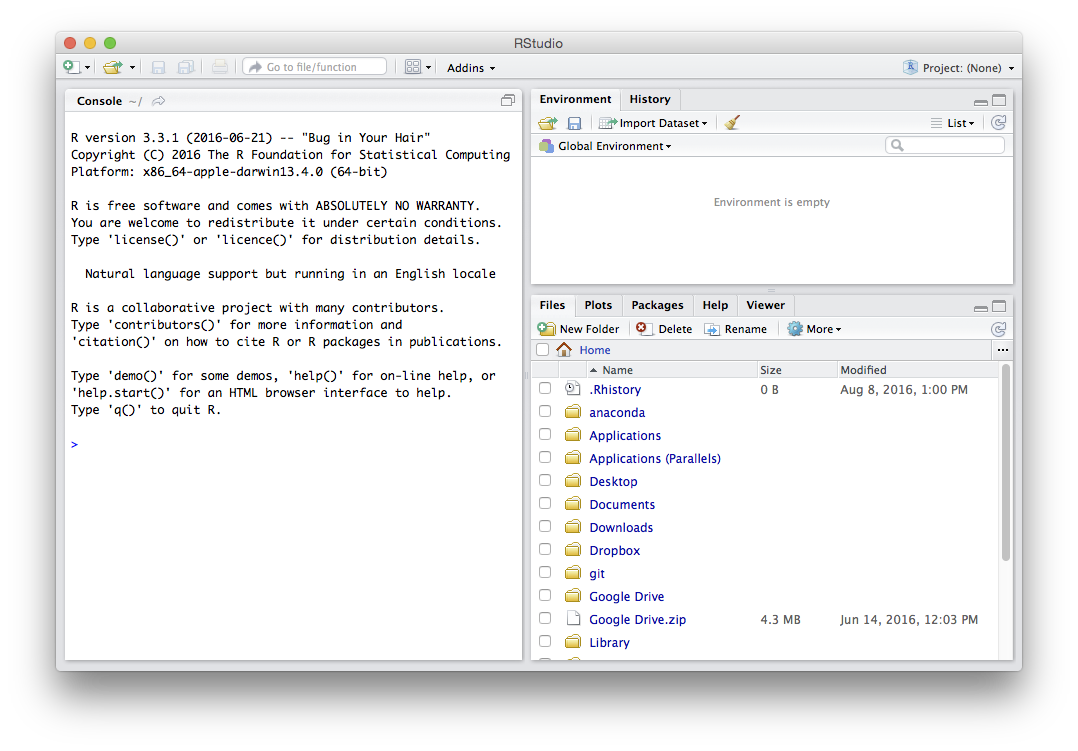
\includegraphics{R/Rinstall/images/rstudio_successful_install.png}
\caption{}
\end{figure}

\textbf{If you are having any difficulties with the installations or
your RStudio screen does not look like this one, please stop by the
training room 20 minutes prior to the start of the workshop.}

\section{\texorpdfstring{Installing the
\texttt{tidyverse}}{Installing the tidyverse}}\label{installing-the-tidyverse}

We will use the \texttt{tidyverse} suite of packages throughout these R
workshops. Here are the steps for installation:

\begin{enumerate}
\def\labelenumi{\arabic{enumi}.}
\item
  \textbf{Launch an R session within RStudio}

  On Windows, click the start button and search for RStudio then click
  on it. On Mac, RStudio will be in your applications folder --- double
  click on it.
\item
  \textbf{Install \texttt{tidyverse}}

  In the left-hand side window (called the \texttt{console}), at the
  command prompt (\texttt{\textgreater{}}) type the following and press
  enter:

  \texttt{install.packages("tidyverse")}

  \begin{itemize}
  \tightlist
  \item
    If a choice appears that says something like:
  \end{itemize}

  \texttt{Do\ you\ want\ to\ install\ from\ sources\ the\ package\ which\ needs\ compilation?}

  type \texttt{No} in the console.

  \begin{itemize}
  \tightlist
  \item
    If you are running Windows OS, you may see a message that says:
  \end{itemize}

  \texttt{WARNING:\ Rtools\ is\ required\ to\ build\ R\ packages,\ but\ is\ not\ currently\ installed.}

  You can safely ignore this warning.

  A number of messages will scroll by, and there will be a long minute
  or two pause where nothing appears to happen (but the installation is
  actually occurring). At last, the output parade should end with a
  message like:

  \texttt{The\ downloaded\ source/binary\ packages\ are\ in....}
\item
  \textbf{Check that installation was successful}

  We can check that \texttt{tidyverse} has installed correctly by
  connecting it to our current R session. Type the following in the
  console at the command prompt (\texttt{\textgreater{}}) and press
  enter:

  \texttt{library(tidyverse)}

  \textbf{Success? If so, you should see the following message in the
  console (note that the version numbers reported may be newer):}

  \begin{figure}
  \centering
  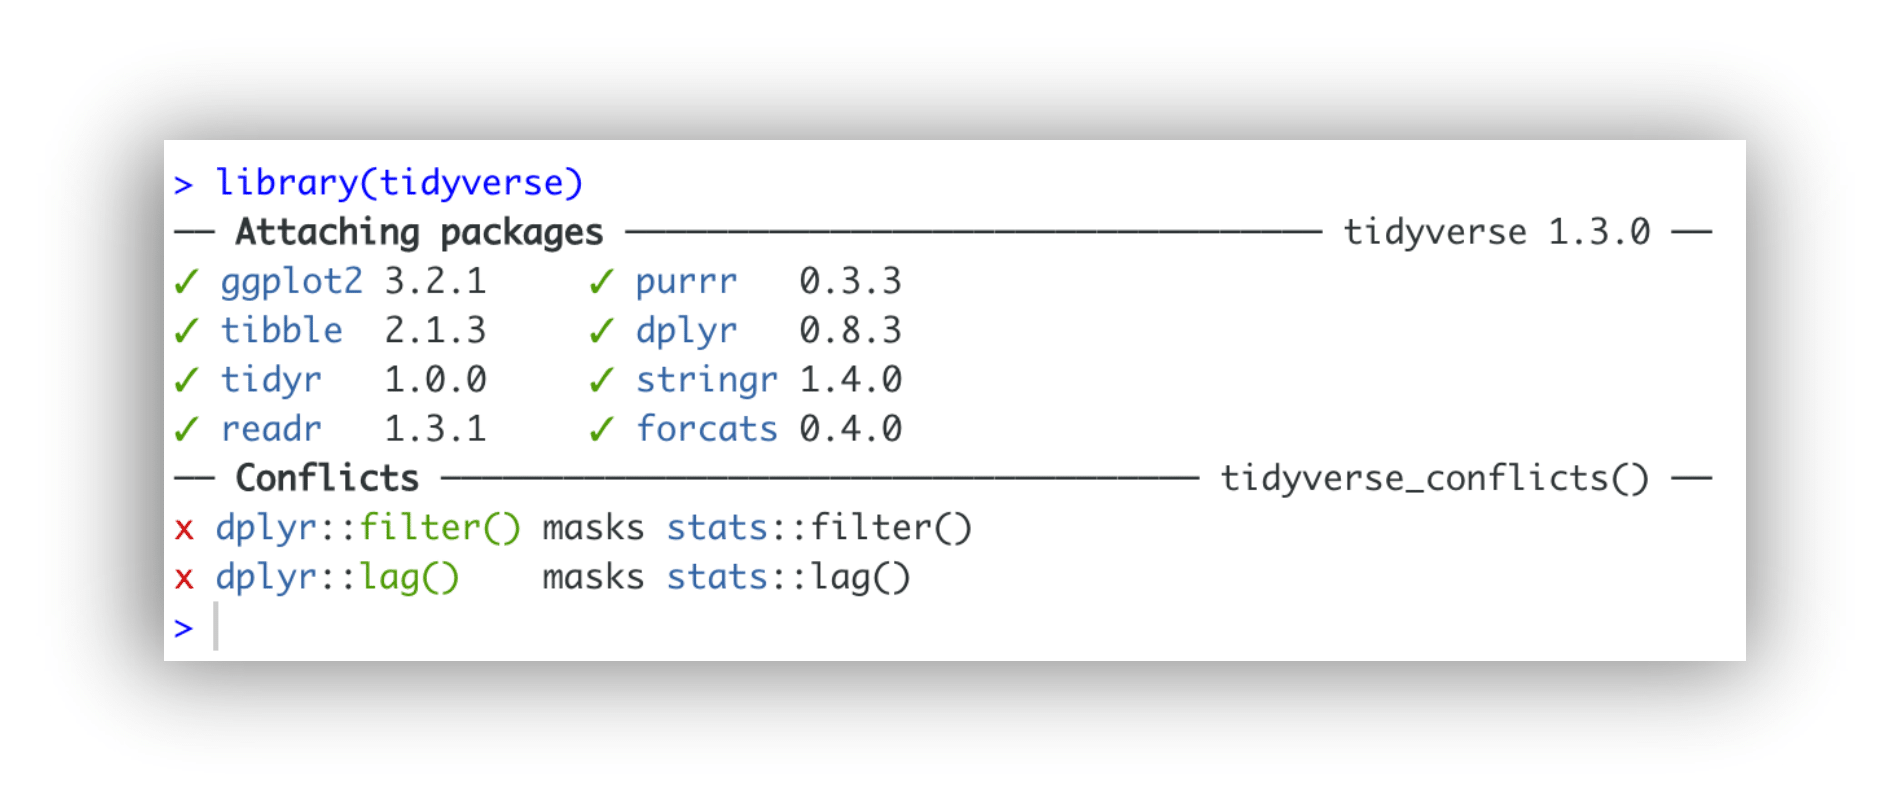
\includegraphics{R/Rinstall/images/tidyverse_install.png}
  \caption{}
  \end{figure}

  \textbf{If you do not see this message and encounter an error --- try
  troubleshooting this in the next section.}
\end{enumerate}

\subsection{\texorpdfstring{Troubleshooting \texttt{tidyverse}
installation}{Troubleshooting tidyverse installation}}\label{troubleshooting-tidyverse-installation}

Sometimes, you may run into problems installing the \texttt{tidyverse}
suite of packages. Here are some commonly encountered errors and
suggestions for how to fix them:

\begin{enumerate}
\def\labelenumi{\arabic{enumi}.}
\tightlist
\item
  \textbf{\texttt{tidyverse} is not available for R version\ldots{}}

  \begin{itemize}
  \tightlist
  \item
    Solution: make sure you have the latest versions of both R (3.6.2)
    and RStudio (1.2.5033).
  \end{itemize}
\item
  \textbf{there is no package \texttt{rlang}\ldots{}}

  \begin{itemize}
  \tightlist
  \item
    Solution: run this command in the console at the command prompt
    (\texttt{\textgreater{}}):
  \item
    \texttt{install.packages("dplyr")}
  \item
    If a choice appears that says something like
    \texttt{Do\ you\ want\ to\ install\ from\ sources\ the\ package\ which\ needs\ compilation?},
    type \texttt{No} in the console.
  \end{itemize}
\item
  \textbf{there is no package \texttt{broom}\ldots{}}

  \begin{itemize}
  \tightlist
  \item
    Solution: run these commands in the console at the command prompt
    (\texttt{\textgreater{}}), \textbf{in this order}:
  \item
    \texttt{install.packages("backports")}
  \item
    \texttt{install.packages("zeallot")}
  \item
    \texttt{install.packages("broom")}
  \item
    \texttt{install.packages("tidyverse")}
  \item
    If a choice appears at any point that says something like
    \texttt{Do\ you\ want\ to\ install\ from\ sources\ the\ package\ which\ needs\ compilation?},
    type \texttt{No} in the console.
  \end{itemize}
\item
  \textbf{rlang and/or broom still do not work}

  \begin{itemize}
  \tightlist
  \item
    Solution: load individual packages that we need from the
    \texttt{tidyverse} suite, by running the following commands in the
    console at the command prompt (\texttt{\textgreater{}}):
  \item
    \texttt{library("dplyr")} \# for the pipe function
    \%\textgreater{}\% and other SQL commands
  \item
    \texttt{library("ggplot2")} \# modern data visualization
  \item
    \texttt{library("readr")} \# to load CSV data files
  \item
    \texttt{library("tidyr")} \# to reshape data frames with functions
    like gather or spread
  \end{itemize}
\end{enumerate}

\textbf{If you have still not successfully installed \texttt{tidyverse}
(or at least \texttt{dplyr}, \texttt{ggplot2}, \texttt{readr}, and
\texttt{tidyr}) after troubleshooting, please stop by the training room
20 minutes before the start of your workshop so we can help you. Without
these packages, you will not be able to follow along with the workshop
materials.}

\section{\texorpdfstring{Installing \texttt{rmarkdown}
(optional)}{Installing rmarkdown (optional)}}\label{installing-rmarkdown-optional}

We can also install the \texttt{rmarkdown} package, which will allow us
to combine our text and code into a formatted document at the end of the
workshops. Installing this package is optional and will not affect your
ability to follow along with the workshop.

\begin{enumerate}
\def\labelenumi{\arabic{enumi}.}
\item
  \textbf{Install \texttt{rmarkdown}}

  At the command prompt in the console (\texttt{\textgreater{}}), please
  run the following command and press enter:

  \texttt{install.packages("rmarkdown")}

  then wait for the stream of messages to end with:

  \texttt{The\ downloaded\ source/binary\ packages\ are\ in....}
\item
  \textbf{Check that installation was successful}

  We can check that \texttt{rmarkdown} has installed correctly by
  connecting it to our R session. Type the following in the console at
  the command prompt (\texttt{\textgreater{}}) and press enter:

  \texttt{library(rmarkdown)}

  \textbf{Success? If so, in the console you should see just a command
  prompt (\texttt{\textgreater{}}) with no messages to the right of it.}

  \textbf{If you see error or warning messages after the command prompt,
  the installation was not successful.}
\end{enumerate}

If all the above steps have been completed successfully, you should now
be ready to start your workshop. \textbf{If you ran into any problems,
please stop by the training room 20 minutes before the start of your
workshop.}

\section{Resources}\label{resources-1}

\begin{itemize}
\tightlist
\item
  IQSS

  \begin{itemize}
  \tightlist
  \item
    Workshops: \url{https://dss.iq.harvard.edu/workshop-materials}
  \item
    Data Science Services: \url{https://dss.iq.harvard.edu/}
  \item
    Research Computing Environment:
    \url{https://iqss.github.io/dss-rce/}
  \end{itemize}
\item
  HBS

  \begin{itemize}
  \tightlist
  \item
    Research Computing Services workshops:
    \url{https://training.rcs.hbs.org/workshops}
  \item
    Other HBS RCS resources:
    \url{https://training.rcs.hbs.org/workshop-materials}
  \item
    RCS consulting email: \url{mailto:research@hbs.edu}
  \end{itemize}
\end{itemize}

\chapter{R Introduction}\label{r-introduction}

\textbf{Topics}

\begin{itemize}
\tightlist
\item
  Functions
\item
  Objects
\item
  Assignment
\item
  Finding help
\item
  Importing packages
\item
  Basic data manipulation
\item
  Operations within groups of data
\item
  Saving data
\end{itemize}

\section{Setup}\label{setup}

\subsection{Class Structure}\label{class-structure}

\begin{itemize}
\tightlist
\item
  Informal --- Ask questions at any time. Really!
\item
  Collaboration is encouraged - please spend a minute introducing
  yourself to your neighbors!
\end{itemize}

\subsection{Prerequisites}\label{prerequisites}

This is an introductory R course:

\begin{itemize}
\tightlist
\item
  Assumes no prior knowledge of \textbf{how to use} R
\item
  We do assume you know \textbf{why} you want to learn R. If you don't,
  and want a comparison of R to other statistical software, see our
  \href{./DataScienceTools.html}{Data Science Tools} workshop
\item
  Relatively slow-paced
\end{itemize}

\subsection{Goals}\label{goals}

We will learn about the R language by analyzing a dataset of baby names.
In particular, our goals are to learn about:

\begin{enumerate}
\def\labelenumi{\arabic{enumi}.}
\tightlist
\item
  What R is and how it works
\item
  How we can interact with R
\item
  Foundations of the language (functions, objects, assignment)
\item
  The \texttt{tidyverse} package ecosystem for data science
\item
  Basic data manipulation useful for cleaning datasets
\item
  Working with grouped data
\item
  Aggregating data to create summaries
\item
  Saving objects, data, and scripts
\end{enumerate}

This workshop will not cover how to iterate over collections of data,
create your own functions, produce publication quality graphics, or fit
models to data. These topics are covered in our
\href{./RDataWrangling.html}{R Data Wrangling},
\href{./Rgraphics.html}{R Graphics}, and \href{./Rmodels.html}{R
Regression Models} workshops.

\section{R basics}\label{r-basics}

\textbf{GOAL: To learn about the foundations of the R language.} In
particular:

\begin{enumerate}
\def\labelenumi{\arabic{enumi}.}
\tightlist
\item
  What R is and how it works
\item
  R interfaces
\item
  Functions
\item
  Objects
\item
  Assignment
\item
  Getting help
\item
  \texttt{tidyverse} package ecosystem for data science
\end{enumerate}

\subsection{What is R?}\label{what-is-r}

\begin{itemize}
\tightlist
\item
  R is a free language and environment for statistical computing and
  graphics
\item
  R is an interpreted language, not a compiled one, meaning that all
  commands typed on the keyboard are directly executed without requiring
  to build a complete program (this is like Python and unlike C,
  Fortran, Pascal, etc.)
\item
  R has existed for over 25 years
\item
  R is modular --- most functionality is from add-on packages. So the
  language can be thought of as a \emph{platform} for creating and
  running a large number of useful packages.
\end{itemize}

\subsection{Why use R?}\label{why-use-r}

\begin{itemize}
\tightlist
\item
  The most popular software for data analysis
\item
  Extremely flexible: can be used to manipulate, analyze, and visualize
  any kind of data
\item
  Cutting edge statistical tools
\item
  Publication quality graphics
\item
  15,000+ add on packages covering all aspects of statistics and machine
  learning
\item
  Active community of users
\end{itemize}

\subsection{How does R work?}\label{how-does-r-work}

While graphical-based statistical software (e.g., SPSS, GraphPad)
immediately display the results of an analysis, \textbf{R stores results
in an \texttt{object} (a data structure)}, so that an analysis can be
done with no result displayed. Such a feature is very useful, since a
user can extract only that part of the results that is of interest and
can pass results into further analyses.

For example, if you run a series of 20 regressions and want to compare
the different regression coefficients, R can display only the estimated
coefficients: thus the results may take a single line, whereas
graphical-based software could open 20 results windows. In addition,
these regression coefficients can be passed directly into further
analyses --- such as generating predictions.

\begin{figure}
\centering
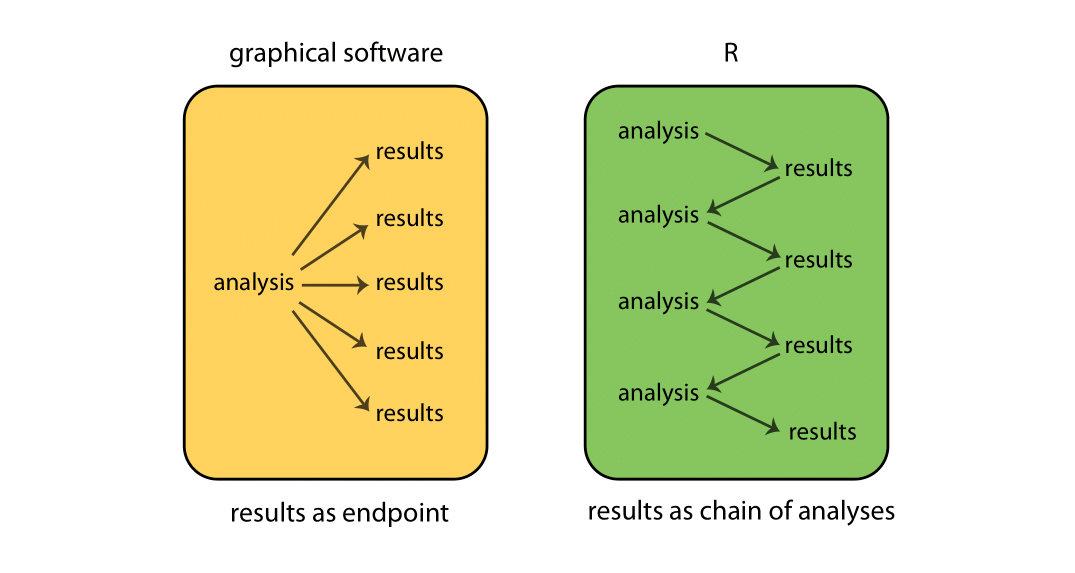
\includegraphics{R/Rintro/images/R_chain.png}
\caption{}
\end{figure}

When R is running, variables, data, functions, results, etc., are
\textbf{stored in memory} on the computer in the form of
\texttt{objects} that have a name. The user can \textbf{perform actions}
on these objects with \texttt{operators} (arithmetic, logical,
comparison, etc.) and \texttt{functions} (which are themselves objects).
Here's a schematic of how this all fits together:

\begin{figure}
\centering
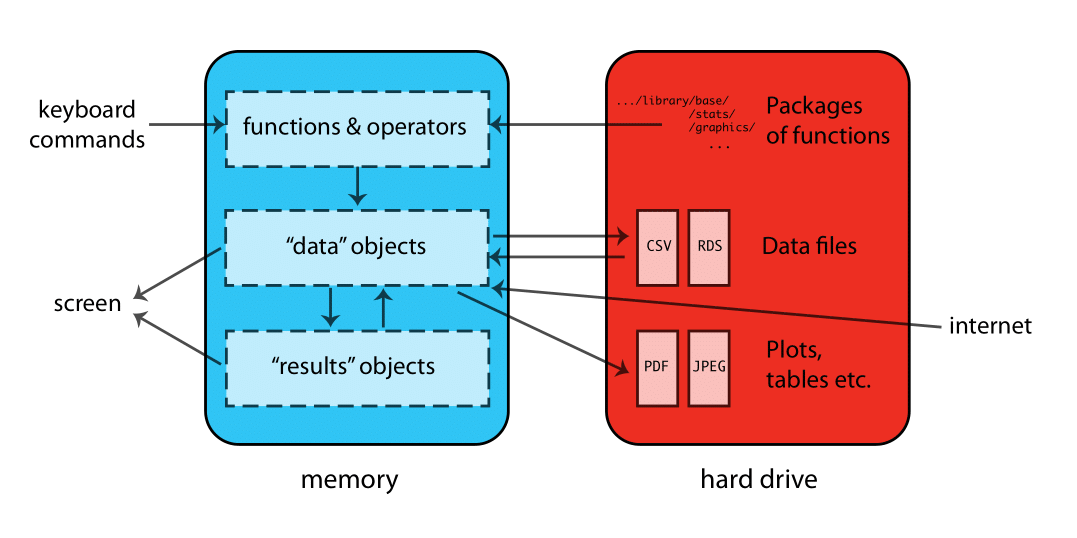
\includegraphics{R/Rintro/images/R_works.png}
\caption{}
\end{figure}

\subsection{Interfaces}\label{interfaces}

\subsubsection{Text editors, IDEs, \&
Notebooks}\label{text-editors-ides-notebooks}

There are different ways of interacting with R. The two main ways are
through:

\begin{enumerate}
\def\labelenumi{\arabic{enumi}.}
\item
  \textbf{text editors} or \textbf{Integrated Development Environments
  (IDEs):} Text editors and IDEs are not really separate categories; as
  you add features to a text editor it becomes more like an IDE. Some
  editors/IDEs are language-specific while others are general purpose
  --- typically providing language support via plugins. For these
  workshops we will use \href{https://rstudio.com/}{RStudio}; it is a
  good R-specific IDE with many useful features. Here are a few popular
  editors/IDEs that can be used with R:

  \begin{longtable}[]{@{}llll@{}}
  \toprule
  Editor / IDE & Features & Ease of use & Language
  support\tabularnewline
  \midrule
  \endhead
  RStudio & Excellent & Easy & R only\tabularnewline
  Jupyter Lab & Good & Easy & Excellent\tabularnewline
  VS code & Excellent & Easy & Very good\tabularnewline
  Atom & Good & Moderate & Good\tabularnewline
  Vim & Excellent & Hard & Good\tabularnewline
  Emacs & Excellent & Hard & Excellent\tabularnewline
  \bottomrule
  \end{longtable}
\item
  \textbf{Notebooks:} Web-based applications that allow you to create
  and share documents that contain live code, equations, visualizations,
  and narrative text. A popular notebook is the open source
  \href{https://jupyter.org/}{Jupyter Notebook} that has support for 40+
  languages.
\end{enumerate}

\subsubsection{Source code \& literate
programming}\label{source-code-literate-programming}

There are also several different \textbf{formats} available for writing
code in R. These basically boil down to a choice between:

\begin{enumerate}
\def\labelenumi{\arabic{enumi}.}
\item
  \textbf{Source code:} the practice of writing code, and possibly
  comments, in a plain text document. In R this is done by writing code
  in a text file with a \texttt{.R} or \texttt{.r} extension. Writing
  source code has the great advantage of being simple. Souce code is the
  format of choice if you intend to run your code as a complete script -
  for example, from the command line.
\item
  \textbf{Literate programming:} the practice of embedding computer code
  in a natural language document. In R this is often done using
  \href{https://rmarkdown.rstudio.com/}{\textbf{Rmarkdown}}, which
  involves embeddeding R code in a document that is authored using
  \emph{Markdown} and which has a \texttt{.Rmd} extension.
  \emph{Markdown} is easy to write and designed to be human-readable.
  Markdown is the format of choice if you intend to run your code
  interactively, by running small pieces of code and looking at each
  output. Many researchers use Markdown to write their journal papers,
  dissertations, and statistics/math class notes, since it is easy to
  convert into other formats later, such as HTML (for a webpage), MS
  Word, or PDF (via LaTeX).
\end{enumerate}

Here are some resources for learning more about Rmarkdown and RStudio:

\begin{itemize}
\tightlist
\item
  \url{https://rmarkdown.rstudio.com/authoring_quick_tour.html}
\item
  \url{https://cran.r-project.org/web/packages/rmarkdown/vignettes/rmarkdown.html}
\item
  \url{https://rstudio.com/wp-content/uploads/2019/01/Cheatsheets_2019.pdf}
\end{itemize}

\subsection{Launch a session}\label{launch-a-session}

Start RStudio and create a new project:

\begin{itemize}
\tightlist
\item
  On Windows click the start button and search for RStudio. On Mac
  RStudio will be in your applications folder.
\item
  In Rstudio go to \texttt{File\ -\textgreater{}\ New\ Project}.
\item
  Choose \texttt{Existing\ Directory} and browse to the workshop
  materials directory on your desktop.
\item
  Choose \texttt{File\ -\textgreater{}\ Open\ File} and select the file
  with the word ``BLANK'' in the name.
\end{itemize}

\subsection{Exercise 0}\label{exercise-0}

The purpose of this exercise is to give you an opportunity to explore
the interface provided by RStudio. You may not know how to do these
things; that's fine! This is an opportunity to figure it out.

Also keep in mind that we are living in a golden age of tab completion.
If you don't know the name of an R function, try guessing the first two
or three letters and pressing TAB. If you guessed correctly the function
you are looking for should appear in a pop up!

\begin{enumerate}
\def\labelenumi{\arabic{enumi}.}
\item
  Try to get R to add 2 plus 2.

\begin{Shaded}
\begin{Highlighting}[]
\NormalTok{##}
\end{Highlighting}
\end{Shaded}
\item
  Try to calculate the square root of 10.

\begin{Shaded}
\begin{Highlighting}[]
\NormalTok{##}
\end{Highlighting}
\end{Shaded}
\item
  R includes extensive documentation, including a manual named ``An
  introduction to R''. Use the RStudio help pane. to locate this manual.
\end{enumerate}

\subsection{Syntax rules}\label{syntax-rules}

\begin{itemize}
\tightlist
\item
  R is case sensitive
\item
  R ignores white space
\item
  Variable names should start with a letter (A-Z and a-z) and can
  include letters, digits (0-9), dots (.), and underscores (\_)
\item
  Comments can be inserted using a hash \texttt{\#} symbol
\item
  Functions must be written with parentheses, even if there is nothing
  within them; for example: \texttt{ls()}
\end{itemize}

\subsection{Function calls}\label{function-calls}

\textbf{Functions perform actions} --- they take some input, called
\texttt{arguments} and return some output (i.e., a result). Here's a
schematic of how a function works:

\begin{figure}
\centering
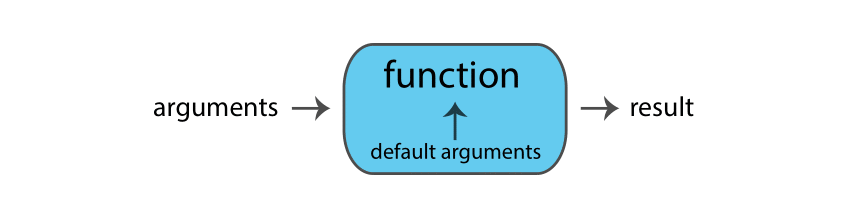
\includegraphics{R/Rintro/images/function.png}
\caption{}
\end{figure}

The general form for calling R functions is

\begin{Shaded}
\begin{Highlighting}[]
\NormalTok{## FunctionName(arg.1 = value.1, arg.2 = value.2, ..., arg.n = value.n)}
\end{Highlighting}
\end{Shaded}

The arguments in a function can be objects (data, formulae, expressions,
etc.), some of which could be defined by default in the function; these
default values may be modified by the user by specifying options.

Arguments can be \textbf{matched by name}; unnamed arguments will be
\textbf{matched by position}.

\begin{Shaded}
\begin{Highlighting}[]
\NormalTok{values <-}\StringTok{ }\KeywordTok{c}\NormalTok{(}\FloatTok{1.45}\NormalTok{, }\FloatTok{2.34}\NormalTok{, }\FloatTok{5.68}\NormalTok{)}
\KeywordTok{round}\NormalTok{(}\DataTypeTok{x =}\NormalTok{ values, }\DataTypeTok{digits =} \DecValTok{1}\NormalTok{) }\CommentTok{# match by name}
\end{Highlighting}
\end{Shaded}

\begin{verbatim}
## [1] 1.4 2.3 5.7
\end{verbatim}

\begin{Shaded}
\begin{Highlighting}[]
\KeywordTok{round}\NormalTok{(values, }\DecValTok{1}\NormalTok{) }\CommentTok{# match by position}
\end{Highlighting}
\end{Shaded}

\begin{verbatim}
## [1] 1.4 2.3 5.7
\end{verbatim}

\begin{Shaded}
\begin{Highlighting}[]
\KeywordTok{round}\NormalTok{(}\DecValTok{1}\NormalTok{, values) }\CommentTok{# be careful when matching by position!}
\end{Highlighting}
\end{Shaded}

\begin{verbatim}
## [1] 1 1 1
\end{verbatim}

\begin{Shaded}
\begin{Highlighting}[]
\KeywordTok{round}\NormalTok{(}\DataTypeTok{digits =} \DecValTok{1}\NormalTok{, }\DataTypeTok{x =}\NormalTok{ values) }\CommentTok{# matching by name is safer!}
\end{Highlighting}
\end{Shaded}

\begin{verbatim}
## [1] 1.4 2.3 5.7
\end{verbatim}

\subsection{Assignment}\label{assignment}

Values can be assigned names and used in subsequent operations

\begin{itemize}
\tightlist
\item
  The \textbf{gets} \texttt{\textless{}-} operator (less than followed
  by a dash) is used to save values
\item
  The name on the left \textbf{gets} the value on the right.
\end{itemize}

\begin{Shaded}
\begin{Highlighting}[]
\KeywordTok{sqrt}\NormalTok{(}\DecValTok{10}\NormalTok{) ## calculate square root of 10; result is not stored anywhere}
\end{Highlighting}
\end{Shaded}

\begin{verbatim}
## [1] 3.16228
\end{verbatim}

\begin{Shaded}
\begin{Highlighting}[]
\NormalTok{x <-}\StringTok{ }\KeywordTok{sqrt}\NormalTok{(}\DecValTok{10}\NormalTok{) }\CommentTok{# assign result to a variable named x}
\end{Highlighting}
\end{Shaded}

Names should start with a letter, and contain only letters, numbers,
underscores, and periods.

\subsection{Asking for help}\label{asking-for-help}

\begin{enumerate}
\def\labelenumi{\arabic{enumi}.}
\item
  You can ask R for help using the \texttt{help} function, or the
  \texttt{?} shortcut.

\begin{Shaded}
\begin{Highlighting}[]
\KeywordTok{help}\NormalTok{(help)}
\NormalTok{?help}
\NormalTok{?sqrt}
\end{Highlighting}
\end{Shaded}

  The \texttt{help} function can be used to look up the documentation
  for a function, or to look up the documentation to a package. We can
  learn how to use the \texttt{stats} package by reading its
  documentation like this:

\begin{Shaded}
\begin{Highlighting}[]
\KeywordTok{help}\NormalTok{(}\DataTypeTok{package =} \StringTok{"stats"}\NormalTok{)}
\end{Highlighting}
\end{Shaded}
\item
  If you know the name of the package you want to use, then Googling ``R
  \emph{package-name}'' will often get you to the documentation.
  Packages are hosted on several different repositories, including:

  \begin{itemize}
  \tightlist
  \item
    CRAN:
    \url{https://cran.r-project.org/web/packages/available_packages_by_name.html}
  \item
    Bioconductor:
    \url{https://www.bioconductor.org/packages/release/bioc/}
  \item
    Github: \url{http://rpkg.gepuro.net/}
  \item
    R-Forge: \url{https://r-forge.r-project.org/R/?group_id=1326}
  \end{itemize}
\item
  If you know the type of analysis you want to perform, you can Google
  ``CRAN Task Views'', where there are curated lists of packages
  \url{https://cran.r-project.org/web/views/}. If you want to know which
  packages are popular, you can look at \url{https://r-pkg.org}.
\end{enumerate}

\subsection{Reading data}\label{reading-data}

R has data reading functionality built-in -- see e.g.,
\texttt{help(read.table)}. However, faster and more robust tools are
available, and so to make things easier on ourselves we will use a
\emph{contributed package} instead. This requires that we learn a little
bit about packages in R.

\subsection{Installing \& using
packages}\label{installing-using-packages}

R is a modular environment that is extended by the use of
\textbf{packages}. Packages are collections of functions or commands
that are designed to perform specific tasks (e.g., fit a type of
regression model). A large number of contributed packages are available
(\textgreater{} 15,000).

Using an R package is a \textbf{two step process}:

\begin{enumerate}
\def\labelenumi{\arabic{enumi}.}
\item
  Install the package onto your computer using the
  \texttt{install.packages()} function. This only needs to be done the
  \textbf{first time} you use the package.
\item
  Load the package into your R session's search path using the
  \texttt{library()} function. This needs to be done \textbf{each time}
  you use the package.
\end{enumerate}

\subsection{\texorpdfstring{The
\texttt{tidyverse}}{The tidyverse}}\label{the-tidyverse}

While R's built-in packages are powerful, in recent years there has been
a big surge in well-designed \emph{contributed packages} for R. In
particular, a collection of R packages called
\href{https://www.tidyverse.org/}{\texttt{tidyverse}} have been designed
specifically for data science. All packages included in
\texttt{tidyverse} share an underlying design philosophy, grammar, and
data structures. This philosopy is rooted in the idea of ``tidy data'':

\begin{figure}
\centering
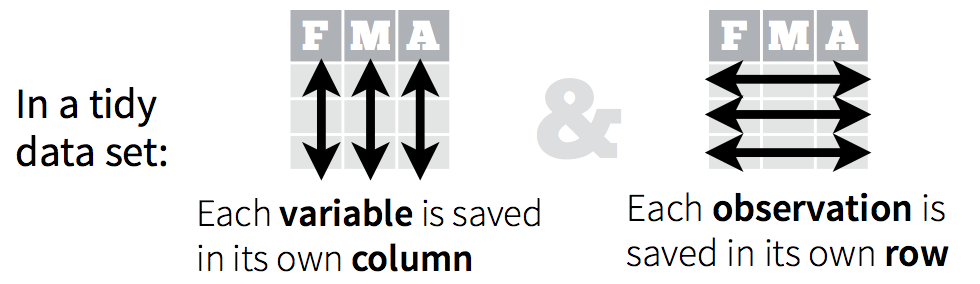
\includegraphics{R/Rintro/images/tidy_data.png}
\caption{}
\end{figure}

A typical workflow for using \texttt{tidyverse} packages looks like
this:

\begin{figure}
\centering
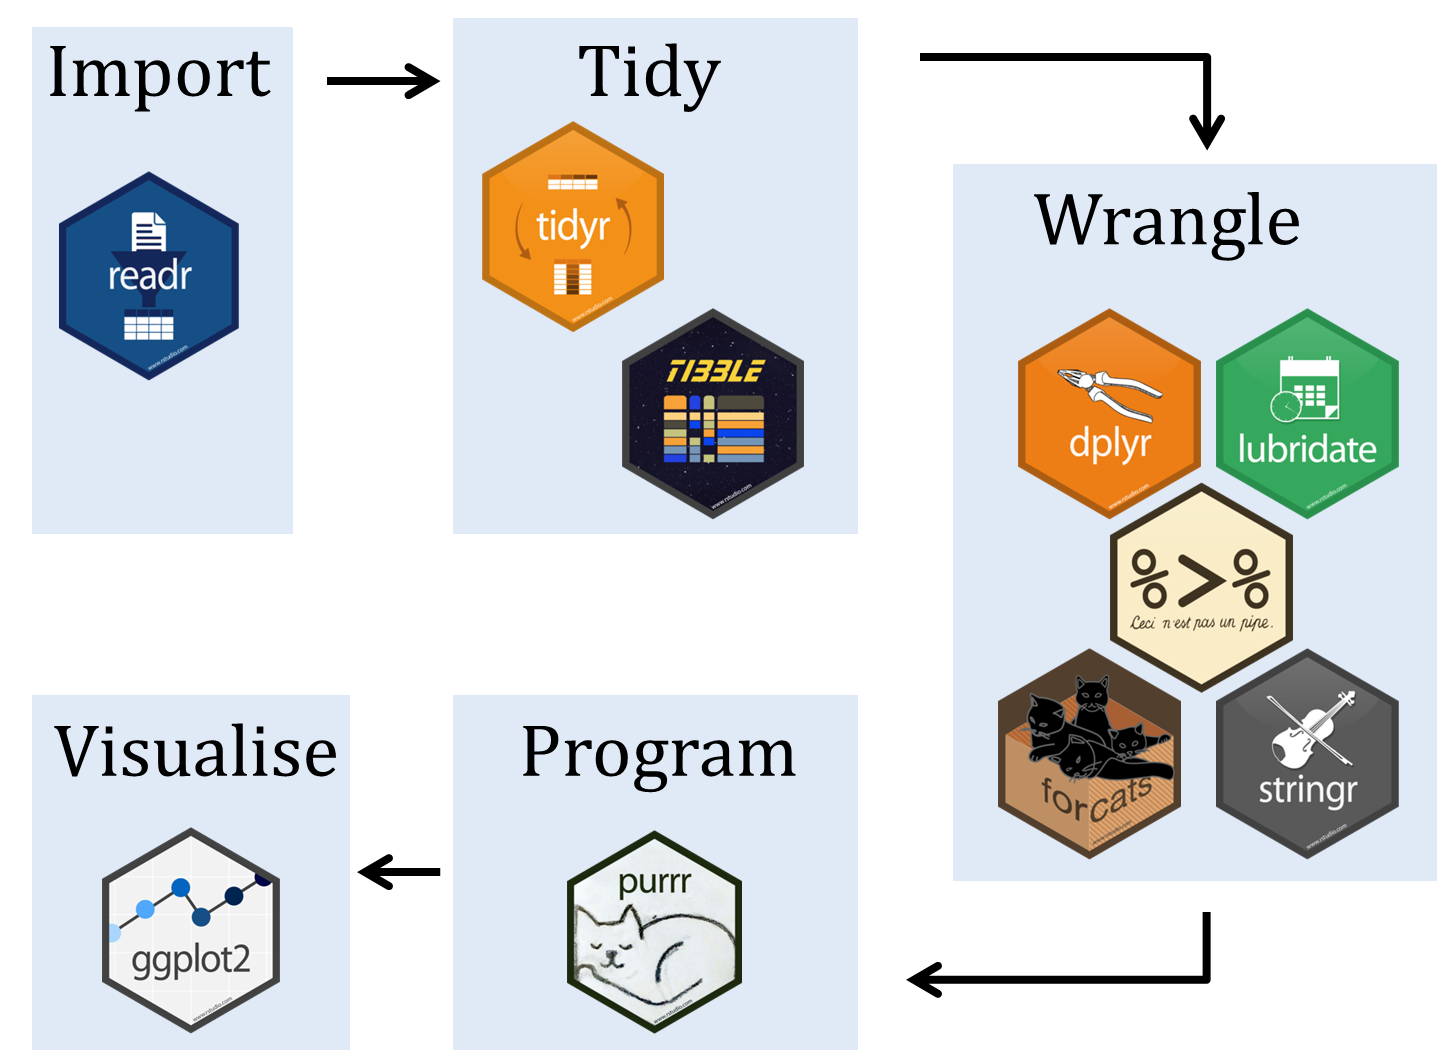
\includegraphics{R/Rintro/images/tidy_workflow.png}
\caption{}
\end{figure}

You should have already installed the \texttt{tidyverse} and
\texttt{rmarkdown} packages onto your computer before the workshop ---
see \href{./Rinstall.html}{R Installation}. Now let's load these
packages into the search path of our R session.

\begin{Shaded}
\begin{Highlighting}[]
\KeywordTok{library}\NormalTok{(tidyverse)}
\KeywordTok{library}\NormalTok{(rmarkdown)}
\end{Highlighting}
\end{Shaded}

\subsection{Readers for common file
types}\label{readers-for-common-file-types}

To read data from a file, you have to know what kind of file it is. The
table below lists functions from the \texttt{readr} package, which is
part of \texttt{tidyverse}, that can import data from common plain-text
formats.

\begin{longtable}[]{@{}ll@{}}
\toprule
Data Type & Function\tabularnewline
\midrule
\endhead
comma separated & \texttt{read\_csv()}\tabularnewline
tab separated & \texttt{read\_delim()}\tabularnewline
other delimited formats & \texttt{read\_table()}\tabularnewline
fixed width & \texttt{read\_fwf()}\tabularnewline
\bottomrule
\end{longtable}

\textbf{Note} You may be confused by the existence of similar functions,
e.g., \texttt{read.csv} and \texttt{read.delim}. These are legacy
functions that tend to be slower and less robust than the \texttt{readr}
functions. One way to tell them apart is that the faster more robust
versions use underscores in their names (e.g., \texttt{read\_csv}) while
the older functions use dots (e.g., \texttt{read.csv}). My advice is to
use the more robust newer versions, i.e., the ones with underscores.

\subsection{Baby names data}\label{baby-names-data}

As an example project we will analyze the popularity of baby names in
the US from 1960 through 2017. The data were retrieved from
\url{https://catalog.data.gov/dataset/baby-names-from-social-security-card-applications-national-level-data}.

Here are the questions we will use R to answer:

\begin{enumerate}
\def\labelenumi{\arabic{enumi}.}
\tightlist
\item
  In which year did your name (or another name) occur most frequently by
  \textbf{count}?
\item
  Which names have the highest popularity by \textbf{proportion} for
  each sex and year?
\item
  How does the percentage of babies given one of the top 10 names of the
  year change over time?
\end{enumerate}

\subsection{Exercise 1}\label{exercise-1}

\textbf{Reading the baby names data}

Make sure you have installed the \texttt{tidyverse} suite of packages
and attached them with \texttt{library(tidyverse)}.

\begin{enumerate}
\def\labelenumi{\arabic{enumi}.}
\item
  Open the \texttt{read\_csv()} help page to determine how to use it to
  read in data.

\begin{Shaded}
\begin{Highlighting}[]
\NormalTok{##}
\end{Highlighting}
\end{Shaded}
\item
  Read the baby names data using the \texttt{read\_csv()} function and
  assign the result with the name \texttt{baby\_names}.

\begin{Shaded}
\begin{Highlighting}[]
\NormalTok{##}
\end{Highlighting}
\end{Shaded}
\item
  BONUS (optional): Save the \texttt{baby\_names} data as a Stata data
  set \texttt{babynames.dta} and as an R data set
  \texttt{babynames.rds}.

\begin{Shaded}
\begin{Highlighting}[]
\NormalTok{##}
\end{Highlighting}
\end{Shaded}
\end{enumerate}

\section{Manipulating data}\label{manipulating-data}

\textbf{GOAL: To learn about basic data manipulation used to clean
datasets.} In particular:

\begin{enumerate}
\def\labelenumi{\arabic{enumi}.}
\tightlist
\item
  Filtering data by choosing rows --- using the \texttt{filter()}
  function
\item
  Selecting data by choosing columns --- using the \texttt{select()}
  function
\item
  Arranging data by reordering rows --- using the \texttt{arrange()}
  function
\item
  Using the pipe \texttt{\%\textgreater{}\%} operator to simplify
  sequential operations
\end{enumerate}

In this section we will pull out specific names from the baby names data
and examine changes in their popularity over time.

The \texttt{baby\_names} object we created in the last exercise is a
\texttt{data.frame}. There are many other data structures in R, but for
now we'll focus on working with \texttt{data.frames}. Think of a
\texttt{data.frame} as a spreadsheet. If you want to know more about R
data structures, you can see a summary in our
\href{./RDataWrangling.html\#data-types-and-structures}{R Data
Wrangling} workshop.

R has decent data manipulation tools built-in -- see e.g.,
\texttt{help(Extract)}. But, \texttt{tidyverse} packages often provide
more intuitive syntax for accomplishing the same task. In particular, we
will use the \texttt{dplyr} package from \texttt{tidyverse} to filter,
select, and arrange data, as well as create new variables.

\begin{figure}
\centering
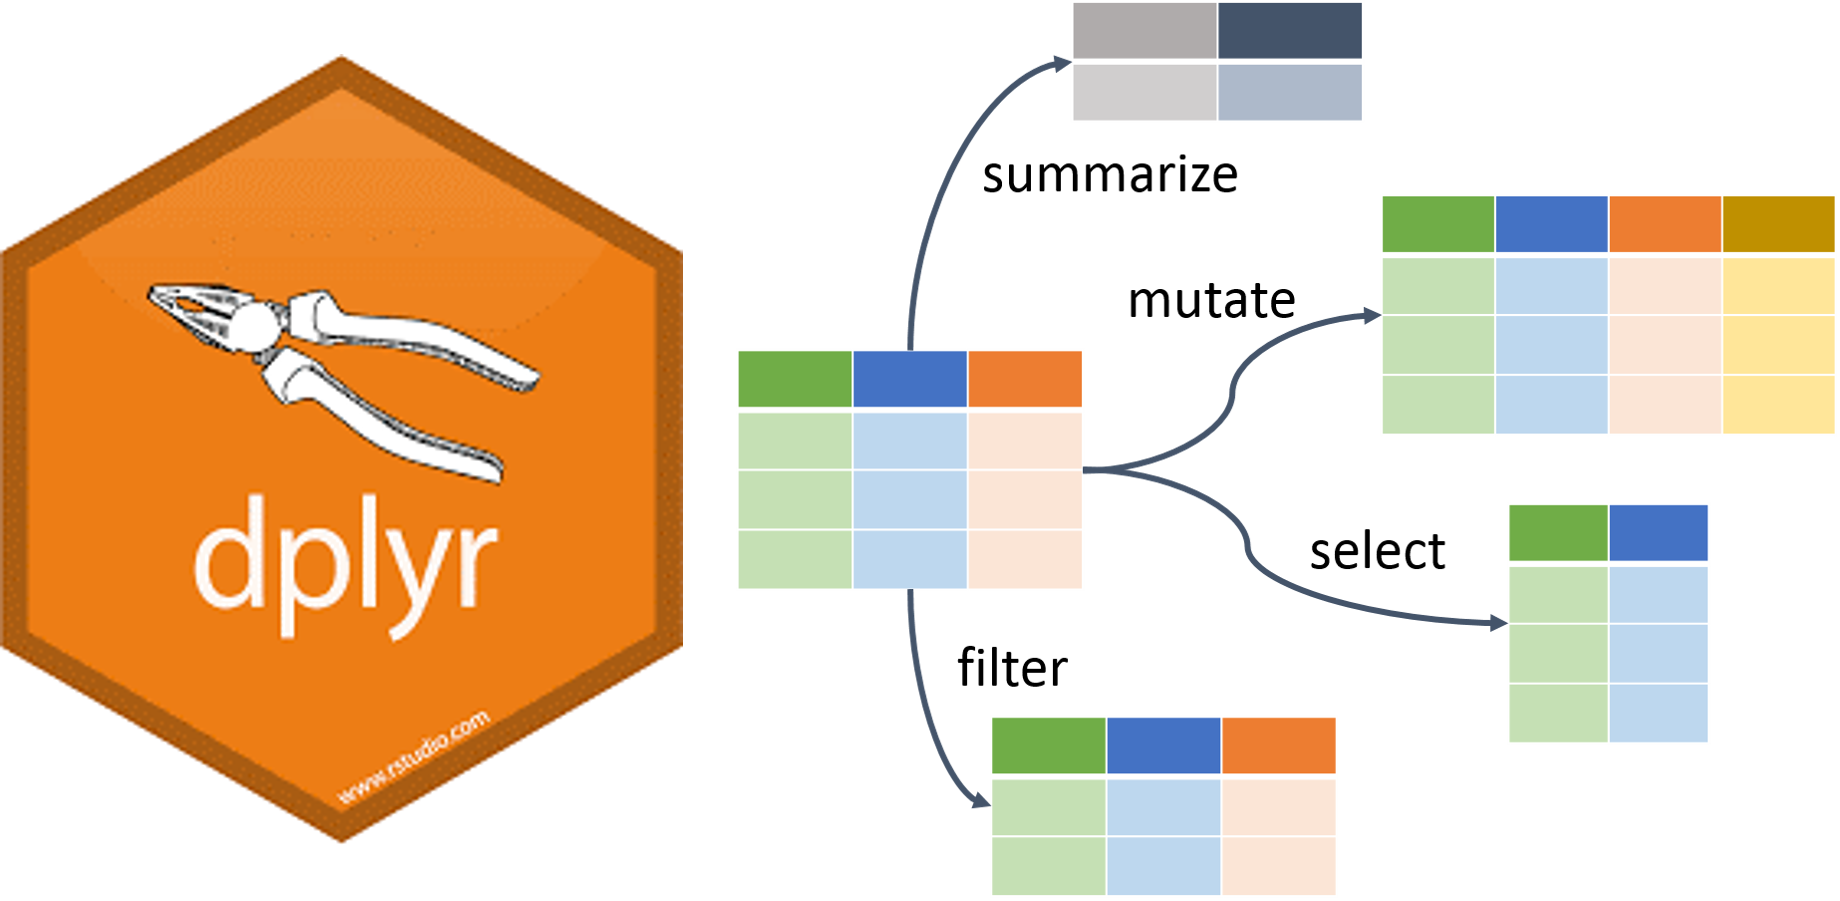
\includegraphics{R/Rintro/images/dplyr.png}
\caption{}
\end{figure}

\subsection{Filter, select, \& arrange}\label{filter-select-arrange}

One way to find the year in which your name was the most popular is to
filter out just the rows corresponding to your name, and then arrange
(sort) by Count.

To demonstrate these techniques we'll try to determine whether ``Alex''"
or ``Mark'' was more popular in 1992. We start by filtering the data so
that we keep only rows where Year is equal to \texttt{1992} and Name is
either ``Alex'' or ``Mark''.

\begin{Shaded}
\begin{Highlighting}[]
\NormalTok{## Read in the baby names data if you haven't already}
\NormalTok{baby_names <-}\StringTok{ }\KeywordTok{read_csv}\NormalTok{(}\StringTok{"babyNames.csv"}\NormalTok{)}
\end{Highlighting}
\end{Shaded}

\begin{Shaded}
\begin{Highlighting}[]
\NormalTok{baby_names_alexmark <-}\StringTok{ }\KeywordTok{filter}\NormalTok{(baby_names, }
\NormalTok{             Year }\OperatorTok{==}\StringTok{ }\DecValTok{1992} \OperatorTok{&}\StringTok{ }\NormalTok{(Name }\OperatorTok{==}\StringTok{ "Alex"} \OperatorTok{|}\StringTok{ }\NormalTok{Name }\OperatorTok{==}\StringTok{ "Mark"}\NormalTok{))}

\KeywordTok{print}\NormalTok{(baby_names_alexmark) }\CommentTok{# explicit printing}
\end{Highlighting}
\end{Shaded}

\begin{verbatim}
## # A tibble: 4 x 4
##   Name  Sex   Count  Year
##   <chr> <chr> <dbl> <dbl>
## 1 Alex  Girls   366  1992
## 2 Mark  Girls    20  1992
## 3 Mark  Boys   8743  1992
## 4 Alex  Boys   7348  1992
\end{verbatim}

\begin{Shaded}
\begin{Highlighting}[]
\NormalTok{baby_names_alexmark }\CommentTok{# implicit printing}
\end{Highlighting}
\end{Shaded}

\begin{verbatim}
## # A tibble: 4 x 4
##   Name  Sex   Count  Year
##   <chr> <chr> <dbl> <dbl>
## 1 Alex  Girls   366  1992
## 2 Mark  Girls    20  1992
## 3 Mark  Boys   8743  1992
## 4 Alex  Boys   7348  1992
\end{verbatim}

Notice that we can combine conditions using \texttt{\&} (AND) and
\texttt{\textbar{}} (OR).

In this case it's pretty easy to see that ``Mark'' is more popular, but
to make it even easier we can arrange the data so that the most popular
name is listed first.

\begin{Shaded}
\begin{Highlighting}[]
\KeywordTok{arrange}\NormalTok{(baby_names_alexmark, Count)}
\end{Highlighting}
\end{Shaded}

\begin{verbatim}
## # A tibble: 4 x 4
##   Name  Sex   Count  Year
##   <chr> <chr> <dbl> <dbl>
## 1 Mark  Girls    20  1992
## 2 Alex  Girls   366  1992
## 3 Alex  Boys   7348  1992
## 4 Mark  Boys   8743  1992
\end{verbatim}

\begin{Shaded}
\begin{Highlighting}[]
\KeywordTok{arrange}\NormalTok{(baby_names_alexmark, }\KeywordTok{desc}\NormalTok{(Count))}
\end{Highlighting}
\end{Shaded}

\begin{verbatim}
## # A tibble: 4 x 4
##   Name  Sex   Count  Year
##   <chr> <chr> <dbl> <dbl>
## 1 Mark  Boys   8743  1992
## 2 Alex  Boys   7348  1992
## 3 Alex  Girls   366  1992
## 4 Mark  Girls    20  1992
\end{verbatim}

We can also use the \texttt{select()} function to subset the
\texttt{data.frame} by columns. We can then assign the output to a new
object. If we would just like to glance at the first few lines we can
use the \texttt{head()} function:

\begin{Shaded}
\begin{Highlighting}[]
\NormalTok{baby_names_subset <-}\StringTok{ }\KeywordTok{select}\NormalTok{(baby_names, Name, Count)}

\KeywordTok{head}\NormalTok{(baby_names_subset)}
\end{Highlighting}
\end{Shaded}

\begin{verbatim}
## # A tibble: 6 x 2
##   Name  Count
##   <chr> <dbl>
## 1 Mary  51474
## 2 Susan 39200
## 3 Linda 37314
## 4 Karen 36376
## 5 Donna 34133
## 6 Lisa  33702
\end{verbatim}

\begin{Shaded}
\begin{Highlighting}[]
\KeywordTok{head}\NormalTok{(baby_names_subset, }\DataTypeTok{n =} \DecValTok{6}\NormalTok{) }\CommentTok{# default is n = 6}
\end{Highlighting}
\end{Shaded}

\begin{verbatim}
## # A tibble: 6 x 2
##   Name  Count
##   <chr> <dbl>
## 1 Mary  51474
## 2 Susan 39200
## 3 Linda 37314
## 4 Karen 36376
## 5 Donna 34133
## 6 Lisa  33702
\end{verbatim}

\subsection{Logical \& relational
operators}\label{logical-relational-operators}

In a previous example we used \texttt{==} to filter rows. Here's a table
of other commonly used relational operators:

\begin{longtable}[]{@{}ll@{}}
\toprule
Operator & Meaning\tabularnewline
\midrule
\endhead
\texttt{==} & equal to\tabularnewline
\texttt{!=} & not equal to\tabularnewline
\texttt{\textgreater{}} & greater than\tabularnewline
\texttt{\textgreater{}=} & greater than or equal to\tabularnewline
\texttt{\textless{}} & less than\tabularnewline
\texttt{\textless{}=} & less than or equal to\tabularnewline
\texttt{\%in\%} & contained in\tabularnewline
\bottomrule
\end{longtable}

These relational operators may be combined with logical operators, such
as \texttt{\&} (and) or \texttt{\textbar{}} (or). For example, we can
create a \textbf{vector} (a \textbf{container for a collection of
values}) and demonstrate some ways to combine operators:

\begin{Shaded}
\begin{Highlighting}[]
\NormalTok{x <-}\StringTok{ }\DecValTok{1}\OperatorTok{:}\DecValTok{10} \CommentTok{# a vector}
\NormalTok{x}
\end{Highlighting}
\end{Shaded}

\begin{verbatim}
##  [1]  1  2  3  4  5  6  7  8  9 10
\end{verbatim}

\begin{Shaded}
\begin{Highlighting}[]
\NormalTok{x }\OperatorTok{>}\StringTok{ }\DecValTok{7} \CommentTok{# a simple condition}
\end{Highlighting}
\end{Shaded}

\begin{verbatim}
##  [1] FALSE FALSE FALSE FALSE FALSE FALSE FALSE  TRUE  TRUE  TRUE
\end{verbatim}

\begin{Shaded}
\begin{Highlighting}[]
\NormalTok{x }\OperatorTok{>}\StringTok{ }\DecValTok{7} \OperatorTok{|}\StringTok{ }\NormalTok{x }\OperatorTok{<}\StringTok{ }\DecValTok{3} \CommentTok{# two conditions combined}
\end{Highlighting}
\end{Shaded}

\begin{verbatim}
##  [1]  TRUE  TRUE FALSE FALSE FALSE FALSE FALSE  TRUE  TRUE  TRUE
\end{verbatim}

If we want to match multiple elements from two vectors we can use the
\texttt{\%in\%} operator:

\begin{Shaded}
\begin{Highlighting}[]
\CommentTok{# x %in% vector}
\CommentTok{# elements of x matched in vector}
\NormalTok{x }\OperatorTok\StringTok{ }\KeywordTok{c}\NormalTok{(}\DecValTok{1}\NormalTok{, }\DecValTok{5}\NormalTok{, }\DecValTok{10}\NormalTok{) }
\end{Highlighting}
\end{Shaded}

\begin{verbatim}
##  [1]  TRUE FALSE FALSE FALSE  TRUE FALSE FALSE FALSE FALSE  TRUE
\end{verbatim}

Notice that logical and relational operators return \textbf{logical
vectors} of \texttt{TRUE} and \texttt{FALSE} values. The logical vectors
returned by these operators can themselves be operated on by functions:

\begin{Shaded}
\begin{Highlighting}[]
\NormalTok{x }\OperatorTok{>}\StringTok{ }\DecValTok{7}
\end{Highlighting}
\end{Shaded}

\begin{verbatim}
##  [1] FALSE FALSE FALSE FALSE FALSE FALSE FALSE  TRUE  TRUE  TRUE
\end{verbatim}

\begin{Shaded}
\begin{Highlighting}[]
\KeywordTok{sum}\NormalTok{(x }\OperatorTok{>}\StringTok{ }\DecValTok{7}\NormalTok{)}
\end{Highlighting}
\end{Shaded}

\begin{verbatim}
## [1] 3
\end{verbatim}

\subsection{Exercise 2.1}\label{exercise-2.1}

\textbf{Peak popularity of your name}

In this exercise you will discover the year your name reached its
maximum popularity.

Read in the ``babyNames.csv'' file if you have not already done so,
assigning the result to \texttt{baby\_names}. Make sure you have
installed the \texttt{tidyverse} suite of packages and attached them
with \texttt{library(tidyverse)}.

\begin{enumerate}
\def\labelenumi{\arabic{enumi}.}
\item
  Use \texttt{filter} to extract data for your name (or another name of
  your choice).

\begin{Shaded}
\begin{Highlighting}[]
\NormalTok{##}
\end{Highlighting}
\end{Shaded}
\item
  Arrange the data you produced in step 1 above by \texttt{Count}. In
  which year was the name most popular?

\begin{Shaded}
\begin{Highlighting}[]
\NormalTok{##}
\end{Highlighting}
\end{Shaded}
\item
  BONUS (optional): Filter the data to extract \emph{only} the row
  containing the most popular boys name in 1999.

\begin{Shaded}
\begin{Highlighting}[]
\NormalTok{##}
\end{Highlighting}
\end{Shaded}
\end{enumerate}

\subsection{Pipe operator}\label{pipe-operator}

There is one very special operator in R called a \textbf{pipe} operator
that looks like this: \texttt{\%\textgreater{}\%}. It allows us to
``chain'' several function calls and, as each function returns an
object, feed it into the next call in a single statement, without
needing extra variables to store the intermediate results. The point of
the pipe is to help you write code in a way that is easier to read and
understand as we will see below.

\begin{figure}
\centering

\includegraphics{R/Rintro/images/magrittr.png}
\caption{}
\end{figure}

There is no need to load any additional packages as the operator is made
available via the \texttt{magrittr} package installed as part of
\texttt{tidyverse}. Let's rewrite the sequence of commands to output
ordered counts for names ``Alex'' or ``Mark''.

\begin{Shaded}
\begin{Highlighting}[]
\CommentTok{# unpiped version}
\NormalTok{baby_names_alexmark <-}\StringTok{ }\KeywordTok{filter}\NormalTok{(baby_names, Year }\OperatorTok{==}\StringTok{ }\DecValTok{1992} \OperatorTok{&}\StringTok{ }\NormalTok{(Name }\OperatorTok{==}\StringTok{ "Alex"} \OperatorTok{|}\StringTok{ }\NormalTok{Name }\OperatorTok{==}\StringTok{ "Mark"}\NormalTok{))}
\KeywordTok{arrange}\NormalTok{(baby_names_alexmark, }\KeywordTok{desc}\NormalTok{(Count))}
\end{Highlighting}
\end{Shaded}

\begin{verbatim}
## # A tibble: 4 x 4
##   Name  Sex   Count  Year
##   <chr> <chr> <dbl> <dbl>
## 1 Mark  Boys   8743  1992
## 2 Alex  Boys   7348  1992
## 3 Alex  Girls   366  1992
## 4 Mark  Girls    20  1992
\end{verbatim}

\begin{Shaded}
\begin{Highlighting}[]
\CommentTok{# piped version}
\NormalTok{baby_names }\OperatorTok\StringTok{ }
\StringTok{  }\KeywordTok{filter}\NormalTok{(Year }\OperatorTok{==}\StringTok{ }\DecValTok{1992} \OperatorTok{&}\StringTok{ }\NormalTok{(Name }\OperatorTok{==}\StringTok{ "Alex"} \OperatorTok{|}\StringTok{ }\NormalTok{Name }\OperatorTok{==}\StringTok{ "Mark"}\NormalTok{)) }\OperatorTok
\StringTok{  }\KeywordTok{arrange}\NormalTok{(}\KeywordTok{desc}\NormalTok{(Count))}
\end{Highlighting}
\end{Shaded}

\begin{verbatim}
## # A tibble: 4 x 4
##   Name  Sex   Count  Year
##   <chr> <chr> <dbl> <dbl>
## 1 Mark  Boys   8743  1992
## 2 Alex  Boys   7348  1992
## 3 Alex  Girls   366  1992
## 4 Mark  Girls    20  1992
\end{verbatim}

Hint: try pronouncing ``then'' whenever you see
\texttt{\%\textgreater{}\%}. Using pseudocode, we can see what the pipe
is doing:

\begin{Shaded}
\begin{Highlighting}[]
\CommentTok{# unpiped version}
\KeywordTok{filter}\NormalTok{(dataset, condition)}

\CommentTok{# piped version}
\NormalTok{dataset }\OperatorTok\StringTok{ }\KeywordTok{filter}\NormalTok{(condition)}

\CommentTok{# what the pipe is doing}
\NormalTok{output_of_thing_on_left }\OperatorTok\StringTok{ }\NormalTok{becomes_input_of_thing_on_right}
\end{Highlighting}
\end{Shaded}

Advantages of using the pipe:

\begin{enumerate}
\def\labelenumi{\arabic{enumi}.}
\tightlist
\item
  We can avoid creating intermediate variables, such as
  \texttt{baby\_names\_alexmark}
\item
  Less to type
\item
  Easier to read and follow the logic (especially avoiding using nested
  functions)
\end{enumerate}

\subsection{Exercise 2.2}\label{exercise-2.2}

Rewrite the solution to Exercise 2.1 using pipes. Remember that we were
looking for the year your name reached its maximum popularity. For that,
we filtered the data and then arranged by \texttt{Count}.

\begin{Shaded}
\begin{Highlighting}[]
\NormalTok{##}
\end{Highlighting}
\end{Shaded}

\section{Plotting data}\label{plotting-data}

\textbf{GOAL: Plot baby name trends over time -- using the
\texttt{qplot()} function}

It can be difficult to spot trends when looking at summary tables.
Plotting the data makes it easier to identify interesting patterns.

R has decent plotting tools built-in -- see e.g., \texttt{help(plot)}.
However, again, we will make use of a \emph{contributed package} from
\texttt{tidyverse} called \texttt{ggplot2}.

For quick and simple plots we can use the \texttt{qplot()} function from
\texttt{ggplot2}. For example, we can plot the number of babies given
the name ``Diana'' over time like this:

\begin{Shaded}
\begin{Highlighting}[]
\NormalTok{baby_names_diana <-}\StringTok{ }\KeywordTok{filter}\NormalTok{(baby_names, Name }\OperatorTok{==}\StringTok{ "Diana"}\NormalTok{)}
\end{Highlighting}
\end{Shaded}

\begin{Shaded}
\begin{Highlighting}[]
\KeywordTok{qplot}\NormalTok{(}\DataTypeTok{x =}\NormalTok{ Year, }\DataTypeTok{y =}\NormalTok{ Count,}
     \DataTypeTok{data =}\NormalTok{ baby_names_diana)}
\end{Highlighting}
\end{Shaded}

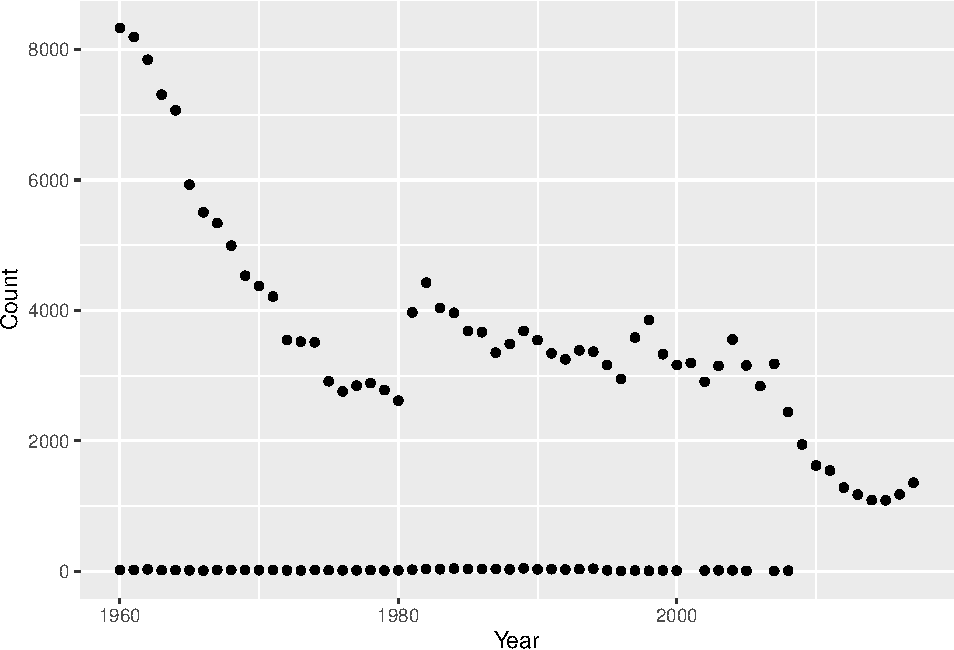
\includegraphics{R/Rintro/figures/unnamed-chunk-31-1.pdf}

Interestingly, there are usually some gender-atypical names, even for
very strongly gendered names like ``Diana''. Splitting these trends out
by \texttt{Sex} is very easy:

\begin{Shaded}
\begin{Highlighting}[]
\KeywordTok{qplot}\NormalTok{(}\DataTypeTok{x =}\NormalTok{ Year, }\DataTypeTok{y =}\NormalTok{ Count, }\DataTypeTok{color =}\NormalTok{ Sex,}
      \DataTypeTok{data =}\NormalTok{ baby_names_diana)}
\end{Highlighting}
\end{Shaded}

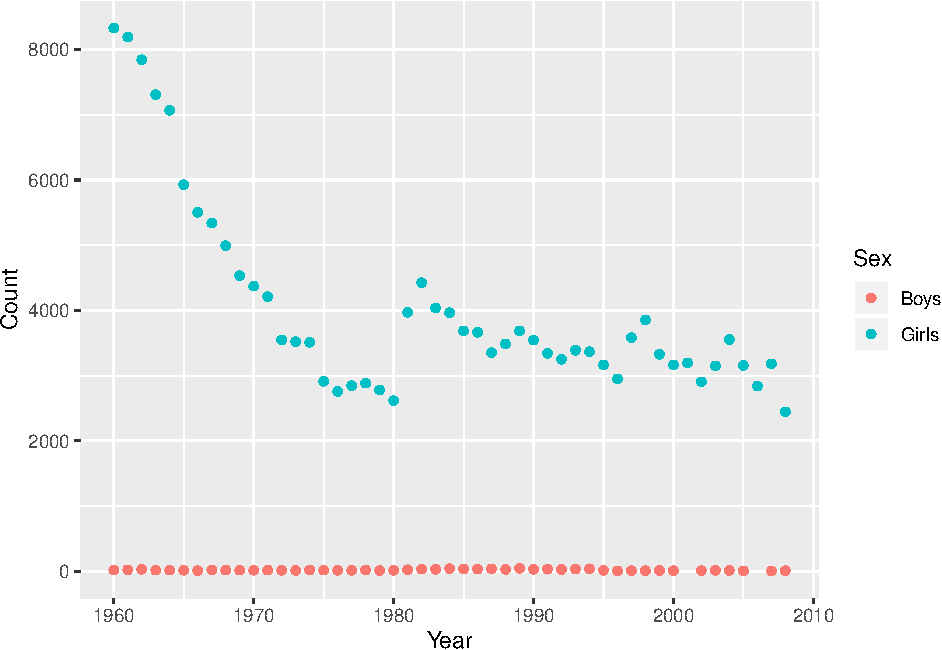
\includegraphics{R/Rintro/figures/unnamed-chunk-32-1.pdf}

\subsection{Exercise 3}\label{exercise-3}

\textbf{Plot peak popularity of your name}

Make sure the \texttt{tidyverse} suite of packages is installed, and
that you have attached them using \texttt{library(tidyverse)}.

\begin{enumerate}
\def\labelenumi{\arabic{enumi}.}
\item
  Use \texttt{filter} to extract data for your name (same as previous
  exercise)

\begin{Shaded}
\begin{Highlighting}[]
\NormalTok{##}
\end{Highlighting}
\end{Shaded}
\item
  Plot the data you produced in step 1 above, with \texttt{Year} on the
  x-axis and \texttt{Count} on the y-axis.

\begin{Shaded}
\begin{Highlighting}[]
\NormalTok{##}
\end{Highlighting}
\end{Shaded}
\item
  Adjust the plot so that is shows boys and girls in different colors.

\begin{Shaded}
\begin{Highlighting}[]
\NormalTok{##}
\end{Highlighting}
\end{Shaded}
\item
  BONUS (Optional): Adjust the plot to use lines instead of points.

\begin{Shaded}
\begin{Highlighting}[]
\NormalTok{##}
\end{Highlighting}
\end{Shaded}
\end{enumerate}

\section{Creating variables}\label{creating-variables}

\textbf{GOAL: To learn how to create new variables with and without
grouped data.} In particular:

\begin{enumerate}
\def\labelenumi{\arabic{enumi}.}
\tightlist
\item
  Creating new variables (columns) --- using the \texttt{mutate()}
  function
\item
  Creating new variables within groups --- by combining the
  \texttt{mutate()} and \texttt{group\_by()} functions
\item
  Recode existing variables --- by combining the \texttt{mutate()} and
  \texttt{case\_when()} functions
\end{enumerate}

We want to use these skills to find out which names have been the most
popular.

\subsection{Create or modify columns}\label{create-or-modify-columns}

So far we've used \texttt{Count} as a measure of popularity. A better
approach is to use proportion to avoid confounding popularity with the
number of babies born in a given year.

The \texttt{mutate()} function makes it easy to add or modify the
columns of a \texttt{data.frame}. For example, we can use it to rescale
the count of each name in each year:

\begin{Shaded}
\begin{Highlighting}[]
\NormalTok{baby_names <-}\StringTok{ }\NormalTok{baby_names }\OperatorTok\StringTok{ }\KeywordTok{mutate}\NormalTok{(}\DataTypeTok{Count_1k =}\NormalTok{ Count}\OperatorTok{/}\DecValTok{1000}\NormalTok{)}
\KeywordTok{head}\NormalTok{(baby_names) }
\end{Highlighting}
\end{Shaded}

\begin{verbatim}
## # A tibble: 6 x 5
##   Name  Sex   Count  Year Count_1k
##   <chr> <chr> <dbl> <dbl>    <dbl>
## 1 Mary  Girls 51474  1960     51.5
## 2 Susan Girls 39200  1960     39.2
## 3 Linda Girls 37314  1960     37.3
## 4 Karen Girls 36376  1960     36.4
## 5 Donna Girls 34133  1960     34.1
## 6 Lisa  Girls 33702  1960     33.7
\end{verbatim}

\subsection{Operating by group}\label{operating-by-group}

Because of the nested nature of our data, we want to compute proportion
or rank \textbf{within} each \texttt{Sex} by \texttt{Year} group. The
\texttt{dplyr} package has a \texttt{group\_by()} function that makes
this relatively straightforward. Here's the logic behind this process:

\begin{figure}
\centering
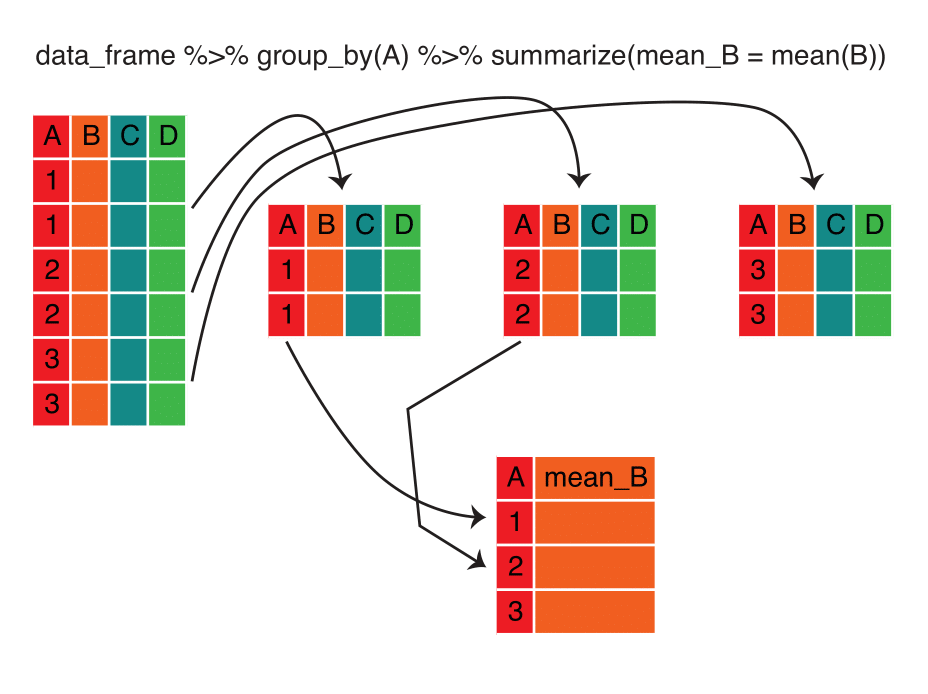
\includegraphics{R/Rintro/images/mutate_group_by.png}
\caption{}
\end{figure}

Note that the \texttt{group\_by()} function converts a \textbf{data
frame} into a \textbf{grouped data frame} --- that is, a data frame with
metadata identifying the groups. The data remain grouped until you
change the groups by running \texttt{group\_by()} again or remove the
grouping metadata using \texttt{ungroup()}.

Here's the code that implements the calculation:

\begin{Shaded}
\begin{Highlighting}[]
\NormalTok{baby_names <-}
\StringTok{  }\NormalTok{baby_names }\OperatorTok
\StringTok{  }\KeywordTok{group_by}\NormalTok{(Year, Sex) }\OperatorTok
\StringTok{  }\KeywordTok{mutate}\NormalTok{(}\DataTypeTok{Rank =} \KeywordTok{rank}\NormalTok{(Count_1k)) }\OperatorTok
\StringTok{  }\KeywordTok{ungroup}\NormalTok{()}

\KeywordTok{head}\NormalTok{(baby_names)}
\end{Highlighting}
\end{Shaded}

\begin{verbatim}
## # A tibble: 6 x 6
##   Name  Sex   Count  Year Count_1k  Rank
##   <chr> <chr> <dbl> <dbl>    <dbl> <dbl>
## 1 Mary  Girls 51474  1960     51.5  7331
## 2 Susan Girls 39200  1960     39.2  7330
## 3 Linda Girls 37314  1960     37.3  7329
## 4 Karen Girls 36376  1960     36.4  7328
## 5 Donna Girls 34133  1960     34.1  7327
## 6 Lisa  Girls 33702  1960     33.7  7326
\end{verbatim}

\subsection{Recoding variables}\label{recoding-variables}

It's often necessary to create a new variable that is a recoded version
of an existing variable. For example, we might want to take our
\texttt{Count\_1k} variable and create a new variable that divides it
into \texttt{low}, \texttt{medium}, and \texttt{high} categories. To do
this, we can use the \texttt{case\_when()} function within the
\texttt{mutate()} function:

\begin{Shaded}
\begin{Highlighting}[]
\NormalTok{baby_names <-}
\StringTok{  }\NormalTok{baby_names }\OperatorTok
\StringTok{  }\KeywordTok{mutate}\NormalTok{(}\DataTypeTok{Count_levels =} \KeywordTok{case_when}\NormalTok{(}
\NormalTok{                            Count_1k }\OperatorTok{<=}\StringTok{ }\DecValTok{10}                  \OperatorTok{~}\StringTok{ "low"}\NormalTok{,}
\NormalTok{                            Count_1k  }\OperatorTok{>}\StringTok{ }\DecValTok{10} \OperatorTok{&}\StringTok{ }\NormalTok{Count_1k }\OperatorTok{<=}\StringTok{ }\DecValTok{40} \OperatorTok{~}\StringTok{ "medium"}\NormalTok{,}
\NormalTok{                            Count_1k  }\OperatorTok{>}\StringTok{ }\DecValTok{40}                  \OperatorTok{~}\StringTok{ "high"}
\NormalTok{                            ))}

\KeywordTok{head}\NormalTok{(baby_names)                            }
\end{Highlighting}
\end{Shaded}

\begin{verbatim}
## # A tibble: 6 x 7
##   Name  Sex   Count  Year Count_1k  Rank Count_levels
##   <chr> <chr> <dbl> <dbl>    <dbl> <dbl> <chr>       
## 1 Mary  Girls 51474  1960     51.5  7331 high        
## 2 Susan Girls 39200  1960     39.2  7330 medium      
## 3 Linda Girls 37314  1960     37.3  7329 medium      
## 4 Karen Girls 36376  1960     36.4  7328 medium      
## 5 Donna Girls 34133  1960     34.1  7327 medium      
## 6 Lisa  Girls 33702  1960     33.7  7326 medium
\end{verbatim}

\subsection{Exercise 4}\label{exercise-4}

\textbf{Most popular names}

In this exercise your goal is to identify the most popular names for
each year.

\begin{enumerate}
\def\labelenumi{\arabic{enumi}.}
\item
  Use \texttt{mutate()} and \texttt{group\_by()} to create a column
  named \texttt{Proportion} where
  \texttt{Proportion\ =\ Count/sum(Count)} for each
  \texttt{Year\ X\ Sex} group. Use pipes wherever it makes sense.

\begin{Shaded}
\begin{Highlighting}[]
\NormalTok{##}
\end{Highlighting}
\end{Shaded}
\item
  Use \texttt{mutate()} and \texttt{group\_by()} to create a column
  named \texttt{Rank} where \texttt{Rank\ =\ rank(desc(Count))} for each
  \texttt{Year\ X\ Sex} group.

\begin{Shaded}
\begin{Highlighting}[]
\NormalTok{##}
\end{Highlighting}
\end{Shaded}
\item
  Filter the baby names data to display only the most popular name for
  each \texttt{Year\ X\ Sex} group. Keep only the columns:
  \texttt{Year}, \texttt{Name}, \texttt{Sex}, and \texttt{Proportion}.

\begin{Shaded}
\begin{Highlighting}[]
\NormalTok{##}
\end{Highlighting}
\end{Shaded}
\item
  Plot the data produced in step 3, putting \texttt{Year} on the x-axis
  and \texttt{Proportion} on the y-axis. How has the proportion of
  babies given the most popular name changed over time?

\begin{Shaded}
\begin{Highlighting}[]
\NormalTok{##}
\end{Highlighting}
\end{Shaded}
\item
  BONUS (optional): Which names are the most popular for both boys and
  girls?

\begin{Shaded}
\begin{Highlighting}[]
\NormalTok{##}
\end{Highlighting}
\end{Shaded}
\end{enumerate}

\section{Aggregating variables}\label{aggregating-variables}

\textbf{GOAL: To learn how to aggregate data to create summaries with
and without grouped data.} In particular:

\begin{enumerate}
\def\labelenumi{\arabic{enumi}.}
\tightlist
\item
  Collapsing data into summaries --- using the \texttt{summarize()}
  function
\item
  Creating summaries within groups --- by combining the
  \texttt{summarize()} and \texttt{group\_by()} functions
\end{enumerate}

You may have noticed that the percentage of babies given the most
popular name of the year appears to have decreased over time. We can
compute a more robust measure of the popularity of the most popular
names by calculating the number of babies given one of the top 10 girl
or boy names of the year.

To compute this measure we need to operate within groups, as we did
using \texttt{mutate()} above, but this time we need to collapse each
group into a single summary statistic. We can achieve this using the
\texttt{summarize()} function.

First, let's see how this function works without grouping. The following
code outputs the total number of girls and boys in the data:

\begin{Shaded}
\begin{Highlighting}[]
\NormalTok{baby_names }\OperatorTok\StringTok{ }
\StringTok{  }\KeywordTok{summarize}\NormalTok{(}\DataTypeTok{Girls_n =} \KeywordTok{sum}\NormalTok{(Sex}\OperatorTok{==}\StringTok{"Girls"}\NormalTok{),}
            \DataTypeTok{Boys_n =} \KeywordTok{sum}\NormalTok{(Sex}\OperatorTok{==}\StringTok{"Boys"}\NormalTok{))}
\end{Highlighting}
\end{Shaded}

\begin{verbatim}
## # A tibble: 1 x 2
##   Girls_n Boys_n
##     <int>  <int>
## 1  641084 407491
\end{verbatim}

Next, using \texttt{group\_by()} and \texttt{summarize()} together, we
can calculate the number of babies born each year. Here's the logic
behind this process:

\begin{figure}
\centering
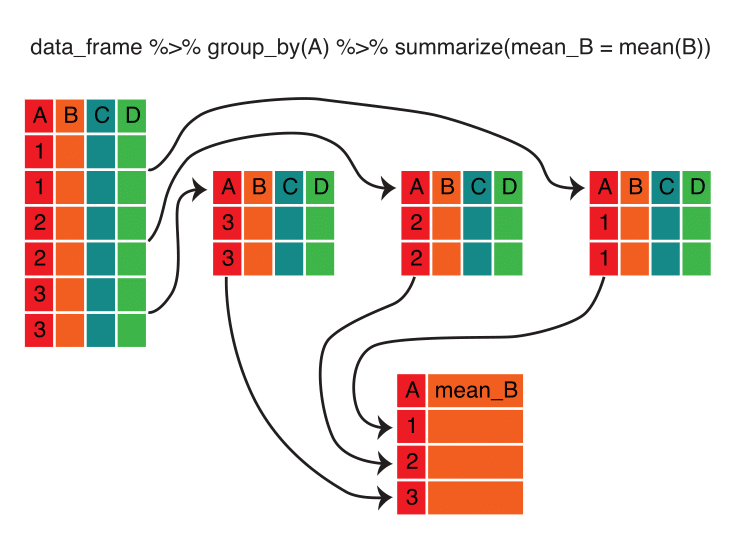
\includegraphics{R/Rintro/images/summarize_group_by.png}
\caption{}
\end{figure}

Note that, unlike with the \texttt{mutate()} function, the
\texttt{summarize()} function returns a data frame with fewer rows than
the original, because of aggregation.

Here's the code that implements the calculation:

\begin{Shaded}
\begin{Highlighting}[]
\NormalTok{bn_by_year <-}
\StringTok{  }\NormalTok{baby_names }\OperatorTok
\StringTok{  }\KeywordTok{group_by}\NormalTok{(Year) }\OperatorTok
\StringTok{  }\KeywordTok{summarize}\NormalTok{(}\DataTypeTok{Total =} \KeywordTok{sum}\NormalTok{(Count)) }\OperatorTok
\StringTok{  }\KeywordTok{ungroup}\NormalTok{()}

\KeywordTok{head}\NormalTok{(bn_by_year)}
\end{Highlighting}
\end{Shaded}

\begin{verbatim}
## # A tibble: 6 x 2
##    Year   Total
##   <dbl>   <dbl>
## 1  1960 4154377
## 2  1961 4140244
## 3  1962 4035234
## 4  1963 3958791
## 5  1964 3887800
## 6  1965 3626029
\end{verbatim}

\subsection{Exercise 5}\label{exercise-5}

\textbf{Popularity of the most popular names}

In this exercise we will plot trends in the proportion of boys and girls
given one of the 10 most popular names each year.

\begin{enumerate}
\def\labelenumi{\arabic{enumi}.}
\item
  Filter the \texttt{baby\_names} data, retaining only the 10 most
  popular girl and boy names for each year.

\begin{Shaded}
\begin{Highlighting}[]
\NormalTok{##}
\end{Highlighting}
\end{Shaded}
\item
  Summarize the data produced in step one to calculate the total
  Proportion of boys and girls given one of the top 10 names each year.

\begin{Shaded}
\begin{Highlighting}[]
\NormalTok{##}
\end{Highlighting}
\end{Shaded}
\item
  Plot the data produced in step 2, with year on the x-axis and total
  proportion on the y axis. Color by \texttt{Sex} and notice the trend.

\begin{Shaded}
\begin{Highlighting}[]
\NormalTok{##}
\end{Highlighting}
\end{Shaded}
\end{enumerate}

\section{Saving work}\label{saving-work}

\textbf{GOAL: To learn how to save objects, data, and scripts for later
use.}

Now that we have made some changes to our data set, we might want to
save those changes to a file.

\subsection{Saving individual
datasets}\label{saving-individual-datasets}

You might find functions \texttt{write\_csv()} and \texttt{write\_rds()}
from package \texttt{readr} handy!

\begin{Shaded}
\begin{Highlighting}[]
\CommentTok{# write data to a .csv file}
\KeywordTok{write_csv}\NormalTok{(baby_names, }\StringTok{"babyNames.csv"}\NormalTok{)}
\end{Highlighting}
\end{Shaded}

\begin{Shaded}
\begin{Highlighting}[]
\CommentTok{# write data to an R file}
\KeywordTok{write_rds}\NormalTok{(baby_names, }\StringTok{"babyNames.rds"}\NormalTok{)}
\end{Highlighting}
\end{Shaded}

\subsection{Saving multiple datasets}\label{saving-multiple-datasets}

\begin{Shaded}
\begin{Highlighting}[]
\KeywordTok{ls}\NormalTok{() }\CommentTok{# list objects in our workspace}
\KeywordTok{save}\NormalTok{(baby_names_diana, bn_by_year, baby_names_subset, }\DataTypeTok{file=}\StringTok{"myDataFiles.RData"}\NormalTok{)  }
\end{Highlighting}
\end{Shaded}

\begin{Shaded}
\begin{Highlighting}[]
\NormalTok{## Load the "myDataFiles.RData"}
\NormalTok{## load("myDataFiles.RData") }
\end{Highlighting}
\end{Shaded}

\subsection{Saving \& loading
workspaces}\label{saving-loading-workspaces}

In addition to importing individual datasets, R can save and load entire
``workspaces''. The workspace is your current R working environment and
includes any user-defined objects. At the end of a session, you can save
an ``image'' of the current workspace, which allows you to automatically
reload the objects you previously created.

\begin{Shaded}
\begin{Highlighting}[]
\KeywordTok{ls}\NormalTok{() }\CommentTok{# list objects in our workspace}
\KeywordTok{save.image}\NormalTok{(}\DataTypeTok{file=}\StringTok{"myWorkspace.RData"}\NormalTok{) }\CommentTok{# save workspace }
\KeywordTok{rm}\NormalTok{(}\DataTypeTok{list=}\KeywordTok{ls}\NormalTok{()) }\CommentTok{# remove all objects from our workspace }
\KeywordTok{ls}\NormalTok{() }\CommentTok{# list stored objects to make sure they are deleted}
\end{Highlighting}
\end{Shaded}

\begin{Shaded}
\begin{Highlighting}[]
\NormalTok{## Load the "myWorkspace.RData" file and check that it is restored}
\KeywordTok{load}\NormalTok{(}\StringTok{"myWorkspace.RData"}\NormalTok{) }\CommentTok{# load myWorkspace.RData}
\KeywordTok{ls}\NormalTok{() }\CommentTok{# list objects}
\end{Highlighting}
\end{Shaded}

\section{Exercise solutions}\label{exercise-solutions}

\subsection{Ex 0: prototype}\label{ex-0-prototype}

\begin{enumerate}
\def\labelenumi{\arabic{enumi}.}
\item
  2 plus 2

\begin{Shaded}
\begin{Highlighting}[]
\DecValTok{2} \OperatorTok{+}\StringTok{ }\DecValTok{2}
\end{Highlighting}
\end{Shaded}

\begin{verbatim}
## [1] 4
\end{verbatim}

\begin{Shaded}
\begin{Highlighting}[]
\CommentTok{# or}
\KeywordTok{sum}\NormalTok{(}\DecValTok{2}\NormalTok{, }\DecValTok{2}\NormalTok{)}
\end{Highlighting}
\end{Shaded}

\begin{verbatim}
## [1] 4
\end{verbatim}
\item
  square root of 10

\begin{Shaded}
\begin{Highlighting}[]
\KeywordTok{sqrt}\NormalTok{(}\DecValTok{10}\NormalTok{)}
\end{Highlighting}
\end{Shaded}

\begin{verbatim}
## [1] 3.16228
\end{verbatim}

\begin{Shaded}
\begin{Highlighting}[]
\CommentTok{# or}
\DecValTok{10}\OperatorTok{^}\NormalTok{(}\DecValTok{1}\OperatorTok{/}\DecValTok{2}\NormalTok{)}
\end{Highlighting}
\end{Shaded}

\begin{verbatim}
## [1] 3.16228
\end{verbatim}
\item
  Find ``An Introduction to R''.

\begin{Shaded}
\begin{Highlighting}[]
\CommentTok{# Go to the main help page by running 'help.start() or using the GUI}
\CommentTok{# menu, find and click on the link to "An Introduction to R".}
\end{Highlighting}
\end{Shaded}
\end{enumerate}

\subsection{Ex 1: prototype}\label{ex-1-prototype}

\begin{enumerate}
\def\labelenumi{\arabic{enumi}.}
\item
  Open the \texttt{read\_csv()} help page to determine how to use it to
  read in data.

\begin{Shaded}
\begin{Highlighting}[]
\NormalTok{?read_csv}
\end{Highlighting}
\end{Shaded}
\item
  Read the baby names data using the \texttt{read\_csv()} function and
  assign the result with the name \texttt{baby\_names}.

\begin{Shaded}
\begin{Highlighting}[]
\NormalTok{baby_names <-}\StringTok{ }\KeywordTok{read_csv}\NormalTok{(}\StringTok{"babyNames.csv"}\NormalTok{)}
\end{Highlighting}
\end{Shaded}
\item
  BONUS (optional): Save the \texttt{baby\_names} data as a Stata data
  set \texttt{babynames.dta} and as an R data set
  \texttt{babynames.rds}.

\begin{Shaded}
\begin{Highlighting}[]
\KeywordTok{write_dta}\NormalTok{(baby_names, }\DataTypeTok{version =} \DecValTok{15}\NormalTok{, }\DataTypeTok{path =}\NormalTok{ “babynames.dta”)}

\KeywordTok{write_rds}\NormalTok{(baby_names, }\DataTypeTok{file =}\NormalTok{ “babynames.rds”)}
\end{Highlighting}
\end{Shaded}
\end{enumerate}

\subsection{Ex 2.1: prototype}\label{ex-2.1-prototype}

\begin{enumerate}
\def\labelenumi{\arabic{enumi}.}
\item
  Use \texttt{filter} to extract data for your name (or another name of
  your choice).

\begin{Shaded}
\begin{Highlighting}[]
\NormalTok{baby_names_george <-}\StringTok{ }\KeywordTok{filter}\NormalTok{(baby_names, Name }\OperatorTok{==}\StringTok{ "George"}\NormalTok{)}
\end{Highlighting}
\end{Shaded}
\item
  Arrange the data you produced in step 1 above by \texttt{Count}. In
  which year was the name most popular?

\begin{Shaded}
\begin{Highlighting}[]
\KeywordTok{arrange}\NormalTok{(baby_names_george, }\KeywordTok{desc}\NormalTok{(Count))}
\end{Highlighting}
\end{Shaded}

\begin{verbatim}
## # A tibble: 97 x 4
##    Name   Sex   Count  Year
##    <chr>  <chr> <dbl> <dbl>
##  1 George Boys  14063  1960
##  2 George Boys  13638  1961
##  3 George Boys  12553  1962
##  4 George Boys  12084  1963
##  5 George Boys  11793  1964
##  6 George Boys  10683  1965
##  7 George Boys   9942  1966
##  8 George Boys   9702  1967
##  9 George Boys   9388  1968
## 10 George Boys   9203  1969
## # ... with 87 more rows
\end{verbatim}
\item
  BONUS (optional): Filter the data to extract \emph{only} the row
  containing the most popular boys name in 1999.

\begin{Shaded}
\begin{Highlighting}[]
\NormalTok{baby_names_boys_}\DecValTok{1999}\NormalTok{ <-}\StringTok{ }\KeywordTok{filter}\NormalTok{(baby_names,}
\NormalTok{                               Year }\OperatorTok{==}\StringTok{ }\DecValTok{1999} \OperatorTok{&}\StringTok{ }\NormalTok{Sex }\OperatorTok{==}\StringTok{ "Boys"}\NormalTok{)}
\end{Highlighting}
\end{Shaded}

\begin{Shaded}
\begin{Highlighting}[]
\KeywordTok{filter}\NormalTok{(baby_names_boys_}\DecValTok{1999}\NormalTok{, Count }\OperatorTok{==}\StringTok{ }\KeywordTok{max}\NormalTok{(Count))}
\end{Highlighting}
\end{Shaded}

\begin{verbatim}
## # A tibble: 1 x 4
##   Name  Sex   Count  Year
##   <chr> <chr> <dbl> <dbl>
## 1 Jacob Boys  35361  1999
\end{verbatim}
\end{enumerate}

\subsection{Ex 2.2: prototype}\label{ex-2.2-prototype}

Rewrite the solution to Exercise 2.1 using pipes.

\begin{Shaded}
\begin{Highlighting}[]
\NormalTok{baby_names }\OperatorTok\StringTok{ }
\StringTok{    }\KeywordTok{filter}\NormalTok{(Name }\OperatorTok{==}\StringTok{ "George"}\NormalTok{) }\OperatorTok
\StringTok{    }\KeywordTok{arrange}\NormalTok{(}\KeywordTok{desc}\NormalTok{(Count))}
\end{Highlighting}
\end{Shaded}

\begin{verbatim}
## # A tibble: 97 x 4
##    Name   Sex   Count  Year
##    <chr>  <chr> <dbl> <dbl>
##  1 George Boys  14063  1960
##  2 George Boys  13638  1961
##  3 George Boys  12553  1962
##  4 George Boys  12084  1963
##  5 George Boys  11793  1964
##  6 George Boys  10683  1965
##  7 George Boys   9942  1966
##  8 George Boys   9702  1967
##  9 George Boys   9388  1968
## 10 George Boys   9203  1969
## # ... with 87 more rows
\end{verbatim}

\subsection{Ex 3: prototype}\label{ex-3-prototype}

\begin{enumerate}
\def\labelenumi{\arabic{enumi}.}
\item
  Use \texttt{filter()} to extract data for your name (same as previous
  exercise).

\begin{Shaded}
\begin{Highlighting}[]
\NormalTok{baby_names_george <-}\StringTok{ }\KeywordTok{filter}\NormalTok{(baby_names, Name }\OperatorTok{==}\StringTok{ "George"}\NormalTok{)}
\end{Highlighting}
\end{Shaded}
\item
  Plot the data you produced in step 1 above, with \texttt{Year} on the
  x-axis and \texttt{Count} on the y-axis.

\begin{Shaded}
\begin{Highlighting}[]
\KeywordTok{qplot}\NormalTok{(}\DataTypeTok{x =}\NormalTok{ Year, }\DataTypeTok{y =}\NormalTok{ Count, }\DataTypeTok{data =}\NormalTok{ baby_names_george)}
\end{Highlighting}
\end{Shaded}

  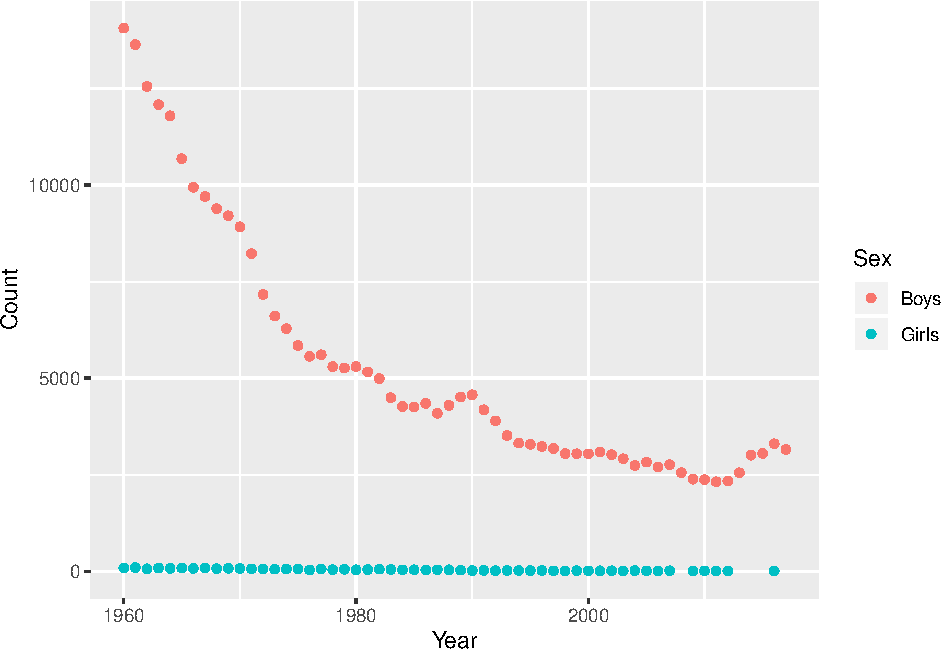
\includegraphics{R/Rintro/figures/unnamed-chunk-68-1.pdf}
\item
  Adjust the plot so that is shows boys and girls in different colors.

\begin{Shaded}
\begin{Highlighting}[]
\KeywordTok{qplot}\NormalTok{(}\DataTypeTok{x =}\NormalTok{ Year, }\DataTypeTok{y =}\NormalTok{ Count, }\DataTypeTok{color =}\NormalTok{ Sex, }\DataTypeTok{data =}\NormalTok{ baby_names_george)}
\end{Highlighting}
\end{Shaded}

  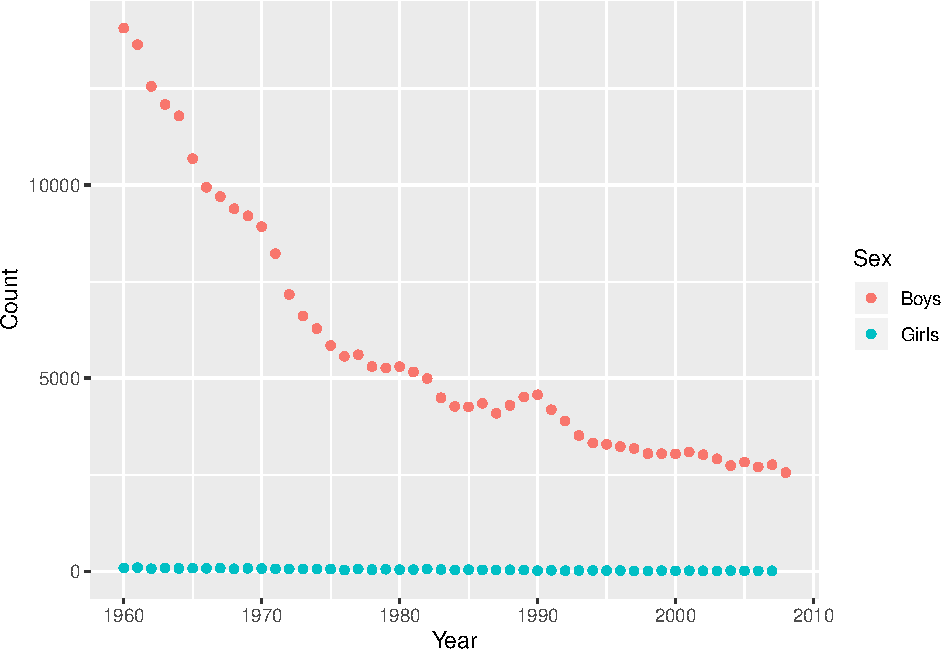
\includegraphics{R/Rintro/figures/unnamed-chunk-69-1.pdf}
\item
  BONUS (Optional): Adjust the plot to use lines instead of points.

\begin{Shaded}
\begin{Highlighting}[]
\KeywordTok{qplot}\NormalTok{(}\DataTypeTok{x =}\NormalTok{ Year, }\DataTypeTok{y =}\NormalTok{ Count, }\DataTypeTok{color =}\NormalTok{ Sex, }\DataTypeTok{data =}\NormalTok{ baby_names_george, }\DataTypeTok{geom =} \StringTok{"line"}\NormalTok{)}
\end{Highlighting}
\end{Shaded}

  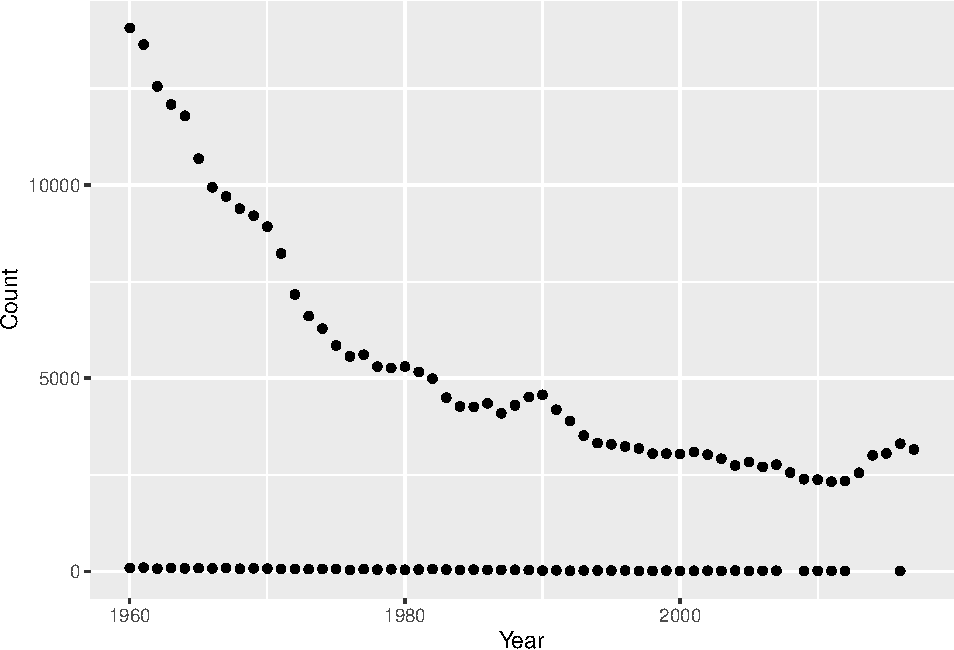
\includegraphics{R/Rintro/figures/unnamed-chunk-70-1.pdf}
\end{enumerate}

\subsection{Ex 4: prototype}\label{ex-4-prototype}

\begin{enumerate}
\def\labelenumi{\arabic{enumi}.}
\item
  Use \texttt{mutate()} and \texttt{group\_by()} to create a column
  named \texttt{Proportion} where
  \texttt{Proportion\ =\ Count/sum(Count)} for each
  \texttt{Year\ X\ Sex} group.

\begin{Shaded}
\begin{Highlighting}[]
\NormalTok{baby_names <-}\StringTok{ }
\StringTok{  }\NormalTok{baby_names }\OperatorTok
\StringTok{  }\KeywordTok{group_by}\NormalTok{(Year, Sex) }\OperatorTok
\StringTok{  }\KeywordTok{mutate}\NormalTok{(}\DataTypeTok{Proportion =}\NormalTok{ Count}\OperatorTok{/}\KeywordTok{sum}\NormalTok{(Count)) }\OperatorTok
\StringTok{  }\KeywordTok{ungroup}\NormalTok{()}

\KeywordTok{head}\NormalTok{(baby_names) }
\end{Highlighting}
\end{Shaded}

\begin{verbatim}
## # A tibble: 6 x 5
##   Name  Sex   Count  Year Proportion
##   <chr> <chr> <dbl> <dbl>      <dbl>
## 1 Mary  Girls 51474  1960     0.0255
## 2 Susan Girls 39200  1960     0.0194
## 3 Linda Girls 37314  1960     0.0185
## 4 Karen Girls 36376  1960     0.0180
## 5 Donna Girls 34133  1960     0.0169
## 6 Lisa  Girls 33702  1960     0.0167
\end{verbatim}
\item
  Use \texttt{mutate()} and \texttt{group\_by()} to create a column
  named \texttt{Rank} where \texttt{Rank\ =\ rank(desc(Count))} for each
  \texttt{Year\ X\ Sex} group.

\begin{Shaded}
\begin{Highlighting}[]
\NormalTok{baby_names <-}\StringTok{ }
\StringTok{  }\NormalTok{baby_names }\OperatorTok
\StringTok{  }\KeywordTok{group_by}\NormalTok{(Year, Sex) }\OperatorTok
\StringTok{  }\KeywordTok{mutate}\NormalTok{(}\DataTypeTok{Rank =} \KeywordTok{rank}\NormalTok{(}\KeywordTok{desc}\NormalTok{(Count))) }\OperatorTok
\StringTok{  }\KeywordTok{ungroup}\NormalTok{()}

\KeywordTok{head}\NormalTok{(baby_names)}
\end{Highlighting}
\end{Shaded}

\begin{verbatim}
## # A tibble: 6 x 6
##   Name  Sex   Count  Year Proportion  Rank
##   <chr> <chr> <dbl> <dbl>      <dbl> <dbl>
## 1 Mary  Girls 51474  1960     0.0255     1
## 2 Susan Girls 39200  1960     0.0194     2
## 3 Linda Girls 37314  1960     0.0185     3
## 4 Karen Girls 36376  1960     0.0180     4
## 5 Donna Girls 34133  1960     0.0169     5
## 6 Lisa  Girls 33702  1960     0.0167     6
\end{verbatim}
\item
  Filter the baby names data to display only the most popular name for
  each \texttt{Year\ X\ Sex} group.

\begin{Shaded}
\begin{Highlighting}[]
\NormalTok{top1 <-}\StringTok{ }
\StringTok{  }\NormalTok{baby_names }\OperatorTok
\StringTok{  }\KeywordTok{filter}\NormalTok{(Rank }\OperatorTok{==}\StringTok{ }\DecValTok{1}\NormalTok{) }\OperatorTok
\StringTok{  }\KeywordTok{select}\NormalTok{(Year, Name, Sex, Proportion)}

\KeywordTok{head}\NormalTok{(top1)}
\end{Highlighting}
\end{Shaded}

\begin{verbatim}
## # A tibble: 6 x 4
##    Year Name    Sex   Proportion
##   <dbl> <chr>   <chr>      <dbl>
## 1  1960 Mary    Girls     0.0255
## 2  1960 David   Boys      0.0403
## 3  1961 Mary    Girls     0.0236
## 4  1961 Michael Boys      0.0409
## 5  1962 Lisa    Girls     0.0234
## 6  1962 Michael Boys      0.0411
\end{verbatim}
\item
  Plot the data produced in step 3, putting \texttt{Year} on the x-axis
  and \texttt{Proportion} on the y-axis. How has the proportion of
  babies given the most popular name changed over time?

\begin{Shaded}
\begin{Highlighting}[]
\KeywordTok{qplot}\NormalTok{(}\DataTypeTok{x =}\NormalTok{ Year, }
      \DataTypeTok{y =}\NormalTok{ Proportion, }
      \DataTypeTok{color =}\NormalTok{ Sex, }
      \DataTypeTok{data =}\NormalTok{ top1, }
      \DataTypeTok{geom =} \StringTok{"line"}\NormalTok{)}
\end{Highlighting}
\end{Shaded}

  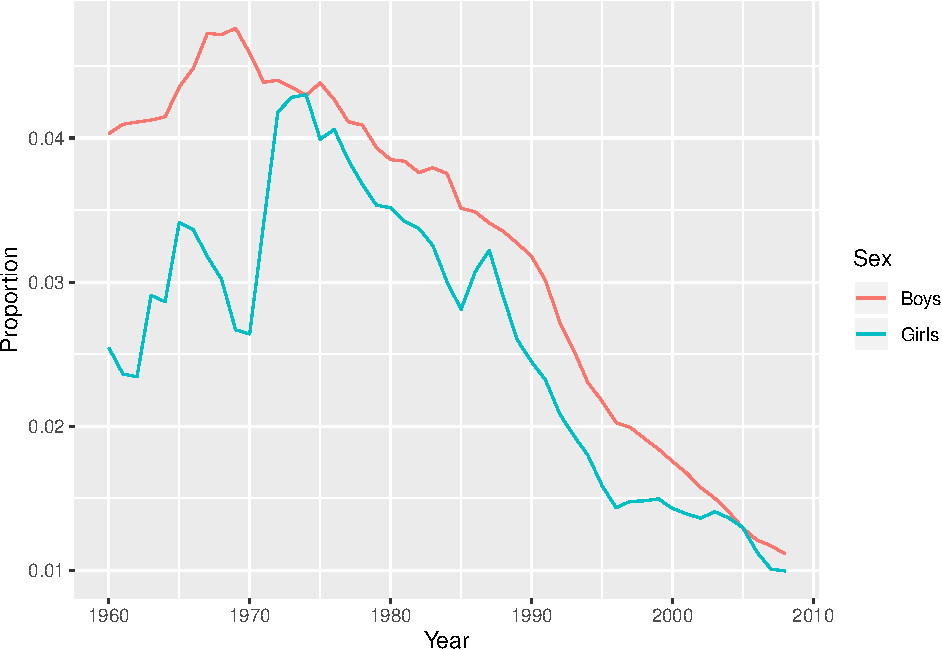
\includegraphics{R/Rintro/figures/unnamed-chunk-74-1.pdf}
\item
  BONUS (optional): Which names are the most popular for both boys and
  girls?

\begin{Shaded}
\begin{Highlighting}[]
\NormalTok{girls_and_boys <-}\StringTok{ }\KeywordTok{inner_join}\NormalTok{(}\KeywordTok{filter}\NormalTok{(baby_names, Sex }\OperatorTok{==}\StringTok{ "Boys"}\NormalTok{), }
                            \KeywordTok{filter}\NormalTok{(baby_names, Sex }\OperatorTok{==}\StringTok{ "Girls"}\NormalTok{),}
                            \DataTypeTok{by =} \KeywordTok{c}\NormalTok{(}\StringTok{"Year"}\NormalTok{, }\StringTok{"Name"}\NormalTok{))}

\NormalTok{girls_and_boys <-}\StringTok{ }\KeywordTok{mutate}\NormalTok{(girls_and_boys,}
                        \DataTypeTok{Product =}\NormalTok{ Count.x }\OperatorTok{*}\StringTok{ }\NormalTok{Count.y,}
                        \DataTypeTok{Rank =} \KeywordTok{rank}\NormalTok{(}\KeywordTok{desc}\NormalTok{(Product)))}

\KeywordTok{filter}\NormalTok{(girls_and_boys, Rank }\OperatorTok{==}\StringTok{ }\DecValTok{1}\NormalTok{)}
\end{Highlighting}
\end{Shaded}

\begin{verbatim}
## # A tibble: 1 x 12
##   Name   Sex.x Count.x  Year Proportion.x Rank.x Sex.y Count.y Proportion.y Rank.y   Product  Rank
##   <chr>  <chr>   <dbl> <dbl>        <dbl>  <dbl> <chr>   <dbl>        <dbl>  <dbl>     <dbl> <dbl>
## 1 Taylor Boys     7688  1993      0.00392     51 Girls   21266       0.0118      7 163493008     1
\end{verbatim}
\end{enumerate}

\subsection{Ex 5: prototype}\label{ex-5-prototype}

\begin{enumerate}
\def\labelenumi{\arabic{enumi}.}
\item
  Filter the baby\_names data, retaining only the 10 most popular girl
  and boy names for each year.

\begin{Shaded}
\begin{Highlighting}[]
\NormalTok{most_popular <-}\StringTok{ }
\StringTok{  }\NormalTok{baby_names }\OperatorTok\StringTok{ }
\StringTok{  }\KeywordTok{group_by}\NormalTok{(Year, Sex) }\OperatorTok
\StringTok{  }\KeywordTok{filter}\NormalTok{(Rank }\OperatorTok{<=}\StringTok{ }\DecValTok{10}\NormalTok{)}

\KeywordTok{head}\NormalTok{(most_popular, }\DataTypeTok{n =} \DecValTok{10}\NormalTok{)}
\end{Highlighting}
\end{Shaded}

\begin{verbatim}
## # A tibble: 10 x 6
## # Groups:   Year, Sex [1]
##    Name     Sex   Count  Year Proportion  Rank
##    <chr>    <chr> <dbl> <dbl>      <dbl> <dbl>
##  1 Mary     Girls 51474  1960     0.0255     1
##  2 Susan    Girls 39200  1960     0.0194     2
##  3 Linda    Girls 37314  1960     0.0185     3
##  4 Karen    Girls 36376  1960     0.0180     4
##  5 Donna    Girls 34133  1960     0.0169     5
##  6 Lisa     Girls 33702  1960     0.0167     6
##  7 Patricia Girls 32102  1960     0.0159     7
##  8 Debra    Girls 26737  1960     0.0132     8
##  9 Cynthia  Girls 26725  1960     0.0132     9
## 10 Deborah  Girls 25264  1960     0.0125    10
\end{verbatim}
\item
  Summarize the data produced in step one to calculate the total
  Proportion of boys and girls given one of the top 10 names each year.

\begin{Shaded}
\begin{Highlighting}[]
\NormalTok{top10 <-}\StringTok{ }
\StringTok{  }\NormalTok{most_popular }\OperatorTok\StringTok{ }\CommentTok{# it is already grouped by Year and Sex}
\StringTok{  }\KeywordTok{summarize}\NormalTok{(}\DataTypeTok{TotalProportion =} \KeywordTok{sum}\NormalTok{(Proportion))}
\end{Highlighting}
\end{Shaded}
\item
  Plot the data produced in step 2, with year on the x-axis and total
  proportion on the y axis. Color by \texttt{Sex}.

\begin{Shaded}
\begin{Highlighting}[]
\KeywordTok{qplot}\NormalTok{(}\DataTypeTok{x =}\NormalTok{ Year, }
      \DataTypeTok{y =}\NormalTok{ TotalProportion, }
      \DataTypeTok{color =}\NormalTok{ Sex,}
      \DataTypeTok{data =}\NormalTok{ top10,}
      \DataTypeTok{geom =} \StringTok{"line"}\NormalTok{)}
\end{Highlighting}
\end{Shaded}

  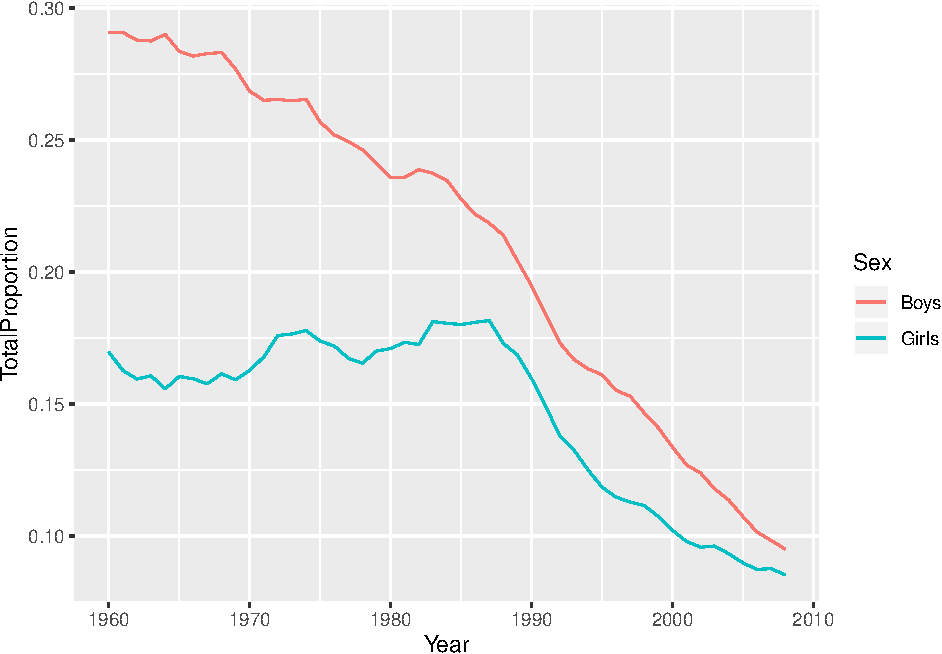
\includegraphics{R/Rintro/figures/unnamed-chunk-78-1.pdf}
\end{enumerate}

\section{Wrap-up}\label{wrap-up-1}

\subsection{Feedback}\label{feedback-1}

These workshops are a work-in-progress, please provide any feedback to:
\href{mailto:help@iq.harvard.edu}{\nolinkurl{help@iq.harvard.edu}}

\subsection{Resources}\label{resources-2}

\begin{itemize}
\tightlist
\item
  IQSS

  \begin{itemize}
  \tightlist
  \item
    Workshops: \url{https://dss.iq.harvard.edu/workshop-materials}
  \item
    Data Science Services: \url{https://dss.iq.harvard.edu/}
  \item
    Research Computing Environment:
    \url{https://iqss.github.io/dss-rce/}
  \end{itemize}
\item
  HBS

  \begin{itemize}
  \tightlist
  \item
    Research Computing Services workshops:
    \url{https://training.rcs.hbs.org/workshops}
  \item
    Other HBS RCS resources:
    \url{https://training.rcs.hbs.org/workshop-materials}
  \item
    RCS consulting email: \url{mailto:research@hbs.edu}
  \end{itemize}
\item
  Software (all free!):

  \begin{itemize}
  \tightlist
  \item
    R and R package download: \url{http://cran.r-project.org}
  \item
    Rstudio download: \url{http://rstudio.org}
  \item
    ESS (emacs R package): \url{http://ess.r-project.org/}
  \end{itemize}
\item
  Cheatsheets

  \begin{itemize}
  \tightlist
  \item
    \url{https://rstudio.com/wp-content/uploads/2019/01/Cheatsheets_2019.pdf}
  \end{itemize}
\item
  Online tutorials

  \begin{itemize}
  \tightlist
  \item
    \url{https://swirlstats.com/}
  \item
    \url{https://r4ds.had.co.nz/}
  \item
    \url{https://hbs-rcs.github.io/R_Intro-gapminder/base-r/}
  \item
    \url{https://www.pluralsight.com/search?q=R}
  \item
    \url{https://www.datacamp.com/}
  \item
    \url{https://rmarkdown.rstudio.com/lesson-1.html}
  \end{itemize}
\item
  Getting help:

  \begin{itemize}
  \tightlist
  \item
    Documentation and tutorials:
    \url{http://cran.r-project.org/other-docs.html}
  \item
    Recommended R packages by topic:
    \url{http://cran.r-project.org/web/views/}
  \item
    Mailing list: \url{https://stat.ethz.ch/mailman/listinfo/r-help}
  \item
    StackOverflow: \url{http://stackoverflow.com/questions/tagged/r}
  \item
    R-Bloggers: \url{https://www.r-bloggers.com/}
  \end{itemize}
\item
  Coming from \ldots{}

  \begin{itemize}
  \tightlist
  \item
    Stata: \url{http://www.princeton.edu/~otorres/RStata.pdf}
  \item
    SAS/SPSS: \url{http://r4stats.com/books/free-version/}
  \item
    Matlab: \url{http://www.math.umaine.edu/~hiebeler/comp/matlabR.pdf}
  \item
    Python:
    \url{http://mathesaurus.sourceforge.net/matlab-python-xref.pdf}
  \end{itemize}
\end{itemize}

\chapter{R Regression Models}\label{r-regression-models}

\textbf{Topics}

\begin{itemize}
\tightlist
\item
  Formula interface for model specification
\item
  Function methods for extracting quantities of interest from models
\item
  Contrasts to test specific hypotheses
\item
  Model comparisons
\item
  Predicted marginal effects
\end{itemize}

\section{Setup}\label{setup-1}

\subsection{Class Structure}\label{class-structure-1}

\begin{itemize}
\tightlist
\item
  Informal --- Ask questions at any time. Really!
\item
  Collaboration is encouraged - please spend a minute introducing
  yourself to your neighbors!
\end{itemize}

\subsection{Prerequisites}\label{prerequisites-1}

This is an intermediate R course:

\begin{itemize}
\tightlist
\item
  Assumes working knowledge of R
\item
  Relatively fast-paced
\item
  This is not a statistics course! We will teach you \emph{how} to fit
  models in R, but we assume you know the theory behind the models.
\end{itemize}

\subsection{Goals}\label{goals-1}

We will learn about the R modeling ecosystem by fitting a variety of
statistical models to different datasets. In particular, our goals are
to learn about:

\begin{enumerate}
\def\labelenumi{\arabic{enumi}.}
\tightlist
\item
  Modeling workflow
\item
  Visualizing and summarizing data before modeling
\item
  Modeling continuous outcomes
\item
  Modeling binary outcomes
\item
  Modeling clustered data
\end{enumerate}

We will not spend much time \emph{interpreting} the models we fit, since
this is not a statistics workshop. But, we will walk you through how
model results are organized and orientate you to where you can find
typical quantities of interest.

\subsection{Launch an R session}\label{launch-an-r-session}

Start RStudio and create a new project:

\begin{itemize}
\tightlist
\item
  On Windows click the start button and search for RStudio. On Mac
  RStudio will be in your applications folder.
\item
  In Rstudio go to \texttt{File\ -\textgreater{}\ New\ Project}.
\item
  Choose \texttt{Existing\ Directory} and browse to the workshop
  materials directory on your desktop.
\item
  Choose \texttt{File\ -\textgreater{}\ Open\ File} and select the file
  with the word ``BLANK'' in the name.
\end{itemize}

\subsection{Packages}\label{packages}

You should have already installed the \texttt{tidyverse} and
\texttt{rmarkdown} packages onto your computer before the workshop ---
see \href{./Rinstall.html}{R Installation}. Now let's load these
packages into the search path of our R session.

\begin{Shaded}
\begin{Highlighting}[]
\KeywordTok{library}\NormalTok{(tidyverse)}
\KeywordTok{library}\NormalTok{(rmarkdown)}
\end{Highlighting}
\end{Shaded}

Finally, lets install some packages that will help with modeling:

\begin{Shaded}
\begin{Highlighting}[]
\CommentTok{# install.packages("lme4")}
\KeywordTok{library}\NormalTok{(lme4)  }\CommentTok{# for mixed models}

\CommentTok{# install.packages("emmeans")}
\KeywordTok{library}\NormalTok{(emmeans)  }\CommentTok{# for marginal effects}

\CommentTok{# install.packages("effects")}
\KeywordTok{library}\NormalTok{(effects)  }\CommentTok{# for predicted marginal means}
\end{Highlighting}
\end{Shaded}

\section{Modeling workflow}\label{modeling-workflow}

Before we delve into the details of how to fit models in R, it's worth
taking a step back and thinking more broadly about the components of the
modeling process. These can roughly be divided into 3 stages:

\begin{enumerate}
\def\labelenumi{\arabic{enumi}.}
\tightlist
\item
  Pre-estimation
\item
  Estimation
\item
  Post-estimaton
\end{enumerate}

At each stage, the goal is to complete a different task (e.g., to clean
data, fit a model, test a hypothesis), but the process is sequential ---
we move through the stages in order (though often many times in one
project!)

\begin{figure}
\centering
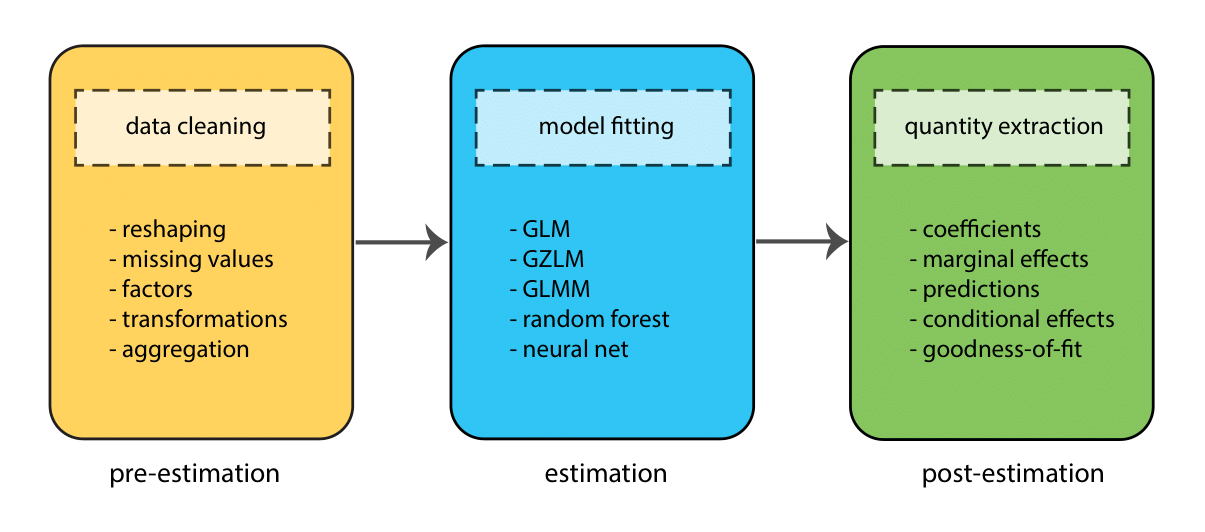
\includegraphics{R/Rmodels/images/R_model_pipeline.png}
\caption{}
\end{figure}

Throughout this workshop we will go through these stages several times
as we fit different types of model.

\section{R modeling ecosystem}\label{r-modeling-ecosystem}

There are literally hundreds of R packages that provide model fitting
functionality. We're going to focus on just two during this workshop ---
\texttt{stats}, from Base R, and \texttt{lme4}. It's a good idea to look
at \href{https://cran.r-project.org/web/views/}{CRAN Task Views} when
trying to find a modeling package for your needs, as they provide an
extensive curated list. But, here's a more digestable table showing some
of the most popular packages for particular types of model.

\begin{longtable}[]{@{}ll@{}}
\toprule
Models & Packages\tabularnewline
\midrule
\endhead
Generalized linear & \texttt{stats}, \texttt{biglm}, \texttt{MASS},
\texttt{robustbase}\tabularnewline
Mixed effects & \texttt{lme4}, \texttt{nlme}, \texttt{glmmTMB},
\texttt{MASS}\tabularnewline
Econometric & \texttt{pglm}, \texttt{VGAM}, \texttt{pscl},
\texttt{survival}\tabularnewline
Bayesian & \texttt{brms}, \texttt{blme}, \texttt{MCMCglmm},
\texttt{rstan}\tabularnewline
Machine learning & \texttt{mlr}, \texttt{caret}, \texttt{h2o},
\texttt{tensorflow}\tabularnewline
\bottomrule
\end{longtable}

\section{Before fitting a model}\label{before-fitting-a-model}

\textbf{GOAL: To learn about the data by creating summaries and
visualizations.}

One important part of the pre-estimation stage of model fitting, is
gaining an understanding of the data we wish to model by creating plots
and summaries. Let's do this now.

\subsection{Load the data}\label{load-the-data}

List the data files we're going to work with:

\begin{Shaded}
\begin{Highlighting}[]
\KeywordTok{list.files}\NormalTok{(}\StringTok{"dataSets"}\NormalTok{)}
\end{Highlighting}
\end{Shaded}

\begin{verbatim}
## [1] "Exam.rds"          "NatHealth2008MI"   "NatHealth2011.rds" "states.rds"
\end{verbatim}

We're going to use the \texttt{states} data first, which originally
appeared in \emph{Statistics with Stata} by Lawrence C. Hamilton.

\begin{Shaded}
\begin{Highlighting}[]
  \CommentTok{# read the states data}
\NormalTok{  states_data <-}\StringTok{ }\KeywordTok{read_rds}\NormalTok{(}\StringTok{"dataSets/states.rds"}\NormalTok{)}

  \CommentTok{# look at the last few rows}
  \KeywordTok{tail}\NormalTok{(states_data)}
\end{Highlighting}
\end{Shaded}

\begin{verbatim}
##            state  region     pop  area density metro waste energy miles toxic green house senate csat vsat msat percent expense income high college
## 46       Vermont N. East  563000  9249   60.87  23.4  0.69    232  10.4  1.81 15.17    85     94  890  424  466      68    6738 34.717 80.8    24.3
## 47      Virginia   South 6187000 39598  156.25  72.5  1.45    306   9.7 12.87 18.72    33     54  890  424  466      60    4836 38.838 75.2    24.5
## 48    Washington    West 4867000 66582   73.10  81.7  1.05    389   9.2  8.51 16.51    52     64  913  433  480      49    5000 36.338 83.8    22.9
## 49 West Virginia   South 1793000 24087   74.44  36.4  0.95    415   8.6 21.30 51.14    48     57  926  441  485      17    4911 24.233 66.0    12.3
##  [ reached 'max' / getOption("max.print") -- omitted 2 rows ]
\end{verbatim}

\begin{longtable}[]{@{}ll@{}}
\toprule
Variable & Description\tabularnewline
\midrule
\endhead
csat & Mean composite SAT score\tabularnewline
expense & Per pupil expenditures\tabularnewline
percent & \% HS graduates taking SAT\tabularnewline
income & Median household income, \$1,000\tabularnewline
region & Geographic region: West, N. East, South, Midwest\tabularnewline
house & House '91 environ. voting, \%\tabularnewline
senate & Senate '91 environ. voting, \%\tabularnewline
energy & Per capita energy consumed, Btu\tabularnewline
metro & Metropolitan area population, \%\tabularnewline
waste & Per capita solid waste, tons\tabularnewline
\bottomrule
\end{longtable}

\subsection{Examine the data}\label{examine-the-data}

Start by examining the data to check for problems.

\begin{Shaded}
\begin{Highlighting}[]
  \CommentTok{# summary of expense and csat columns, all rows}
\NormalTok{  sts_ex_sat <-}\StringTok{ }
\StringTok{      }\NormalTok{states_data }\OperatorTok\StringTok{ }
\StringTok{      }\KeywordTok{select}\NormalTok{(expense, csat)}
  
  \KeywordTok{summary}\NormalTok{(sts_ex_sat)}
\end{Highlighting}
\end{Shaded}

\begin{verbatim}
##     expense          csat     
##  Min.   :2960   Min.   : 832  
##  1st Qu.:4352   1st Qu.: 888  
##  Median :5000   Median : 926  
##  Mean   :5236   Mean   : 944  
##  3rd Qu.:5794   3rd Qu.: 997  
##  Max.   :9259   Max.   :1093
\end{verbatim}

\begin{Shaded}
\begin{Highlighting}[]
  \CommentTok{# correlation between expense and csat}
  \KeywordTok{cor}\NormalTok{(sts_ex_sat, }\DataTypeTok{use =} \StringTok{"pairwise"}\NormalTok{) }
\end{Highlighting}
\end{Shaded}

\begin{verbatim}
##           expense      csat
## expense  1.000000 -0.466298
## csat    -0.466298  1.000000
\end{verbatim}

\subsection{Plot the data}\label{plot-the-data}

Plot the data to look for multivariate outliers, non-linear
relationships etc.

\begin{Shaded}
\begin{Highlighting}[]
  \CommentTok{# scatter plot of expense vs csat}
  \KeywordTok{plot}\NormalTok{(sts_ex_sat)}
\end{Highlighting}
\end{Shaded}

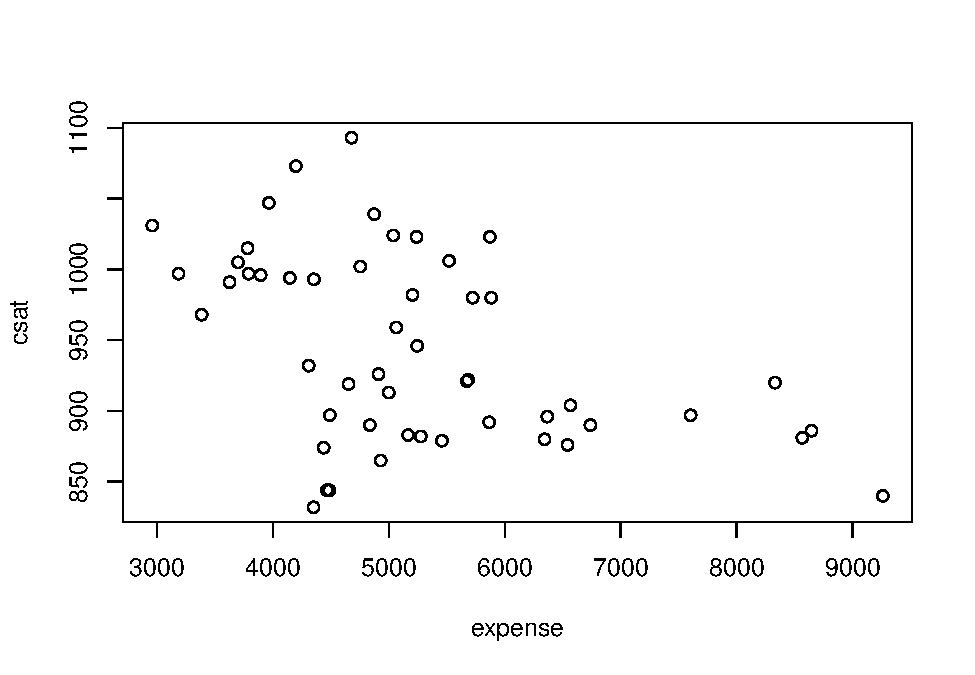
\includegraphics{R/Rmodels/figures/unnamed-chunk-85-1.pdf}

\begin{figure}
\centering
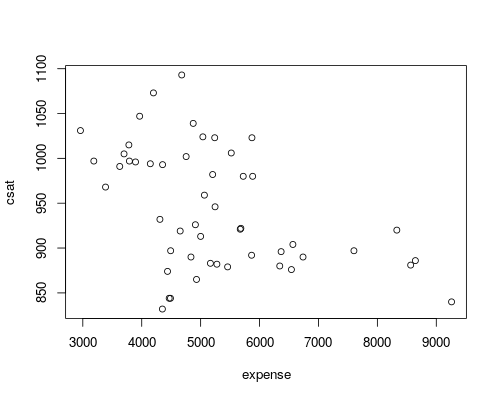
\includegraphics{R/Rmodels/images/statesCorr1.png}
\caption{}
\end{figure}

Obviously, in a real project, you would want to spend more time
investigating the data, but we'll now move on to modeling.

\section{Models with continuous
outcomes}\label{models-with-continuous-outcomes}

\textbf{GOAL: To learn about the R modeling ecosystem by fitting
ordinary least squares (OLS) models.} In particular:

\begin{enumerate}
\def\labelenumi{\arabic{enumi}.}
\tightlist
\item
  Formula representation of a model specification
\item
  Model classes
\item
  Function methods
\item
  Model comparison
\end{enumerate}

Once the data have been inspected and cleaned, we can start estimating
models. The simplest models (but those with the most assumptions) are
those for continuous and unbounded outcomes. Typically, for these
outcomes, we'd use a model estimated using Ordinary Least Lquares (OLS),
which in R can be fit with the \texttt{lm()} (linear model) function.

To fit a model in R, we first have to convert our theoretical model into
a \texttt{formula} --- a symbolic representation of the model in R
syntax:

\begin{Shaded}
\begin{Highlighting}[]
\CommentTok{# formula for model specification}
\NormalTok{outcome }\OperatorTok{~}\StringTok{ }\NormalTok{pred1 }\OperatorTok{+}\StringTok{ }\NormalTok{pred2 }\OperatorTok{+}\StringTok{ }\NormalTok{pred3}

\CommentTok{# }\AlertTok{NOTE}\CommentTok{ the ~ is a tilde}
\end{Highlighting}
\end{Shaded}

For example, the following model predicts SAT scores based on per-pupil
expenditures:

\[
csat_i = \beta_01 + \beta_1expense_i + \epsilon_i
\]

We can use \texttt{lm()} to fit this model:

\begin{Shaded}
\begin{Highlighting}[]
  \CommentTok{# Fit our regression model}
\NormalTok{  sat_mod <-}\StringTok{ }\KeywordTok{lm}\NormalTok{(csat }\OperatorTok{~}\StringTok{ }\DecValTok{1} \OperatorTok{+}\StringTok{ }\NormalTok{expense, }\CommentTok{# regression formula}
                \DataTypeTok{data =}\NormalTok{ states_data) }\CommentTok{# data }
                
  \CommentTok{# Summarize and print the results}
  \KeywordTok{summary}\NormalTok{(sat_mod) }\OperatorTok\StringTok{ }\KeywordTok{coef}\NormalTok{() }\CommentTok{# show regression coefficients table}
\end{Highlighting}
\end{Shaded}

\begin{verbatim}
##                 Estimate  Std. Error  t value    Pr(>|t|)
## (Intercept) 1060.7324439 32.70089674 32.43741 8.87841e-35
## expense       -0.0222756  0.00603711 -3.68978 5.63090e-04
\end{verbatim}

\subsection{\texorpdfstring{Why is the association between expense \&
SAT scores
\emph{negative}?}{Why is the association between expense \& SAT scores negative?}}\label{why-is-the-association-between-expense-sat-scores-negative}

Many people find it surprising that the per-capita expenditure on
students is negatively related to SAT scores. The beauty of multiple
regression is that we can try to pull these apart. What would the
association between expense and SAT scores be if there were no
difference among the states in the percentage of students taking the
SAT?

\begin{Shaded}
\begin{Highlighting}[]
  \KeywordTok{lm}\NormalTok{(csat }\OperatorTok{~}\StringTok{ }\DecValTok{1} \OperatorTok{+}\StringTok{ }\NormalTok{expense }\OperatorTok{+}\StringTok{ }\NormalTok{percent, }\DataTypeTok{data =}\NormalTok{ states_data) }\OperatorTok\StringTok{ }
\StringTok{  }\KeywordTok{summary}\NormalTok{() }
\end{Highlighting}
\end{Shaded}

\begin{verbatim}
## 
## Call:
## lm(formula = csat ~ 1 + expense + percent, data = states_data)
## 
## Residuals:
##    Min     1Q Median     3Q    Max 
## -62.92 -24.32   1.74  15.50  75.62 
## 
## Coefficients:
##             Estimate Std. Error t value           Pr(>|t|)
## (Intercept) 989.8074    18.3958   53.81            < 2e-16
## expense       0.0086     0.0042    2.05              0.046
## percent      -2.5377     0.2249  -11.28 0.0000000000000042
## 
## Residual standard error: 31.6 on 48 degrees of freedom
## Multiple R-squared:  0.786,  Adjusted R-squared:  0.777 
## F-statistic:   88 on 2 and 48 DF,  p-value: <2e-16
\end{verbatim}

\subsection{\texorpdfstring{The \texttt{lm} class \&
methods}{The lm class \& methods}}\label{the-lm-class-methods}

Okay, we fitted our model. Now what? Typically, the main goal in the
\textbf{post-estimation stage} of analysis is to extract
\textbf{quantities of interest} from our fitted model. These quantities
could be things like:

\begin{enumerate}
\def\labelenumi{\arabic{enumi}.}
\tightlist
\item
  Testing whether one group is different on average from another group
\item
  Generating average response values from the model for interesting
  combinations of predictor values
\item
  Calculating interval estimates for particular coefficients
\end{enumerate}

But before we can do any of that, we need to know more about
\textbf{what a fitted model actually is,} \textbf{what information it
contains, and how we can extract from it information that we want to
report}.

Let's start by examining the model object:

\begin{Shaded}
\begin{Highlighting}[]
  \KeywordTok{class}\NormalTok{(sat_mod)}
\end{Highlighting}
\end{Shaded}

\begin{verbatim}
## [1] "lm"
\end{verbatim}

\begin{Shaded}
\begin{Highlighting}[]
  \KeywordTok{str}\NormalTok{(sat_mod)}
\end{Highlighting}
\end{Shaded}

\begin{verbatim}
## List of 12
##  $ coefficients : Named num [1:2] 1060.7324 -0.0223
##   ..- attr(*, "names")= chr [1:2] "(Intercept)" "expense"
##  $ residuals    : Named num [1:51] 11.1 44.8 -32.7 26.7 -63.7 ...
##   ..- attr(*, "names")= chr [1:51] "1" "2" "3" "4" ...
##  $ effects      : Named num [1:51] -6742.2 220.7 -31.7 29.7 -63.2 ...
##   ..- attr(*, "names")= chr [1:51] "(Intercept)" "expense" "" "" ...
##  $ rank         : int 2
##  $ fitted.values: Named num [1:51] 980 875 965 978 961 ...
##   ..- attr(*, "names")= chr [1:51] "1" "2" "3" "4" ...
##  $ assign       : int [1:2] 0 1
##  $ qr           :List of 5
##   ..$ qr   : num [1:51, 1:2] -7.14 0.14 0.14 0.14 0.14 ...
##   .. ..- attr(*, "dimnames")=List of 2
##   .. .. ..$ : chr [1:51] "1" "2" "3" "4" ...
##   .. .. ..$ : chr [1:2] "(Intercept)" "expense"
##   .. ..- attr(*, "assign")= int [1:2] 0 1
##   ..$ qraux: num [1:2] 1.14 1.33
##   ..$ pivot: int [1:2] 1 2
##   ..$ tol  : num 0.0000001
##   ..$ rank : int 2
##   ..- attr(*, "class")= chr "qr"
##  $ df.residual  : int 49
##  $ xlevels      : Named list()
##  $ call         : language lm(formula = csat ~ 1 + expense, data = states_data)
##  $ terms        :Classes 'terms', 'formula'  language csat ~ 1 + expense
##   .. ..- attr(*, "variables")= language list(csat, expense)
##   .. ..- attr(*, "factors")= int [1:2, 1] 0 1
##   .. .. ..- attr(*, "dimnames")=List of 2
##   .. .. .. ..$ : chr [1:2] "csat" "expense"
##   .. .. .. ..$ : chr "expense"
##   .. ..- attr(*, "term.labels")= chr "expense"
##   .. ..- attr(*, "order")= int 1
##   .. ..- attr(*, "intercept")= int 1
##   .. ..- attr(*, "response")= int 1
##   .. ..- attr(*, ".Environment")=<environment: R_GlobalEnv> 
##   .. ..- attr(*, "predvars")= language list(csat, expense)
##   .. ..- attr(*, "dataClasses")= Named chr [1:2] "numeric" "numeric"
##   .. .. ..- attr(*, "names")= chr [1:2] "csat" "expense"
##  $ model        :'data.frame':   51 obs. of  2 variables:
##   ..$ csat   : int [1:51] 991 920 932 1005 897 959 897 892 840 882 ...
##   ..$ expense: int [1:51] 3627 8330 4309 3700 4491 5064 7602 5865 9259 5276 ...
##   ..- attr(*, "terms")=Classes 'terms', 'formula'  language csat ~ 1 + expense
##   .. .. ..- attr(*, "variables")= language list(csat, expense)
##   .. .. ..- attr(*, "factors")= int [1:2, 1] 0 1
##   .. .. .. ..- attr(*, "dimnames")=List of 2
##   .. .. .. .. ..$ : chr [1:2] "csat" "expense"
##   .. .. .. .. ..$ : chr "expense"
##   .. .. ..- attr(*, "term.labels")= chr "expense"
##   .. .. ..- attr(*, "order")= int 1
##   .. .. ..- attr(*, "intercept")= int 1
##   .. .. ..- attr(*, "response")= int 1
##   .. .. ..- attr(*, ".Environment")=<environment: R_GlobalEnv> 
##   .. .. ..- attr(*, "predvars")= language list(csat, expense)
##   .. .. ..- attr(*, "dataClasses")= Named chr [1:2] "numeric" "numeric"
##   .. .. .. ..- attr(*, "names")= chr [1:2] "csat" "expense"
##  - attr(*, "class")= chr "lm"
\end{verbatim}

\begin{Shaded}
\begin{Highlighting}[]
  \KeywordTok{names}\NormalTok{(sat_mod)}
\end{Highlighting}
\end{Shaded}

\begin{verbatim}
##  [1] "coefficients"  "residuals"     "effects"       "rank"          "fitted.values" "assign"        "qr"            "df.residual"   "xlevels"       "call"          "terms"         "model"
\end{verbatim}

\begin{Shaded}
\begin{Highlighting}[]
  \KeywordTok{methods}\NormalTok{(}\DataTypeTok{class =} \KeywordTok{class}\NormalTok{(sat_mod))}
\end{Highlighting}
\end{Shaded}

\begin{verbatim}
##  [1] add1           addterm        alias          anova          boxcox         case.names     coerce         confint        cooks.distance deviance       dfbeta         dfbetas        drop1          dropterm      
## [15] dummy.coef     Effect         effects        emm_basis      extractAIC     family         formula        fortify        hatvalues      influence      initialize     kappa          labels         logLik        
## [29] logtrans       model.frame    model.matrix   nobs           plot           predict        print          proj           qqnorm         qr             recover_data   residuals      rstandard      rstudent      
## [43] show           simulate       slotsFromS3    summary        variable.names vcov          
## see '?methods' for accessing help and source code
\end{verbatim}

We can use \texttt{function\ methods} to get more information about the
fit:

\begin{Shaded}
\begin{Highlighting}[]
  \KeywordTok{summary}\NormalTok{(sat_mod)}
\end{Highlighting}
\end{Shaded}

\begin{verbatim}
## 
## Call:
## lm(formula = csat ~ 1 + expense, data = states_data)
## 
## Residuals:
##     Min      1Q  Median      3Q     Max 
## -131.81  -38.08    5.61   37.85  136.50 
## 
## Coefficients:
##               Estimate Std. Error t value Pr(>|t|)
## (Intercept) 1060.73244   32.70090   32.44  < 2e-16
## expense       -0.02228    0.00604   -3.69  0.00056
## 
## Residual standard error: 59.8 on 49 degrees of freedom
## Multiple R-squared:  0.217,  Adjusted R-squared:  0.201 
## F-statistic: 13.6 on 1 and 49 DF,  p-value: 0.000563
\end{verbatim}

\begin{Shaded}
\begin{Highlighting}[]
  \KeywordTok{summary}\NormalTok{(sat_mod) }\OperatorTok\StringTok{ }\KeywordTok{coef}\NormalTok{()}
\end{Highlighting}
\end{Shaded}

\begin{verbatim}
##                 Estimate  Std. Error  t value    Pr(>|t|)
## (Intercept) 1060.7324439 32.70089674 32.43741 8.87841e-35
## expense       -0.0222756  0.00603711 -3.68978 5.63090e-04
\end{verbatim}

\begin{Shaded}
\begin{Highlighting}[]
  \KeywordTok{methods}\NormalTok{(}\StringTok{"summary"}\NormalTok{)}
\end{Highlighting}
\end{Shaded}

\begin{verbatim}
##   [1] summary,ANY-method             summary,DBIObject-method       summary,diagonalMatrix-method  summary,sparseMatrix-method    summary.aareg*                 summary.allFit*               
##   [7] summary.aov                    summary.aovlist*               summary.aspell*                summary.cch*                   summary.check_packages_in_dir* summary.connection            
##  [13] summary.corAR1*                summary.corARMA*               summary.corCAR1*               summary.corCompSymm*           summary.corExp*                summary.corGaus*              
##  [19] summary.corIdent*              summary.corLin*                summary.corNatural*            summary.corRatio*              summary.corSpher*              summary.corStruct*            
##  [25] summary.corSymm*               summary.coxph*                 summary.coxph.penal*           summary.data.frame             summary.Date                   summary.DBIrepdesign*         
##  [31] summary.DBIsvydesign*          summary.default                summary.Duration*              summary.ecdf*                  summary.eff*                   summary.efflatent*            
##  [37] summary.efflist*               summary.effpoly*               summary.emm_list*              summary.emmGrid*               summary.factor                 summary.ggplot*               
##  [43] summary.glht*                  summary.glht_list*             summary.glm                    summary.gls*                   summary.hcl_palettes*          summary.infl*                 
##  [49] summary.Interval*              summary.lm                     summary.lme*                   summary.lmList*                summary.lmList4*               summary.loess*                
##  [55] summary.loglm*                 summary.manova                 summary.matrix                 summary.mcmc*                  summary.mcmc.list*             summary.merMod*               
##  [61] summary.MIresult*              summary.mlm*                   summary.mlm.efflist*           summary.modelStruct*           summary.multinom*              summary.negbin*               
##  [67] summary.nls*                   summary.nlsList*               summary.nnet*                  summary.ODBCrepdesign*         summary.ODBCsvydesign*         summary.packageStatus*        
##  [73] summary.pdBlocked*             summary.pdCompSymm*            summary.pdDiag*                summary.pdIdent*               summary.pdLogChol*             summary.pdMat*                
##  [79] summary.pdNatural*             summary.pdSymm*                summary.Period*                summary.polr*                  summary.POSIXct                summary.POSIXlt               
##  [85] summary.ppr*                   summary.pps*                   summary.prcomp*                summary.prcomplist*            summary.predictorefflist*      summary.princomp*             
##  [91] summary.proc_time              summary.pyears*                summary.ratetable*             summary.reStruct*              summary.rlang_error*           summary.rlang_trace*          
##  [97] summary.rlm*                   summary.shingle*               summary.srcfile                summary.srcref                
##  [ reached getOption("max.print") -- omitted 36 entries ]
## see '?methods' for accessing help and source code
\end{verbatim}

\begin{Shaded}
\begin{Highlighting}[]
  \KeywordTok{confint}\NormalTok{(sat_mod)}
\end{Highlighting}
\end{Shaded}

\begin{verbatim}
##                   2.5 %       97.5 %
## (Intercept) 995.0175316 1126.4473563
## expense      -0.0344077   -0.0101436
\end{verbatim}

How does R know which method to call for a given object? R uses
\texttt{generic\ functions}, which provide access to \texttt{methods}.
Method dispatch takes place based on the \texttt{class} of the first
argument to the generic function. For example, for the generic function
\texttt{summary()} and an object of class \texttt{lm}, the method
dispatched will be \texttt{summary.lm()}. Function methods always take
the form \texttt{generic.method()}:

\begin{figure}
\centering
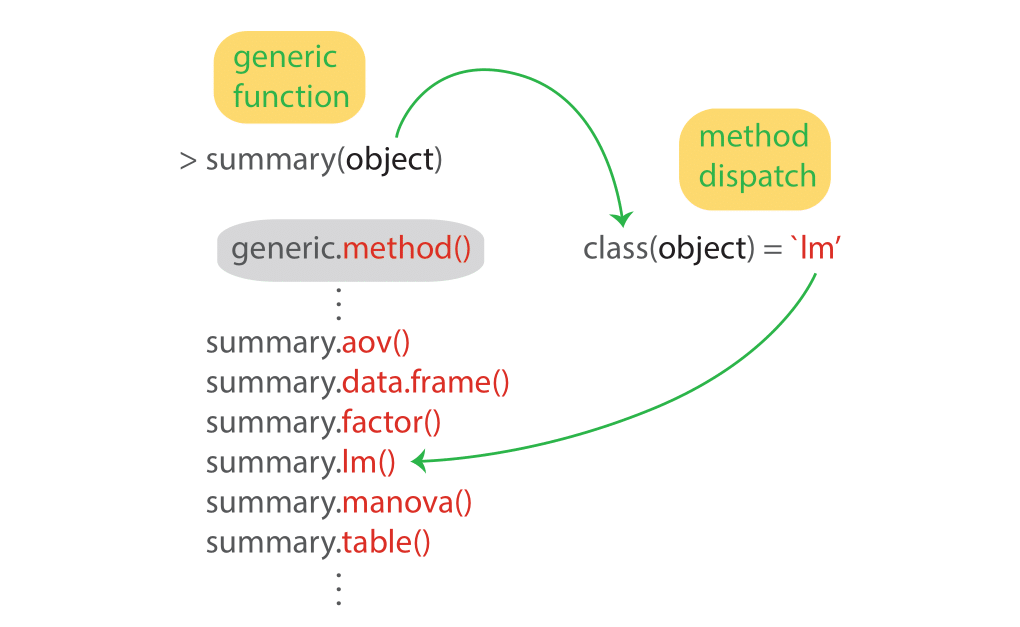
\includegraphics{R/Rmodels/images/methods.png}
\caption{}
\end{figure}

It's always worth examining what function methods are available for the
class of model you're fitting. Here's a summary table of some of the
most often used methods. These are post-estimation tools you will want
in your toolbox:

\begin{longtable}[]{@{}lll@{}}
\toprule
\begin{minipage}[b]{0.16\columnwidth}\raggedright\strut
Function\strut
\end{minipage} & \begin{minipage}[b]{0.17\columnwidth}\raggedright\strut
Package\strut
\end{minipage} & \begin{minipage}[b]{0.58\columnwidth}\raggedright\strut
Output\strut
\end{minipage}\tabularnewline
\midrule
\endhead
\begin{minipage}[t]{0.16\columnwidth}\raggedright\strut
\texttt{summary()}\strut
\end{minipage} & \begin{minipage}[t]{0.17\columnwidth}\raggedright\strut
\texttt{stats} base R\strut
\end{minipage} & \begin{minipage}[t]{0.58\columnwidth}\raggedright\strut
standard errors, test statistics, p-values, GOF stats\strut
\end{minipage}\tabularnewline
\begin{minipage}[t]{0.16\columnwidth}\raggedright\strut
\texttt{confint()}\strut
\end{minipage} & \begin{minipage}[t]{0.17\columnwidth}\raggedright\strut
\texttt{stats} base R\strut
\end{minipage} & \begin{minipage}[t]{0.58\columnwidth}\raggedright\strut
confidence intervals\strut
\end{minipage}\tabularnewline
\begin{minipage}[t]{0.16\columnwidth}\raggedright\strut
\texttt{anova()}\strut
\end{minipage} & \begin{minipage}[t]{0.17\columnwidth}\raggedright\strut
\texttt{stats} base R\strut
\end{minipage} & \begin{minipage}[t]{0.58\columnwidth}\raggedright\strut
anova table (one model), model comparison (\textgreater{} one
model)\strut
\end{minipage}\tabularnewline
\begin{minipage}[t]{0.16\columnwidth}\raggedright\strut
\texttt{coef()}\strut
\end{minipage} & \begin{minipage}[t]{0.17\columnwidth}\raggedright\strut
\texttt{stats} base R\strut
\end{minipage} & \begin{minipage}[t]{0.58\columnwidth}\raggedright\strut
point estimates\strut
\end{minipage}\tabularnewline
\begin{minipage}[t]{0.16\columnwidth}\raggedright\strut
\texttt{drop1()}\strut
\end{minipage} & \begin{minipage}[t]{0.17\columnwidth}\raggedright\strut
\texttt{stats} base R\strut
\end{minipage} & \begin{minipage}[t]{0.58\columnwidth}\raggedright\strut
model comparison\strut
\end{minipage}\tabularnewline
\begin{minipage}[t]{0.16\columnwidth}\raggedright\strut
\texttt{predict()}\strut
\end{minipage} & \begin{minipage}[t]{0.17\columnwidth}\raggedright\strut
\texttt{stats} base R\strut
\end{minipage} & \begin{minipage}[t]{0.58\columnwidth}\raggedright\strut
predicted response values\strut
\end{minipage}\tabularnewline
\begin{minipage}[t]{0.16\columnwidth}\raggedright\strut
\texttt{fitted()}\strut
\end{minipage} & \begin{minipage}[t]{0.17\columnwidth}\raggedright\strut
\texttt{stats} base R\strut
\end{minipage} & \begin{minipage}[t]{0.58\columnwidth}\raggedright\strut
predicted response values (for observed data)\strut
\end{minipage}\tabularnewline
\begin{minipage}[t]{0.16\columnwidth}\raggedright\strut
\texttt{residuals()}\strut
\end{minipage} & \begin{minipage}[t]{0.17\columnwidth}\raggedright\strut
\texttt{stats} base R\strut
\end{minipage} & \begin{minipage}[t]{0.58\columnwidth}\raggedright\strut
residuals\strut
\end{minipage}\tabularnewline
\begin{minipage}[t]{0.16\columnwidth}\raggedright\strut
\texttt{fixef()}\strut
\end{minipage} & \begin{minipage}[t]{0.17\columnwidth}\raggedright\strut
\texttt{lme4}\strut
\end{minipage} & \begin{minipage}[t]{0.58\columnwidth}\raggedright\strut
fixed effect point estimates (mixed models only)\strut
\end{minipage}\tabularnewline
\begin{minipage}[t]{0.16\columnwidth}\raggedright\strut
\texttt{ranef()}\strut
\end{minipage} & \begin{minipage}[t]{0.17\columnwidth}\raggedright\strut
\texttt{lme4}\strut
\end{minipage} & \begin{minipage}[t]{0.58\columnwidth}\raggedright\strut
random effect point estimates (mixed models only)\strut
\end{minipage}\tabularnewline
\begin{minipage}[t]{0.16\columnwidth}\raggedright\strut
\texttt{coef()}\strut
\end{minipage} & \begin{minipage}[t]{0.17\columnwidth}\raggedright\strut
\texttt{lme4}\strut
\end{minipage} & \begin{minipage}[t]{0.58\columnwidth}\raggedright\strut
empirical Bayes estimates (mixed models only)\strut
\end{minipage}\tabularnewline
\begin{minipage}[t]{0.16\columnwidth}\raggedright\strut
\texttt{allEffects()}\strut
\end{minipage} & \begin{minipage}[t]{0.17\columnwidth}\raggedright\strut
\texttt{effects}\strut
\end{minipage} & \begin{minipage}[t]{0.58\columnwidth}\raggedright\strut
predicted marginal means\strut
\end{minipage}\tabularnewline
\begin{minipage}[t]{0.16\columnwidth}\raggedright\strut
\texttt{emmeans()}\strut
\end{minipage} & \begin{minipage}[t]{0.17\columnwidth}\raggedright\strut
\texttt{emmeans}\strut
\end{minipage} & \begin{minipage}[t]{0.58\columnwidth}\raggedright\strut
predicted marginal means \& marginal effects\strut
\end{minipage}\tabularnewline
\begin{minipage}[t]{0.16\columnwidth}\raggedright\strut
\texttt{margins()}\strut
\end{minipage} & \begin{minipage}[t]{0.17\columnwidth}\raggedright\strut
\texttt{margins}\strut
\end{minipage} & \begin{minipage}[t]{0.58\columnwidth}\raggedright\strut
predicted marginal means \& marginal effects\strut
\end{minipage}\tabularnewline
\bottomrule
\end{longtable}

\subsection{OLS regression
assumptions}\label{ols-regression-assumptions}

OLS regression relies on several assumptions, including:

\begin{enumerate}
\def\labelenumi{\arabic{enumi}.}
\tightlist
\item
  The model includes all relevant variables (i.e., no omitted variable
  bias).
\item
  The model is linear in the parameters (i.e., the coefficients and
  error term).
\item
  The error term has an expected value of zero.
\item
  All right-hand-side variables are uncorrelated with the error term.
\item
  No right-hand-side variables are a perfect linear function of other
  RHS variables.
\item
  Observations of the error term are uncorrelated with each other.
\item
  The error term has constant variance (i.e., homoscedasticity).
\item
  (Optional - only needed for inference). The error term is normally
  distributed.
\end{enumerate}

Investigate assumptions \#7 and \#8 visually by plotting your model:

\begin{Shaded}
\begin{Highlighting}[]
  \KeywordTok{par}\NormalTok{(}\DataTypeTok{mfrow =} \KeywordTok{c}\NormalTok{(}\DecValTok{2}\NormalTok{, }\DecValTok{2}\NormalTok{)) }\CommentTok{# splits the plotting window into 4 panels}
  \KeywordTok{plot}\NormalTok{(sat_mod)}
\end{Highlighting}
\end{Shaded}

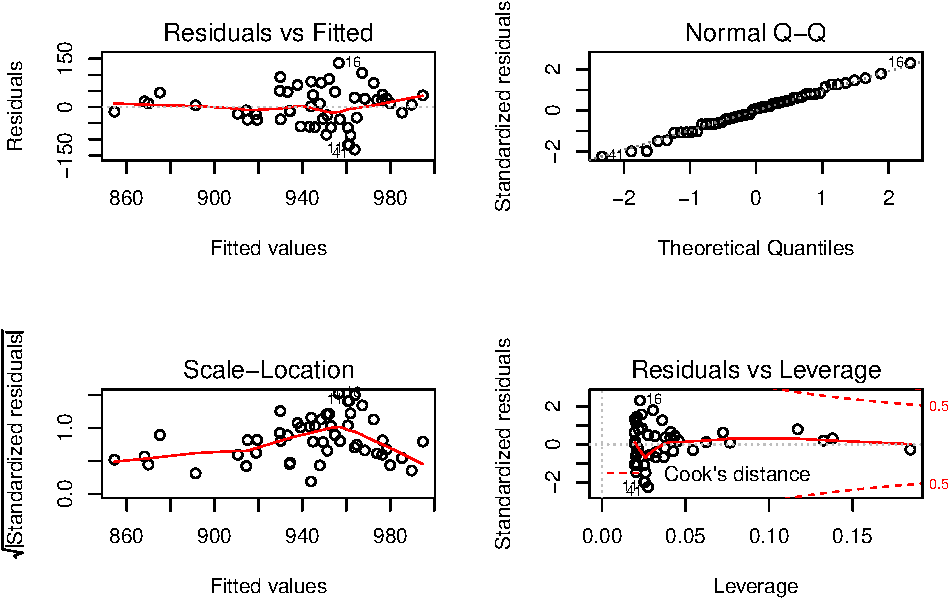
\includegraphics{R/Rmodels/figures/unnamed-chunk-91-1.pdf}

\subsection{Comparing models}\label{comparing-models}

Do congressional voting patterns predict SAT scores over and above
expense? Fit two models and compare them:

\begin{Shaded}
\begin{Highlighting}[]
  \CommentTok{# fit another model, adding house and senate as predictors}
\NormalTok{  sat_voting_mod <-}\StringTok{ }\KeywordTok{lm}\NormalTok{(csat }\OperatorTok{~}\StringTok{ }\DecValTok{1} \OperatorTok{+}\StringTok{ }\NormalTok{expense }\OperatorTok{+}\StringTok{ }\NormalTok{house }\OperatorTok{+}\StringTok{ }\NormalTok{senate,}
                        \DataTypeTok{data =} \KeywordTok{na.omit}\NormalTok{(states_data))}

  \KeywordTok{summary}\NormalTok{(sat_voting_mod) }\OperatorTok\StringTok{ }\KeywordTok{coef}\NormalTok{()}
\end{Highlighting}
\end{Shaded}

\begin{verbatim}
##                 Estimate  Std. Error   t value    Pr(>|t|)
## (Intercept) 1082.9343804 38.63381274 28.030741 1.06779e-29
## expense       -0.0187083  0.00969149 -1.930385 6.00200e-02
## house         -1.4424375  0.60047838 -2.402147 2.05867e-02
## senate         0.4981786  0.51356136  0.970047 3.37326e-01
\end{verbatim}

Why are we using \texttt{na.omit()}? Let's see what \texttt{na.omit()}
does.

\begin{Shaded}
\begin{Highlighting}[]
\CommentTok{# fake data}
\NormalTok{dat <-}\StringTok{ }\KeywordTok{data.frame}\NormalTok{(}
  \DataTypeTok{x =} \DecValTok{1}\OperatorTok{:}\DecValTok{5}\NormalTok{,}
  \DataTypeTok{y =} \KeywordTok{c}\NormalTok{(}\DecValTok{3}\NormalTok{, }\DecValTok{2}\NormalTok{, }\DecValTok{1}\NormalTok{, }\OtherTok{NA}\NormalTok{, }\DecValTok{5}\NormalTok{),}
  \DataTypeTok{z =} \KeywordTok{c}\NormalTok{(}\DecValTok{6}\NormalTok{, }\OtherTok{NA}\NormalTok{, }\DecValTok{2}\NormalTok{, }\DecValTok{7}\NormalTok{, }\DecValTok{3}\NormalTok{))}
\NormalTok{dat}
\end{Highlighting}
\end{Shaded}

\begin{verbatim}
##   x  y  z
## 1 1  3  6
## 2 2  2 NA
## 3 3  1  2
## 4 4 NA  7
## 5 5  5  3
\end{verbatim}

\begin{Shaded}
\begin{Highlighting}[]
\KeywordTok{na.omit}\NormalTok{(dat) }\CommentTok{# listwise deletion of observations}
\end{Highlighting}
\end{Shaded}

\begin{verbatim}
##   x y z
## 1 1 3 6
## 3 3 1 2
## 5 5 5 3
\end{verbatim}

\begin{Shaded}
\begin{Highlighting}[]
\CommentTok{# also see}
\CommentTok{# ?complete.cases}
\NormalTok{dat[}\KeywordTok{with}\NormalTok{(dat, }\KeywordTok{complete.cases}\NormalTok{(x, y, z)), ]}
\end{Highlighting}
\end{Shaded}

\begin{verbatim}
##   x y z
## 1 1 3 6
## 3 3 1 2
## 5 5 5 3
\end{verbatim}

To compare models, we must fit them to the same data. This is why we
need \texttt{na.omit()}. Now let's update our first model using
\texttt{na.omit()}:

\begin{Shaded}
\begin{Highlighting}[]
\NormalTok{  sat_mod <-}\StringTok{ }\KeywordTok{update}\NormalTok{(sat_mod, }\DataTypeTok{data =} \KeywordTok{na.omit}\NormalTok{(states_data))}

  \CommentTok{# compare using an F-test with the anova() function}
  \KeywordTok{anova}\NormalTok{(sat_mod, sat_voting_mod)}
\end{Highlighting}
\end{Shaded}

\begin{verbatim}
## Analysis of Variance Table
## 
## Model 1: csat ~ 1 + expense
## Model 2: csat ~ 1 + expense + house + senate
##   Res.Df    RSS Df Sum of Sq     F Pr(>F)
## 1     46 169050                          
## 2     44 149284  2     19766 2.913 0.0649
\end{verbatim}

\subsection{Exercise 0}\label{exercise-0-1}

\textbf{Ordinary least squares regression}

Use the \emph{states.rds} data set. Fit a model predicting energy
consumed per capita (energy) from the percentage of residents living in
metropolitan areas (\texttt{metro}). Be sure to

\begin{enumerate}
\def\labelenumi{\arabic{enumi}.}
\tightlist
\item
  Examine/plot the data before fitting the model
\end{enumerate}

\begin{Shaded}
\begin{Highlighting}[]
\NormalTok{## }
\end{Highlighting}
\end{Shaded}

\begin{enumerate}
\def\labelenumi{\arabic{enumi}.}
\setcounter{enumi}{1}
\tightlist
\item
  Print and interpret the model \texttt{summary()}
\end{enumerate}

\begin{Shaded}
\begin{Highlighting}[]
\NormalTok{## }
\end{Highlighting}
\end{Shaded}

\begin{enumerate}
\def\labelenumi{\arabic{enumi}.}
\setcounter{enumi}{2}
\tightlist
\item
  \texttt{plot()} the model to look for deviations from modeling
  assumptions
\end{enumerate}

\begin{Shaded}
\begin{Highlighting}[]
\NormalTok{## }
\end{Highlighting}
\end{Shaded}

\begin{enumerate}
\def\labelenumi{\arabic{enumi}.}
\setcounter{enumi}{3}
\tightlist
\item
  Select one or more additional predictors to add to your model and
  repeat steps 1-3. Is this model significantly better than the model
  with \texttt{metro} as the only predictor?
\end{enumerate}

\begin{Shaded}
\begin{Highlighting}[]
\NormalTok{## }
\end{Highlighting}
\end{Shaded}

\section{Interactions \& factors}\label{interactions-factors}

\textbf{GOAL: To learn how to specify interaction effects and fit models
with categorical predictors.} In particular:

\begin{enumerate}
\def\labelenumi{\arabic{enumi}.}
\tightlist
\item
  Formula syntax for interaction effects
\item
  Factor levels and labels
\item
  Contrasts and pairwise comparisons
\end{enumerate}

\subsection{Modeling interactions}\label{modeling-interactions}

Interactions allow us assess the extent to which the association between
one predictor and the outcome depends on a second predictor. For
example: Does the association between expense and SAT scores depend on
the median income in the state?

\begin{Shaded}
\begin{Highlighting}[]
  \CommentTok{# Add the interaction to the model}
\NormalTok{  sat_expense_by_percent <-}\StringTok{ }\KeywordTok{lm}\NormalTok{(csat }\OperatorTok{~}\StringTok{ }\DecValTok{1} \OperatorTok{+}\StringTok{ }\NormalTok{expense }\OperatorTok{+}\StringTok{ }\NormalTok{income }\OperatorTok{+}\StringTok{ }\NormalTok{expense }\OperatorTok{:}\StringTok{ }\NormalTok{income, }\DataTypeTok{data =}\NormalTok{ states_data)}

  \CommentTok{# same as above, but shorter syntax}
\NormalTok{  sat_expense_by_percent <-}\StringTok{ }\KeywordTok{lm}\NormalTok{(csat }\OperatorTok{~}\StringTok{ }\DecValTok{1} \OperatorTok{+}\StringTok{ }\NormalTok{expense }\OperatorTok{*}\StringTok{ }\NormalTok{income, }\DataTypeTok{data =}\NormalTok{ states_data) }

  \CommentTok{# Show the regression coefficients table}
  \KeywordTok{summary}\NormalTok{(sat_expense_by_percent) }\OperatorTok\StringTok{ }\KeywordTok{coef}\NormalTok{() }
\end{Highlighting}
\end{Shaded}

\begin{verbatim}
##                     Estimate    Std. Error  t value          Pr(>|t|)
## (Intercept)    1380.36423333 172.086252477  8.02135 0.000000000236707
## expense          -0.06384067   0.032700873 -1.95226 0.056878369245142
## income          -10.49785114   4.991463374 -2.10316 0.040832525070882
## expense:income    0.00138465   0.000863553  1.60343 0.115539488252897
\end{verbatim}

\subsection{Regression with categorical
predictors}\label{regression-with-categorical-predictors}

Let's try to predict SAT scores from region, a categorical variable.
Note that you must make sure R does not think your categorical variable
is numeric.

\begin{Shaded}
\begin{Highlighting}[]
  \CommentTok{# make sure R knows region is categorical}
  \KeywordTok{str}\NormalTok{(states_data}\OperatorTok{$}\NormalTok{region)}
\end{Highlighting}
\end{Shaded}

\begin{verbatim}
##  Factor w/ 4 levels "West","N. East",..: 3 1 1 3 1 1 2 3 NA 3 ...
\end{verbatim}

\begin{Shaded}
\begin{Highlighting}[]
\NormalTok{  states_data}\OperatorTok{$}\NormalTok{region <-}\StringTok{ }\KeywordTok{factor}\NormalTok{(states_data}\OperatorTok{$}\NormalTok{region)}

  \CommentTok{# arguments to the factor() function}
  \CommentTok{# factor(x, levels, labels)}

  \KeywordTok{levels}\NormalTok{(states_data}\OperatorTok{$}\NormalTok{region)}
\end{Highlighting}
\end{Shaded}

\begin{verbatim}
## [1] "West"    "N. East" "South"   "Midwest"
\end{verbatim}

\begin{Shaded}
\begin{Highlighting}[]
  \CommentTok{# Add region to the model}
\NormalTok{  sat_region <-}\StringTok{ }\KeywordTok{lm}\NormalTok{(csat }\OperatorTok{~}\StringTok{ }\DecValTok{1} \OperatorTok{+}\StringTok{ }\NormalTok{region, }\DataTypeTok{data =}\NormalTok{ states_data) }

  \CommentTok{# Show the results}
  \KeywordTok{summary}\NormalTok{(sat_region) }\OperatorTok\StringTok{ }\KeywordTok{coef}\NormalTok{() }\CommentTok{# show the regression coefficients table}
\end{Highlighting}
\end{Shaded}

\begin{verbatim}
##               Estimate Std. Error   t value    Pr(>|t|)
## (Intercept)   946.3077    14.7958 63.957781 1.35258e-46
## regionN. East -56.7521    23.1328 -2.453314 1.80038e-02
## regionSouth   -16.3077    19.9195 -0.818681 4.17190e-01
## regionMidwest  63.7756    21.3559  2.986321 4.51415e-03
\end{verbatim}

\begin{Shaded}
\begin{Highlighting}[]
  \KeywordTok{anova}\NormalTok{(sat_region) }\CommentTok{# show ANOVA table}
\end{Highlighting}
\end{Shaded}

\begin{verbatim}
## Analysis of Variance Table
## 
## Response: csat
##           Df Sum Sq Mean Sq F value    Pr(>F)
## region     3  82049   27350    9.61 0.0000486
## Residuals 46 130912    2846
\end{verbatim}

So, make sure to tell R which variables are categorical by converting
them to factors!

\subsection{Setting factor reference groups \&
contrasts}\label{setting-factor-reference-groups-contrasts}

\textbf{Contrasts} is the umbrella term used to describe the process of
testing linear combinations of parameters from regression models. All
statistical sofware use contrasts, but each sofware has different
defaults and their own way of overriding these.

The default contrasts in R are ``treatment'' contrasts (aka ``dummy
coding''), where each level within a factor is identified within a
matrix of binary \texttt{0} / \texttt{1} variables, with the first level
chosen as the reference category. They're called ``treatment''
contrasts, because of the typical use case where there is one control
group (the reference group) and one or more treatment groups that are to
be compared to the controls. It is easy to change the default contrasts
to something other than treatment contrasts, though this is rarely
needed. More often, we may want to change the reference group in
treatment contrasts or get all sets of pairwise contrasts between factor
levels.

\begin{Shaded}
\begin{Highlighting}[]
  \CommentTok{# change the reference group}
\NormalTok{  states_data}\OperatorTok{$}\NormalTok{region <-}\StringTok{ }\KeywordTok{relevel}\NormalTok{(states_data}\OperatorTok{$}\NormalTok{region, }\DataTypeTok{ref =} \StringTok{"Midwest"}\NormalTok{)}
\NormalTok{  m1 <-}\StringTok{ }\KeywordTok{lm}\NormalTok{(csat }\OperatorTok{~}\StringTok{ }\DecValTok{1} \OperatorTok{+}\StringTok{ }\NormalTok{region, }\DataTypeTok{data =}\NormalTok{ states_data)}
  \KeywordTok{summary}\NormalTok{(m1) }\OperatorTok\StringTok{ }\KeywordTok{coef}\NormalTok{()}
\end{Highlighting}
\end{Shaded}

\begin{verbatim}
##                Estimate Std. Error  t value    Pr(>|t|)
## (Intercept)   1010.0833    15.4000 65.58993 4.29631e-47
## regionWest     -63.7756    21.3559 -2.98632 4.51415e-03
## regionN. East -120.5278    23.5239 -5.12364 5.79840e-06
## regionSouth    -80.0833    20.3723 -3.93100 2.82601e-04
\end{verbatim}

\begin{Shaded}
\begin{Highlighting}[]
  \CommentTok{# get all pairwise contrasts between means}
\NormalTok{  means <-}\StringTok{ }\KeywordTok{emmeans}\NormalTok{(m1, }\DataTypeTok{specs =} \OperatorTok{~}\StringTok{ }\NormalTok{region)}
\NormalTok{  means}
\end{Highlighting}
\end{Shaded}

\begin{verbatim}
##  region  emmean   SE df lower.CL upper.CL
##  Midwest   1010 15.4 46      979     1041
##  West       946 14.8 46      917      976
##  N. East    890 17.8 46      854      925
##  South      930 13.3 46      903      957
## 
## Confidence level used: 0.95
\end{verbatim}

\begin{Shaded}
\begin{Highlighting}[]
  \KeywordTok{contrast}\NormalTok{(means, }\DataTypeTok{method =} \StringTok{"pairwise"}\NormalTok{)}
\end{Highlighting}
\end{Shaded}

\begin{verbatim}
##  contrast          estimate   SE df t.ratio p.value
##  Midwest - West        63.8 21.4 46  2.986  0.0226 
##  Midwest - N. East    120.5 23.5 46  5.124  <.0001 
##  Midwest - South       80.1 20.4 46  3.931  0.0016 
##  West - N. East        56.8 23.1 46  2.453  0.0812 
##  West - South          16.3 19.9 46  0.819  0.8453 
##  N. East - South      -40.4 22.2 46 -1.820  0.2774 
## 
## P value adjustment: tukey method for comparing a family of 4 estimates
\end{verbatim}

\subsection{Exercise 1}\label{exercise-1-1}

\textbf{Interactions \& factors}

Use the \texttt{states} data set.

\begin{enumerate}
\def\labelenumi{\arabic{enumi}.}
\tightlist
\item
  Add on to the regression equation that you created in Exercise 1 by
  generating an interaction term and testing the interaction.
\end{enumerate}

\begin{Shaded}
\begin{Highlighting}[]
\NormalTok{## }
\end{Highlighting}
\end{Shaded}

\begin{enumerate}
\def\labelenumi{\arabic{enumi}.}
\setcounter{enumi}{1}
\tightlist
\item
  Try adding region to the model. Are there significant differences
  across the four regions?
\end{enumerate}

\begin{Shaded}
\begin{Highlighting}[]
\NormalTok{## }
\end{Highlighting}
\end{Shaded}

\section{Models with binary outcomes}\label{models-with-binary-outcomes}

\textbf{GOAL: To learn how to use the \texttt{glm()} function to model
binary outcomes.} In particular:

\begin{enumerate}
\def\labelenumi{\arabic{enumi}.}
\tightlist
\item
  The \texttt{family} and \texttt{link} components of the \texttt{glm()}
  function call
\item
  Transforming model coefficients into odds ratios
\item
  Transforming model coefficients into predicted marginal means
\end{enumerate}

\subsection{Logistic regression}\label{logistic-regression}

This far we have used the \texttt{lm()} function to fit our regression
models. \texttt{lm()} is great, but limited --- in particular it only
fits models for continuous dependent variables. For categorical
dependent variables we can use the \texttt{glm()} function.

For these models we will use a different dataset, drawn from the
National Health Interview Survey. From the
\href{http://www.cdc.gov/nchs/nhis.htm}{CDC website}:

\begin{quote}
The National Health Interview Survey (NHIS) has monitored the health of
the nation since 1957. NHIS data on a broad range of health topics are
collected through personal household interviews. For over 50 years, the
U.S. Census Bureau has been the data collection agent for the National
Health Interview Survey. Survey results have been instrumental in
providing data to track health status, health care access, and progress
toward achieving national health objectives.
\end{quote}

Load the National Health Interview Survey data:

\begin{Shaded}
\begin{Highlighting}[]
\NormalTok{  NH11 <-}\StringTok{ }\KeywordTok{read_rds}\NormalTok{(}\StringTok{"dataSets/NatHealth2011.rds"}\NormalTok{)}
\end{Highlighting}
\end{Shaded}

\subsection{Logistic regression
example}\label{logistic-regression-example}

Motivation for a logistic regression model --- with a binary response:

\begin{enumerate}
\def\labelenumi{\arabic{enumi}.}
\tightlist
\item
  Errors will not be normally distributed
\item
  Variance will not be homoskedastic
\item
  Predictions should be constrained to be on the interval {[}0, 1{]}
\end{enumerate}

\begin{figure}
\centering
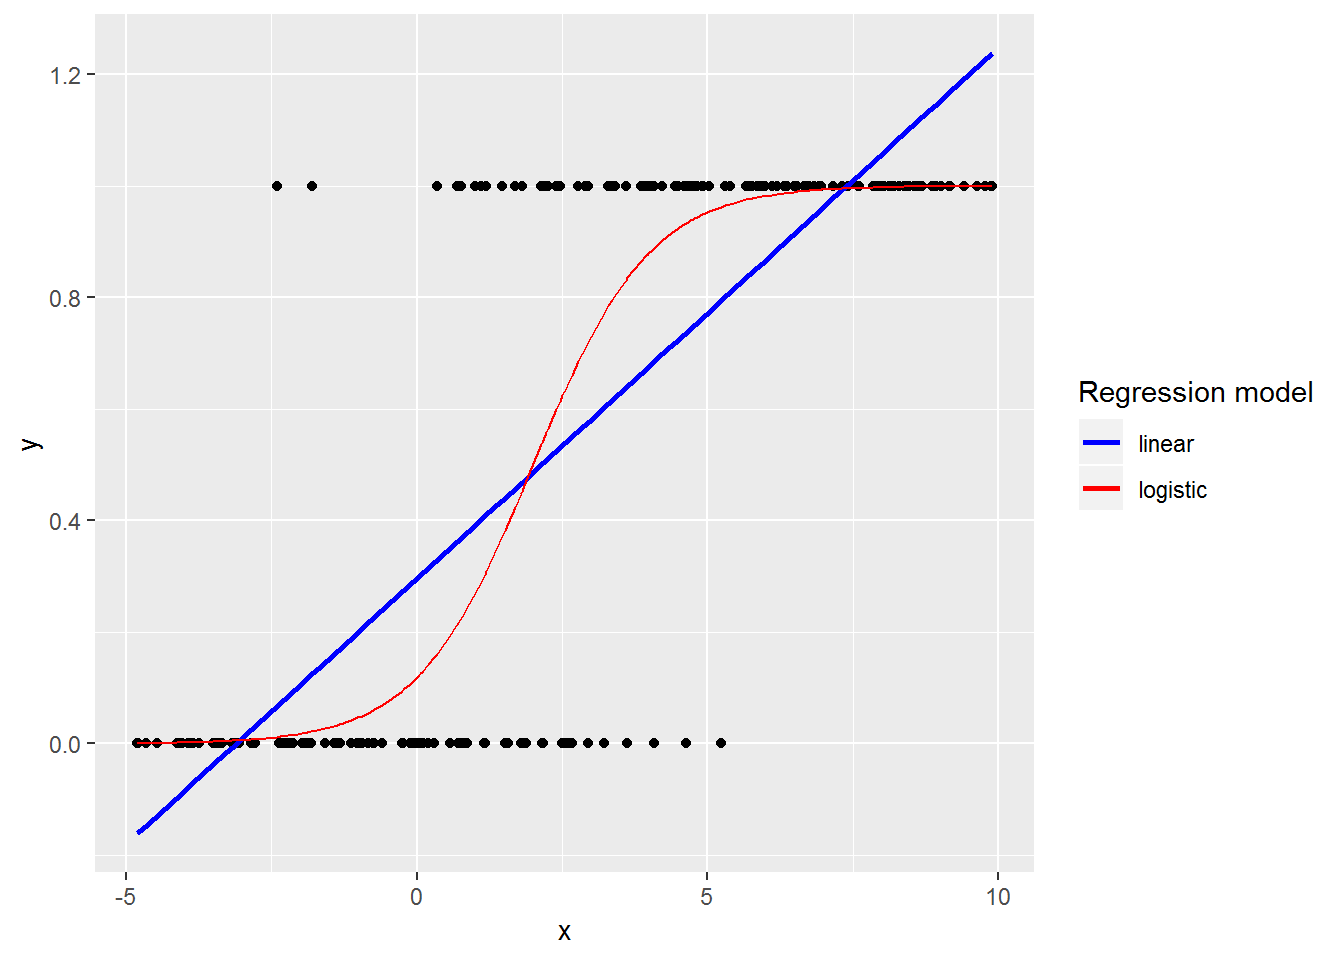
\includegraphics{R/Rmodels/images/logistic.png}
\caption{}
\end{figure}

Anatomy of a generalized linear model:

\begin{Shaded}
\begin{Highlighting}[]
  \CommentTok{# OLS model using lm()}
  \KeywordTok{lm}\NormalTok{(outcome }\OperatorTok{~}\StringTok{ }\DecValTok{1} \OperatorTok{+}\StringTok{ }\NormalTok{pred1 }\OperatorTok{+}\StringTok{ }\NormalTok{pred2, }
     \DataTypeTok{data =}\NormalTok{ mydata)}

  \CommentTok{# OLS model using glm()}
  \KeywordTok{glm}\NormalTok{(outcome }\OperatorTok{~}\StringTok{ }\DecValTok{1} \OperatorTok{+}\StringTok{ }\NormalTok{pred1 }\OperatorTok{+}\StringTok{ }\NormalTok{pred2, }
      \DataTypeTok{data =}\NormalTok{ mydata, }
      \DataTypeTok{family =} \KeywordTok{gaussian}\NormalTok{(}\DataTypeTok{link =} \StringTok{"identity"}\NormalTok{))}
 
  \CommentTok{# logistic model using glm()}
  \KeywordTok{glm}\NormalTok{(outcome }\OperatorTok{~}\StringTok{ }\DecValTok{1} \OperatorTok{+}\StringTok{ }\NormalTok{pred1 }\OperatorTok{+}\StringTok{ }\NormalTok{pred2, }
      \DataTypeTok{data =}\NormalTok{ mydata, }
      \DataTypeTok{family =} \KeywordTok{binomial}\NormalTok{(}\DataTypeTok{link =} \StringTok{"logit"}\NormalTok{))}
\end{Highlighting}
\end{Shaded}

The \texttt{family} argument sets the error distribution for the model,
while the \texttt{link} function argument relates the predictors to the
expected value of the outcome.

Let's predict the probability of being diagnosed with hypertension based
on \texttt{age}, \texttt{sex}, \texttt{sleep}, and \texttt{bmi}. Here's
the model:

\[
logit(hypev_i) = \beta_01 + \beta_1agep_i + \beta_2sex_i + \beta_3sleep_i + \beta_4bmi_i + \epsilon_i 
\]

where \(logit(\cdot)\) is the link function, which is equivalent to the
log odds of \texttt{hypev}:

\[
logit(hypev_i) = ln \frac{p(hypev_i = 1)}{p(hypev_i = 0)}
\]

And here's how we fit this in R. First, let's clean up the hypertension
outcome by making it binary:

\begin{Shaded}
\begin{Highlighting}[]
  \KeywordTok{str}\NormalTok{(NH11}\OperatorTok{$}\NormalTok{hypev) }\CommentTok{# check stucture of hypev}
\end{Highlighting}
\end{Shaded}

\begin{verbatim}
##  Factor w/ 5 levels "1 Yes","2 No",..: 2 2 1 2 2 1 2 2 1 2 ...
\end{verbatim}

\begin{Shaded}
\begin{Highlighting}[]
  \KeywordTok{levels}\NormalTok{(NH11}\OperatorTok{$}\NormalTok{hypev) }\CommentTok{# check levels of hypev}
\end{Highlighting}
\end{Shaded}

\begin{verbatim}
## [1] "1 Yes"             "2 No"              "7 Refused"         "8 Not ascertained" "9 Don't know"
\end{verbatim}

\begin{Shaded}
\begin{Highlighting}[]
  \CommentTok{# collapse all missing values to NA}
\NormalTok{  NH11}\OperatorTok{$}\NormalTok{hypev <-}\StringTok{ }\KeywordTok{factor}\NormalTok{(NH11}\OperatorTok{$}\NormalTok{hypev, }\DataTypeTok{levels=}\KeywordTok{c}\NormalTok{(}\StringTok{"2 No"}\NormalTok{, }\StringTok{"1 Yes"}\NormalTok{))}
\end{Highlighting}
\end{Shaded}

Now let's use \texttt{glm()} to estimate the model:

\begin{Shaded}
\begin{Highlighting}[]
  \CommentTok{# run our regression model}
\NormalTok{  hyp_out <-}\StringTok{ }\KeywordTok{glm}\NormalTok{(hypev }\OperatorTok{~}\StringTok{ }\DecValTok{1} \OperatorTok{+}\StringTok{ }\NormalTok{age_p }\OperatorTok{+}\StringTok{ }\NormalTok{sex }\OperatorTok{+}\StringTok{ }\NormalTok{sleep }\OperatorTok{+}\StringTok{ }\NormalTok{bmi,}
                 \DataTypeTok{data =}\NormalTok{ NH11, }
                 \DataTypeTok{family =} \KeywordTok{binomial}\NormalTok{(}\DataTypeTok{link =} \StringTok{"logit"}\NormalTok{))}

  \KeywordTok{summary}\NormalTok{(hyp_out) }\OperatorTok\StringTok{ }\KeywordTok{coef}\NormalTok{()}
\end{Highlighting}
\end{Shaded}

\begin{verbatim}
##                Estimate  Std. Error   z value    Pr(>|z|)
## (Intercept) -4.26946603 0.056494729 -75.57282 0.00000e+00
## age_p        0.06069930 0.000822721  73.77874 0.00000e+00
## sex2 Female -0.14402509 0.026797660  -5.37454 7.67785e-08
## sleep       -0.00703578 0.001639720  -4.29084 1.77998e-05
## bmi          0.01857170 0.000951083  19.52691 6.48517e-85
\end{verbatim}

\subsection{Odds ratios}\label{odds-ratios}

Generalized linear models use link functions to relate the average value
of the response to the predictors, so raw coefficients are difficult to
interpret. For example, the \texttt{age} coefficient of .06 in the
previous model tells us that for every one unit increase in
\texttt{age}, the log odds of hypertension diagnosis increases by 0.06.
Since most of us are not used to thinking in log odds this is not too
helpful!

One solution is to transform the coefficients to make them easier to
interpret. Here we transform them into odds ratios by exponentiating:

\begin{Shaded}
\begin{Highlighting}[]
  \CommentTok{# point estimates}
  \KeywordTok{coef}\NormalTok{(hyp_out) }\OperatorTok\StringTok{ }\KeywordTok{exp}\NormalTok{()}
\end{Highlighting}
\end{Shaded}

\begin{verbatim}
## (Intercept)       age_p sex2 Female       sleep         bmi 
##   0.0139893   1.0625794   0.8658660   0.9929889   1.0187452
\end{verbatim}

\begin{Shaded}
\begin{Highlighting}[]
  \CommentTok{# confidence intervals}
  \KeywordTok{confint}\NormalTok{(hyp_out) }\OperatorTok\StringTok{ }\KeywordTok{exp}\NormalTok{()}
\end{Highlighting}
\end{Shaded}

\begin{verbatim}
##                 2.5 %    97.5 %
## (Intercept) 0.0125168 0.0156197
## age_p       1.0608738 1.0643008
## sex2 Female 0.8215520 0.9125501
## sleep       0.9897876 0.9961747
## bmi         1.0168514 1.0206501
\end{verbatim}

\subsection{Predicted marginal means}\label{predicted-marginal-means}

Instead of reporting odds ratios, we may want to calculate predicted
marginal means (sometimes called ``least squares means''). These are
average values of the outcome at particular levels of the predictors.
For ease of interpretation, we want these marginal means to be on the
response scale (i.e., the probability scale). We can use the
\texttt{effects} package to compute these quantities of interest for us
(by default, the numerical output will be on the response scale).

\begin{Shaded}
\begin{Highlighting}[]
\NormalTok{  eff <-}\StringTok{ }\KeywordTok{allEffects}\NormalTok{(hyp_out)}
  \KeywordTok{plot}\NormalTok{(eff, }\DataTypeTok{type =} \StringTok{"response"}\NormalTok{) }\CommentTok{# "response" refers to the probability scale}
\end{Highlighting}
\end{Shaded}

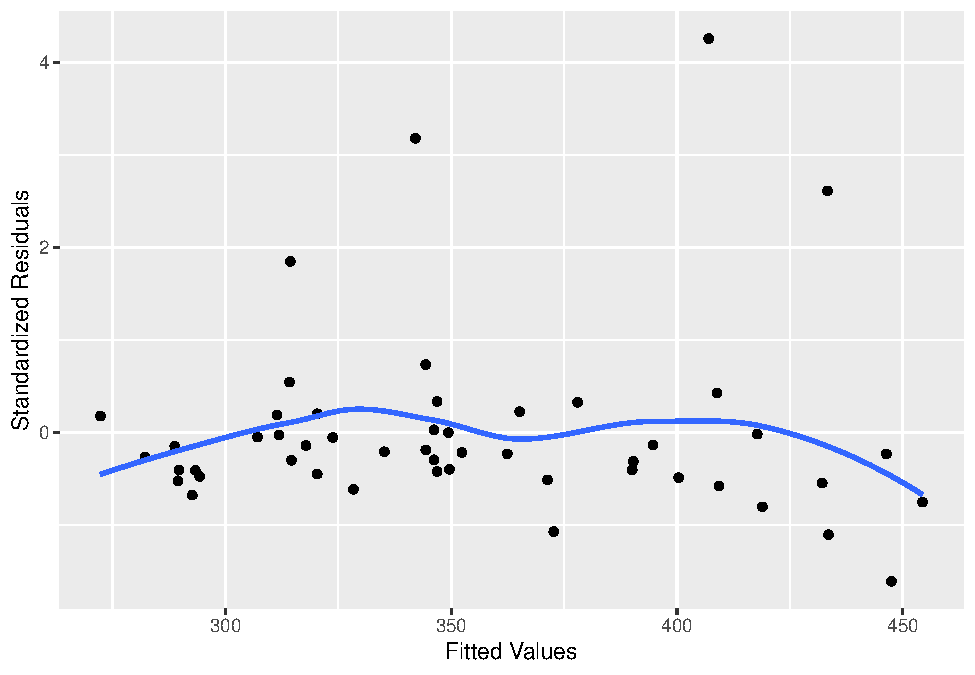
\includegraphics{R/Rmodels/figures/unnamed-chunk-110-1.pdf}

\begin{Shaded}
\begin{Highlighting}[]
  \CommentTok{# generate a sequence at which to get predictions of the outcome}
  \KeywordTok{seq}\NormalTok{(}\DecValTok{20}\NormalTok{, }\DecValTok{80}\NormalTok{, }\DataTypeTok{by =} \DecValTok{5}\NormalTok{)}
\end{Highlighting}
\end{Shaded}

\begin{verbatim}
##  [1] 20 25 30 35 40 45 50 55 60 65 70 75 80
\end{verbatim}

\begin{Shaded}
\begin{Highlighting}[]
  \CommentTok{# override defaults}
\NormalTok{  eff <-}\StringTok{ }\KeywordTok{allEffects}\NormalTok{(hyp_out, }\DataTypeTok{xlevels =} \KeywordTok{list}\NormalTok{(}\DataTypeTok{age_p =} \KeywordTok{seq}\NormalTok{(}\DecValTok{20}\NormalTok{, }\DecValTok{80}\NormalTok{, }\DataTypeTok{by =} \DecValTok{5}\NormalTok{)))}
\NormalTok{  eff_df <-}\StringTok{ }\KeywordTok{as.data.frame}\NormalTok{(eff) }\CommentTok{# confidence intervals}
\NormalTok{  eff_df}
\end{Highlighting}
\end{Shaded}

\begin{verbatim}
## $age_p
##    age_p       fit         se     lower     upper
## 1     20 0.0669038 0.00191570 0.0632455 0.0707578
## 2     25 0.0885269 0.00218162 0.0843432 0.0928971
## 3     30 0.1162677 0.00241881 0.1116102 0.1210931
## 4     35 0.1512588 0.00260324 0.1462269 0.1564320
## 5     40 0.1944632 0.00272243 0.1891828 0.1998547
## 6     45 0.2464253 0.00279626 0.2409858 0.2519468
## 7     50 0.3069807 0.00289586 0.3013344 0.3126855
## 8     55 0.3750116 0.00312411 0.3689087 0.3811544
## 9     60 0.4483648 0.00353179 0.4414530 0.4552965
## 10    65 0.5240356 0.00405245 0.5160876 0.5319716
## 11    70 0.5986188 0.00454553 0.5896780 0.6074944
## 12    75 0.6688990 0.00488073 0.6592642 0.6783943
## 13    80 0.7323751 0.00498654 0.7224891 0.7420346
## 
## $sex
##        sex      fit         se    lower    upper
## 1   1 Male 0.299419 0.00418871 0.291274 0.307692
## 2 2 Female 0.270104 0.00371503 0.262885 0.277447
## 
## $sleep
##   sleep      fit         se    lower    upper
## 1     3 0.289994 0.00327643 0.283615 0.296458
## 2    30 0.252489 0.00742700 0.238212 0.267322
## 3    50 0.226866 0.01244618 0.203401 0.252181
## 4    80 0.191984 0.01854946 0.158220 0.230977
## 5   100 0.171095 0.02158429 0.132829 0.217620
## 
## $bmi
##   bmi      fit         se    lower    upper
## 1  10 0.214408 0.00412159 0.206441 0.222597
## 2  30 0.283509 0.00284941 0.277958 0.289127
## 3  60 0.408549 0.00745016 0.394031 0.423227
## 4  80 0.500366 0.01213914 0.476591 0.524140
## 5 100 0.592159 0.01618007 0.560105 0.623448
\end{verbatim}

\begin{figure}
\centering
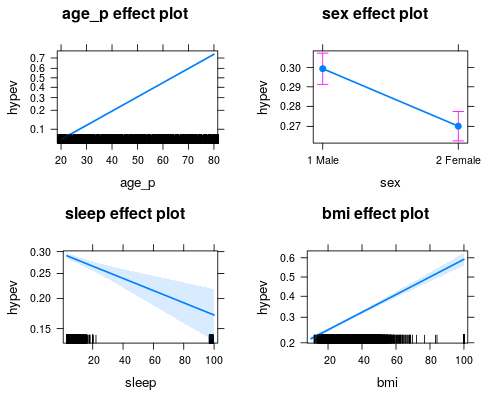
\includegraphics{R/Rmodels/images/effects1.png}
\caption{}
\end{figure}

\subsection{Exercise 2}\label{exercise-2}

\textbf{Logistic regression}

Use the \texttt{NH11} data set that we loaded earlier.

\begin{enumerate}
\def\labelenumi{\arabic{enumi}.}
\tightlist
\item
  Use \texttt{glm()} to conduct a logistic regression to predict ever
  worked (\texttt{everwrk}) using age (\texttt{age\_p}) and marital
  status (\texttt{r\_maritl}). Make sure you only keep the following two
  levels for \texttt{everwrk} (\texttt{1\ Yes} and \texttt{2\ No}).
  Hint: use the \texttt{factor()} function. Also, make sure to drop any
  \texttt{r\_maritl} levels that do not contain observations. Hint: see
  \texttt{?droplevels}.
\end{enumerate}

\begin{Shaded}
\begin{Highlighting}[]
\NormalTok{## }
\end{Highlighting}
\end{Shaded}

\begin{enumerate}
\def\labelenumi{\arabic{enumi}.}
\setcounter{enumi}{1}
\tightlist
\item
  Predict the probability of working for each level of marital status.
  Hint: use \texttt{allEffects()}
\end{enumerate}

\begin{Shaded}
\begin{Highlighting}[]
\NormalTok{## }
\end{Highlighting}
\end{Shaded}

Note that the data are not perfectly clean and ready to be modeled. You
will need to clean up at least some of the variables before fitting the
model.

\section{Multilevel modeling}\label{multilevel-modeling}

\textbf{GOAL: To learn about how to use the \texttt{lmer()} function to
model clustered data.} In particular:

\begin{enumerate}
\def\labelenumi{\arabic{enumi}.}
\tightlist
\item
  The formula syntax for incorporating random effects into a model
\item
  Calculating the intraclass correlation (ICC)
\item
  Model comparison for fixed and random effects
\end{enumerate}

\subsection{Multilevel modeling
overview}\label{multilevel-modeling-overview}

\begin{itemize}
\tightlist
\item
  Multi-level (AKA hierarchical) models are a type of
  \textbf{mixed-effects} model
\item
  They are used to model data that are clustered (i.e., non-independent)
\item
  Mixed-effecs models include two types of predictors:
  \textbf{fixed-effects} and \textbf{random effects}
\item
  \textbf{Fixed-effects} -- observed levels are of direct interest
  (.e.g, sex, political party\ldots{})
\item
  \textbf{Random-effects} -- observed levels not of direct interest:
  goal is to make inferences to a population represented by observed
  levels
\item
  In R, the \texttt{lme4} package is the most popular for mixed effects
  models
\item
  Use the \texttt{lmer()} function for liner mixed models,
  \texttt{glmer()} for generalized linear mixed models
\end{itemize}

\subsection{The Exam data}\label{the-exam-data}

The Exam data set contans exam scores of 4,059 students from 65 schools
in Inner London. The variable names are as follows:

\begin{longtable}[]{@{}ll@{}}
\toprule
Variable & Description\tabularnewline
\midrule
\endhead
school & School ID - a factor.\tabularnewline
normexam & Normalized exam score.\tabularnewline
standLRT & Standardised LR test score.\tabularnewline
student & Student id (within school) - a factor\tabularnewline
\bottomrule
\end{longtable}

\begin{Shaded}
\begin{Highlighting}[]
\NormalTok{  Exam <-}\StringTok{ }\KeywordTok{read_rds}\NormalTok{(}\StringTok{"dataSets/Exam.rds"}\NormalTok{)}
\end{Highlighting}
\end{Shaded}

\subsection{The null model \& ICC}\label{the-null-model-icc}

As a preliminary step it is often useful to partition the variance in
the dependent variable into the various levels. This can be accomplished
by running a null model (i.e., a model with a random effects grouping
structure, but no fixed-effects predictors).

\begin{Shaded}
\begin{Highlighting}[]
  \CommentTok{# anatomy of lmer() function}
  \KeywordTok{lmer}\NormalTok{(outcome }\OperatorTok{~}\StringTok{ }\DecValTok{1} \OperatorTok{+}\StringTok{ }\NormalTok{pred1 }\OperatorTok{+}\StringTok{ }\NormalTok{pred2 }\OperatorTok{+}\StringTok{ }\NormalTok{(}\DecValTok{1} \OperatorTok{|}\StringTok{ }\NormalTok{grouping_variable), }
       \DataTypeTok{data =}\NormalTok{ mydata, }
       \DataTypeTok{REML =} \OtherTok{FALSE}\NormalTok{)}
\end{Highlighting}
\end{Shaded}

\begin{Shaded}
\begin{Highlighting}[]
  \CommentTok{# null model, grouping by school but not fixed effects.}
\NormalTok{  Norm1 <-}\KeywordTok{lmer}\NormalTok{(normexam }\OperatorTok{~}\StringTok{ }\DecValTok{1} \OperatorTok{+}\StringTok{ }\NormalTok{(}\DecValTok{1} \OperatorTok{|}\StringTok{ }\NormalTok{school), }
              \DataTypeTok{data =} \KeywordTok{na.omit}\NormalTok{(Exam), }\DataTypeTok{REML =} \OtherTok{FALSE}\NormalTok{)}
  \KeywordTok{summary}\NormalTok{(Norm1)}
\end{Highlighting}
\end{Shaded}

\begin{verbatim}
## Linear mixed model fit by maximum likelihood  ['lmerMod']
## Formula: normexam ~ 1 + (1 | school)
##    Data: na.omit(Exam)
## 
##      AIC      BIC   logLik deviance df.resid 
##   9964.9   9983.5  -4979.4   9958.9     3659 
## 
## Scaled residuals: 
##    Min     1Q Median     3Q    Max 
## -3.875 -0.646  0.005  0.690  3.684 
## 
## Random effects:
##  Groups   Name        Variance Std.Dev.
##  school   (Intercept) 0.161    0.401   
##  Residual             0.852    0.923   
## Number of obs: 3662, groups:  school, 65
## 
## Fixed effects:
##             Estimate Std. Error t value
## (Intercept)  -0.0130     0.0527   -0.25
\end{verbatim}

The is .161/(.161 + .852) = .159 = 16\% of the variance is at the school
level.

There is no consensus on how to calculate p-values for MLMs; hence why
they are omitted from the \texttt{lme4} output. But, if you really need
p-values, the \texttt{lmerTest} package will calculate p-values for you
(using the Satterthwaite approximation).

\subsection{Adding fixed-effects
predictors}\label{adding-fixed-effects-predictors}

Here's a model that predicts exam scores from student's standardized
tests scores:

\[
normexam_{ij} = \mu + \beta_1standLRT_{ij} + U_{0j} + \epsilon_{ij}
\]

where \(U_{0j}\) is the random intercept for \texttt{school}. Let's
implement this in R using \texttt{lmer()}:

\begin{Shaded}
\begin{Highlighting}[]
\NormalTok{  Norm2 <-}\KeywordTok{lmer}\NormalTok{(normexam }\OperatorTok{~}\StringTok{ }\DecValTok{1} \OperatorTok{+}\StringTok{ }\NormalTok{standLRT }\OperatorTok{+}\StringTok{ }\NormalTok{(}\DecValTok{1} \OperatorTok{|}\StringTok{ }\NormalTok{school),}
               \DataTypeTok{data =} \KeywordTok{na.omit}\NormalTok{(Exam), }\DataTypeTok{REML =} \OtherTok{FALSE}\NormalTok{) }
  \KeywordTok{summary}\NormalTok{(Norm2) }
\end{Highlighting}
\end{Shaded}

\begin{verbatim}
## Linear mixed model fit by maximum likelihood  ['lmerMod']
## Formula: normexam ~ 1 + standLRT + (1 | school)
##    Data: na.omit(Exam)
## 
##      AIC      BIC   logLik deviance df.resid 
##   8480.1   8505.0  -4236.1   8472.1     3658 
## 
## Scaled residuals: 
##    Min     1Q Median     3Q    Max 
## -3.672 -0.630  0.024  0.677  3.335 
## 
## Random effects:
##  Groups   Name        Variance Std.Dev.
##  school   (Intercept) 0.092    0.303   
##  Residual             0.569    0.754   
## Number of obs: 3662, groups:  school, 65
## 
## Fixed effects:
##              Estimate Std. Error t value
## (Intercept) 0.0000191  0.0402173     0.0
## standLRT    0.5669801  0.0132364    42.8
## 
## Correlation of Fixed Effects:
##          (Intr)
## standLRT 0.007
\end{verbatim}

\subsection{Multiple degree of freedom
comparisons}\label{multiple-degree-of-freedom-comparisons}

As with \texttt{lm()} and \texttt{glm()} models, you can compare the two
\texttt{lmer()} models using a likelihood ratio test with the
\texttt{anova()} function.

\begin{Shaded}
\begin{Highlighting}[]
  \KeywordTok{anova}\NormalTok{(Norm1, Norm2)}
\end{Highlighting}
\end{Shaded}

\begin{verbatim}
## Data: na.omit(Exam)
## Models:
## Norm1: normexam ~ 1 + (1 | school)
## Norm2: normexam ~ 1 + standLRT + (1 | school)
##       Df  AIC  BIC logLik deviance Chisq Chi Df Pr(>Chisq)
## Norm1  3 9965 9984  -4979     9959                        
## Norm2  4 8480 8505  -4236     8472  1487      1     <2e-16
\end{verbatim}

\subsection{Random slopes}\label{random-slopes}

Add a random effect of students' standardized test scores as well. Now
in addition to estimating the distribution of intercepts across schools,
we also estimate the distribution of the slope of exam on standardized
test.

\begin{Shaded}
\begin{Highlighting}[]
\NormalTok{  Norm3 <-}\StringTok{ }\KeywordTok{lmer}\NormalTok{(normexam }\OperatorTok{~}\StringTok{ }\DecValTok{1} \OperatorTok{+}\StringTok{ }\NormalTok{standLRT }\OperatorTok{+}\StringTok{ }\NormalTok{(}\DecValTok{1} \OperatorTok{+}\StringTok{ }\NormalTok{standLRT }\OperatorTok{|}\StringTok{ }\NormalTok{school), }
                \DataTypeTok{data =} \KeywordTok{na.omit}\NormalTok{(Exam), }\DataTypeTok{REML =} \OtherTok{FALSE}\NormalTok{) }
  \KeywordTok{summary}\NormalTok{(Norm3) }
\end{Highlighting}
\end{Shaded}

\begin{verbatim}
## Linear mixed model fit by maximum likelihood  ['lmerMod']
## Formula: normexam ~ 1 + standLRT + (1 + standLRT | school)
##    Data: na.omit(Exam)
## 
##      AIC      BIC   logLik deviance df.resid 
##   8444.1   8481.4  -4216.1   8432.1     3656 
## 
## Scaled residuals: 
##    Min     1Q Median     3Q    Max 
## -3.789 -0.623  0.024  0.674  3.437 
## 
## Random effects:
##  Groups   Name        Variance Std.Dev. Corr
##  school   (Intercept) 0.0893   0.299        
##           standLRT    0.0159   0.126    0.50
##  Residual             0.5559   0.746        
## Number of obs: 3662, groups:  school, 65
## 
## Fixed effects:
##             Estimate Std. Error t value
## (Intercept)  -0.0124     0.0398   -0.31
## standLRT      0.5611     0.0210   26.71
## 
## Correlation of Fixed Effects:
##          (Intr)
## standLRT 0.361
\end{verbatim}

\subsection{Test the significance of the random
slope}\label{test-the-significance-of-the-random-slope}

To test the significance of a random slope just compare models with and
without the random slope term using a likelihood ratio test:

\begin{Shaded}
\begin{Highlighting}[]
  \KeywordTok{anova}\NormalTok{(Norm2, Norm3) }
\end{Highlighting}
\end{Shaded}

\begin{verbatim}
## Data: na.omit(Exam)
## Models:
## Norm2: normexam ~ 1 + standLRT + (1 | school)
## Norm3: normexam ~ 1 + standLRT + (1 + standLRT | school)
##       Df  AIC  BIC logLik deviance Chisq Chi Df    Pr(>Chisq)
## Norm2  4 8480 8505  -4236     8472                           
## Norm3  6 8444 8481  -4216     8432 40.01      2 0.00000000205
\end{verbatim}

\subsection{Exercise 3}\label{exercise-3-1}

\textbf{Multilevel modeling}

Use the \texttt{bh1996} dataset:

\begin{Shaded}
\begin{Highlighting}[]
\NormalTok{## install.packages("multilevel")}
\KeywordTok{data}\NormalTok{(bh1996, }\DataTypeTok{package=}\StringTok{"multilevel"}\NormalTok{)}
\end{Highlighting}
\end{Shaded}

From the data documentation:

\begin{quote}
Variables are Leadership Climate (\texttt{LEAD}), Well-Being
(\texttt{WBEING}), and Work Hours (\texttt{HRS}). The group identifier
is named \texttt{GRP}.
\end{quote}

\begin{enumerate}
\def\labelenumi{\arabic{enumi}.}
\tightlist
\item
  Create a null model predicting wellbeing (\texttt{WBEING})
\end{enumerate}

\begin{Shaded}
\begin{Highlighting}[]
\NormalTok{## }
\end{Highlighting}
\end{Shaded}

\begin{enumerate}
\def\labelenumi{\arabic{enumi}.}
\setcounter{enumi}{1}
\tightlist
\item
  Calculate the ICC for your null model
\end{enumerate}

\begin{Shaded}
\begin{Highlighting}[]
\NormalTok{## }
\end{Highlighting}
\end{Shaded}

\begin{enumerate}
\def\labelenumi{\arabic{enumi}.}
\setcounter{enumi}{2}
\tightlist
\item
  Run a second multi-level model that adds two individual-level
  predictors, average number of hours worked (\texttt{HRS}) and
  leadership skills (\texttt{LEAD}) to the model and interpret your
  output.
\end{enumerate}

\begin{Shaded}
\begin{Highlighting}[]
\NormalTok{## }
\end{Highlighting}
\end{Shaded}

\begin{enumerate}
\def\labelenumi{\arabic{enumi}.}
\setcounter{enumi}{3}
\tightlist
\item
  Now, add a random effect of average number of hours worked
  (\texttt{HRS}) to the model and interpret your output. Test the
  significance of this random term.
\end{enumerate}

\begin{Shaded}
\begin{Highlighting}[]
\NormalTok{## }
\end{Highlighting}
\end{Shaded}

\section{Exercise solutions}\label{exercise-solutions-1}

\subsection{Ex 0: prototype}\label{ex-0-prototype-1}

Use the \emph{states.rds} data set.

\begin{Shaded}
\begin{Highlighting}[]
\NormalTok{  states <-}\StringTok{ }\KeywordTok{read_rds}\NormalTok{(}\StringTok{"dataSets/states.rds"}\NormalTok{)}
\end{Highlighting}
\end{Shaded}

Fit a model predicting energy consumed per capita (energy) from the
percentage of residents living in metropolitan areas (metro). Be sure
to:

\begin{enumerate}
\def\labelenumi{\arabic{enumi}.}
\tightlist
\item
  Examine/plot the data before fitting the model.
\end{enumerate}

\begin{Shaded}
\begin{Highlighting}[]
\NormalTok{  states_en_met <-}\StringTok{ }\KeywordTok{subset}\NormalTok{(states, }\DataTypeTok{select =} \KeywordTok{c}\NormalTok{(}\StringTok{"metro"}\NormalTok{, }\StringTok{"energy"}\NormalTok{))}
  \KeywordTok{summary}\NormalTok{(states_en_met)}
\end{Highlighting}
\end{Shaded}

\begin{verbatim}
##      metro           energy   
##  Min.   : 20.4   Min.   :200  
##  1st Qu.: 47.0   1st Qu.:285  
##  Median : 67.5   Median :320  
##  Mean   : 64.1   Mean   :354  
##  3rd Qu.: 81.6   3rd Qu.:372  
##  Max.   :100.0   Max.   :991  
##  NA's   :1       NA's   :1
\end{verbatim}

\begin{Shaded}
\begin{Highlighting}[]
  \KeywordTok{plot}\NormalTok{(states_en_met)}
\end{Highlighting}
\end{Shaded}

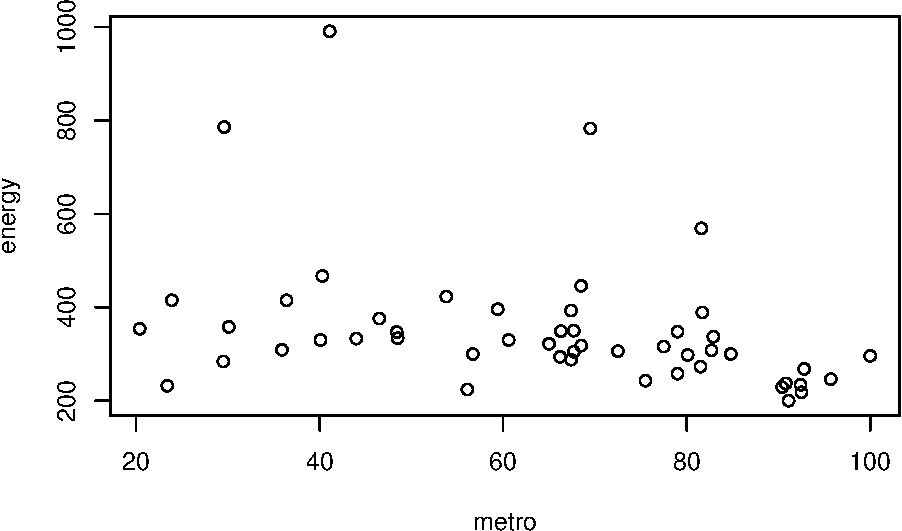
\includegraphics{R/Rmodels/figures/unnamed-chunk-126-1.pdf}

\begin{Shaded}
\begin{Highlighting}[]
  \KeywordTok{cor}\NormalTok{(states_en_met, }\DataTypeTok{use =} \StringTok{"pairwise"}\NormalTok{)}
\end{Highlighting}
\end{Shaded}

\begin{verbatim}
##            metro    energy
## metro   1.000000 -0.339745
## energy -0.339745  1.000000
\end{verbatim}

\begin{enumerate}
\def\labelenumi{\arabic{enumi}.}
\setcounter{enumi}{1}
\tightlist
\item
  Print and interpret the model \texttt{summary()}.
\end{enumerate}

\begin{Shaded}
\begin{Highlighting}[]
\NormalTok{  mod_en_met <-}\StringTok{ }\KeywordTok{lm}\NormalTok{(energy }\OperatorTok{~}\StringTok{ }\NormalTok{metro, }\DataTypeTok{data =}\NormalTok{ states)}
  \KeywordTok{summary}\NormalTok{(mod_en_met)}
\end{Highlighting}
\end{Shaded}

\begin{verbatim}
## 
## Call:
## lm(formula = energy ~ metro, data = states)
## 
## Residuals:
##    Min     1Q Median     3Q    Max 
## -215.5  -64.5  -30.9   18.7  584.0 
## 
## Coefficients:
##             Estimate Std. Error t value      Pr(>|t|)
## (Intercept)  501.029     61.814    8.11 0.00000000015
## metro         -2.287      0.914   -2.50         0.016
## 
## Residual standard error: 140 on 48 degrees of freedom
##   (1 observation deleted due to missingness)
## Multiple R-squared:  0.115,  Adjusted R-squared:  0.097 
## F-statistic: 6.26 on 1 and 48 DF,  p-value: 0.0158
\end{verbatim}

\begin{enumerate}
\def\labelenumi{\arabic{enumi}.}
\setcounter{enumi}{2}
\tightlist
\item
  \texttt{plot()} the model to look for deviations from modeling
  assumptions.
\end{enumerate}

\begin{Shaded}
\begin{Highlighting}[]
  \KeywordTok{plot}\NormalTok{(mod_en_met)}
\end{Highlighting}
\end{Shaded}

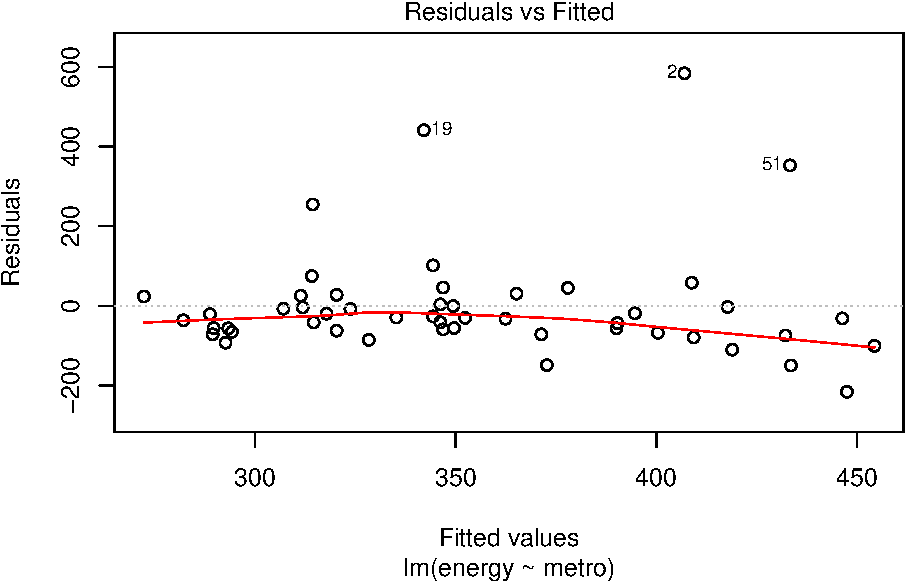
\includegraphics{R/Rmodels/figures/unnamed-chunk-128-1.pdf}
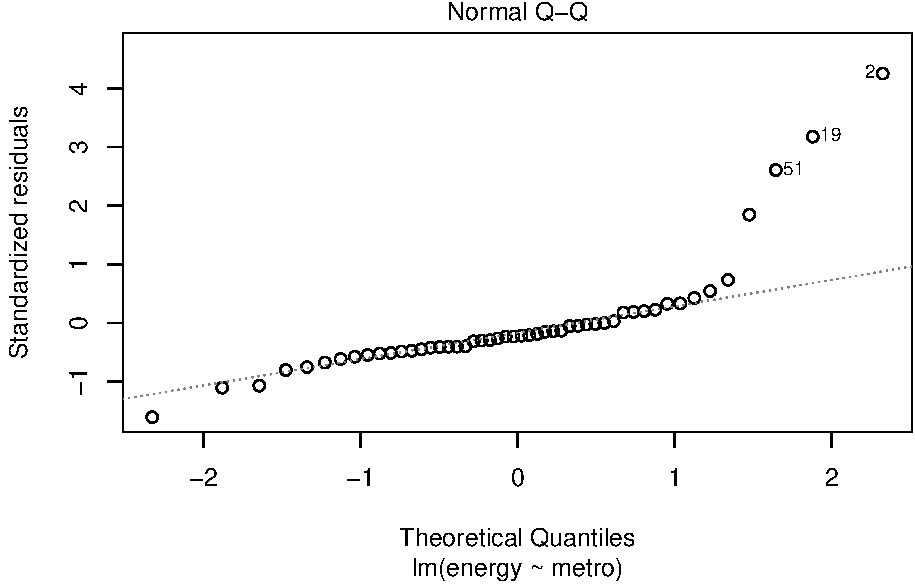
\includegraphics{R/Rmodels/figures/unnamed-chunk-128-2.pdf}
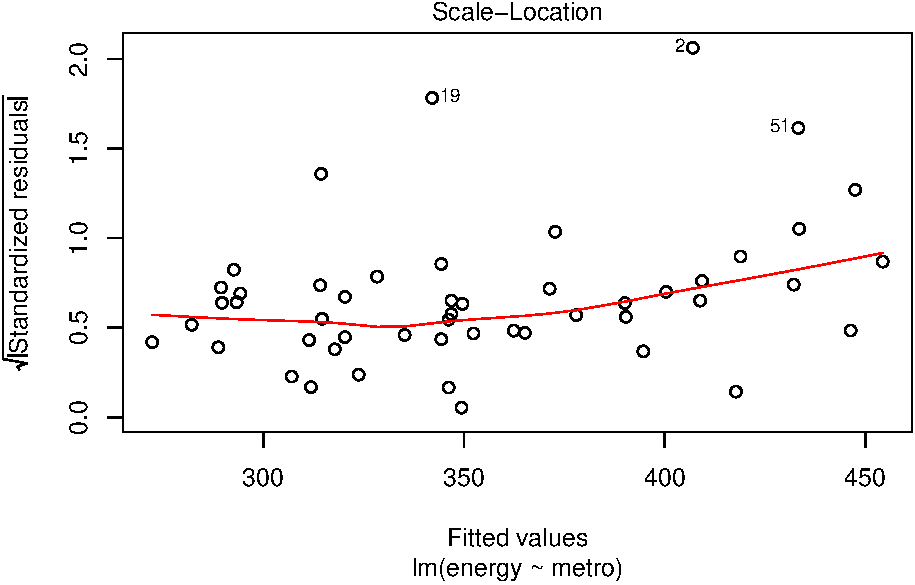
\includegraphics{R/Rmodels/figures/unnamed-chunk-128-3.pdf}
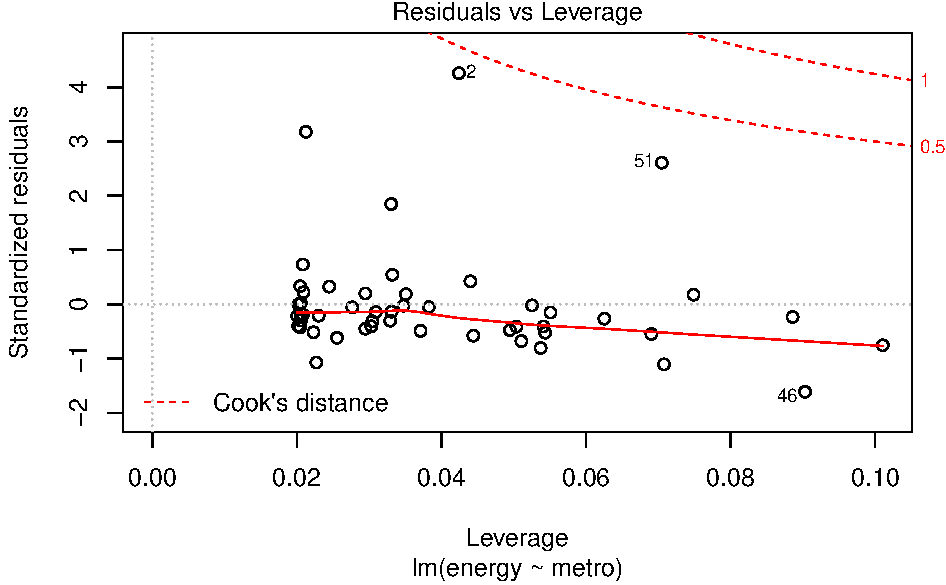
\includegraphics{R/Rmodels/figures/unnamed-chunk-128-4.pdf}

\begin{enumerate}
\def\labelenumi{\arabic{enumi}.}
\setcounter{enumi}{3}
\tightlist
\item
  Select one or more additional predictors to add to your model and
  repeat steps 1-3. Is this model significantly better than the model
  with \emph{metro} as the only predictor?
\end{enumerate}

\begin{Shaded}
\begin{Highlighting}[]
\NormalTok{  states_en_met_pop_wst <-}\StringTok{ }\KeywordTok{subset}\NormalTok{(states, }\DataTypeTok{select =} \KeywordTok{c}\NormalTok{(}\StringTok{"energy"}\NormalTok{, }\StringTok{"metro"}\NormalTok{, }\StringTok{"pop"}\NormalTok{, }\StringTok{"waste"}\NormalTok{))}
  \KeywordTok{summary}\NormalTok{(states_en_met_pop_wst)}
\end{Highlighting}
\end{Shaded}

\begin{verbatim}
##      energy        metro            pop               waste      
##  Min.   :200   Min.   : 20.4   Min.   :  454000   Min.   :0.540  
##  1st Qu.:285   1st Qu.: 47.0   1st Qu.: 1299750   1st Qu.:0.823  
##  Median :320   Median : 67.5   Median : 3390500   Median :0.960  
##  Mean   :354   Mean   : 64.1   Mean   : 4962040   Mean   :0.989  
##  3rd Qu.:372   3rd Qu.: 81.6   3rd Qu.: 5898000   3rd Qu.:1.145  
##  Max.   :991   Max.   :100.0   Max.   :29760000   Max.   :1.510  
##  NA's   :1     NA's   :1       NA's   :1          NA's   :1
\end{verbatim}

\begin{Shaded}
\begin{Highlighting}[]
  \KeywordTok{plot}\NormalTok{(states_en_met_pop_wst)}
\end{Highlighting}
\end{Shaded}

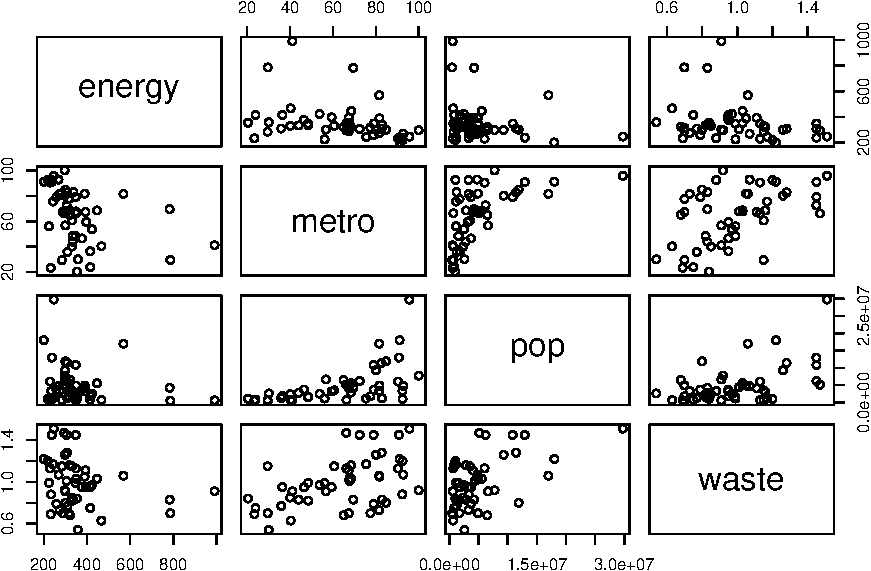
\includegraphics{R/Rmodels/figures/unnamed-chunk-129-1.pdf}

\begin{Shaded}
\begin{Highlighting}[]
  \KeywordTok{cor}\NormalTok{(states_en_met_pop_wst, }\DataTypeTok{use =} \StringTok{"pairwise"}\NormalTok{)}
\end{Highlighting}
\end{Shaded}

\begin{verbatim}
##           energy     metro       pop     waste
## energy  1.000000 -0.339745 -0.184036 -0.252650
## metro  -0.339745  1.000000  0.565356  0.487788
## pop    -0.184036  0.565356  1.000000  0.525571
## waste  -0.252650  0.487788  0.525571  1.000000
\end{verbatim}

\begin{Shaded}
\begin{Highlighting}[]
\NormalTok{  mod_en_met_pop_waste <-}\StringTok{ }\KeywordTok{lm}\NormalTok{(energy }\OperatorTok{~}\StringTok{ }\DecValTok{1} \OperatorTok{+}\StringTok{ }\NormalTok{metro }\OperatorTok{+}\StringTok{ }\NormalTok{pop }\OperatorTok{+}\StringTok{ }\NormalTok{waste, }\DataTypeTok{data =}\NormalTok{ states)}
  \KeywordTok{summary}\NormalTok{(mod_en_met_pop_waste)}
\end{Highlighting}
\end{Shaded}

\begin{verbatim}
## 
## Call:
## lm(formula = energy ~ 1 + metro + pop + waste, data = states)
## 
## Residuals:
##    Min     1Q Median     3Q    Max 
## -224.6  -67.5  -31.8   12.7  589.5 
## 
## Coefficients:
##                 Estimate   Std. Error t value  Pr(>|t|)
## (Intercept) 561.66773812  99.04681924    5.67 0.0000009
## metro        -2.07914840   1.16786868   -1.78     0.082
## pop           0.00000165   0.00000481    0.34     0.733
## waste       -83.07494970 104.21963267   -0.80     0.429
## 
## Residual standard error: 142 on 46 degrees of freedom
##   (1 observation deleted due to missingness)
## Multiple R-squared:  0.128,  Adjusted R-squared:  0.0707 
## F-statistic: 2.24 on 3 and 46 DF,  p-value: 0.096
\end{verbatim}

\begin{Shaded}
\begin{Highlighting}[]
  \KeywordTok{anova}\NormalTok{(mod_en_met, mod_en_met_pop_waste)}
\end{Highlighting}
\end{Shaded}

\begin{verbatim}
## Analysis of Variance Table
## 
## Model 1: energy ~ metro
## Model 2: energy ~ 1 + metro + pop + waste
##   Res.Df    RSS Df Sum of Sq    F Pr(>F)
## 1     48 943103                         
## 2     46 930153  2     12949 0.32  0.728
\end{verbatim}

\subsection{Ex 1: prototype}\label{ex-1-prototype-1}

Use the states data set.

\begin{enumerate}
\def\labelenumi{\arabic{enumi}.}
\tightlist
\item
  Add on to the regression equation that you created in exercise 1 by
  generating an interaction term and testing the interaction.
\end{enumerate}

\begin{Shaded}
\begin{Highlighting}[]
\NormalTok{  mod_en_metro_by_waste <-}\StringTok{ }\KeywordTok{lm}\NormalTok{(energy }\OperatorTok{~}\StringTok{ }\DecValTok{1} \OperatorTok{+}\StringTok{ }\NormalTok{metro }\OperatorTok{*}\StringTok{ }\NormalTok{waste, }\DataTypeTok{data =}\NormalTok{ states)}
\end{Highlighting}
\end{Shaded}

\begin{enumerate}
\def\labelenumi{\arabic{enumi}.}
\setcounter{enumi}{1}
\tightlist
\item
  Try adding a region to the model. Are there significant differences
  across the four regions?
\end{enumerate}

\begin{Shaded}
\begin{Highlighting}[]
\NormalTok{  mod_en_region <-}\StringTok{ }\KeywordTok{lm}\NormalTok{(energy }\OperatorTok{~}\StringTok{ }\DecValTok{1} \OperatorTok{+}\StringTok{ }\NormalTok{metro }\OperatorTok{*}\StringTok{ }\NormalTok{waste }\OperatorTok{+}\StringTok{ }\NormalTok{region, }\DataTypeTok{data =}\NormalTok{ states)}
  \KeywordTok{anova}\NormalTok{(mod_en_region)}
\end{Highlighting}
\end{Shaded}

\begin{verbatim}
## Analysis of Variance Table
## 
## Response: energy
##             Df Sum Sq Mean Sq F value Pr(>F)
## metro        1 123064  123064   6.444 0.0148
## waste        1  10572   10572   0.554 0.4609
## region       3 111128   37043   1.940 0.1375
## metro:waste  1    156     156   0.008 0.9284
## Residuals   43 821247   19099
\end{verbatim}

\subsection{Ex 2: prototype}\label{ex-2-prototype}

Use the NH11 data set that we loaded earlier. Note that the data is not
perfectly clean and ready to be modeled. You will need to clean up at
least some of the variables before fitting the model.

\begin{enumerate}
\def\labelenumi{\arabic{enumi}.}
\tightlist
\item
  Use \texttt{glm()} to conduct a logistic regression to predict ever
  worked (\texttt{everwrk}) using age (\texttt{age\_p}) and marital
  status (\texttt{r\_maritl}). Make sure you only keep the following two
  levels for \texttt{everwrk} (\texttt{1\ Yes} and \texttt{2\ No}).
  Hint: use the \texttt{factor()} function. Also, make sure to drop any
  \texttt{r\_maritl} levels that do not contain observations. Hint: see
  \texttt{?droplevels}.
\end{enumerate}

\begin{Shaded}
\begin{Highlighting}[]
\NormalTok{  NH11 <-}\StringTok{ }\KeywordTok{mutate}\NormalTok{(NH11,}
                     \DataTypeTok{everwrk =} \KeywordTok{factor}\NormalTok{(everwrk, }\DataTypeTok{levels =} \KeywordTok{c}\NormalTok{(}\StringTok{"1 Yes"}\NormalTok{, }\StringTok{"2 No"}\NormalTok{)),}
                     \DataTypeTok{r_maritl =} \KeywordTok{droplevels}\NormalTok{(r_maritl))}

\NormalTok{  mod_wk_age_mar <-}\StringTok{ }\KeywordTok{glm}\NormalTok{(everwrk }\OperatorTok{~}\StringTok{ }\DecValTok{1} \OperatorTok{+}\StringTok{ }\NormalTok{age_p }\OperatorTok{+}\StringTok{ }\NormalTok{r_maritl, }
                        \DataTypeTok{data =}\NormalTok{ NH11,}
                        \DataTypeTok{family =} \KeywordTok{binomial}\NormalTok{(}\DataTypeTok{link =} \StringTok{"logit"}\NormalTok{))}

  \KeywordTok{summary}\NormalTok{(mod_wk_age_mar)}
\end{Highlighting}
\end{Shaded}

\begin{verbatim}
## 
## Call:
## glm(formula = everwrk ~ 1 + age_p + r_maritl, family = binomial(link = "logit"), 
##     data = NH11)
## 
## Deviance Residuals: 
##    Min      1Q  Median      3Q     Max  
## -1.044  -0.565  -0.439  -0.337   2.731  
## 
## Coefficients:
##                                             Estimate Std. Error z value            Pr(>|z|)
## (Intercept)                                 -0.44025    0.09354   -4.71 0.00000251841905292
## age_p                                       -0.02981    0.00165  -18.12             < 2e-16
## r_maritl2 Married - spouse not in household  0.04968    0.21731    0.23              0.8192
## r_maritl4 Widowed                            0.68362    0.08434    8.11 0.00000000000000052
## r_maritl5 Divorced                          -0.73011    0.11168   -6.54 0.00000000006254929
## r_maritl6 Separated                         -0.12809    0.15137   -0.85              0.3974
## r_maritl7 Never married                      0.34361    0.06922    4.96 0.00000069100229497
## r_maritl8 Living with partner               -0.44358    0.13777   -3.22              0.0013
## r_maritl9 Unknown marital status             0.39548    0.49297    0.80              0.4224
## 
## (Dispersion parameter for binomial family taken to be 1)
## 
##     Null deviance: 11082  on 14039  degrees of freedom
## Residual deviance: 10309  on 14031  degrees of freedom
##   (18974 observations deleted due to missingness)
## AIC: 10327
## 
## Number of Fisher Scoring iterations: 5
\end{verbatim}

\begin{enumerate}
\def\labelenumi{\arabic{enumi}.}
\setcounter{enumi}{1}
\tightlist
\item
  Predict the probability of working for each level of marital status.
  Hint: use \texttt{allEffects()}.
\end{enumerate}

\begin{Shaded}
\begin{Highlighting}[]
\NormalTok{  eff <-}\StringTok{ }\KeywordTok{allEffects}\NormalTok{(mod_wk_age_mar)}
  \KeywordTok{as.data.frame}\NormalTok{(eff)}
\end{Highlighting}
\end{Shaded}

\begin{verbatim}
## $age_p
##   age_p       fit         se     lower     upper
## 1    20 0.2758744 0.01144854 0.2540091 0.2988678
## 2    30 0.2204336 0.00748365 0.2061163 0.2354505
## 3    50 0.1347747 0.00318375 0.1286557 0.1411376
## 4    70 0.0790279 0.00305362 0.0732463 0.0852239
## 5    80 0.0598752 0.00312393 0.0540376 0.0662991
## 
## $r_maritl
##                              r_maritl       fit         se     lower     upper
## 1     1 Married - spouse in household 0.1082200 0.00425964 0.1001498 0.1168561
## 2 2 Married - spouse not in household 0.1131082 0.02139317 0.0774606 0.1622753
## 3                           4 Widowed 0.1938109 0.01063476 0.1738136 0.2155087
## 4                          5 Divorced 0.0552439 0.00536166 0.0456288 0.0667436
## 5                         6 Separated 0.0964642 0.01270750 0.0742682 0.1244022
## 6                     7 Never married 0.1461100 0.00745921 0.1320878 0.1613441
## 7               8 Living with partner 0.0722496 0.00890495 0.0566247 0.0917666
## 8            9 Unknown marital status 0.1527008 0.06352845 0.0644084 0.3205573
\end{verbatim}

\subsection{Ex 3: prototype}\label{ex-3-prototype-1}

Use the dataset, bh1996:

\begin{Shaded}
\begin{Highlighting}[]
  \KeywordTok{data}\NormalTok{(bh1996, }\DataTypeTok{package=}\StringTok{"multilevel"}\NormalTok{)}
\end{Highlighting}
\end{Shaded}

From the data documentation:

\begin{quote}
Variables are Leadership Climate (\texttt{LEAD}), Well-Being
(\texttt{WBEING}), and Work Hours (\texttt{HRS}). The group identifier
is named \texttt{GRP}.
\end{quote}

\begin{enumerate}
\def\labelenumi{\arabic{enumi}.}
\tightlist
\item
  Create a null model predicting wellbeing (\texttt{WBEING}).
\end{enumerate}

\begin{Shaded}
\begin{Highlighting}[]
\NormalTok{  mod_grp0 <-}\StringTok{ }\KeywordTok{lmer}\NormalTok{(WBEING }\OperatorTok{~}\StringTok{ }\DecValTok{1} \OperatorTok{+}\StringTok{ }\NormalTok{(}\DecValTok{1} \OperatorTok{|}\StringTok{ }\NormalTok{GRP), }\DataTypeTok{data =}\NormalTok{ bh1996)}
  \KeywordTok{summary}\NormalTok{(mod_grp0)}
\end{Highlighting}
\end{Shaded}

\begin{verbatim}
## Linear mixed model fit by REML ['lmerMod']
## Formula: WBEING ~ 1 + (1 | GRP)
##    Data: bh1996
## 
## REML criterion at convergence: 19347.3
## 
## Scaled residuals: 
##    Min     1Q Median     3Q    Max 
## -3.322 -0.648  0.031  0.718  2.667 
## 
## Random effects:
##  Groups   Name        Variance Std.Dev.
##  GRP      (Intercept) 0.0358   0.189   
##  Residual             0.7895   0.889   
## Number of obs: 7382, groups:  GRP, 99
## 
## Fixed effects:
##             Estimate Std. Error t value
## (Intercept)   2.7743     0.0222     125
\end{verbatim}

\begin{enumerate}
\def\labelenumi{\arabic{enumi}.}
\setcounter{enumi}{2}
\tightlist
\item
  Run a second multi-level model that adds two individual-level
  predictors, average number of hours worked (\texttt{HRS}) and
  leadership skills (\texttt{LEAD}) to the model and interpret your
  output.
\end{enumerate}

\begin{Shaded}
\begin{Highlighting}[]
\NormalTok{  mod_grp1 <-}\StringTok{ }\KeywordTok{lmer}\NormalTok{(WBEING }\OperatorTok{~}\StringTok{ }\DecValTok{1} \OperatorTok{+}\StringTok{ }\NormalTok{HRS }\OperatorTok{+}\StringTok{ }\NormalTok{LEAD }\OperatorTok{+}\StringTok{ }\NormalTok{(}\DecValTok{1} \OperatorTok{|}\StringTok{ }\NormalTok{GRP), }\DataTypeTok{data =}\NormalTok{ bh1996)}
  \KeywordTok{summary}\NormalTok{(mod_grp1)}
\end{Highlighting}
\end{Shaded}

\begin{verbatim}
## Linear mixed model fit by REML ['lmerMod']
## Formula: WBEING ~ 1 + HRS + LEAD + (1 | GRP)
##    Data: bh1996
## 
## REML criterion at convergence: 17860
## 
## Scaled residuals: 
##    Min     1Q Median     3Q    Max 
## -3.919 -0.659  0.038  0.704  3.644 
## 
## Random effects:
##  Groups   Name        Variance Std.Dev.
##  GRP      (Intercept) 0.0193   0.139   
##  Residual             0.6467   0.804   
## Number of obs: 7382, groups:  GRP, 99
## 
## Fixed effects:
##             Estimate Std. Error t value
## (Intercept)  1.68616    0.06770   24.91
## HRS         -0.03162    0.00438   -7.22
## LEAD         0.50074    0.01281   39.09
## 
## Correlation of Fixed Effects:
##      (Intr) HRS   
## HRS  -0.800       
## LEAD -0.635  0.121
\end{verbatim}

\begin{enumerate}
\def\labelenumi{\arabic{enumi}.}
\setcounter{enumi}{2}
\tightlist
\item
  Now, add a random effect of average number of hours worked
  (\texttt{HRS}) to the model and interpret your output. Test the
  significance of this random term.
\end{enumerate}

\begin{Shaded}
\begin{Highlighting}[]
\NormalTok{  mod_grp2 <-}\StringTok{ }\KeywordTok{lmer}\NormalTok{(WBEING }\OperatorTok{~}\StringTok{ }\DecValTok{1} \OperatorTok{+}\StringTok{ }\NormalTok{HRS }\OperatorTok{+}\StringTok{ }\NormalTok{LEAD }\OperatorTok{+}\StringTok{ }\NormalTok{(}\DecValTok{1} \OperatorTok{+}\StringTok{ }\NormalTok{HRS }\OperatorTok{|}\StringTok{ }\NormalTok{GRP), }\DataTypeTok{data =}\NormalTok{ bh1996)}
  \KeywordTok{anova}\NormalTok{(mod_grp1, mod_grp2)}
\end{Highlighting}
\end{Shaded}

\begin{verbatim}
## Data: bh1996
## Models:
## mod_grp1: WBEING ~ 1 + HRS + LEAD + (1 | GRP)
## mod_grp2: WBEING ~ 1 + HRS + LEAD + (1 + HRS | GRP)
##          Df   AIC   BIC logLik deviance Chisq Chi Df Pr(>Chisq)
## mod_grp1  5 17848 17882  -8919    17838                        
## mod_grp2  7 17851 17899  -8918    17837  1.22      2      0.543
\end{verbatim}

\section{Wrap-up}\label{wrap-up-2}

\subsection{Feedback}\label{feedback-2}

These workshops are a work in progress, please provide any feedback to:
\href{mailto:help@iq.harvard.edu}{\nolinkurl{help@iq.harvard.edu}}

\subsection{Resources}\label{resources-3}

\begin{itemize}
\tightlist
\item
  IQSS

  \begin{itemize}
  \tightlist
  \item
    Workshops: \url{https://dss.iq.harvard.edu/workshop-materials}
  \item
    Data Science Services: \url{https://dss.iq.harvard.edu/}
  \item
    Research Computing Environment:
    \url{https://iqss.github.io/dss-rce/}
  \end{itemize}
\item
  HBS

  \begin{itemize}
  \tightlist
  \item
    Research Computing Services workshops:
    \url{https://training.rcs.hbs.org/workshops}
  \item
    Other HBS RCS resources:
    \url{https://training.rcs.hbs.org/workshop-materials}
  \item
    RCS consulting email: \url{mailto:research@hbs.edu}
  \end{itemize}
\end{itemize}

\chapter{R Graphics}\label{r-graphics}

\textbf{Topics}

\begin{itemize}
\tightlist
\item
  R \texttt{ggplot2} package
\item
  Geometric objects and aesthetics
\item
  Setup basic plots
\item
  Add and modify scales and legends
\item
  Manipulate plot labels
\item
  Change and create plot themes
\end{itemize}

\section{Setup}\label{setup-2}

\subsection{Class Structure}\label{class-structure-2}

\begin{itemize}
\tightlist
\item
  Informal --- Ask questions at any time. Really!
\item
  Collaboration is encouraged - please spend a minute introducing
  yourself to your neighbors!
\end{itemize}

\subsection{Prerequisites}\label{prerequisites-2}

This is an intermediate R course:

\begin{itemize}
\tightlist
\item
  Assumes working knowledge of R
\item
  Relatively fast-paced
\end{itemize}

\subsection{Launch an R session}\label{launch-an-r-session-1}

Start RStudio and create a new project:

\begin{itemize}
\tightlist
\item
  On Windows click the start button and search for RStudio. On Mac
  RStudio will be in your applications folder.
\item
  In Rstudio go to \texttt{File\ -\textgreater{}\ New\ Project}.
\item
  Choose \texttt{Existing\ Directory} and browse to the workshop
  materials directory on your desktop.
\item
  Choose \texttt{File\ -\textgreater{}\ Open\ File} and select the file
  with the word ``BLANK'' in the name.
\end{itemize}

\subsection{Packages}\label{packages-1}

You should have already installed the \texttt{tidyverse} and
\texttt{rmarkdown} packages onto your computer before the workshop ---
see \href{./Rinstall.html}{R Installation}. Now let's load these
packages into the search path of our R session.

\begin{Shaded}
\begin{Highlighting}[]
\KeywordTok{library}\NormalTok{(tidyverse)}
\KeywordTok{library}\NormalTok{(rmarkdown)}
\end{Highlighting}
\end{Shaded}

The \texttt{ggplot2} package is contained within \texttt{tidyverse}, but
we also want to install two additional packages, \texttt{scales} and
\texttt{ggrepel}, which provide additional functionality.

\begin{Shaded}
\begin{Highlighting}[]
\CommentTok{# install.packages("scales")}
\KeywordTok{library}\NormalTok{(scales)}

\CommentTok{# install.packages("ggrepel") }
\KeywordTok{library}\NormalTok{(ggrepel)}
\end{Highlighting}
\end{Shaded}

\subsection{Goals}\label{goals-2}

We will learn about the \texttt{grammar\ of\ graphics} --- a system for
understanding the building blocks of a graph --- using the
\texttt{ggplot2} package. In particular, we'll learn about:

\begin{enumerate}
\def\labelenumi{\arabic{enumi}.}
\tightlist
\item
  Basic plots, \textbf{aesthetic mapping and inheritance}
\item
  Tailoring \textbf{statistical transformations} to particular plots
\item
  \textbf{Modifying scales} to change axes and add labels
\item
  \textbf{Faceting} to create many small plots
\item
  Changing plot \textbf{themes}
\end{enumerate}

\section{\texorpdfstring{Why
\texttt{ggplot2}?}{Why ggplot2?}}\label{why-ggplot2}

\texttt{ggplot2} is a package within in the \texttt{tidyverse} suite of
packages. Advantages of \texttt{ggplot2} include:

\begin{itemize}
\tightlist
\item
  consistent underlying \texttt{grammar\ of\ graphics} (Wilkinson, 2005)
\item
  very flexible --- plot specification at a high level of abstraction
\item
  theme system for polishing plot appearance
\item
  many users, active mailing list
\end{itemize}

That said, there are some things you cannot (or should not) do with
\texttt{ggplot2}:

\begin{itemize}
\tightlist
\item
  3-dimensional graphics (see the \texttt{rgl} package)
\item
  Graph-theory type graphs (nodes/edges layout; see the \texttt{igraph}
  package)
\item
  Interactive graphics (see the \texttt{ggvis} package)
\end{itemize}

\subsection{What is the Grammar Of
Graphics?}\label{what-is-the-grammar-of-graphics}

The basic idea: independently specify plot building blocks and combine
them to create just about any kind of graphical display you want.
Building blocks of a graph include the following (\textbf{bold denotes
essential elements}):

\begin{itemize}
\tightlist
\item
  \textbf{data}
\item
  \textbf{aesthetic mapping}
\item
  \textbf{geometric object}
\item
  statistical transformations
\item
  scales
\item
  coordinate system
\item
  position adjustments
\item
  faceting
\item
  themes
\end{itemize}

By the end of this workshop, you should understand what these building
blocks do and how to use them to create the following plot:

\begin{figure}
\centering
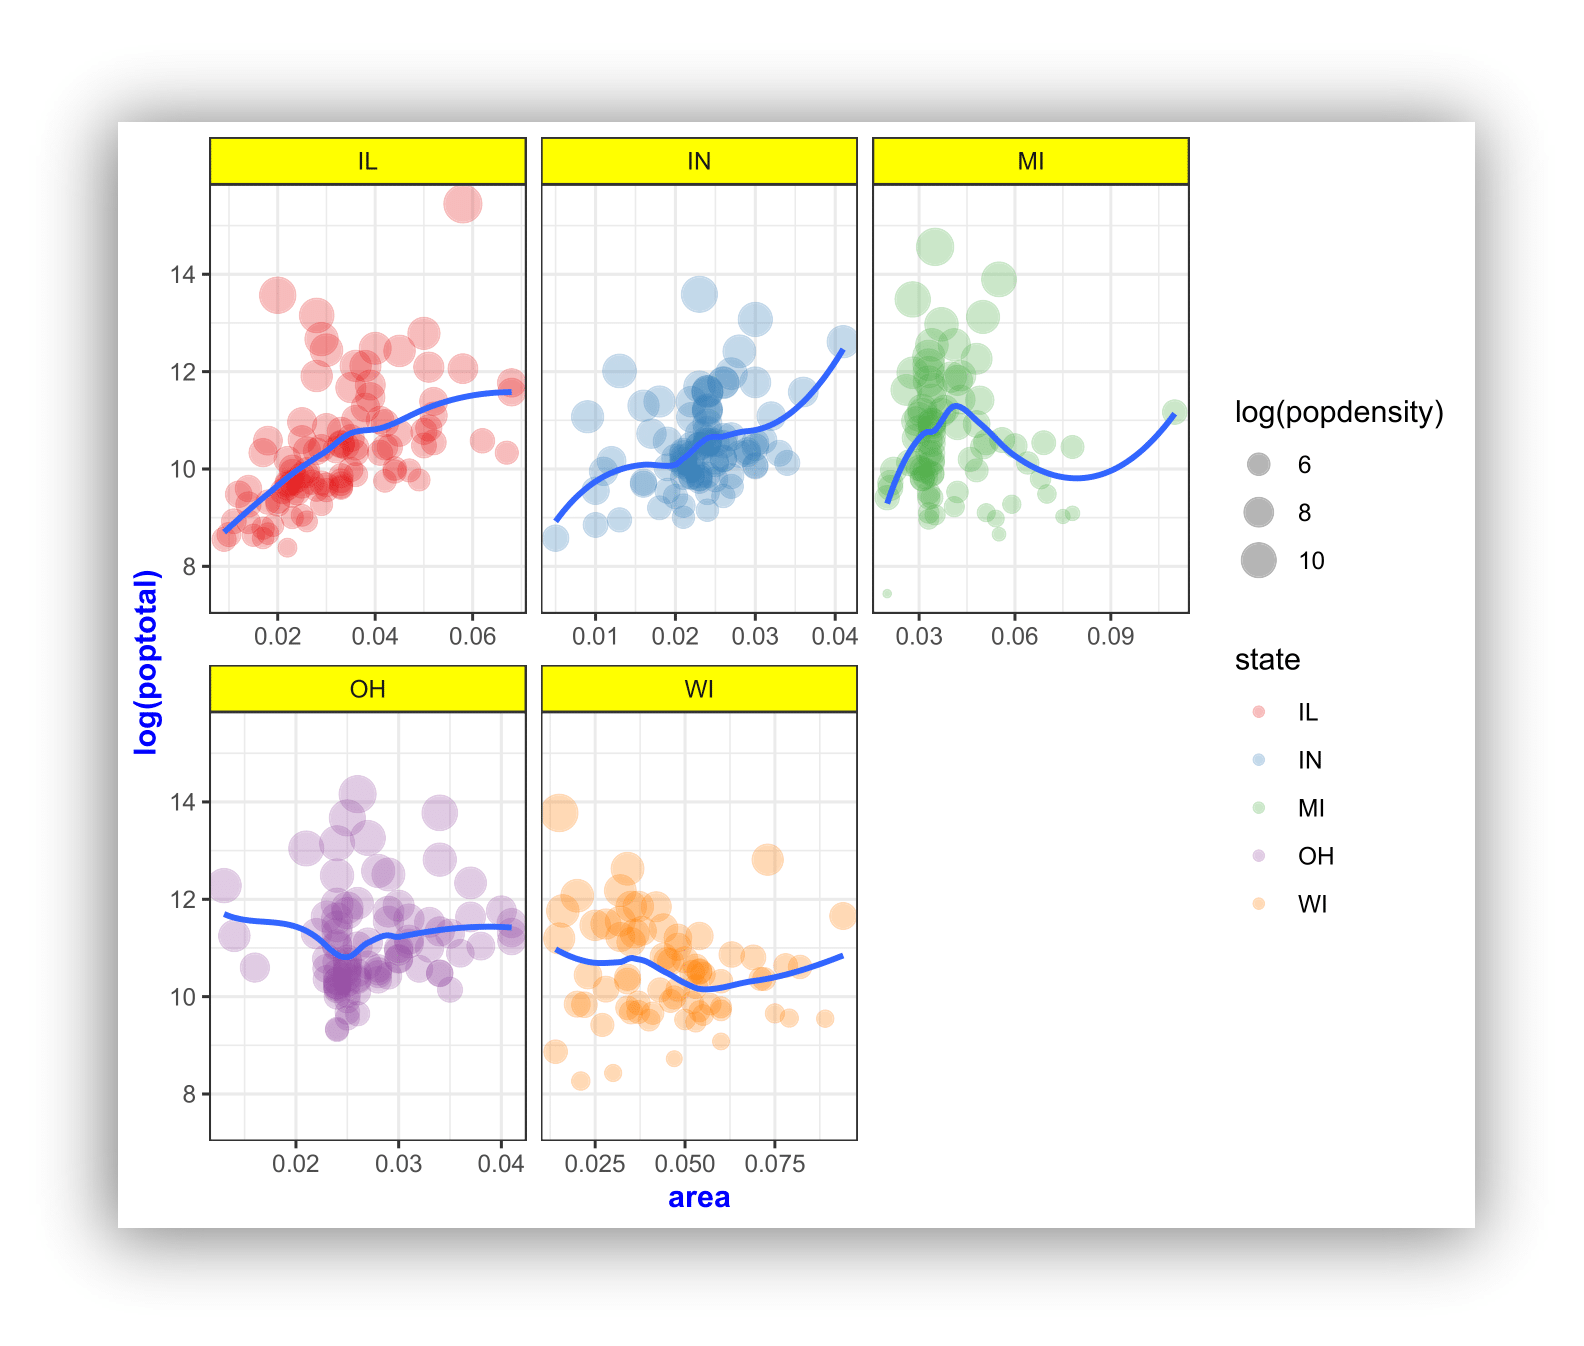
\includegraphics{R/Rgraphics/images/final_plot.png}
\caption{}
\end{figure}

\subsection{\texorpdfstring{\texttt{ggplot2} VS base
graphics}{ggplot2 VS base graphics}}\label{ggplot2-vs-base-graphics}

Compared to base graphics, \texttt{ggplot2}

\begin{itemize}
\tightlist
\item
  is more verbose for simple / canned graphics
\item
  is less verbose for complex / custom graphics
\item
  does not have methods (data should always be in a \texttt{data.frame})
\item
  has sensible defaults for generating legends
\end{itemize}

\section{Geometric objects \&
aesthetics}\label{geometric-objects-aesthetics}

\subsection{Aesthetic mapping}\label{aesthetic-mapping}

In ggplot land \emph{aesthetic} means ``something you can see''.
Examples include:

\begin{itemize}
\tightlist
\item
  position (i.e., on the x and y axes)
\item
  color (``outside'' color)
\item
  fill (``inside'' color)
\item
  shape (of points)
\item
  linetype
\item
  size
\end{itemize}

Each type of geom accepts only a subset of all aesthetics; refer to the
geom help pages to see what mappings each geom accepts. Aesthetic
mappings are set with the \texttt{aes()} function.

\subsection{\texorpdfstring{Geometric objects
(\texttt{geom})}{Geometric objects (geom)}}\label{geometric-objects-geom}

Geometric objects are the actual marks we put on a plot. Examples
include:

\begin{itemize}
\tightlist
\item
  points (\texttt{geom\_point()}, for scatter plots, dot plots, etc.)
\item
  lines (\texttt{geom\_line()}, for time series, trend lines, etc.)
\item
  boxplot (\texttt{geom\_boxplot()}, for boxplots!)
\end{itemize}

A plot \textbf{must have at least one geom}; there is no upper limit.
You can add a geom to a plot using the \texttt{+} operator.

Each \texttt{geom\_} has a particular set of aesthetic mappings
associated with it. Some examples are provided below, with required
aesthetics in \textbf{bold} and optional aesthetics in plain text:

\begin{longtable}[]{@{}lll@{}}
\toprule
\begin{minipage}[b]{0.13\columnwidth}\raggedright\strut
\texttt{geom\_}\strut
\end{minipage} & \begin{minipage}[b]{0.14\columnwidth}\raggedright\strut
Usage\strut
\end{minipage} & \begin{minipage}[b]{0.64\columnwidth}\raggedright\strut
Aesthetics\strut
\end{minipage}\tabularnewline
\midrule
\endhead
\begin{minipage}[t]{0.13\columnwidth}\raggedright\strut
\texttt{geom\_point()}\strut
\end{minipage} & \begin{minipage}[t]{0.14\columnwidth}\raggedright\strut
Scatter plot\strut
\end{minipage} & \begin{minipage}[t]{0.64\columnwidth}\raggedright\strut
\textbf{\texttt{x}},\textbf{\texttt{y}},\texttt{alpha},\texttt{color},\texttt{fill},\texttt{group},\texttt{shape},\texttt{size},\texttt{stroke}\strut
\end{minipage}\tabularnewline
\begin{minipage}[t]{0.13\columnwidth}\raggedright\strut
\texttt{geom\_line()}\strut
\end{minipage} & \begin{minipage}[t]{0.14\columnwidth}\raggedright\strut
Line plot\strut
\end{minipage} & \begin{minipage}[t]{0.64\columnwidth}\raggedright\strut
\textbf{\texttt{x}},\textbf{\texttt{y}},\texttt{alpha},\texttt{color},\texttt{linetype},\texttt{size}\strut
\end{minipage}\tabularnewline
\begin{minipage}[t]{0.13\columnwidth}\raggedright\strut
\texttt{geom\_bar()}\strut
\end{minipage} & \begin{minipage}[t]{0.14\columnwidth}\raggedright\strut
Bar chart\strut
\end{minipage} & \begin{minipage}[t]{0.64\columnwidth}\raggedright\strut
\textbf{\texttt{x}},\textbf{\texttt{y}},\texttt{alpha},\texttt{color},\texttt{fill},\texttt{group},\texttt{linetype},\texttt{size}\strut
\end{minipage}\tabularnewline
\begin{minipage}[t]{0.13\columnwidth}\raggedright\strut
\texttt{geom\_boxplot()}\strut
\end{minipage} & \begin{minipage}[t]{0.14\columnwidth}\raggedright\strut
Boxplot\strut
\end{minipage} & \begin{minipage}[t]{0.64\columnwidth}\raggedright\strut
\textbf{\texttt{x}},\textbf{\texttt{lower}},\textbf{\texttt{upper}},\textbf{\texttt{middle}},\textbf{\texttt{ymin}},\textbf{\texttt{ymax}},\texttt{alpha},\texttt{color},\texttt{fill}\strut
\end{minipage}\tabularnewline
\begin{minipage}[t]{0.13\columnwidth}\raggedright\strut
\texttt{geom\_density()}\strut
\end{minipage} & \begin{minipage}[t]{0.14\columnwidth}\raggedright\strut
Density plot\strut
\end{minipage} & \begin{minipage}[t]{0.64\columnwidth}\raggedright\strut
\textbf{\texttt{x}},\textbf{\texttt{y}},\texttt{alpha},\texttt{color},\texttt{fill},\texttt{group},\texttt{linetype},\texttt{size},\texttt{weight}\strut
\end{minipage}\tabularnewline
\begin{minipage}[t]{0.13\columnwidth}\raggedright\strut
\texttt{geom\_smooth()}\strut
\end{minipage} & \begin{minipage}[t]{0.14\columnwidth}\raggedright\strut
Conditional means\strut
\end{minipage} & \begin{minipage}[t]{0.64\columnwidth}\raggedright\strut
\textbf{\texttt{x}},\textbf{\texttt{y}},\texttt{alpha},\texttt{color},\texttt{fill},\texttt{group},\texttt{linetype},\texttt{size},\texttt{weight}\strut
\end{minipage}\tabularnewline
\begin{minipage}[t]{0.13\columnwidth}\raggedright\strut
\texttt{geom\_label()}\strut
\end{minipage} & \begin{minipage}[t]{0.14\columnwidth}\raggedright\strut
Text\strut
\end{minipage} & \begin{minipage}[t]{0.64\columnwidth}\raggedright\strut
\textbf{\texttt{x}},\textbf{\texttt{y}},\textbf{\texttt{label}},\texttt{alpha},\texttt{angle},\texttt{color},\texttt{family},\texttt{fontface},\texttt{size}\strut
\end{minipage}\tabularnewline
\bottomrule
\end{longtable}

You can get a list of all available geometric objects and their
associated aesthetics at \url{https://ggplot2.tidyverse.org/reference/}.
Or, simply type \texttt{geom\_\textless{}tab\textgreater{}} in any good
R IDE (such as Rstudio or ESS) to see a list of functions starting with
\texttt{geom\_}.

\subsubsection{Points (scatterplot)}\label{points-scatterplot}

Now that we know about geometric objects and aesthetic mapping, we can
make a \texttt{ggplot()}. \texttt{geom\_point()} requires mappings for x
and y, all others are optional.

\textbf{Example data: housing prices}

Let's look at housing prices.

\begin{Shaded}
\begin{Highlighting}[]
\NormalTok{housing <-}\StringTok{ }\KeywordTok{read_csv}\NormalTok{(}\StringTok{"dataSets/landdata-states.csv"}\NormalTok{)}
\KeywordTok{head}\NormalTok{(housing[}\DecValTok{1}\OperatorTok{:}\DecValTok{5}\NormalTok{])}
\end{Highlighting}
\end{Shaded}

\begin{verbatim}
## # A tibble: 6 x 5
##   State region  Date Home_Value Structure_Cost
##   <chr> <chr>  <dbl>      <dbl>          <dbl>
## 1 AK    West   2010.     224952         160599
## 2 AK    West   2010.     225511         160252
## 3 AK    West   2010.     225820         163791
## 4 AK    West   2010      224994         161787
## 5 AK    West   2008      234590         155400
## 6 AK    West   2008.     233714         157458
\end{verbatim}

\begin{Shaded}
\begin{Highlighting}[]
\CommentTok{# create a subset for 1st quarter 2001}
\NormalTok{hp2001Q1 <-}\StringTok{ }\KeywordTok{filter}\NormalTok{(housing, Date }\OperatorTok{==}\StringTok{ }\FloatTok{2001.25}\NormalTok{)}
\end{Highlighting}
\end{Shaded}

\textbf{Step 1:} create a blank canvas by specifying data:

\begin{Shaded}
\begin{Highlighting}[]
\KeywordTok{ggplot}\NormalTok{(}\DataTypeTok{data =}\NormalTok{ hp2001Q1)}
\end{Highlighting}
\end{Shaded}


\includegraphics{R/Rgraphics/figures/unnamed-chunk-142-1.pdf}

\textbf{Step 2:} specify aesthetic mappings (how you want to map
variables to visual aspects):

\begin{Shaded}
\begin{Highlighting}[]
\CommentTok{# here we map "Land_Value" and "Structure_Cost" to the x- and y-axes.}
\KeywordTok{ggplot}\NormalTok{(}\DataTypeTok{data =}\NormalTok{ hp2001Q1, }\DataTypeTok{mapping =} \KeywordTok{aes}\NormalTok{(}\DataTypeTok{x =}\NormalTok{ Land_Value, }\DataTypeTok{y =}\NormalTok{ Structure_Cost))}
\end{Highlighting}
\end{Shaded}

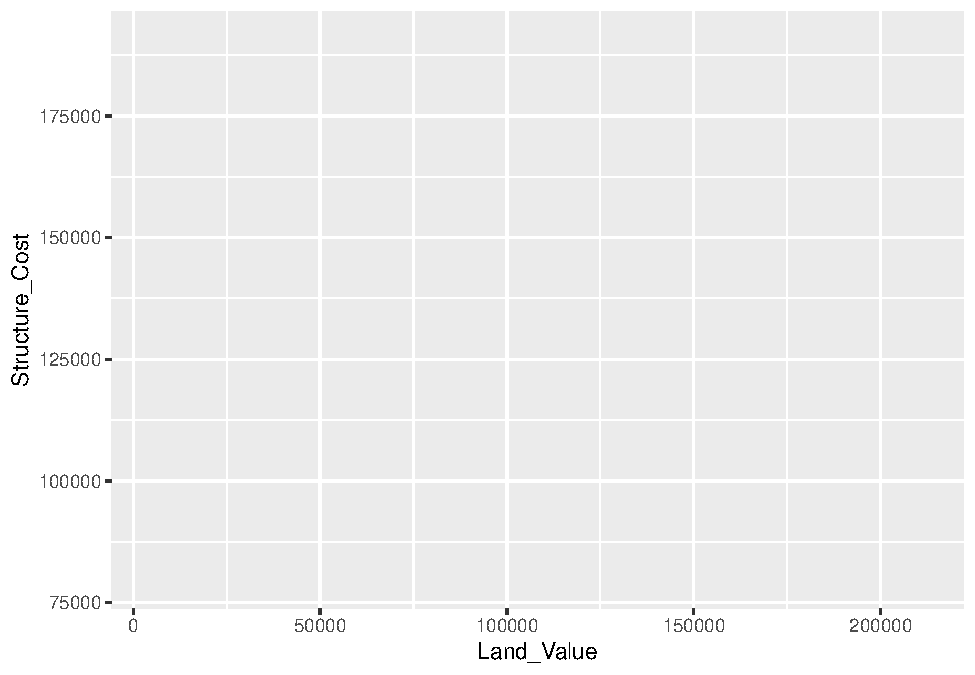
\includegraphics{R/Rgraphics/figures/unnamed-chunk-143-1.pdf}

\textbf{Step 3:} add new layers of geometric objects that will show up
on the plot:

\begin{Shaded}
\begin{Highlighting}[]
\CommentTok{# here we use geom_point() to add a layer with point (dot) elements }
\CommentTok{# as the geometric shapes to represent the data.}
\KeywordTok{ggplot}\NormalTok{(}\DataTypeTok{data =}\NormalTok{ hp2001Q1, }\DataTypeTok{mapping =} \KeywordTok{aes}\NormalTok{(}\DataTypeTok{x =}\NormalTok{ Land_Value, }\DataTypeTok{y =}\NormalTok{ Structure_Cost)) }\OperatorTok{+}
\StringTok{  }\KeywordTok{geom_point}\NormalTok{()}
\end{Highlighting}
\end{Shaded}


\includegraphics{R/Rgraphics/figures/unnamed-chunk-144-1.pdf}

\subsubsection{Lines (prediction line)}\label{lines-prediction-line}

A plot constructed with \texttt{ggplot()} can have more than one geom.
In that case the mappings established in the \texttt{ggplot()} call are
plot defaults that can be added to or overridden --- this is referred to
as \textbf{aesthetic inheritance}. Our plot could use a regression line:

\begin{Shaded}
\begin{Highlighting}[]
\CommentTok{# get predicted values from a linear regression}
\NormalTok{hp2001Q1}\OperatorTok{$}\NormalTok{pred_SC <-}\StringTok{ }\KeywordTok{lm}\NormalTok{(Structure_Cost }\OperatorTok{~}\StringTok{ }\KeywordTok{log}\NormalTok{(Land_Value), }\DataTypeTok{data =}\NormalTok{ hp2001Q1) }\OperatorTok
\StringTok{  }\KeywordTok{predict}\NormalTok{()}

\NormalTok{p1 <-}\StringTok{ }\KeywordTok{ggplot}\NormalTok{(hp2001Q1, }\KeywordTok{aes}\NormalTok{(}\DataTypeTok{x =} \KeywordTok{log}\NormalTok{(Land_Value), }\DataTypeTok{y =}\NormalTok{ Structure_Cost))}

\NormalTok{p1 }\OperatorTok{+}\StringTok{ }\KeywordTok{geom_point}\NormalTok{(}\KeywordTok{aes}\NormalTok{(}\DataTypeTok{color =}\NormalTok{ Home_Value)) }\OperatorTok{+}\StringTok{ }\CommentTok{# values for x and y are inherited from the ggplot() call above}
\StringTok{  }\KeywordTok{geom_line}\NormalTok{(}\KeywordTok{aes}\NormalTok{(}\DataTypeTok{y =}\NormalTok{ pred_SC)) }\CommentTok{# add predicted values to the plot overriding the y values from the ggplot() call above}
\end{Highlighting}
\end{Shaded}

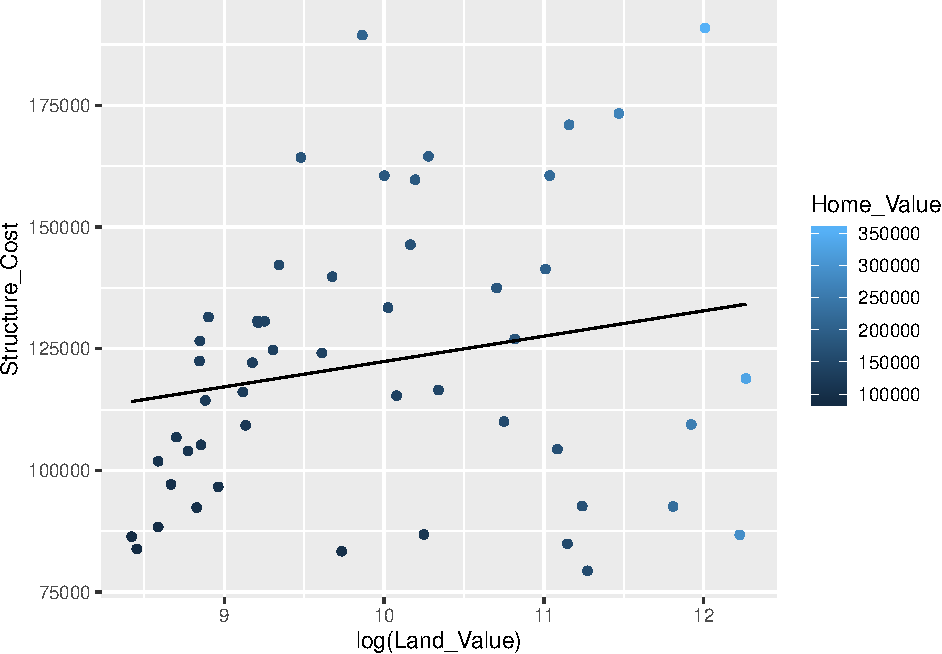
\includegraphics{R/Rgraphics/figures/unnamed-chunk-145-1.pdf}

\subsubsection{Smoothers}\label{smoothers}

Not all geometric objects are simple shapes; the smooth geom includes a
line and a ribbon.

\begin{Shaded}
\begin{Highlighting}[]
\NormalTok{p1 }\OperatorTok{+}
\StringTok{  }\KeywordTok{geom_point}\NormalTok{(}\KeywordTok{aes}\NormalTok{(}\DataTypeTok{color =}\NormalTok{ Home_Value)) }\OperatorTok{+}
\StringTok{  }\KeywordTok{geom_smooth}\NormalTok{()}
\end{Highlighting}
\end{Shaded}

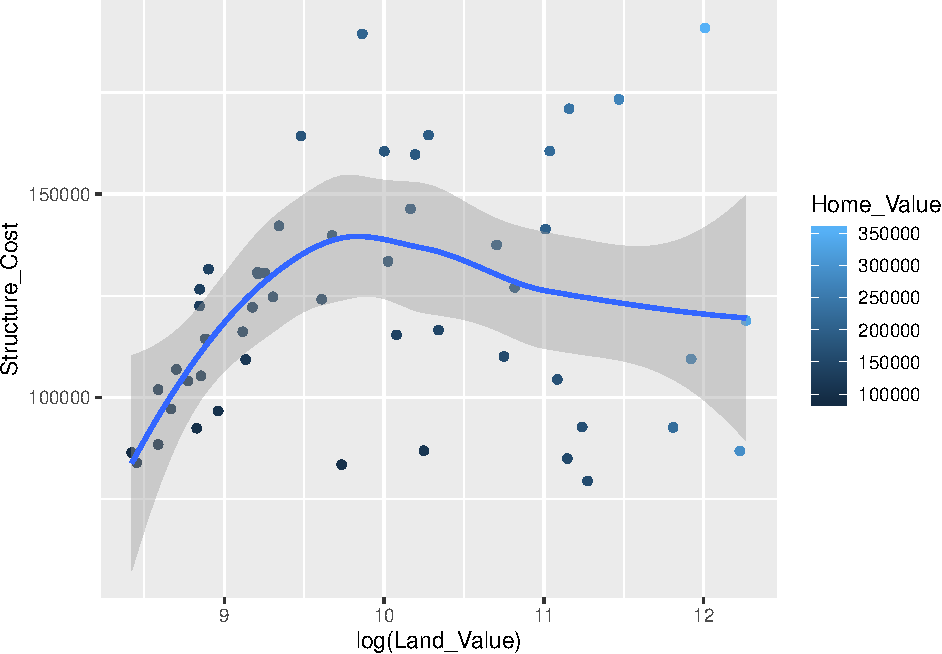
\includegraphics{R/Rgraphics/figures/unnamed-chunk-146-1.pdf}

\subsubsection{Text (label points)}\label{text-label-points}

Each geom accepts a particular set of mappings; for example
\texttt{geom\_text()} accepts a \texttt{label} mapping.

\begin{Shaded}
\begin{Highlighting}[]
\NormalTok{p1 }\OperatorTok{+}\StringTok{ }
\StringTok{  }\KeywordTok{geom_text}\NormalTok{(}\KeywordTok{aes}\NormalTok{(}\DataTypeTok{label=}\NormalTok{State), }\DataTypeTok{size =} \DecValTok{3}\NormalTok{)}
\end{Highlighting}
\end{Shaded}

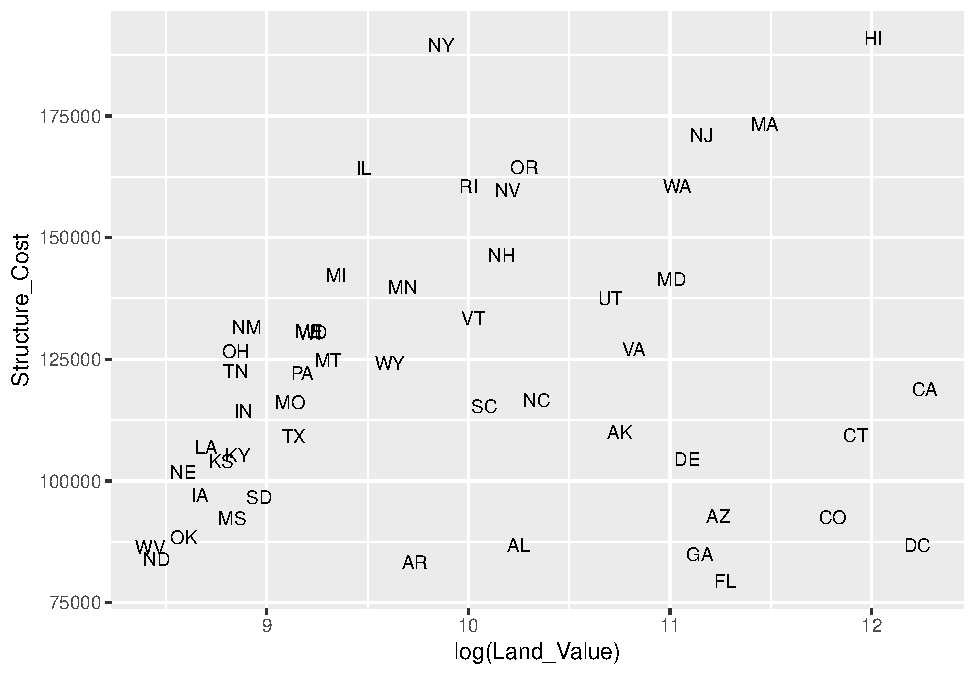
\includegraphics{R/Rgraphics/figures/unnamed-chunk-147-1.pdf}

\begin{Shaded}
\begin{Highlighting}[]
\NormalTok{p1 }\OperatorTok{+}\StringTok{ }
\StringTok{  }\KeywordTok{geom_point}\NormalTok{() }\OperatorTok{+}\StringTok{ }
\StringTok{  }\KeywordTok{geom_text_repel}\NormalTok{(}\KeywordTok{aes}\NormalTok{(}\DataTypeTok{label=}\NormalTok{State), }\DataTypeTok{size =} \DecValTok{3}\NormalTok{)}
\end{Highlighting}
\end{Shaded}

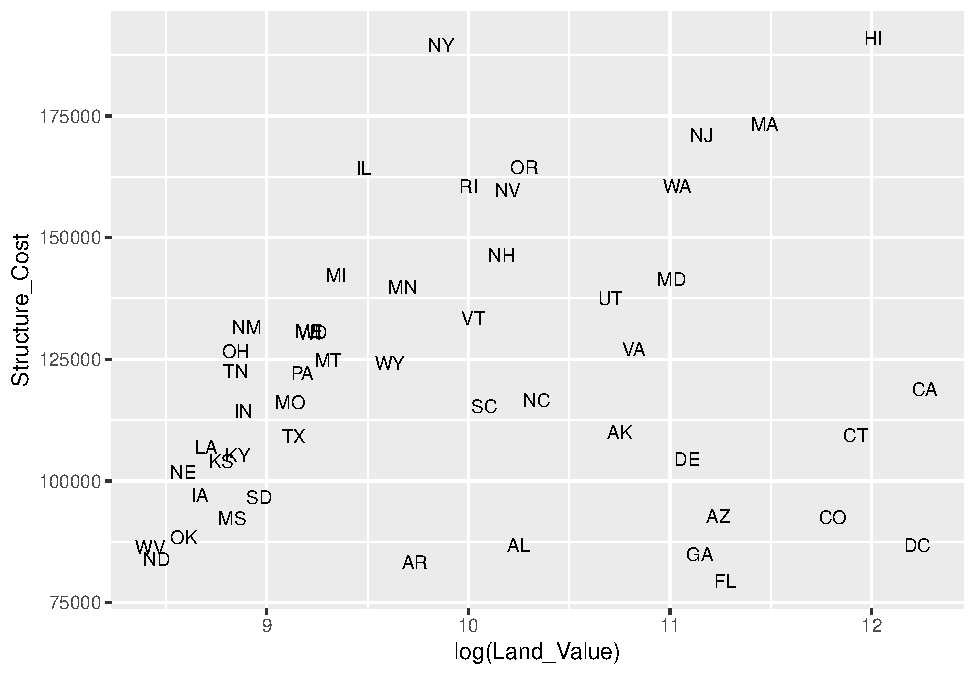
\includegraphics{R/Rgraphics/figures/unnamed-chunk-148-1.pdf}

\subsection{Aesthetic mapping VS
assignment}\label{aesthetic-mapping-vs-assignment}

\begin{enumerate}
\def\labelenumi{\arabic{enumi}.}
\tightlist
\item
  Variables are \textbf{mapped} to aesthetics within the \texttt{aes()}
  function
\end{enumerate}

\begin{Shaded}
\begin{Highlighting}[]
\NormalTok{p1 }\OperatorTok{+}
\StringTok{  }\KeywordTok{geom_point}\NormalTok{(}\KeywordTok{aes}\NormalTok{(}\DataTypeTok{size =}\NormalTok{ Home_Value))}
\end{Highlighting}
\end{Shaded}

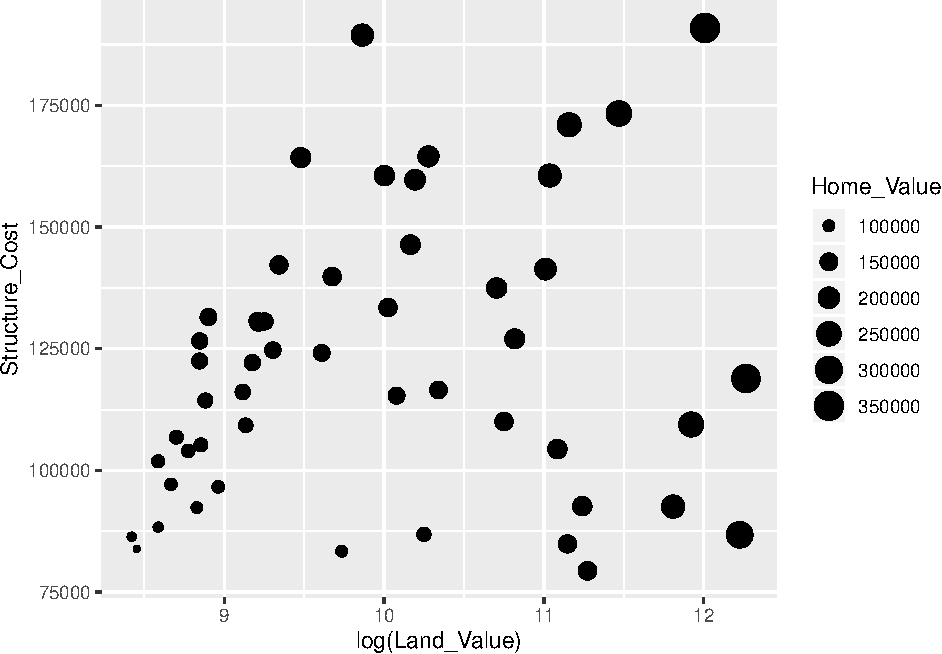
\includegraphics{R/Rgraphics/figures/unnamed-chunk-149-1.pdf}

\begin{enumerate}
\def\labelenumi{\arabic{enumi}.}
\setcounter{enumi}{1}
\tightlist
\item
  Constants are \textbf{fixed} to aesthetics outside the \texttt{aes()}
  call
\end{enumerate}

\begin{Shaded}
\begin{Highlighting}[]
\NormalTok{p1 }\OperatorTok{+}
\StringTok{  }\KeywordTok{geom_point}\NormalTok{(}\DataTypeTok{size =} \DecValTok{2}\NormalTok{)}
\end{Highlighting}
\end{Shaded}

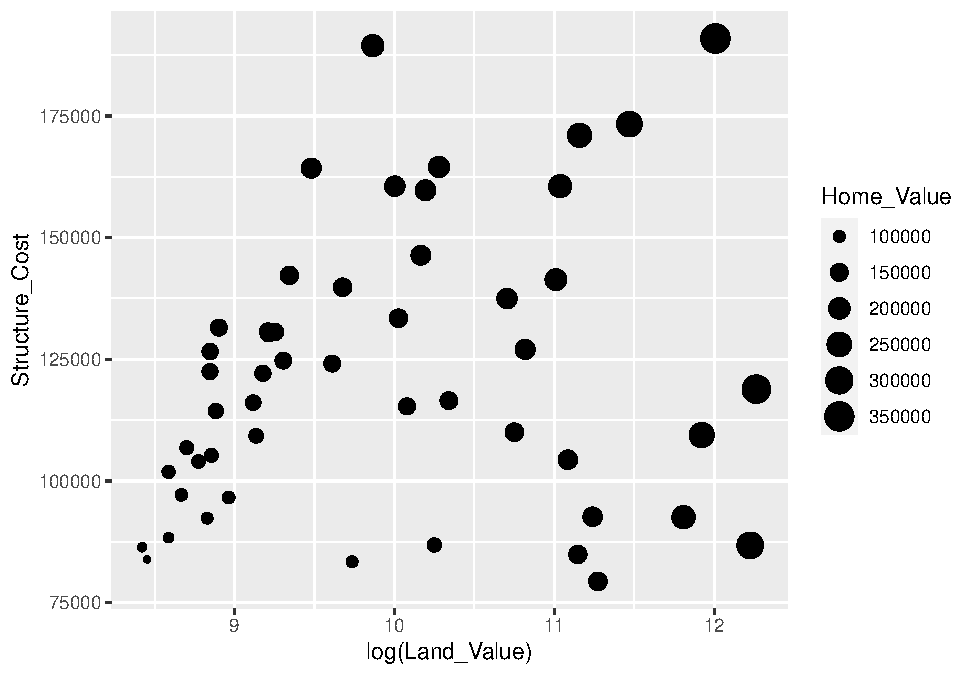
\includegraphics{R/Rgraphics/figures/unnamed-chunk-150-1.pdf}

This sometimes leads to confusion, as in this example:

\begin{Shaded}
\begin{Highlighting}[]
\NormalTok{p1 }\OperatorTok{+}
\StringTok{  }\KeywordTok{geom_point}\NormalTok{(}\KeywordTok{aes}\NormalTok{(}\DataTypeTok{size =} \DecValTok{2}\NormalTok{),}\CommentTok{# incorrect! 2 is not a variable}
             \DataTypeTok{color=}\StringTok{"red"}\NormalTok{) }\CommentTok{# this is fine -- all points red}
\end{Highlighting}
\end{Shaded}

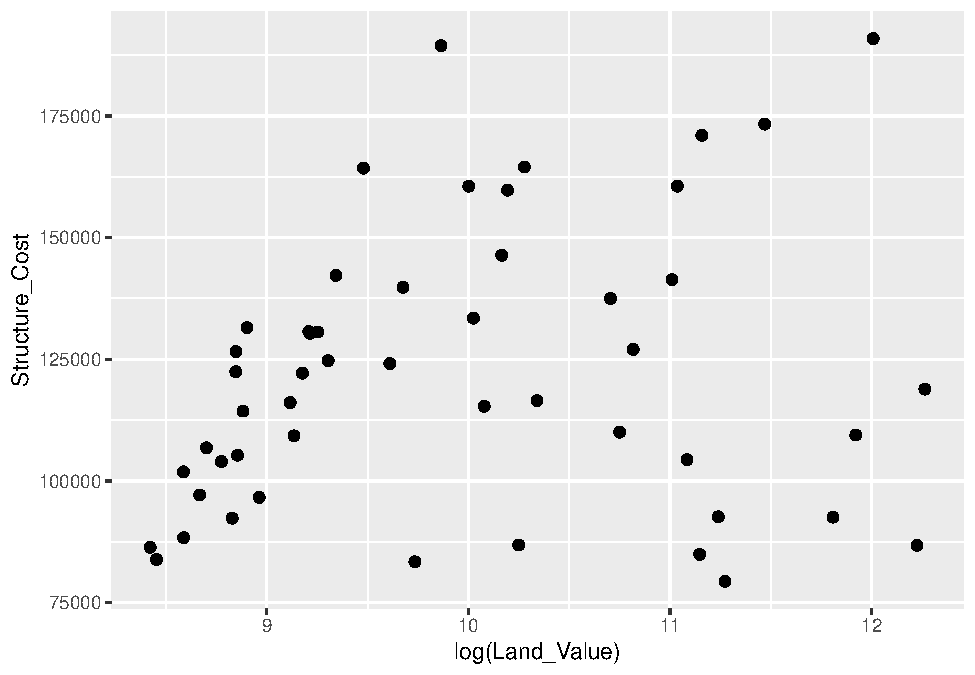
\includegraphics{R/Rgraphics/figures/unnamed-chunk-151-1.pdf}

\subsection{Mapping variables to other
aesthetics}\label{mapping-variables-to-other-aesthetics}

Other aesthetics are mapped in the same way as x and y in the previous
example.

\begin{Shaded}
\begin{Highlighting}[]
\NormalTok{p1 }\OperatorTok{+}
\StringTok{  }\KeywordTok{geom_point}\NormalTok{(}\KeywordTok{aes}\NormalTok{(}\DataTypeTok{color =}\NormalTok{ Home_Value, }\DataTypeTok{shape =}\NormalTok{ region))}
\end{Highlighting}
\end{Shaded}

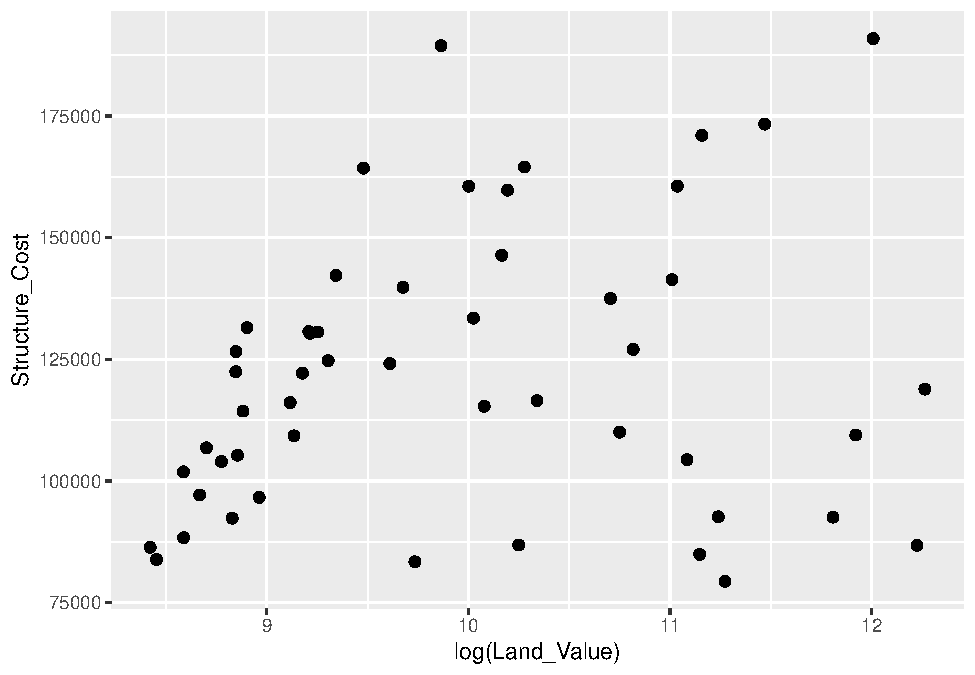
\includegraphics{R/Rgraphics/figures/unnamed-chunk-152-1.pdf}

\subsection{Exercise 0}\label{exercise-0-2}

The data for the exercises is available in the
\texttt{dataSets/EconomistData.csv} file. Read it in with

\begin{Shaded}
\begin{Highlighting}[]
\NormalTok{dat <-}\StringTok{ }\KeywordTok{read_csv}\NormalTok{(}\StringTok{"dataSets/EconomistData.csv"}\NormalTok{)}
\end{Highlighting}
\end{Shaded}

Original sources for these data are
\url{http://www.transparency.org/content/download/64476/1031428}
\url{http://hdrstats.undp.org/en/indicators/display_cf_xls_indicator.cfm?indicator_id=103106\&lang=en}

These data consist of \emph{Human Development Index} and
\emph{Corruption Perception Index} scores for several countries.

\begin{enumerate}
\def\labelenumi{\arabic{enumi}.}
\tightlist
\item
  Create a scatter plot with \texttt{CPI} on the x axis and \texttt{HDI}
  on the y axis.
\end{enumerate}

\begin{Shaded}
\begin{Highlighting}[]
\NormalTok{## }
\end{Highlighting}
\end{Shaded}

\begin{enumerate}
\def\labelenumi{\arabic{enumi}.}
\setcounter{enumi}{1}
\tightlist
\item
  Color the points in the previous plot blue.
\end{enumerate}

\begin{Shaded}
\begin{Highlighting}[]
\NormalTok{## }
\end{Highlighting}
\end{Shaded}

\begin{enumerate}
\def\labelenumi{\arabic{enumi}.}
\setcounter{enumi}{2}
\tightlist
\item
  Map the color of the the points to \texttt{Region}.
\end{enumerate}

\begin{Shaded}
\begin{Highlighting}[]
\NormalTok{## }
\end{Highlighting}
\end{Shaded}

\begin{enumerate}
\def\labelenumi{\arabic{enumi}.}
\setcounter{enumi}{3}
\tightlist
\item
  Keeping color mapped to \texttt{Region}, make the points bigger by
  setting size to 2
\end{enumerate}

\begin{Shaded}
\begin{Highlighting}[]
\NormalTok{## }
\end{Highlighting}
\end{Shaded}

\begin{enumerate}
\def\labelenumi{\arabic{enumi}.}
\setcounter{enumi}{4}
\tightlist
\item
  Keeping color mapped to \texttt{Region}, map the size of the points to
  \texttt{HDI\_Rank}
\end{enumerate}

\begin{Shaded}
\begin{Highlighting}[]
\NormalTok{## }
\end{Highlighting}
\end{Shaded}

\section{Statistical transformations}\label{statistical-transformations}

\subsection{Why transform data?}\label{why-transform-data}

Some plot types (such as scatterplots) do not require transformations;
each point is plotted at x and y coordinates equal to the original
value. Other plots, such as boxplots, histograms, prediction lines etc.
require statistical transformations:

\begin{itemize}
\tightlist
\item
  for a boxplot the y values must be transformed to the median and
  1.5(IQR)
\item
  for a smoother the y values must be transformed into predicted values
\end{itemize}

Each geom has a default statistic, but these can be changed. For
example, the default statistic for \texttt{geom\_histogram()} is
\texttt{stat\_bin()}:

\begin{Shaded}
\begin{Highlighting}[]
\KeywordTok{args}\NormalTok{(geom_histogram)}
\end{Highlighting}
\end{Shaded}

\begin{verbatim}
## function (mapping = NULL, data = NULL, stat = "bin", position = "stack", 
##     ..., binwidth = NULL, bins = NULL, na.rm = FALSE, show.legend = NA, 
##     inherit.aes = TRUE) 
## NULL
\end{verbatim}

\begin{Shaded}
\begin{Highlighting}[]
\KeywordTok{args}\NormalTok{(stat_bin)}
\end{Highlighting}
\end{Shaded}

\begin{verbatim}
## function (mapping = NULL, data = NULL, geom = "bar", position = "stack", 
##     ..., binwidth = NULL, bins = NULL, center = NULL, boundary = NULL, 
##     breaks = NULL, closed = c("right", "left"), pad = FALSE, 
##     na.rm = FALSE, show.legend = NA, inherit.aes = TRUE) 
## NULL
\end{verbatim}

Here is a list of geoms and their default statistics
\url{https://ggplot2.tidyverse.org/reference/}

\subsection{Setting arguments}\label{setting-arguments}

Arguments to \texttt{stat\_} functions can be passed through
\texttt{geom\_} functions. This can be slightly annoying because in
order to change it you have to first determine which stat the geom uses,
then determine the arguments to that stat.

For example, here is the default histogram of \texttt{Home\_Value}:

\begin{Shaded}
\begin{Highlighting}[]
\NormalTok{p2 <-}\StringTok{ }\KeywordTok{ggplot}\NormalTok{(housing, }\KeywordTok{aes}\NormalTok{(}\DataTypeTok{x =}\NormalTok{ Home_Value))}
\NormalTok{p2 }\OperatorTok{+}\StringTok{ }\KeywordTok{geom_histogram}\NormalTok{()}
\end{Highlighting}
\end{Shaded}

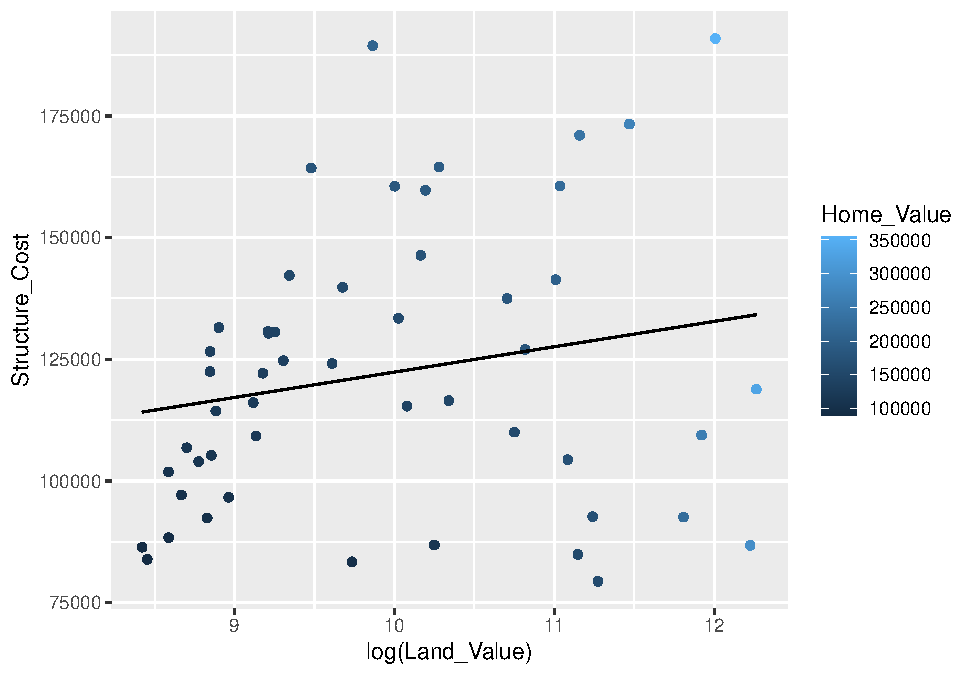
\includegraphics{R/Rgraphics/figures/unnamed-chunk-160-1.pdf}

can change it by passing the \texttt{binwidth} argument to the
\texttt{stat\_bin()} function:

\begin{Shaded}
\begin{Highlighting}[]
\NormalTok{p2 }\OperatorTok{+}\StringTok{ }\KeywordTok{geom_histogram}\NormalTok{(}\DataTypeTok{stat =} \StringTok{"bin"}\NormalTok{, }\DataTypeTok{binwidth=}\DecValTok{4000}\NormalTok{)}
\end{Highlighting}
\end{Shaded}

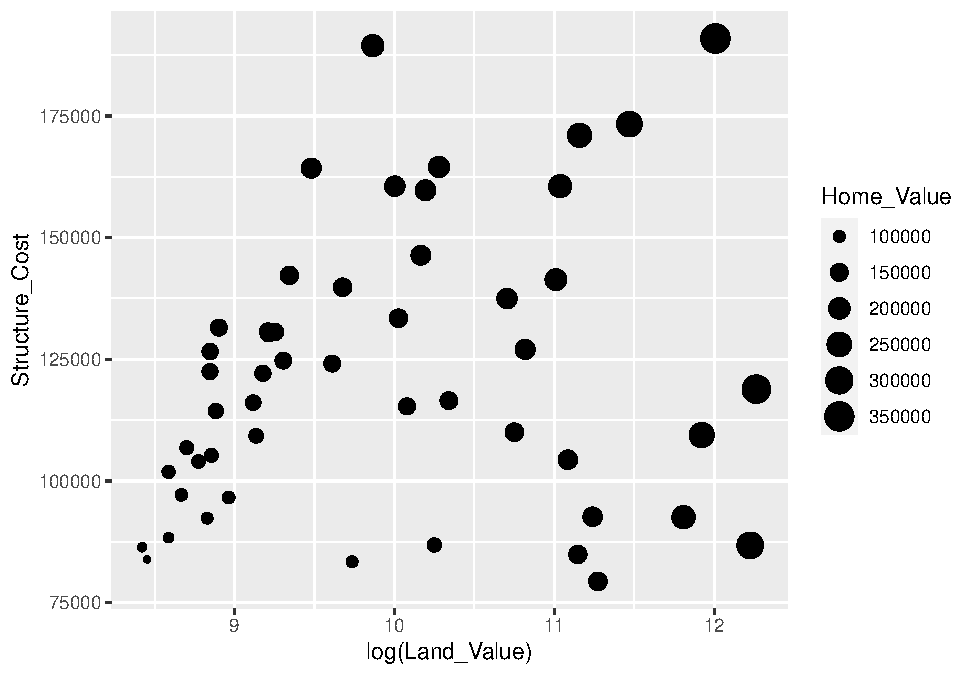
\includegraphics{R/Rgraphics/figures/unnamed-chunk-161-1.pdf}

\subsection{Changing the
transformation}\label{changing-the-transformation}

Sometimes the default statistical transformation is not what you need.
This is often the case with pre-summarized data:

\begin{Shaded}
\begin{Highlighting}[]
\NormalTok{housing_sum <-}\StringTok{ }
\StringTok{  }\NormalTok{housing }\OperatorTok
\StringTok{  }\KeywordTok{group_by}\NormalTok{(State) }\OperatorTok
\StringTok{  }\KeywordTok{summarize}\NormalTok{(}\DataTypeTok{Home_Value_Mean =} \KeywordTok{mean}\NormalTok{(Home_Value)) }\OperatorTok
\StringTok{  }\KeywordTok{ungroup}\NormalTok{()}

\KeywordTok{head}\NormalTok{(housing_sum)}
\end{Highlighting}
\end{Shaded}

\begin{verbatim}
## # A tibble: 6 x 2
##   State Home_Value_Mean
##   <chr>           <dbl>
## 1 AK            147385.
## 2 AL             92545.
## 3 AR             82077.
## 4 AZ            140756.
## 5 CA            282808.
## 6 CO            158176.
\end{verbatim}

\begin{Shaded}
\begin{Highlighting}[]
\KeywordTok{ggplot}\NormalTok{(housing_sum, }\KeywordTok{aes}\NormalTok{(}\DataTypeTok{x=}\NormalTok{State, }\DataTypeTok{y=}\NormalTok{Home_Value_Mean)) }\OperatorTok{+}\StringTok{ }
\StringTok{  }\KeywordTok{geom_bar}\NormalTok{()}
\end{Highlighting}
\end{Shaded}

\begin{verbatim}
## Error: stat_count() must not be used with a y aesthetic.
\end{verbatim}

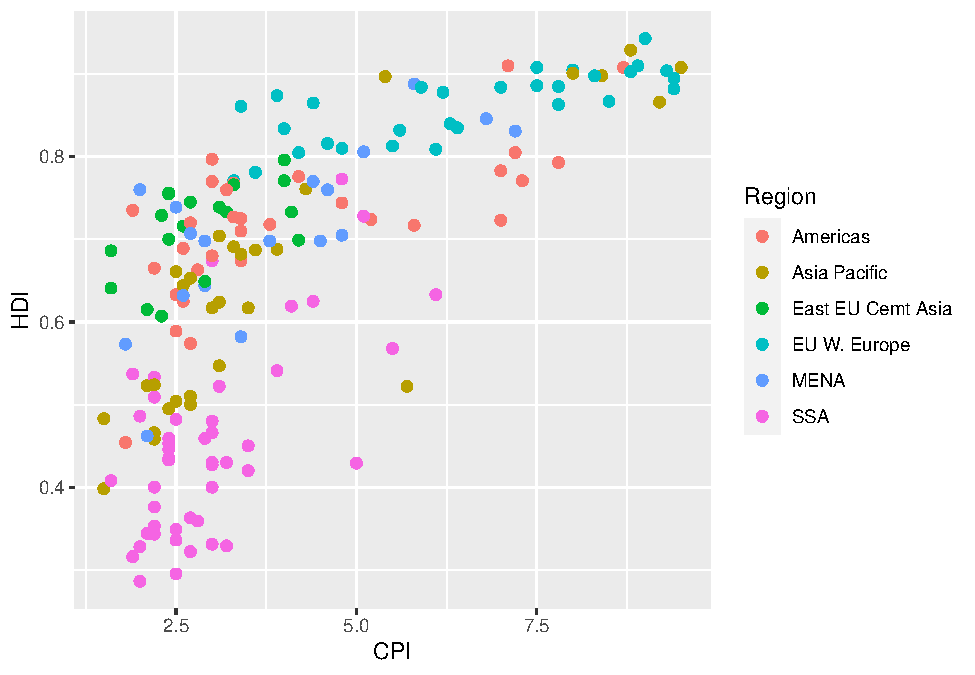
\includegraphics{R/Rgraphics/figures/unnamed-chunk-163-1.pdf}

What is the problem with the previous plot? Basically we take binned and
summarized data and ask ggplot to bin and summarize it again (remember,
\texttt{geom\_bar()} defaults to \texttt{stat\ =\ stat\_count};
obviously this will not work. We can fix it by telling
\texttt{geom\_bar()} to use a different statistical transformation
function:

\begin{Shaded}
\begin{Highlighting}[]
\KeywordTok{ggplot}\NormalTok{(housing_sum, }\KeywordTok{aes}\NormalTok{(}\DataTypeTok{x=}\NormalTok{State, }\DataTypeTok{y=}\NormalTok{Home_Value_Mean)) }\OperatorTok{+}\StringTok{ }
\StringTok{  }\KeywordTok{geom_bar}\NormalTok{(}\DataTypeTok{stat=}\StringTok{"identity"}\NormalTok{)}
\end{Highlighting}
\end{Shaded}

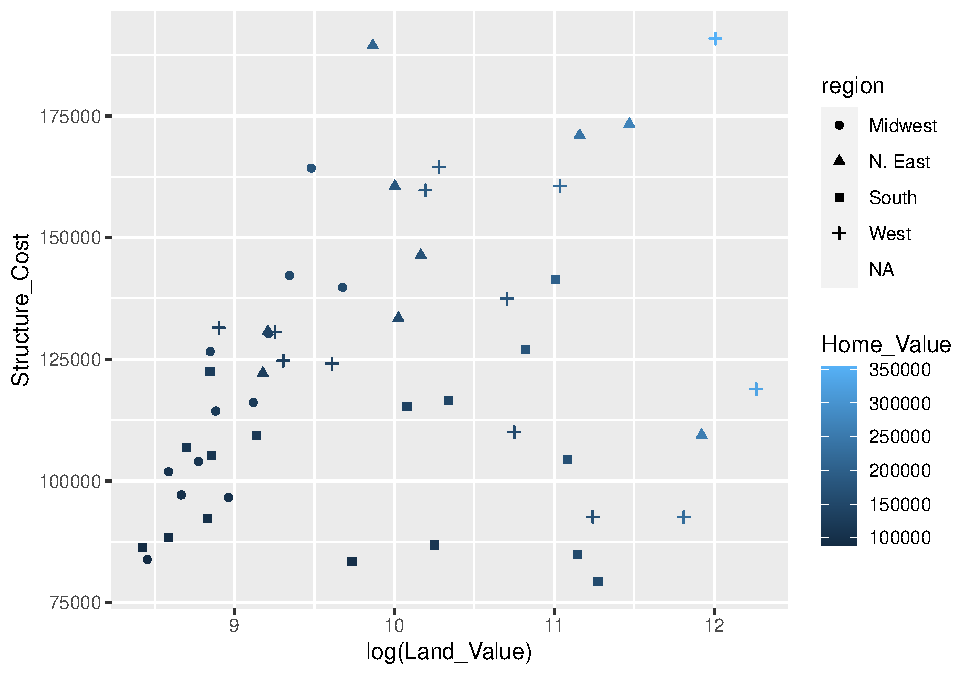
\includegraphics{R/Rgraphics/figures/unnamed-chunk-164-1.pdf}

\subsection{Exercise 1}\label{exercise-1-2}

\begin{enumerate}
\def\labelenumi{\arabic{enumi}.}
\tightlist
\item
  Re-create a scatter plot with \texttt{CPI} on the x axis and
  \texttt{HDI} on the y axis (as you did in the previous exercise).
\end{enumerate}

\begin{Shaded}
\begin{Highlighting}[]
\NormalTok{## }
\end{Highlighting}
\end{Shaded}

\begin{enumerate}
\def\labelenumi{\arabic{enumi}.}
\setcounter{enumi}{1}
\tightlist
\item
  Overlay a smoothing line on top of the scatter plot using
  \texttt{geom\_smooth()}.
\end{enumerate}

\begin{Shaded}
\begin{Highlighting}[]
\NormalTok{## }
\end{Highlighting}
\end{Shaded}

\begin{enumerate}
\def\labelenumi{\arabic{enumi}.}
\setcounter{enumi}{2}
\tightlist
\item
  Make the smoothing line in \texttt{geom\_smooth()} less smooth. Hint:
  see \texttt{?loess}.
\end{enumerate}

\begin{Shaded}
\begin{Highlighting}[]
\NormalTok{## }
\end{Highlighting}
\end{Shaded}

\begin{enumerate}
\def\labelenumi{\arabic{enumi}.}
\setcounter{enumi}{3}
\tightlist
\item
  Change the smoothing line in \texttt{geom\_smooth()} to use a linear
  model for the predictions. Hint: see \texttt{?stat\_smooth}.
\end{enumerate}

\begin{Shaded}
\begin{Highlighting}[]
\NormalTok{## }
\end{Highlighting}
\end{Shaded}

\begin{enumerate}
\def\labelenumi{\arabic{enumi}.}
\setcounter{enumi}{4}
\tightlist
\item
  BONUS: Overlay a loess \texttt{(method\ =\ "loess")} smoothing line on
  top of the scatter plot using \texttt{geom\_line()}. Hint: change the
  statistical transformation.
\end{enumerate}

\begin{Shaded}
\begin{Highlighting}[]
\NormalTok{## }
\end{Highlighting}
\end{Shaded}

\section{Scales}\label{scales}

\subsection{Controlling aesthetic
mapping}\label{controlling-aesthetic-mapping}

Aesthetic mapping (i.e., with \texttt{aes()}) only says that a variable
should be mapped to an aesthetic. It doesn't say \emph{how} that should
happen. For example, when mapping a variable to \emph{shape} with
\texttt{aes(shape\ =\ x)} you don't say \emph{what} shapes should be
used. Similarly, \texttt{aes(color\ =\ y)} doesn't say \emph{what}
colors should be used. Also, \texttt{aes(size\ =\ z)} doesn't say
\emph{what} sizes should be used. Describing what colors/shapes/sizes
etc. to use is done by modifying the corresponding \emph{scale}. In
\texttt{ggplot2} scales include

\begin{itemize}
\tightlist
\item
  position
\item
  color and fill
\item
  size
\item
  shape
\item
  line type
\end{itemize}

Scales are modified with a series of functions using a
\texttt{scale\_\textless{}aesthetic\textgreater{}\_\textless{}type\textgreater{}}
naming scheme. Try typing \texttt{scale\_\textless{}tab\textgreater{}}
to see a list of scale modification functions.

\subsection{Common scale arguments}\label{common-scale-arguments}

The following arguments are common to most scales in \texttt{ggplot2}:

\begin{itemize}
\tightlist
\item
  \textbf{name:} the axis or legend title
\item
  \textbf{limits:} the minimum and maximum of the scale
\item
  \textbf{breaks:} the points along the scale where labels should appear
\item
  \textbf{labels:} the labels that appear at each break
\end{itemize}

Specific scale functions may have additional arguments; for example, the
\texttt{scale\_color\_continuous()} function has arguments \texttt{low}
and \texttt{high} for setting the colors at the low and high end of the
scale.

\subsection{Scale modification
examples}\label{scale-modification-examples}

Start by constructing a dotplot showing the distribution of home values
by \texttt{Date} and \texttt{State}.

\begin{Shaded}
\begin{Highlighting}[]
\NormalTok{p4 <-}\StringTok{ }\KeywordTok{ggplot}\NormalTok{(housing, }\KeywordTok{aes}\NormalTok{(}\DataTypeTok{x =}\NormalTok{ State, }\DataTypeTok{y =}\NormalTok{ Home_Price_Index)) }\OperatorTok{+}\StringTok{ }
\StringTok{    }\KeywordTok{geom_point}\NormalTok{(}\KeywordTok{aes}\NormalTok{(}\DataTypeTok{color =}\NormalTok{ Date), }\DataTypeTok{alpha =} \FloatTok{0.5}\NormalTok{, }\DataTypeTok{size =} \FloatTok{1.5}\NormalTok{,}
               \DataTypeTok{position =} \KeywordTok{position_jitter}\NormalTok{(}\DataTypeTok{width =} \FloatTok{0.25}\NormalTok{, }\DataTypeTok{height =} \DecValTok{0}\NormalTok{))}
\end{Highlighting}
\end{Shaded}

Now modify the breaks for the color scales

\begin{Shaded}
\begin{Highlighting}[]
\NormalTok{p4 }\OperatorTok{+}\StringTok{ }
\StringTok{  }\KeywordTok{scale_color_continuous}\NormalTok{(}\DataTypeTok{name=}\StringTok{""}\NormalTok{,}
                         \DataTypeTok{breaks =} \KeywordTok{c}\NormalTok{(}\DecValTok{1976}\NormalTok{, }\DecValTok{1994}\NormalTok{, }\DecValTok{2013}\NormalTok{),}
                         \DataTypeTok{labels =} \KeywordTok{c}\NormalTok{(}\StringTok{"'76"}\NormalTok{, }\StringTok{"'94"}\NormalTok{, }\StringTok{"'13"}\NormalTok{))}
\end{Highlighting}
\end{Shaded}

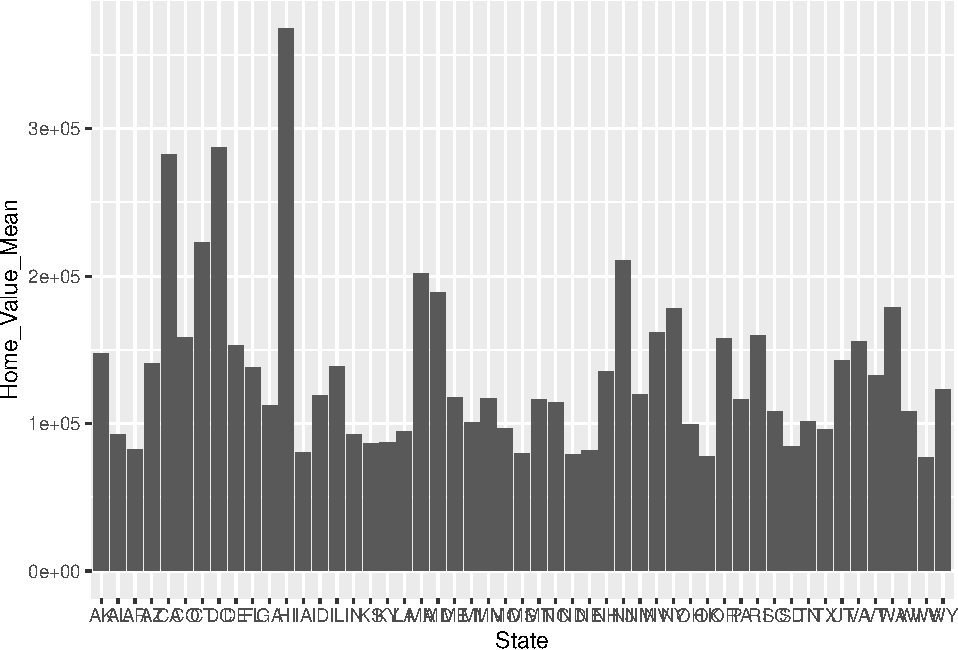
\includegraphics{R/Rgraphics/figures/unnamed-chunk-171-1.pdf}

Next change the low and high values to blue and red:

\begin{Shaded}
\begin{Highlighting}[]
\NormalTok{p4 }\OperatorTok{+}
\StringTok{  }\KeywordTok{scale_color_continuous}\NormalTok{(}\DataTypeTok{name=}\StringTok{""}\NormalTok{,}
                         \DataTypeTok{breaks =} \KeywordTok{c}\NormalTok{(}\DecValTok{1976}\NormalTok{, }\DecValTok{1994}\NormalTok{, }\DecValTok{2013}\NormalTok{),}
                         \DataTypeTok{labels =} \KeywordTok{c}\NormalTok{(}\StringTok{"'76"}\NormalTok{, }\StringTok{"'94"}\NormalTok{, }\StringTok{"'13"}\NormalTok{),}
                         \DataTypeTok{low =} \StringTok{"blue"}\NormalTok{, }\DataTypeTok{high =} \StringTok{"red"}\NormalTok{)}
\end{Highlighting}
\end{Shaded}

\includegraphics{R/Rgraphics/figures/unnamed-chunk-172-1.pdf}

\subsection{Using different color
scales}\label{using-different-color-scales}

\texttt{ggplot2} has a wide variety of color scales; here is an example
using \texttt{scale\_color\_gradient2()} to interpolate between three
different colors.

\begin{Shaded}
\begin{Highlighting}[]
\NormalTok{p4 }\OperatorTok{+}
\StringTok{  }\KeywordTok{scale_color_gradient2}\NormalTok{(}\DataTypeTok{name=}\StringTok{""}\NormalTok{,}
                        \DataTypeTok{breaks =} \KeywordTok{c}\NormalTok{(}\DecValTok{1976}\NormalTok{, }\DecValTok{1994}\NormalTok{, }\DecValTok{2013}\NormalTok{),}
                        \DataTypeTok{labels =} \KeywordTok{c}\NormalTok{(}\StringTok{"'76"}\NormalTok{, }\StringTok{"'94"}\NormalTok{, }\StringTok{"'13"}\NormalTok{),}
                        \DataTypeTok{low =} \StringTok{"blue"}\NormalTok{,}
                        \DataTypeTok{high =} \StringTok{"red"}\NormalTok{,}
                        \DataTypeTok{mid =} \StringTok{"gray60"}\NormalTok{,}
                        \DataTypeTok{midpoint =} \DecValTok{1994}\NormalTok{)}
\end{Highlighting}
\end{Shaded}

\includegraphics{R/Rgraphics/figures/unnamed-chunk-173-1.pdf}

\subsection{Available scales}\label{available-scales}

\begin{itemize}
\tightlist
\item
  Partial combination matrix of available scales
\end{itemize}

\begin{longtable}[]{@{}lll@{}}
\toprule
\texttt{scale\_} & Types & Examples\tabularnewline
\midrule
\endhead
\texttt{scale\_color\_} & \texttt{identity} &
\texttt{scale\_fill\_continuous()}\tabularnewline
\texttt{scale\_fill\_} & \texttt{manual} &
\texttt{scale\_color\_discrete()}\tabularnewline
\texttt{scale\_size\_} & \texttt{continuous} &
\texttt{scale\_size\_manual()}\tabularnewline
& \texttt{discrete} & \texttt{scale\_size\_discrete()}\tabularnewline
& &\tabularnewline
\texttt{scale\_shape\_} & \texttt{discrete} &
\texttt{scale\_shape\_discrete()}\tabularnewline
\texttt{scale\_linetype\_} & \texttt{identity} &
\texttt{scale\_shape\_manual()}\tabularnewline
& \texttt{manual} & \texttt{scale\_linetype\_discrete()}\tabularnewline
& &\tabularnewline
\texttt{scale\_x\_} & \texttt{continuous} &
\texttt{scale\_x\_continuous()}\tabularnewline
\texttt{scale\_y\_} & \texttt{discrete} &
\texttt{scale\_y\_discrete()}\tabularnewline
& \texttt{reverse} & \texttt{scale\_x\_log()}\tabularnewline
& \texttt{log} & \texttt{scale\_y\_reverse()}\tabularnewline
& \texttt{date} & \texttt{scale\_x\_date()}\tabularnewline
& \texttt{datetime} & \texttt{scale\_y\_datetime()}\tabularnewline
\bottomrule
\end{longtable}

Note that in RStudio you can type \texttt{scale\_} followed by
\texttt{tab} to get the whole list of available scales. For a complete
list of available scales see
\url{https://ggplot2.tidyverse.org/reference/}

\subsection{Exercise 2}\label{exercise-2-1}

\begin{enumerate}
\def\labelenumi{\arabic{enumi}.}
\tightlist
\item
  Create a scatter plot with \texttt{CPI} on the x axis and \texttt{HDI}
  on the y axis. Color the points to indicate \texttt{Region}.
\end{enumerate}

\begin{Shaded}
\begin{Highlighting}[]
\NormalTok{## }
\end{Highlighting}
\end{Shaded}

\begin{enumerate}
\def\labelenumi{\arabic{enumi}.}
\setcounter{enumi}{1}
\tightlist
\item
  Modify the x, y, and color scales so that they have more
  easily-understood names (e.g., spell out ``Human development Index''
  instead of \texttt{HDI}). Hint: see \texttt{?scale\_x\_continous},
  \texttt{?scale\_y\_continuous}, and \texttt{?scale\_color\_discrete}.
\end{enumerate}

\begin{Shaded}
\begin{Highlighting}[]
\NormalTok{## }
\end{Highlighting}
\end{Shaded}

\begin{enumerate}
\def\labelenumi{\arabic{enumi}.}
\setcounter{enumi}{2}
\tightlist
\item
  Modify the color scale to use specific values of your choosing. Hint:
  see \texttt{?scale\_color\_manual}. NOTE: you can specify color by
  name (e.g., ``blue'') or by ``Hex value'' --- see
  \url{https://www.color-hex.com/}.
\end{enumerate}

\begin{Shaded}
\begin{Highlighting}[]
\NormalTok{## }
\end{Highlighting}
\end{Shaded}

\section{Faceting}\label{faceting}

\subsection{What is faceting?}\label{what-is-faceting}

\begin{itemize}
\tightlist
\item
  Faceting is \texttt{ggplot2} parlance for \textbf{small multiples}
\item
  The idea is to create separate graphs for subsets of data
\item
  \texttt{ggplot2} offers two functions for creating small multiples:

  \begin{enumerate}
  \def\labelenumi{\arabic{enumi}.}
  \tightlist
  \item
    \texttt{facet\_wrap()}: define subsets as the levels of a single
    grouping variable
  \item
    \texttt{facet\_grid()}: define subsets as the crossing of two
    grouping variables
  \end{enumerate}
\item
  Facilitates comparison among plots, not just of geoms within a plot
\end{itemize}

\subsection{What is the trend in housing prices in each
state?}\label{what-is-the-trend-in-housing-prices-in-each-state}

\begin{itemize}
\tightlist
\item
  Start by using a technique we already know; map \texttt{State} to
  color:
\end{itemize}

\begin{Shaded}
\begin{Highlighting}[]
\NormalTok{p5 <-}\StringTok{ }\KeywordTok{ggplot}\NormalTok{(housing, }\KeywordTok{aes}\NormalTok{(}\DataTypeTok{x =}\NormalTok{ Date, }\DataTypeTok{y =}\NormalTok{ Home_Value))}
\NormalTok{p5 }\OperatorTok{+}\StringTok{ }\KeywordTok{geom_line}\NormalTok{(}\KeywordTok{aes}\NormalTok{(}\DataTypeTok{color =}\NormalTok{ State))  }
\end{Highlighting}
\end{Shaded}

\includegraphics{R/Rgraphics/figures/unnamed-chunk-177-1.pdf}

There are two problems here; there are too many states to distinguish
each one by color, and the lines obscure one another.

\subsection{Faceting to the rescue}\label{faceting-to-the-rescue}

We can remedy the deficiencies of the previous plot by faceting by
\texttt{State} rather than mapping \texttt{State} to color.

\begin{Shaded}
\begin{Highlighting}[]
\NormalTok{p5 <-}\StringTok{ }\NormalTok{p5 }\OperatorTok{+}\StringTok{ }\KeywordTok{geom_line}\NormalTok{() }\OperatorTok{+}
\StringTok{   }\KeywordTok{facet_wrap}\NormalTok{(}\OperatorTok{~}\StringTok{ }\NormalTok{State, }\DataTypeTok{ncol =} \DecValTok{10}\NormalTok{)}
\NormalTok{p5}
\end{Highlighting}
\end{Shaded}

\includegraphics{R/Rgraphics/figures/unnamed-chunk-178-1.pdf}

\section{Themes}\label{themes}

\subsection{What are themes?}\label{what-are-themes}

The \texttt{ggplot2} theme system handles non-data plot elements such
as:

\begin{itemize}
\tightlist
\item
  Axis label properties (e.g., font, size, color, etc.)
\item
  Plot background
\item
  Facet label background
\item
  Legend appearance
\end{itemize}

Built-in themes include:

\begin{itemize}
\tightlist
\item
  \texttt{theme\_gray()} (default)
\item
  \texttt{theme\_bw()}
\item
  \texttt{theme\_classic()}
\end{itemize}

\begin{Shaded}
\begin{Highlighting}[]
\NormalTok{p5 }\OperatorTok{+}\StringTok{ }\KeywordTok{theme_linedraw}\NormalTok{()}
\end{Highlighting}
\end{Shaded}

\includegraphics{R/Rgraphics/figures/unnamed-chunk-179-1.pdf}

\begin{Shaded}
\begin{Highlighting}[]
\NormalTok{p5 }\OperatorTok{+}\StringTok{ }\KeywordTok{theme_light}\NormalTok{()}
\end{Highlighting}
\end{Shaded}

\includegraphics{R/Rgraphics/figures/unnamed-chunk-180-1.pdf} You can
see a list of available built-in themes here
\url{https://ggplot2.tidyverse.org/reference/}

\subsection{Overriding theme defaults}\label{overriding-theme-defaults}

Specific theme elements can be overridden using \texttt{theme()}. For
example:

\begin{Shaded}
\begin{Highlighting}[]
\CommentTok{# theme(thing_to_modify = modifying_function(arg1, arg2))}

\NormalTok{p5 }\OperatorTok{+}\StringTok{ }\KeywordTok{theme_minimal}\NormalTok{() }\OperatorTok{+}
\StringTok{  }\KeywordTok{theme}\NormalTok{(}\DataTypeTok{text =} \KeywordTok{element_text}\NormalTok{(}\DataTypeTok{color =} \StringTok{"turquoise"}\NormalTok{))  }
\end{Highlighting}
\end{Shaded}

\includegraphics{R/Rgraphics/figures/unnamed-chunk-181-1.pdf}

All theme options are documented in \texttt{?theme}. We can also see the
existing default values using:

\begin{Shaded}
\begin{Highlighting}[]
\KeywordTok{theme_get}\NormalTok{()}
\end{Highlighting}
\end{Shaded}

\subsection{Creating \& saving new
themes}\label{creating-saving-new-themes}

You can create new themes, as in the following example:

\begin{Shaded}
\begin{Highlighting}[]
\NormalTok{theme_new <-}\StringTok{ }\KeywordTok{theme_bw}\NormalTok{() }\OperatorTok{+}
\StringTok{  }\KeywordTok{theme}\NormalTok{(}\DataTypeTok{plot.background =} \KeywordTok{element_rect}\NormalTok{(}\DataTypeTok{size =} \DecValTok{1}\NormalTok{, }\DataTypeTok{color =} \StringTok{"blue"}\NormalTok{, }\DataTypeTok{fill =} \StringTok{"black"}\NormalTok{),}
        \DataTypeTok{text =} \KeywordTok{element_text}\NormalTok{(}\DataTypeTok{size =} \DecValTok{12}\NormalTok{, }\DataTypeTok{color =} \StringTok{"ivory"}\NormalTok{),}
        \DataTypeTok{axis.text.y =} \KeywordTok{element_text}\NormalTok{(}\DataTypeTok{colour =} \StringTok{"purple"}\NormalTok{),}
        \DataTypeTok{axis.text.x =} \KeywordTok{element_text}\NormalTok{(}\DataTypeTok{colour =} \StringTok{"red"}\NormalTok{),}
        \DataTypeTok{panel.background =} \KeywordTok{element_rect}\NormalTok{(}\DataTypeTok{fill =} \StringTok{"pink"}\NormalTok{),}
        \DataTypeTok{strip.background =} \KeywordTok{element_rect}\NormalTok{(}\DataTypeTok{fill =} \KeywordTok{muted}\NormalTok{(}\StringTok{"orange"}\NormalTok{)))}

\NormalTok{p5 }\OperatorTok{+}\StringTok{ }\NormalTok{theme_new}
\end{Highlighting}
\end{Shaded}

\includegraphics{R/Rgraphics/figures/unnamed-chunk-183-1.pdf}

\section{Saving plots}\label{saving-plots}

We can save a plot to either a vector (e.g., pdf, eps, ps, svg) or
raster (e.g., jpg, png, tiff, bmp, wmf) graphics file using the
\texttt{ggsave()} function:

\begin{Shaded}
\begin{Highlighting}[]
\KeywordTok{ggsave}\NormalTok{(}\DataTypeTok{filename =} \StringTok{"myplot.pdf"}\NormalTok{, }\DataTypeTok{plot =}\NormalTok{ p5, }\DataTypeTok{device =} \StringTok{"pdf"}\NormalTok{, }\DataTypeTok{height =} \DecValTok{6}\NormalTok{, }\DataTypeTok{width =} \DecValTok{6}\NormalTok{, }\DataTypeTok{units =} \StringTok{"in"}\NormalTok{)}
\end{Highlighting}
\end{Shaded}

\section{The \#1 FAQ}\label{the-1-faq}

\subsection{Map aesthetic to different
columns}\label{map-aesthetic-to-different-columns}

The most frequently asked question goes something like this: \emph{I
have two variables in my data.frame, and I'd like to plot them as
separate points, with different color depending on which variable it is.
How do I do that?}

\textbf{Wrong}

Fixing, rather than mapping, the color aesthetic:

\begin{enumerate}
\def\labelenumi{\arabic{enumi}.}
\tightlist
\item
  Produces verbose code when using many colors
\item
  Results in no legend being produced
\item
  Means you cannot change color scales
\end{enumerate}

\begin{Shaded}
\begin{Highlighting}[]
\NormalTok{housing_byyear <-}\StringTok{ }
\StringTok{  }\NormalTok{housing }\OperatorTok
\StringTok{  }\KeywordTok{group_by}\NormalTok{(Date) }\OperatorTok
\StringTok{  }\KeywordTok{summarize}\NormalTok{(}\DataTypeTok{Home_Value_Mean =} \KeywordTok{mean}\NormalTok{(Home_Value),}
            \DataTypeTok{Land_Value_Mean =} \KeywordTok{mean}\NormalTok{(Land_Value)) }\OperatorTok
\StringTok{  }\KeywordTok{ungroup}\NormalTok{()}

\KeywordTok{ggplot}\NormalTok{(housing_byyear, }\KeywordTok{aes}\NormalTok{(}\DataTypeTok{x=}\NormalTok{Date)) }\OperatorTok{+}
\StringTok{  }\KeywordTok{geom_line}\NormalTok{(}\KeywordTok{aes}\NormalTok{(}\DataTypeTok{y=}\NormalTok{Home_Value_Mean), }\DataTypeTok{color=}\StringTok{"red"}\NormalTok{) }\OperatorTok{+}
\StringTok{  }\KeywordTok{geom_line}\NormalTok{(}\KeywordTok{aes}\NormalTok{(}\DataTypeTok{y=}\NormalTok{Land_Value_Mean), }\DataTypeTok{color=}\StringTok{"blue"}\NormalTok{)}
\end{Highlighting}
\end{Shaded}

\includegraphics{R/Rgraphics/figures/unnamed-chunk-185-1.pdf}

\textbf{Right}

To avoid these pitfalls, we need to \textbf{map} our data to the color
aesthetic. We can do this by \textbf{reshaping} our data from
\textbf{wide format} to \textbf{long format}. Here is the logic behind
this process:

\includegraphics{R/Rgraphics/images/wide_vs_long.png}

Here's the code that implements this transformation:

\begin{Shaded}
\begin{Highlighting}[]
\NormalTok{home_land_byyear <-}\StringTok{ }\KeywordTok{gather}\NormalTok{(housing_byyear,}
                           \DataTypeTok{value =} \StringTok{"value"}\NormalTok{,}
                           \DataTypeTok{key =} \StringTok{"type"}\NormalTok{,}
\NormalTok{                           Home_Value_Mean, Land_Value_Mean)}

\KeywordTok{ggplot}\NormalTok{(home_land_byyear, }\KeywordTok{aes}\NormalTok{(}\DataTypeTok{x=}\NormalTok{Date, }\DataTypeTok{y=}\NormalTok{value, }\DataTypeTok{color=}\NormalTok{type)) }\OperatorTok{+}
\StringTok{  }\KeywordTok{geom_line}\NormalTok{()}
\end{Highlighting}
\end{Shaded}

\includegraphics{R/Rgraphics/figures/unnamed-chunk-186-1.pdf}

\subsection{Exercise 3}\label{exercise-3-2}

For this exercise, we're going to use the built-in \texttt{midwest}
dataset:

\begin{Shaded}
\begin{Highlighting}[]
\KeywordTok{data}\NormalTok{(}\StringTok{"midwest"}\NormalTok{, }\DataTypeTok{package =} \StringTok{"ggplot2"}\NormalTok{)}
\KeywordTok{head}\NormalTok{(midwest)}
\end{Highlighting}
\end{Shaded}

\begin{verbatim}
## # A tibble: 6 x 28
##     PID county state  area poptotal popdensity popwhite popblack popamerindian popasian popother percwhite percblack percamerindan percasian percother popadults perchsd percollege percprof poppovertyknown
##   <int> <chr>  <chr> <dbl>    <int>      <dbl>    <int>    <int>         <int>    <int>    <int>     <dbl>     <dbl>         <dbl>     <dbl>     <dbl>     <int>   <dbl>      <dbl>    <dbl>           <int>
## 1   561 ADAMS  IL    0.052    66090      1271.    63917     1702            98      249      124      96.7     2.58          0.148    0.377     0.188      43298    75.1       19.6     4.36           63628
## 2   562 ALEXA~ IL    0.014    10626       759      7054     3496            19       48        9      66.4    32.9           0.179    0.452     0.0847      6724    59.7       11.2     2.87           10529
## 3   563 BOND   IL    0.022    14991       681.    14477      429            35       16       34      96.6     2.86          0.233    0.107     0.227       9669    69.3       17.0     4.49           14235
## 4   564 BOONE  IL    0.017    30806      1812.    29344      127            46      150     1139      95.3     0.412         0.149    0.487     3.70       19272    75.5       17.3     4.20           30337
## 5   565 BROWN  IL    0.018     5836       324.     5264      547            14        5        6      90.2     9.37          0.240    0.0857    0.103       3979    68.9       14.5     3.37            4815
## 6   566 BUREAU IL    0.05     35688       714.    35157       50            65      195      221      98.5     0.140         0.182    0.546     0.619      23444    76.6       18.9     3.28           35107
## # ... with 7 more variables: percpovertyknown <dbl>, percbelowpoverty <dbl>, percchildbelowpovert <dbl>, percadultpoverty <dbl>, percelderlypoverty <dbl>, inmetro <int>, category <chr>
\end{verbatim}

\begin{enumerate}
\def\labelenumi{\arabic{enumi}.}
\tightlist
\item
  Create a scatter plot with \texttt{area} on the x axis and the log of
  \texttt{poptotal} on the y axis.
\end{enumerate}

\begin{Shaded}
\begin{Highlighting}[]
\NormalTok{## }
\end{Highlighting}
\end{Shaded}

\begin{enumerate}
\def\labelenumi{\arabic{enumi}.}
\setcounter{enumi}{1}
\tightlist
\item
  Within the \texttt{geom\_point()} call, map color to \texttt{state},
  map size to the log of \texttt{popdensity}, and fix transparency
  (\texttt{alpha}) to 0.3.
\end{enumerate}

\begin{Shaded}
\begin{Highlighting}[]
\NormalTok{## }
\end{Highlighting}
\end{Shaded}

\begin{enumerate}
\def\labelenumi{\arabic{enumi}.}
\setcounter{enumi}{2}
\tightlist
\item
  Add a smoother and turn off plotting the confidence interval. Hint:
  see the \texttt{se} argument to \texttt{geom\_smooth()}.
\end{enumerate}

\begin{Shaded}
\begin{Highlighting}[]
\NormalTok{## }
\end{Highlighting}
\end{Shaded}

\begin{enumerate}
\def\labelenumi{\arabic{enumi}.}
\setcounter{enumi}{3}
\tightlist
\item
  Facet the plot by \texttt{state}. Set the \texttt{scales} argument to
  \texttt{facet\_wrap()} to allow separate ranges for the x-axis.
\end{enumerate}

\begin{Shaded}
\begin{Highlighting}[]
\NormalTok{## }
\end{Highlighting}
\end{Shaded}

\begin{enumerate}
\def\labelenumi{\arabic{enumi}.}
\setcounter{enumi}{4}
\tightlist
\item
  Change the default color scale to use the discrete
  \texttt{RColorBrewer} palette called \texttt{Set1}. Hint: see
  \texttt{?scale\_color\_brewer}.
\end{enumerate}

\begin{Shaded}
\begin{Highlighting}[]
\NormalTok{## }
\end{Highlighting}
\end{Shaded}

\begin{enumerate}
\def\labelenumi{\arabic{enumi}.}
\setcounter{enumi}{5}
\tightlist
\item
  BONUS: Change the default theme to \texttt{theme\_bw()} and modify it
  so that the axis text and facet label background are blue. Hint: see
  \texttt{?theme} and especially \texttt{axis.text} and
  \texttt{strip.background}.
\end{enumerate}

\begin{Shaded}
\begin{Highlighting}[]
\NormalTok{## }
\end{Highlighting}
\end{Shaded}

\section{Exercise solutions}\label{exercise-solutions-2}

\subsection{Ex 0: prototype}\label{ex-0-prototype-2}

\begin{enumerate}
\def\labelenumi{\arabic{enumi}.}
\tightlist
\item
  Create a scatter plot with \texttt{CPI} on the x axis and \texttt{HDI}
  on the y axis.
\end{enumerate}

\begin{Shaded}
\begin{Highlighting}[]
\KeywordTok{ggplot}\NormalTok{(dat, }\KeywordTok{aes}\NormalTok{(}\DataTypeTok{x =}\NormalTok{ CPI, }\DataTypeTok{y =}\NormalTok{ HDI)) }\OperatorTok{+}
\StringTok{  }\KeywordTok{geom_point}\NormalTok{()}
\end{Highlighting}
\end{Shaded}

\includegraphics{R/Rgraphics/figures/unnamed-chunk-194-1.pdf}

\begin{enumerate}
\def\labelenumi{\arabic{enumi}.}
\setcounter{enumi}{1}
\tightlist
\item
  Color the points in the previous plot blue.
\end{enumerate}

\begin{Shaded}
\begin{Highlighting}[]
\KeywordTok{ggplot}\NormalTok{(dat, }\KeywordTok{aes}\NormalTok{(}\DataTypeTok{x =}\NormalTok{ CPI, }\DataTypeTok{y =}\NormalTok{ HDI)) }\OperatorTok{+}
\StringTok{  }\KeywordTok{geom_point}\NormalTok{(}\DataTypeTok{color =} \StringTok{"blue"}\NormalTok{)}
\end{Highlighting}
\end{Shaded}

\includegraphics{R/Rgraphics/figures/unnamed-chunk-195-1.pdf}

\begin{enumerate}
\def\labelenumi{\arabic{enumi}.}
\setcounter{enumi}{2}
\tightlist
\item
  Map the color of the the points to \texttt{Region}.
\end{enumerate}

\begin{Shaded}
\begin{Highlighting}[]
\KeywordTok{ggplot}\NormalTok{(dat, }\KeywordTok{aes}\NormalTok{(}\DataTypeTok{x =}\NormalTok{ CPI, }\DataTypeTok{y =}\NormalTok{ HDI)) }\OperatorTok{+}
\StringTok{  }\KeywordTok{geom_point}\NormalTok{(}\KeywordTok{aes}\NormalTok{(}\DataTypeTok{color =}\NormalTok{ Region))}
\end{Highlighting}
\end{Shaded}

\includegraphics{R/Rgraphics/figures/unnamed-chunk-196-1.pdf}

\begin{enumerate}
\def\labelenumi{\arabic{enumi}.}
\setcounter{enumi}{3}
\tightlist
\item
  Keeping color mapped to \texttt{Region}, make the points bigger by
  setting size to 2.
\end{enumerate}

\begin{Shaded}
\begin{Highlighting}[]
\KeywordTok{ggplot}\NormalTok{(dat, }\KeywordTok{aes}\NormalTok{(}\DataTypeTok{x =}\NormalTok{ CPI, }\DataTypeTok{y =}\NormalTok{ HDI)) }\OperatorTok{+}
\StringTok{  }\KeywordTok{geom_point}\NormalTok{(}\KeywordTok{aes}\NormalTok{(}\DataTypeTok{color =}\NormalTok{ Region), }\DataTypeTok{size =} \DecValTok{2}\NormalTok{)}
\end{Highlighting}
\end{Shaded}

\includegraphics{R/Rgraphics/figures/unnamed-chunk-197-1.pdf}

\begin{enumerate}
\def\labelenumi{\arabic{enumi}.}
\setcounter{enumi}{4}
\tightlist
\item
  Keeping color mapped to \texttt{Region}, map the size of the points to
  \texttt{HDI\_Rank}.
\end{enumerate}

\begin{Shaded}
\begin{Highlighting}[]
\KeywordTok{ggplot}\NormalTok{(dat, }\KeywordTok{aes}\NormalTok{(}\DataTypeTok{x =}\NormalTok{ CPI, }\DataTypeTok{y =}\NormalTok{ HDI)) }\OperatorTok{+}
\KeywordTok{geom_point}\NormalTok{(}\KeywordTok{aes}\NormalTok{(}\DataTypeTok{color =}\NormalTok{ Region, }\DataTypeTok{size =}\NormalTok{  HDI_Rank))}
\end{Highlighting}
\end{Shaded}

\includegraphics{R/Rgraphics/figures/unnamed-chunk-198-1.pdf}

\subsection{Ex 1: prototype}\label{ex-1-prototype-2}

\begin{enumerate}
\def\labelenumi{\arabic{enumi}.}
\tightlist
\item
  Re-create a scatter plot with \texttt{CPI} on the x axis and
  \texttt{HDI} on the y axis (as you did in the previous exercise).
\end{enumerate}

\begin{Shaded}
\begin{Highlighting}[]
\KeywordTok{ggplot}\NormalTok{(dat, }\KeywordTok{aes}\NormalTok{(}\DataTypeTok{x =}\NormalTok{ CPI, }\DataTypeTok{y =}\NormalTok{ HDI)) }\OperatorTok{+}
\StringTok{  }\KeywordTok{geom_point}\NormalTok{()}
\end{Highlighting}
\end{Shaded}

\includegraphics{R/Rgraphics/figures/unnamed-chunk-199-1.pdf}

\begin{enumerate}
\def\labelenumi{\arabic{enumi}.}
\setcounter{enumi}{1}
\tightlist
\item
  Overlay a smoothing line on top of the scatter plot using
  \texttt{geom\_smooth()}.
\end{enumerate}

\begin{Shaded}
\begin{Highlighting}[]
\KeywordTok{ggplot}\NormalTok{(dat, }\KeywordTok{aes}\NormalTok{(}\DataTypeTok{x =}\NormalTok{ CPI, }\DataTypeTok{y =}\NormalTok{ HDI)) }\OperatorTok{+}
\StringTok{  }\KeywordTok{geom_point}\NormalTok{() }\OperatorTok{+}
\StringTok{  }\KeywordTok{geom_smooth}\NormalTok{()}
\end{Highlighting}
\end{Shaded}

\includegraphics{R/Rgraphics/figures/unnamed-chunk-200-1.pdf}

\begin{enumerate}
\def\labelenumi{\arabic{enumi}.}
\setcounter{enumi}{2}
\tightlist
\item
  Make the smoothing line in \texttt{geom\_smooth()} less smooth. Hint:
  see \texttt{?loess}.
\end{enumerate}

\begin{Shaded}
\begin{Highlighting}[]
\KeywordTok{ggplot}\NormalTok{(dat, }\KeywordTok{aes}\NormalTok{(}\DataTypeTok{x =}\NormalTok{ CPI, }\DataTypeTok{y =}\NormalTok{ HDI)) }\OperatorTok{+}
\StringTok{  }\KeywordTok{geom_point}\NormalTok{() }\OperatorTok{+}
\StringTok{  }\KeywordTok{geom_smooth}\NormalTok{(}\DataTypeTok{span =}\NormalTok{ .}\DecValTok{4}\NormalTok{)}
\end{Highlighting}
\end{Shaded}

\includegraphics{R/Rgraphics/figures/unnamed-chunk-201-1.pdf}

\begin{enumerate}
\def\labelenumi{\arabic{enumi}.}
\setcounter{enumi}{3}
\tightlist
\item
  Change the smoothing line in \texttt{geom\_smooth()} to use a linear
  model for the predictions. Hint: see \texttt{?stat\_smooth}.
\end{enumerate}

\begin{Shaded}
\begin{Highlighting}[]
\KeywordTok{ggplot}\NormalTok{(dat, }\KeywordTok{aes}\NormalTok{(}\DataTypeTok{x =}\NormalTok{ CPI, }\DataTypeTok{y =}\NormalTok{ HDI)) }\OperatorTok{+}
\StringTok{  }\KeywordTok{geom_point}\NormalTok{() }\OperatorTok{+}
\StringTok{  }\KeywordTok{geom_smooth}\NormalTok{(}\DataTypeTok{method =} \StringTok{"lm"}\NormalTok{)}
\end{Highlighting}
\end{Shaded}

\includegraphics{R/Rgraphics/figures/unnamed-chunk-202-1.pdf}

\begin{enumerate}
\def\labelenumi{\arabic{enumi}.}
\setcounter{enumi}{4}
\tightlist
\item
  BONUS: Overlay a loess \texttt{(method\ =\ "loess")} smoothing line on
  top of the scatter plot using \texttt{geom\_line()}. Hint: change the
  statistical transformation.
\end{enumerate}

\begin{Shaded}
\begin{Highlighting}[]
\KeywordTok{ggplot}\NormalTok{(dat, }\KeywordTok{aes}\NormalTok{(}\DataTypeTok{x =}\NormalTok{ CPI, }\DataTypeTok{y =}\NormalTok{ HDI)) }\OperatorTok{+}
\StringTok{  }\KeywordTok{geom_point}\NormalTok{() }\OperatorTok{+}
\StringTok{  }\KeywordTok{geom_line}\NormalTok{(}\DataTypeTok{stat =} \StringTok{"smooth"}\NormalTok{, }\DataTypeTok{method =} \StringTok{"loess"}\NormalTok{)}
\end{Highlighting}
\end{Shaded}

\includegraphics{R/Rgraphics/figures/unnamed-chunk-203-1.pdf}

\subsection{Ex 2: prototype}\label{ex-2-prototype-1}

\begin{enumerate}
\def\labelenumi{\arabic{enumi}.}
\tightlist
\item
  Create a scatter plot with \texttt{CPI} on the x axis and \texttt{HDI}
  on the y axis. Color the points to indicate \texttt{Region}.
\end{enumerate}

\begin{Shaded}
\begin{Highlighting}[]
\KeywordTok{ggplot}\NormalTok{(dat, }\KeywordTok{aes}\NormalTok{(}\DataTypeTok{x =}\NormalTok{ CPI, }\DataTypeTok{y =}\NormalTok{ HDI, }\DataTypeTok{color =}\NormalTok{ Region)) }\OperatorTok{+}
\StringTok{  }\KeywordTok{geom_point}\NormalTok{()}
\end{Highlighting}
\end{Shaded}

\includegraphics{R/Rgraphics/figures/unnamed-chunk-204-1.pdf}

\begin{enumerate}
\def\labelenumi{\arabic{enumi}.}
\setcounter{enumi}{1}
\tightlist
\item
  Modify the x, y, and color scales so that they have more
  easily-understood names (e.g., spell out ``Human development Index''
  instead of \texttt{HDI}).
\end{enumerate}

\begin{Shaded}
\begin{Highlighting}[]
\KeywordTok{ggplot}\NormalTok{(dat, }\KeywordTok{aes}\NormalTok{(}\DataTypeTok{x =}\NormalTok{ CPI, }\DataTypeTok{y =}\NormalTok{ HDI, }\DataTypeTok{color =}\NormalTok{ Region)) }\OperatorTok{+}
\KeywordTok{geom_point}\NormalTok{() }\OperatorTok{+}
\KeywordTok{scale_x_continuous}\NormalTok{(}\DataTypeTok{name =} \StringTok{"Corruption Perception Index"}\NormalTok{) }\OperatorTok{+}
\KeywordTok{scale_y_continuous}\NormalTok{(}\DataTypeTok{name =} \StringTok{"Human Development Index"}\NormalTok{) }\OperatorTok{+}
\KeywordTok{scale_color_discrete}\NormalTok{(}\DataTypeTok{name =} \StringTok{"Region of the world"}\NormalTok{)}
\end{Highlighting}
\end{Shaded}

\includegraphics{R/Rgraphics/figures/unnamed-chunk-205-1.pdf}

\begin{enumerate}
\def\labelenumi{\arabic{enumi}.}
\setcounter{enumi}{2}
\tightlist
\item
  Modify the color scale to use specific values of your choosing. Hint:
  see \texttt{?scale\_color\_manual}. NOTE: you can specify color by
  name (e.g., ``blue'') or by ``Hex value'' --- see
  \url{https://www.color-hex.com/}.
\end{enumerate}

\begin{Shaded}
\begin{Highlighting}[]
\KeywordTok{ggplot}\NormalTok{(dat, }\KeywordTok{aes}\NormalTok{(}\DataTypeTok{x =}\NormalTok{ CPI, }\DataTypeTok{y =}\NormalTok{ HDI, }\DataTypeTok{color =}\NormalTok{ Region)) }\OperatorTok{+}
\KeywordTok{geom_point}\NormalTok{() }\OperatorTok{+}
\KeywordTok{scale_x_continuous}\NormalTok{(}\DataTypeTok{name =} \StringTok{"Corruption Perception Index"}\NormalTok{) }\OperatorTok{+}
\KeywordTok{scale_y_continuous}\NormalTok{(}\DataTypeTok{name =} \StringTok{"Human Development Index"}\NormalTok{) }\OperatorTok{+}
\StringTok{  }\KeywordTok{scale_color_manual}\NormalTok{(}\DataTypeTok{name =} \StringTok{"Region of the world"}\NormalTok{,}
                     \DataTypeTok{values =} \KeywordTok{c}\NormalTok{(}\StringTok{"red"}\NormalTok{, }\StringTok{"green"}\NormalTok{, }\StringTok{"blue"}\NormalTok{, }\StringTok{"orange"}\NormalTok{, }\StringTok{"grey"}\NormalTok{, }\StringTok{"brown"}\NormalTok{))}
\end{Highlighting}
\end{Shaded}

\includegraphics{R/Rgraphics/figures/unnamed-chunk-206-1.pdf}

\subsection{Ex 3: prototype}\label{ex-3-prototype-2}

\begin{enumerate}
\def\labelenumi{\arabic{enumi}.}
\tightlist
\item
  Create a scatter plot with \texttt{area} on the x axis and the log of
  \texttt{poptotal} on the y axis.
\end{enumerate}

\begin{Shaded}
\begin{Highlighting}[]
\NormalTok{p6 <-}\StringTok{ }\KeywordTok{ggplot}\NormalTok{(midwest, }\KeywordTok{aes}\NormalTok{(}\DataTypeTok{x=}\NormalTok{area, }\DataTypeTok{y=}\KeywordTok{log}\NormalTok{(poptotal))) }
\NormalTok{p6 }\OperatorTok{+}\StringTok{ }\KeywordTok{geom_point}\NormalTok{() }
\end{Highlighting}
\end{Shaded}

\includegraphics{R/Rgraphics/figures/unnamed-chunk-207-1.pdf}

\begin{enumerate}
\def\labelenumi{\arabic{enumi}.}
\setcounter{enumi}{1}
\tightlist
\item
  Within the \texttt{geom\_point()} call, map color to \texttt{state},
  map size to the log of \texttt{popdensity}, and fix transparency
  (\texttt{alpha}) to 0.3.
\end{enumerate}

\begin{Shaded}
\begin{Highlighting}[]
\NormalTok{p6 <-}\StringTok{ }\NormalTok{p6 }\OperatorTok{+}\StringTok{ }\KeywordTok{geom_point}\NormalTok{(}\KeywordTok{aes}\NormalTok{(}\DataTypeTok{color=}\NormalTok{state, }\DataTypeTok{size=}\KeywordTok{log}\NormalTok{(popdensity)), }\DataTypeTok{alpha =} \FloatTok{0.3}\NormalTok{) }
\end{Highlighting}
\end{Shaded}

\begin{enumerate}
\def\labelenumi{\arabic{enumi}.}
\setcounter{enumi}{2}
\tightlist
\item
  Add a smoother and turn off plotting the confidence interval. Hint:
  see the \texttt{se} argument to \texttt{geom\_smooth()}.
\end{enumerate}

\begin{Shaded}
\begin{Highlighting}[]
\NormalTok{p6 <-}\StringTok{ }\NormalTok{p6 }\OperatorTok{+}\StringTok{ }\KeywordTok{geom_smooth}\NormalTok{(}\DataTypeTok{method=}\StringTok{"loess"}\NormalTok{, }\DataTypeTok{se=}\OtherTok{FALSE}\NormalTok{) }
\end{Highlighting}
\end{Shaded}

\begin{enumerate}
\def\labelenumi{\arabic{enumi}.}
\setcounter{enumi}{3}
\tightlist
\item
  Facet the plot by \texttt{state}. Set the \texttt{scales} argument to
  \texttt{facet\_wrap()} to allow separate ranges for the x-axis.
\end{enumerate}

\begin{Shaded}
\begin{Highlighting}[]
\NormalTok{p6 <-}\StringTok{ }\NormalTok{p6 }\OperatorTok{+}\StringTok{ }\KeywordTok{facet_wrap}\NormalTok{(}\OperatorTok{~}\StringTok{ }\NormalTok{state, }\DataTypeTok{scales =} \StringTok{"free_x"}\NormalTok{)}
\end{Highlighting}
\end{Shaded}

\begin{enumerate}
\def\labelenumi{\arabic{enumi}.}
\setcounter{enumi}{4}
\tightlist
\item
  Change the default color scale to use the discrete
  \texttt{RColorBrewer} palette called \texttt{Set1}. Hint: see
  \texttt{?scale\_color\_brewer}.
\end{enumerate}

\begin{Shaded}
\begin{Highlighting}[]
\NormalTok{p6 <-}\StringTok{ }\NormalTok{p6 }\OperatorTok{+}\StringTok{ }\KeywordTok{scale_color_brewer}\NormalTok{(}\DataTypeTok{palette =} \StringTok{"Set1"}\NormalTok{)}
\end{Highlighting}
\end{Shaded}

\begin{enumerate}
\def\labelenumi{\arabic{enumi}.}
\setcounter{enumi}{5}
\tightlist
\item
  BONUS: Change the default theme to \texttt{theme\_bw()} and modify it
  so that the axis text and facet label background are blue. Hint: see
  \texttt{?theme} and especially \texttt{axis.text} and
  \texttt{strip.background}.
\end{enumerate}

\begin{Shaded}
\begin{Highlighting}[]
\NormalTok{p6 <-}\StringTok{ }\NormalTok{p6 }\OperatorTok{+}\StringTok{ }\KeywordTok{theme_bw}\NormalTok{() }\OperatorTok{+}
\StringTok{    }\KeywordTok{theme}\NormalTok{(}\DataTypeTok{axis.title =} \KeywordTok{element_text}\NormalTok{(}\DataTypeTok{color =} \StringTok{"blue"}\NormalTok{, }\DataTypeTok{face =} \StringTok{"bold"}\NormalTok{),}
          \DataTypeTok{strip.background =} \KeywordTok{element_rect}\NormalTok{(}\DataTypeTok{fill =} \StringTok{"yellow"}\NormalTok{))}
\end{Highlighting}
\end{Shaded}

Here's the complete code for the Exercise 3 plot:

\begin{Shaded}
\begin{Highlighting}[]
\NormalTok{p6 <-}\StringTok{ }\KeywordTok{ggplot}\NormalTok{(midwest, }\KeywordTok{aes}\NormalTok{(}\DataTypeTok{x=}\NormalTok{area, }\DataTypeTok{y=}\KeywordTok{log}\NormalTok{(poptotal))) }\OperatorTok{+}
\StringTok{    }\KeywordTok{geom_point}\NormalTok{(}\KeywordTok{aes}\NormalTok{(}\DataTypeTok{color=}\NormalTok{state, }\DataTypeTok{size=}\KeywordTok{log}\NormalTok{(popdensity)), }\DataTypeTok{alpha =} \FloatTok{0.3}\NormalTok{) }\OperatorTok{+}
\StringTok{    }\KeywordTok{geom_smooth}\NormalTok{(}\DataTypeTok{method=}\StringTok{"loess"}\NormalTok{, }\DataTypeTok{se=}\OtherTok{FALSE}\NormalTok{) }\OperatorTok{+}
\StringTok{    }\KeywordTok{facet_wrap}\NormalTok{(}\OperatorTok{~}\StringTok{ }\NormalTok{state, }\DataTypeTok{scales =} \StringTok{"free_x"}\NormalTok{) }\OperatorTok{+}
\StringTok{    }\KeywordTok{scale_color_brewer}\NormalTok{(}\DataTypeTok{palette =} \StringTok{"Set1"}\NormalTok{) }\OperatorTok{+}
\StringTok{    }\KeywordTok{theme_bw}\NormalTok{() }\OperatorTok{+}
\StringTok{    }\KeywordTok{theme}\NormalTok{(}\DataTypeTok{axis.title =} \KeywordTok{element_text}\NormalTok{(}\DataTypeTok{color =} \StringTok{"blue"}\NormalTok{, }\DataTypeTok{face =} \StringTok{"bold"}\NormalTok{),}
         \DataTypeTok{strip.background =} \KeywordTok{element_rect}\NormalTok{(}\DataTypeTok{fill =} \StringTok{"yellow"}\NormalTok{))}
\end{Highlighting}
\end{Shaded}

\section{Wrap-up}\label{wrap-up-3}

\subsection{Feedback}\label{feedback-3}

These workshops are a work in progress, please provide any feedback to:
\href{mailto:help@iq.harvard.edu}{\nolinkurl{help@iq.harvard.edu}}

\subsection{Resources}\label{resources-4}

\begin{itemize}
\tightlist
\item
  IQSS

  \begin{itemize}
  \tightlist
  \item
    Workshops: \url{https://dss.iq.harvard.edu/workshop-materials}
  \item
    Data Science Services: \url{https://dss.iq.harvard.edu/}
  \item
    Research Computing Environment:
    \url{https://iqss.github.io/dss-rce/}
  \end{itemize}
\item
  HBS

  \begin{itemize}
  \tightlist
  \item
    Research Computing Services workshops:
    \url{https://training.rcs.hbs.org/workshops}
  \item
    Other HBS RCS resources:
    \url{https://training.rcs.hbs.org/workshop-materials}
  \item
    RCS consulting email: \url{mailto:research@hbs.edu}
  \end{itemize}
\item
  ggplot2

  \begin{itemize}
  \tightlist
  \item
    Reference: \url{https://ggplot2.tidyverse.org/reference/}
  \item
    Cheatsheets:
    \url{https://rstudio.com/wp-content/uploads/2019/01/Cheatsheets_2019.pdf}
  \item
    Examples:
    \url{http://r-statistics.co/Top50-Ggplot2-Visualizations-MasterList-R-Code.html}
  \item
    Tutorial: \url{https://uc-r.github.io/ggplot_intro}
  \item
    Mailing list: \url{http://groups.google.com/group/ggplot2}
  \item
    Wiki: \url{https://github.com/hadley/ggplot2/wiki}
  \item
    Website: \url{http://had.co.nz/ggplot2/}
  \item
    StackOverflow:
    \url{http://stackoverflow.com/questions/tagged/ggplot}
  \end{itemize}
\end{itemize}

\chapter{R Data Wrangling}\label{r-data-wrangling}

\textbf{Topics}

\begin{itemize}
\tightlist
\item
  Loading Excel worksheets
\item
  Iterating over files
\item
  Writing your own functions
\item
  Filtering with regular expressions (regex)
\item
  Reshaping data
\end{itemize}

\section{Setup}\label{setup-3}

\subsection{Class Structure}\label{class-structure-3}

\begin{itemize}
\tightlist
\item
  Informal --- Ask questions at any time. Really!
\item
  Collaboration is encouraged - please spend a minute introducing
  yourself to your neighbors!
\end{itemize}

\subsection{Prerequisites}\label{prerequisites-3}

This is an intermediate / advanced R course:

\begin{itemize}
\tightlist
\item
  Assumes intermediate knowledge of R
\item
  Relatively fast-paced
\end{itemize}

\subsection{Launch an R session}\label{launch-an-r-session-2}

Start RStudio and create a new project:

\begin{itemize}
\tightlist
\item
  On Windows click the start button and search for RStudio. On Mac
  RStudio will be in your applications folder.
\item
  In Rstudio go to \texttt{File\ -\textgreater{}\ New\ Project}.
\item
  Choose \texttt{Existing\ Directory} and browse to the workshop
  materials directory on your desktop.
\item
  Choose \texttt{File\ -\textgreater{}\ Open\ File} and select the file
  with the word ``BLANK'' in the name.
\end{itemize}

\subsection{Packages}\label{packages-2}

You should have already installed the \texttt{tidyverse} and
\texttt{rmarkdown} packages onto your computer before the workshop ---
see \href{./Rinstall.html}{R Installation}. Now let's load these
packages into the search path of our R session.

\begin{Shaded}
\begin{Highlighting}[]
\KeywordTok{library}\NormalTok{(tidyverse)}
\KeywordTok{library}\NormalTok{(rmarkdown)}
\KeywordTok{library}\NormalTok{(readxl) }\CommentTok{# installed with tidyverse, but not loaded into R session}
\end{Highlighting}
\end{Shaded}

\subsection{Workshop Outline}\label{workshop-outline}

\textbf{Example data}

The UK \href{https://www.ons.gov.uk}{Office for National Statistics}
provides yearly data on the most popular boys names going back to 1996.
The data is provided separately for boys and girls and is stored in
Excel spreadsheets.

\textbf{Overall Goal}

Our mission is to extract and graph the \textbf{top 100} boys names in
England and Wales for every year since 1996.

\includegraphics{R/RDataWrangling/images/goal.png}

\textbf{Exercise 0: Problems with the data}

There are several things that make our goal challenging. Let's take a
look at the data:

\begin{enumerate}
\def\labelenumi{\arabic{enumi}.}
\item
  Locate the files named \texttt{1996boys\_tcm77-254026.xlsx} and
  \texttt{2015boysnamesfinal.xlsx} and open them separately in a
  spreadsheet program.

  (If you don't have a spreadsheet program installed on your computer
  you can download one from
  \url{https://www.libreoffice.org/download/download/}).

  What issues can you identify that might make working with these data
  difficult?

  In what ways is the format different between the two files?
\end{enumerate}

 {Click for Exercise 0 Solution} 1. Multiple Excel sheets in each file,
each with a different name, but each file contains a \texttt{Table\ 1}.
2. The data does not start on row one. Headers are on row 7, followed by
a blank line, followed by the actual data. 3. The data is stored in an
inconvenient way, with ranks 1-50 in the first set of columns and ranks
51-100 in a second set of columns. 4. The second worksheet
\texttt{2015boysnamesfinal.xlsx} contains extra columns between the data
of interest, resulting in the second set of columns (ranks 51-100) being
placed in a different position. 5. The year from which the data comes is
only reported in the Excel file name, not within the data itself. 6.
There are notes below the data.

These differences will make it more difficult to automate re-arranging
the data since we have to write code that can handle different input
formats.

\textbf{Steps to accomplish the goal of extracting and graphing the
\emph{top 100} boys names in England and Wales for every year since
1996:}

\begin{enumerate}
\def\labelenumi{\arabic{enumi}.}
\setcounter{enumi}{-1}
\item
  \textbf{Explore example data to highlight problems (already done!)}
\item
  \textbf{Reading data from multiple Excel worksheets into R data
  frames}

  \begin{itemize}
  \tightlist
  \item
    list Excel file names in a character vector
  \item
    read Excel sheetnames into a list of character vectors
  \item
    read Excel data for ``Table 1'' only into a list of data frames
  \end{itemize}
\item
  \textbf{Clean up data within each R data frame}

  \begin{itemize}
  \tightlist
  \item
    sort and merge columns within each data frame inside the list
  \item
    drop missing values from each data frame
  \item
    reshape data format from wide to long
  \end{itemize}
\item
  \textbf{Organize the data into one large data frame and store it}

  \begin{itemize}
  \tightlist
  \item
    create a year column within each data frame within the list
  \item
    append all the data frames in the list into one large data frame
  \end{itemize}
\end{enumerate}

NOTE: please make sure you close the Excel files before continuing with
the workshop, otherwise you may encounter issues with file paths when
reading the data into R.

\section{Working with Excel
worksheets}\label{working-with-excel-worksheets}

\textbf{GOAL: To learn how to read data from multiple Excel worksheets
into R data frames.} In particular:

\begin{enumerate}
\def\labelenumi{\arabic{enumi}.}
\tightlist
\item
  List Excel file names in a character vector
\item
  Read Excel sheetnames into a list of character vectors
\item
  Read Excel data for ``Table 1'' only into a list of data frames
\end{enumerate}

As you can see, the data is in quite a messy state. Note that this is
not a contrived example; this is exactly the way the data came to us
from the UK government website! Let's start cleaning and organizing it.

Each Excel file contains a worksheet with the boy names data we want.
Each file also contains additional supplemental worksheets that we are
not currently interested in. As noted above, the worksheet of interest
differs from year to year, but always has ``Table 1'' in the sheet name.

The first step is to get a character vector of file names.

\begin{Shaded}
\begin{Highlighting}[]
\NormalTok{boy_file_names <-}\StringTok{ }\KeywordTok{list.files}\NormalTok{(}\StringTok{"dataSets/boys"}\NormalTok{, }\DataTypeTok{full.names =} \OtherTok{TRUE}\NormalTok{)}
\end{Highlighting}
\end{Shaded}

Now that we've told R the names of the data files, we can start working
with them. For example, the first file is

\begin{Shaded}
\begin{Highlighting}[]
\NormalTok{boy_file_names[}\DecValTok{1}\NormalTok{]}
\end{Highlighting}
\end{Shaded}

\begin{verbatim}
## [1] "dataSets/boys/1996boys_tcm77-254026.xlsx"
\end{verbatim}

and we can use the \texttt{excel\_sheets()} function from the
\texttt{readxl} package within \texttt{tidyverse} to list the worksheet
names from this file.

\begin{Shaded}
\begin{Highlighting}[]
\KeywordTok{excel_sheets}\NormalTok{(boy_file_names[}\DecValTok{1}\NormalTok{])}
\end{Highlighting}
\end{Shaded}

\begin{verbatim}
## [1] "Contents"                     "Table 1 - Top 100 boys, E&W"  "Table 2-Top 10 boys by month" "Table 3 - Boys names - E&W"
\end{verbatim}

\subsection{\texorpdfstring{Iterating with
\texttt{map()}}{Iterating with map()}}\label{iterating-with-map}

Now that we know how to retrieve the names of the worksheets in an Excel
file, we could start writing code to extract the sheet names from each
file, e.g.,

\begin{Shaded}
\begin{Highlighting}[]
\KeywordTok{excel_sheets}\NormalTok{(boy_file_names[}\DecValTok{1}\NormalTok{])}
\end{Highlighting}
\end{Shaded}

\begin{verbatim}
## [1] "Contents"                     "Table 1 - Top 100 boys, E&W"  "Table 2-Top 10 boys by month" "Table 3 - Boys names - E&W"
\end{verbatim}

\begin{Shaded}
\begin{Highlighting}[]
\KeywordTok{excel_sheets}\NormalTok{(boy_file_names[}\DecValTok{2}\NormalTok{])}
\end{Highlighting}
\end{Shaded}

\begin{verbatim}
## [1] "Contents"                        "Table 1 - Top 100 boys, E&W"     "Table 2 - Top 100 boys, England" "Table 3 - Top 100 boys, Wales"   "Table 4 - Top 10 boys by region" "Table 5 - Top 10 boys by month" 
## [7] "Table 6 - Boys names - E&W"
\end{verbatim}

\begin{Shaded}
\begin{Highlighting}[]
\NormalTok{## ...}
\KeywordTok{excel_sheets}\NormalTok{(boy_file_names[}\DecValTok{20}\NormalTok{])}
\end{Highlighting}
\end{Shaded}

\begin{verbatim}
##  [1] "Contents"             "Metadata"             "Terms and Conditions" "Table 1"              "Table 2"              "Table 3"              "Table 4"              "Table 5"              "Table 6"             
## [10] "Related Publications"
\end{verbatim}

This is not a terrible idea for a small number of files, but it is more
convenient to let R do the iteration for us. We could use a
\texttt{for\ loop}, or \texttt{sapply()}, but the \texttt{map()} family
of functions from the \texttt{purrr} package within \texttt{tidyverse}
gives us a more consistent alternative, so we'll use that.

\begin{Shaded}
\begin{Highlighting}[]
\CommentTok{# map(object to iterate over, function that does task within each iteration)}

\KeywordTok{map}\NormalTok{(boy_file_names, excel_sheets)}
\end{Highlighting}
\end{Shaded}

\begin{verbatim}
## [[1]]
## [1] "Contents"                     "Table 1 - Top 100 boys, E&W"  "Table 2-Top 10 boys by month" "Table 3 - Boys names - E&W"  
## 
## [[2]]
## [1] "Contents"                        "Table 1 - Top 100 boys, E&W"     "Table 2 - Top 100 boys, England" "Table 3 - Top 100 boys, Wales"   "Table 4 - Top 10 boys by region" "Table 5 - Top 10 boys by month" 
## [7] "Table 6 - Boys names - E&W"     
## 
## [[3]]
## [1] "Contents"                        "Table 1 - Top 100 boys' names"   "Table 2 - Top 100 boys, England" "Table 3 - Top 100 boys, Wales"   "Table 4 - Top 10 boys by region" "Table 5 - Top 10 boys by month" 
## [7] "Table 6 - Boys names - E&W"     
## 
## [[4]]
## [1] "Contents"                        "Table 1 - Top 100 boys' names"   "Table 2 - Top 100 boys, England" "Table 3 - Top 100 boys, Wales"   "Table 4 - Top 10 boys by region" "Table 5 - Top 10 boys by month" 
## [7] "Table 6 - Boys names - E&W"     
## 
## [[5]]
## [1] "Contents"                        "Table 1 - Top 100 boys, E&W"     "Table 2 - Top 100 boys, England" "Table 3 - Top 100 boys, Wales"   "Table 4 - Top 10 boys by region" "Table 5 - Top 10 boys by month" 
## [7] "Table 6 - Boys names - E&W"     
## 
## [[6]]
## [1] "Contents"                        "Table 1 - Top 100 boys, E&W"     "Table 2 - Top 100 boys, England" "Table 3 - Top 100 boys, Wales"   "Table 4 - Top 10 boys by region" "Table 5 - Top 10 boys by month" 
## [7] "Table 6 - Boys names - E&W"     
## 
## [[7]]
## [1] "Contents"                        "Table 1 - Top 100 boys, E&W"     "Table 2 - Top 100 boys, England" "Table 3 - Top 100 boys, Wales"   "Table 4 - Top 10 boys by region" "Table 5 - Top 10 boys by month" 
## [7] "Table 6 - Boys names - E&W"     
## 
## [[8]]
## [1] "Contents"                        "Table 1 - Top 100 boys, E&W"     "Table 2 - Top 100 boys, England" "Table 3 - Top 100 boys, Wales"   "Table 4 - Top 10 boys by region" "Table 5 - Top 10 boys by month" 
## [7] "Table 6 - Boys names - E&W"     
## 
## [[9]]
## [1] "Contents"                        "Table 1 - Top 100 boys, E&W"     "Table 2 - Top 100 boys, England" "Table 3 - Top 100 boys, Wales"   "Table 4 - Top 10 boys by region" "Table 5 - Top 10 boys by month" 
## [7] "Table 6 - Boys names - E&W"     
## 
## [[10]]
## [1] "Contents"                        "Table 1 - Top 100 boys, E&W"     "Table 2 - Top 100 boys, England" "Table 3 - Top 100 boys, Wales"   "Table 4 - Top 10 boys by region" "Table 5 - Top 10 boys by month" 
## [7] "Table 6 - Boys names - E&W"     
## 
## [[11]]
## [1] "Contents"                        "Table 1 - Top 100 boys, E&W"     "Table 2 - Top 100 boys, England" "Table 3 - Top 100 boys, Wales"   "Table 4 - Top 10 boys by region" "Table 5 - Top 10 boys by month" 
## [7] "Table 6 - Boys names - E&W"     
## 
## [[12]]
## [1] "Contents"                        "Table 1 - Top 100 boys, E&W"     "Table 2 - Top 100 boys, England" "Table 3 - Top 100 boys, Wales"   "Table 4 - Top 10 boys by region" "Table 5 - Top 10 boys by month" 
## [7] "Table 6 - Boys names - E&W"     
## 
## [[13]]
## [1] "Contents"                        "Table 1 - Top 100 boys' names"   "Table 2 - Top 100 boys, England" "Table 3 - Top 100 boys, Wales"   "Table 4 - Top 10 boys by region" "Table 5 - Top 10 boys by month" 
## [7] "Table 6 - Boys names - E&W"     
## 
## [[14]]
## [1] "Contents"                        "Table 1 - Top 100 boys' names"   "Table 2 - Top 100 boys, England" "Table 3 - Top 100 boys, Wales"   "Table 4 - Top 10 boys by region" "Table 5 - Top 10 boys by month" 
## [7] "Table 6 - Boys names - E&W"     
## 
## [[15]]
## [1] "Contents"                        "Table 1 - Top 100 boys, E&W"     "Table 2 - Top 100 boys, England" "Table 3 - Top 100 boys, Wales"   "Table 4 - Top 10 boys by region" "Table 5 - Top 10 boys by month" 
## [7] "Table 6 - Boys names - E&W"     
## 
## [[16]]
##  [1] "Contents"                        "Metadata"                        "Terms and Conditions"            "Table 1 - Top 100 boys, E&W"     "Table 2 - Top 100 boys, England" "Table 3 - Top 100 boys, Wales"  
##  [7] "Table 4 - Top 10 boys by region" "Table 5 - Top 10 boys by month"  "Table 6 - Boys names - E&W"      "Related Publications"           
## 
## [[17]]
##  [1] "Contents"                        "Metadata"                        "Terms and Conditions"            "Table 1 - Top 100 boys, E&W"     "Table 2 - Top 100 boys, England" "Table 3 - Top 100 boys, Wales"  
##  [7] "Table 4 - Top 10 boys by region" "Table 5 - Top 10 boys by month"  "Table 6 - Boys names - E&W"      "Related Publications"           
## 
## [[18]]
##  [1] "Contents"                        "Metadata"                        "Terms and Conditions"            "Table 1 - Top 100 boys, E&W"     "Table 2 - Top 100 boys, England" "Table 3 - Top 100 boys, Wales"  
##  [7] "Table 4 - Top 10 boys by region" "Table 5 - Top 10 boys by month"  "Table 6 - Boys names - E&W"      "Related Publications"           
## 
## [[19]]
##  [1] "Contents"                        "Metadata"                        "Terms and Conditions"            "Table 1 - Top 100 boys, E&W"     "Table 2 - Top 100 boys, England" "Table 3 - Top 100 boys, Wales"  
##  [7] "Table 4 - Top 10 boys by region" "Table 5 - Top 10 boys by month"  "Table 6 - Boys names - E&W"      "Related Publications"           
## 
## [[20]]
##  [1] "Contents"             "Metadata"             "Terms and Conditions" "Table 1"              "Table 2"              "Table 3"              "Table 4"              "Table 5"              "Table 6"             
## [10] "Related Publications"
\end{verbatim}

\subsection{Filtering strings using
regex}\label{filtering-strings-using-regex}

To extract the correct worksheet names we need a way to extract strings
containing ``Table 1''.

Base R provides some string manipulation capabilities (see
\texttt{?regex}, \texttt{?sub} and \texttt{?grep}), but we will use the
\texttt{stringr} package within \texttt{tidyverse} because it is more
user-friendly. \texttt{stringr} provides functions to:

\begin{enumerate}
\def\labelenumi{\arabic{enumi}.}
\tightlist
\item
  detect
\item
  locate
\item
  extract
\item
  match
\item
  replace
\item
  combine
\item
  split
\end{enumerate}

strings. Here we want to detect the pattern ``Table 1'', and only return
elements with this pattern. We can do that using the
\texttt{str\_subset()} function:

\begin{enumerate}
\def\labelenumi{\arabic{enumi}.}
\tightlist
\item
  The first argument to \texttt{str\_subset()} is character vector we
  want to search in.
\item
  The second argument is a \emph{regular expression} matching the
  pattern we want to retain.
\end{enumerate}

If you are not familiar with regular expressions (regex),
\url{http://www.regexr.com/} is a good place to start. Regex is
essentially just a programmatic way of doing operations like ``find'' or
``find and replace'' in MS Word or Excel.

Now that we know how to filter character vectors using
\texttt{str\_subset()} we can identify the correct sheet in a particular
Excel file. For example,

\begin{Shaded}
\begin{Highlighting}[]
\CommentTok{# str_subset(character_vector, regex_pattern)}

\CommentTok{# nesting functions}
\KeywordTok{str_subset}\NormalTok{(}\KeywordTok{excel_sheets}\NormalTok{(boy_file_names[}\DecValTok{1}\NormalTok{]), }\DataTypeTok{pattern =} \StringTok{"Table 1"}\NormalTok{)}
\end{Highlighting}
\end{Shaded}

\begin{verbatim}
## [1] "Table 1 - Top 100 boys, E&W"
\end{verbatim}

\begin{Shaded}
\begin{Highlighting}[]
\CommentTok{# piping functions}
\KeywordTok{excel_sheets}\NormalTok{(boy_file_names[}\DecValTok{1}\NormalTok{]) }\OperatorTok\StringTok{ }\KeywordTok{str_subset}\NormalTok{(}\DataTypeTok{pattern =} \StringTok{"Table 1"}\NormalTok{)}
\end{Highlighting}
\end{Shaded}

\begin{verbatim}
## [1] "Table 1 - Top 100 boys, E&W"
\end{verbatim}

\subsection{Writing your own
functions}\label{writing-your-own-functions}

The next step is to retrieve worksheet names and subset them.

The \texttt{map*} functions are useful when you want to apply a function
to a vector of inputs and obtain the return values for each input. This
is very convenient when a function already exists that does exactly what
you want. In the examples above we mapped the \texttt{excel\_sheets()}
function to the elements of a character vector containing file names.

However, there is no function that both:

\begin{enumerate}
\def\labelenumi{\arabic{enumi}.}
\tightlist
\item
  Retrieves worksheet names, and
\item
  Subsets the names
\end{enumerate}

So, we will have to write one. Fortunately, writing functions in R is
easy. Functions require 3 elements:

\begin{enumerate}
\def\labelenumi{\arabic{enumi}.}
\tightlist
\item
  A \textbf{name}
\item
  One or more \textbf{arguments}
\item
  A \textbf{body} containing computations
\end{enumerate}

Anatomy of a function:

\begin{Shaded}
\begin{Highlighting}[]
\NormalTok{function_name <-}\StringTok{ }\ControlFlowTok{function}\NormalTok{(arg1, arg2, ....) \{}
  
\NormalTok{    body of }\ControlFlowTok{function} \CommentTok{# where stuff happens }

    \KeywordTok{return}\NormalTok{( results ) }
\NormalTok{\}}
\end{Highlighting}
\end{Shaded}

Simple examples:

\begin{Shaded}
\begin{Highlighting}[]
\NormalTok{myfun <-}\StringTok{ }\ControlFlowTok{function}\NormalTok{(x) \{}
\NormalTok{  x}\OperatorTok{^}\DecValTok{2}
\NormalTok{\}}

\KeywordTok{myfun}\NormalTok{(}\DecValTok{1}\OperatorTok{:}\DecValTok{10}\NormalTok{)}
\end{Highlighting}
\end{Shaded}

\begin{verbatim}
##  [1]   1   4   9  16  25  36  49  64  81 100
\end{verbatim}

\begin{Shaded}
\begin{Highlighting}[]
\NormalTok{myfun2 <-}\StringTok{ }\ControlFlowTok{function}\NormalTok{(x, y) \{}
\NormalTok{  z <-}\StringTok{ }\NormalTok{x}\OperatorTok{^}\DecValTok{2} \OperatorTok{+}\StringTok{ }\NormalTok{y}
  \KeywordTok{return}\NormalTok{(z)}
\NormalTok{\}}

\KeywordTok{myfun2}\NormalTok{(}\DataTypeTok{x=}\DecValTok{1}\OperatorTok{:}\DecValTok{10}\NormalTok{, }\DataTypeTok{y=}\DecValTok{42}\NormalTok{)}
\end{Highlighting}
\end{Shaded}

\begin{verbatim}
##  [1]  43  46  51  58  67  78  91 106 123 142
\end{verbatim}

Examples using the Excel data:

\begin{Shaded}
\begin{Highlighting}[]
\NormalTok{get_data_sheet_name <-}\StringTok{ }\ControlFlowTok{function}\NormalTok{(file, term)\{}
  \KeywordTok{excel_sheets}\NormalTok{(file) }\OperatorTok\StringTok{ }\KeywordTok{str_subset}\NormalTok{(}\DataTypeTok{pattern =}\NormalTok{ term)}
\NormalTok{\}}

\CommentTok{# the goal is generalization }
\KeywordTok{get_data_sheet_name}\NormalTok{(boy_file_names[}\DecValTok{1}\NormalTok{], }\DataTypeTok{term =} \StringTok{"Table 1"}\NormalTok{)}
\end{Highlighting}
\end{Shaded}

\begin{verbatim}
## [1] "Table 1 - Top 100 boys, E&W"
\end{verbatim}

\begin{Shaded}
\begin{Highlighting}[]
\KeywordTok{get_data_sheet_name}\NormalTok{(boy_file_names[}\DecValTok{1}\NormalTok{], }\DataTypeTok{term =} \StringTok{"Table 2"}\NormalTok{)}
\end{Highlighting}
\end{Shaded}

\begin{verbatim}
## [1] "Table 2-Top 10 boys by month"
\end{verbatim}

Now we can map this new function over our vector of file names.

\begin{Shaded}
\begin{Highlighting}[]
\CommentTok{# map(object to iterate over, }
\CommentTok{#     function that does task within each iteration, }
\CommentTok{#     arguments to previous function)}
 
\KeywordTok{map}\NormalTok{(boy_file_names,      }\CommentTok{# list object}
\NormalTok{    get_data_sheet_name, }\CommentTok{# function}
    \DataTypeTok{term =} \StringTok{"Table 1"}\NormalTok{)    }\CommentTok{# argument to previous function}
\end{Highlighting}
\end{Shaded}

\begin{verbatim}
## [[1]]
## [1] "Table 1 - Top 100 boys, E&W"
## 
## [[2]]
## [1] "Table 1 - Top 100 boys, E&W"
## 
## [[3]]
## [1] "Table 1 - Top 100 boys' names"
## 
## [[4]]
## [1] "Table 1 - Top 100 boys' names"
## 
## [[5]]
## [1] "Table 1 - Top 100 boys, E&W"
## 
## [[6]]
## [1] "Table 1 - Top 100 boys, E&W"
## 
## [[7]]
## [1] "Table 1 - Top 100 boys, E&W"
## 
## [[8]]
## [1] "Table 1 - Top 100 boys, E&W"
## 
## [[9]]
## [1] "Table 1 - Top 100 boys, E&W"
## 
## [[10]]
## [1] "Table 1 - Top 100 boys, E&W"
## 
## [[11]]
## [1] "Table 1 - Top 100 boys, E&W"
## 
## [[12]]
## [1] "Table 1 - Top 100 boys, E&W"
## 
## [[13]]
## [1] "Table 1 - Top 100 boys' names"
## 
## [[14]]
## [1] "Table 1 - Top 100 boys' names"
## 
## [[15]]
## [1] "Table 1 - Top 100 boys, E&W"
## 
## [[16]]
## [1] "Table 1 - Top 100 boys, E&W"
## 
## [[17]]
## [1] "Table 1 - Top 100 boys, E&W"
## 
## [[18]]
## [1] "Table 1 - Top 100 boys, E&W"
## 
## [[19]]
## [1] "Table 1 - Top 100 boys, E&W"
## 
## [[20]]
## [1] "Table 1"
\end{verbatim}

\section{Reading Excel data files}\label{reading-excel-data-files}

Now that we know the correct worksheet from each file, we can actually
read those data into R. We can do that using the \texttt{read\_excel()}
function.

We'll start by reading the data from the first file, just to check that
it works. Recall that the actual data starts on row 7, so we want to
skip the first 6 rows. We can use the \texttt{glimpse()} function from
the \texttt{dplyr} package within \texttt{tidyverse} to view the output.

\begin{Shaded}
\begin{Highlighting}[]
\NormalTok{temp <-}\StringTok{ }\KeywordTok{read_excel}\NormalTok{(}
  \DataTypeTok{path =}\NormalTok{ boy_file_names[}\DecValTok{1}\NormalTok{],}
  \DataTypeTok{sheet =} \KeywordTok{get_data_sheet_name}\NormalTok{(boy_file_names[}\DecValTok{1}\NormalTok{], }\DataTypeTok{term =} \StringTok{"Table 1"}\NormalTok{),}
  \DataTypeTok{skip =} \DecValTok{6}
\NormalTok{)}

\KeywordTok{glimpse}\NormalTok{(temp)}
\end{Highlighting}
\end{Shaded}

\begin{verbatim}
## Observations: 59
## Variables: 7
## $ ...1      <chr> NA, "1", "2", "3", "4", "5", "6", "7", "8", "9", "10", "11", "12", "13", "14", "15", "16", "17", "18", "19", "20", "21", "22", "23", "24", "25", "26", "27", "28", "29", "30", "31", "32", "33", "34"...
## $ Name...2  <chr> NA, "JACK", "DANIEL", "THOMAS", "JAMES", "JOSHUA", "MATTHEW", "RYAN", "JOSEPH", "SAMUEL", "LIAM", "JORDAN", "LUKE", "CONNOR", "ALEXANDER", "BENJAMIN", "ADAM", "HARRY", "JAKE", "GEORGE", "CALLUM", "...
## $ Count...3 <dbl> NA, 10779, 10338, 9603, 9385, 7887, 7426, 6496, 6193, 6161, 5802, 5750, 5664, 5009, 4840, 4805, 4538, 4434, 4331, 4287, 4281, 4269, 4187, 3655, 3569, 3483, 2882, 2744, 2688, 2676, 2644, 2557, 2517,...
## $ ...4      <lgl> NA, NA, NA, NA, NA, NA, NA, NA, NA, NA, NA, NA, NA, NA, NA, NA, NA, NA, NA, NA, NA, NA, NA, NA, NA, NA, NA, NA, NA, NA, NA, NA, NA, NA, NA, NA, NA, NA, NA, NA, NA, NA, NA, NA, NA, NA, NA, NA, NA, N...
## $ ...5      <dbl> NA, 51, 52, 53, 54, 55, 56, 57, 58, 59, 60, 61, 62, 63, 64, 65, 66, 67, 68, 69, 70, 71, 72, 73, 74, 75, 76, 77, 78, 79, 80, 81, 82, 83, 83, 85, 86, 87, 88, 89, 90, 91, 92, 93, 94, 95, 96, 97, 98, 9...
## $ Name...6  <chr> NA, "DOMINIC", "NICHOLAS", "BRANDON", "RHYS", "MARK", "MAX", "DYLAN", "HENRY", "PETER", "STEPHEN", "LOUIS", "RICHARD", "CONOR", "LEE", "ANTHONY", "PATRICK", "TYLER", "ROSS", "JASON", "ELLIOT", "BIL...
## $ Count...7 <dbl> NA, 1519, 1385, 1337, 1259, 1222, 1192, 1186, 1135, 1128, 1122, 1100, 1089, 1081, 1053, 1045, 1039, 1007, 1004, 1001, 919, 914, 898, 877, 846, 793, 773, 761, 757, 725, 719, 705, 691, 680, 680, 674,...
\end{verbatim}

Note that R has added a suffix to each column name \texttt{...1},
\texttt{...2}, \texttt{...3}, etc. because duplicate names are not
allowed, so the suffix serves to disambiguate. The trailing number
represents the index of the column.

\subsection{Exercise 1}\label{exercise-1-3}

\begin{enumerate}
\def\labelenumi{\arabic{enumi}.}
\tightlist
\item
  Write a function called \texttt{read\_boys\_names} that takes a file
  name as an argument and reads the worksheet containing ``Table 1''
  from that file. Don't forget to skip the first 6 rows.
\end{enumerate}

\begin{Shaded}
\begin{Highlighting}[]
\NormalTok{## }
\end{Highlighting}
\end{Shaded}

\begin{enumerate}
\def\labelenumi{\arabic{enumi}.}
\setcounter{enumi}{1}
\tightlist
\item
  Test your function by using it to read \emph{one} of the boys names
  Excel files.
\end{enumerate}

\begin{Shaded}
\begin{Highlighting}[]
\NormalTok{## }
\end{Highlighting}
\end{Shaded}

\begin{enumerate}
\def\labelenumi{\arabic{enumi}.}
\setcounter{enumi}{2}
\tightlist
\item
  Use the \texttt{map()} function to create a list of data frames called
  \texttt{boysNames}\\
  from all the Excel files, using the function you wrote in step 1.
\end{enumerate}

\begin{Shaded}
\begin{Highlighting}[]
\NormalTok{## }
\end{Highlighting}
\end{Shaded}

 {Click for Exercise 1 Solution} 1. Write a function that takes a file
name as an argument and reads the worksheet containing ``Table 1'' from
that file.

\begin{Shaded}
\begin{Highlighting}[]
\NormalTok{read_boys_names <-}\StringTok{ }\ControlFlowTok{function}\NormalTok{(file, sheet_name) \{}
  \KeywordTok{read_excel}\NormalTok{(}
    \DataTypeTok{path =}\NormalTok{ file,}
    \DataTypeTok{sheet =} \KeywordTok{get_data_sheet_name}\NormalTok{(file, }\DataTypeTok{term =}\NormalTok{ sheet_name),}
    \DataTypeTok{skip =} \DecValTok{6}
\NormalTok{  )}
\NormalTok{\}}
\end{Highlighting}
\end{Shaded}

\begin{enumerate}
\def\labelenumi{\arabic{enumi}.}
\setcounter{enumi}{1}
\tightlist
\item
  Test your function by using it to read \emph{one} of the boys names
  Excel files.
\end{enumerate}

\begin{Shaded}
\begin{Highlighting}[]
\KeywordTok{read_boys_names}\NormalTok{(boy_file_names[}\DecValTok{1}\NormalTok{], }\DataTypeTok{sheet_name =} \StringTok{"Table 1"}\NormalTok{) }\OperatorTok\StringTok{ }\KeywordTok{glimpse}\NormalTok{()}
\end{Highlighting}
\end{Shaded}

\begin{verbatim}
## Observations: 59
## Variables: 7
## $ ...1      <chr> NA, "1", "2", "3", "4", "5", "6", "7", "8", "9", "10", "11", "12", "13", "14", "15", "16", "17", "18", "19", "20", "21", "22", "23", "24", "25", "26", "27", "28", "29", "30", "31", "32", "33", "34"...
## $ Name...2  <chr> NA, "JACK", "DANIEL", "THOMAS", "JAMES", "JOSHUA", "MATTHEW", "RYAN", "JOSEPH", "SAMUEL", "LIAM", "JORDAN", "LUKE", "CONNOR", "ALEXANDER", "BENJAMIN", "ADAM", "HARRY", "JAKE", "GEORGE", "CALLUM", "...
## $ Count...3 <dbl> NA, 10779, 10338, 9603, 9385, 7887, 7426, 6496, 6193, 6161, 5802, 5750, 5664, 5009, 4840, 4805, 4538, 4434, 4331, 4287, 4281, 4269, 4187, 3655, 3569, 3483, 2882, 2744, 2688, 2676, 2644, 2557, 2517,...
## $ ...4      <lgl> NA, NA, NA, NA, NA, NA, NA, NA, NA, NA, NA, NA, NA, NA, NA, NA, NA, NA, NA, NA, NA, NA, NA, NA, NA, NA, NA, NA, NA, NA, NA, NA, NA, NA, NA, NA, NA, NA, NA, NA, NA, NA, NA, NA, NA, NA, NA, NA, NA, N...
## $ ...5      <dbl> NA, 51, 52, 53, 54, 55, 56, 57, 58, 59, 60, 61, 62, 63, 64, 65, 66, 67, 68, 69, 70, 71, 72, 73, 74, 75, 76, 77, 78, 79, 80, 81, 82, 83, 83, 85, 86, 87, 88, 89, 90, 91, 92, 93, 94, 95, 96, 97, 98, 9...
## $ Name...6  <chr> NA, "DOMINIC", "NICHOLAS", "BRANDON", "RHYS", "MARK", "MAX", "DYLAN", "HENRY", "PETER", "STEPHEN", "LOUIS", "RICHARD", "CONOR", "LEE", "ANTHONY", "PATRICK", "TYLER", "ROSS", "JASON", "ELLIOT", "BIL...
## $ Count...7 <dbl> NA, 1519, 1385, 1337, 1259, 1222, 1192, 1186, 1135, 1128, 1122, 1100, 1089, 1081, 1053, 1045, 1039, 1007, 1004, 1001, 919, 914, 898, 877, 846, 793, 773, 761, 757, 725, 719, 705, 691, 680, 680, 674,...
\end{verbatim}

\begin{enumerate}
\def\labelenumi{\arabic{enumi}.}
\setcounter{enumi}{2}
\tightlist
\item
  Use the \texttt{map()} function to read data from all the Excel files,
  using the function you wrote in step 1.
\end{enumerate}

\begin{Shaded}
\begin{Highlighting}[]
\NormalTok{boysNames <-}\StringTok{ }\KeywordTok{map}\NormalTok{(boy_file_names, read_boys_names, }\DataTypeTok{sheet_name =} \StringTok{"Table 1"}\NormalTok{)}
\end{Highlighting}
\end{Shaded}

\section{Data cleanup}\label{data-cleanup}

\textbf{GOAL: To learn how to clean up data within each R data frame.}
In particular:

\begin{enumerate}
\def\labelenumi{\arabic{enumi}.}
\tightlist
\item
  Sort and merge columns within each data frame inside the list
\item
  Drop missing values from each data frame
\item
  Reshape data format from wide to long
\end{enumerate}

Now that we've read in the data, we can see that there are some problems
we need to fix. Specifically, we need to:

\begin{enumerate}
\def\labelenumi{\arabic{enumi}.}
\tightlist
\item
  fix column names
\item
  get rid of blank row at the top and the notes at the bottom
\item
  get rid of extraneous ``changes in rank'' columns if they exist
\item
  transform the side-by-side tables layout to a single table
\end{enumerate}

\begin{Shaded}
\begin{Highlighting}[]
\CommentTok{# Rank 1:50 --- Names / Counts are in columns 2 and 3 }
\CommentTok{# Rank 51:100 --- Names / Counts are in columns 6 and 7}
\KeywordTok{glimpse}\NormalTok{(boysNames[[}\DecValTok{1}\NormalTok{]]) }
\end{Highlighting}
\end{Shaded}

\begin{verbatim}
## Observations: 59
## Variables: 7
## $ ...1      <chr> NA, "1", "2", "3", "4", "5", "6", "7", "8", "9", "10", "11", "12", "13", "14", "15", "16", "17", "18", "19", "20", "21", "22", "23", "24", "25", "26", "27", "28", "29", "30", "31", "32", "33", "34"...
## $ Name...2  <chr> NA, "JACK", "DANIEL", "THOMAS", "JAMES", "JOSHUA", "MATTHEW", "RYAN", "JOSEPH", "SAMUEL", "LIAM", "JORDAN", "LUKE", "CONNOR", "ALEXANDER", "BENJAMIN", "ADAM", "HARRY", "JAKE", "GEORGE", "CALLUM", "...
## $ Count...3 <dbl> NA, 10779, 10338, 9603, 9385, 7887, 7426, 6496, 6193, 6161, 5802, 5750, 5664, 5009, 4840, 4805, 4538, 4434, 4331, 4287, 4281, 4269, 4187, 3655, 3569, 3483, 2882, 2744, 2688, 2676, 2644, 2557, 2517,...
## $ ...4      <lgl> NA, NA, NA, NA, NA, NA, NA, NA, NA, NA, NA, NA, NA, NA, NA, NA, NA, NA, NA, NA, NA, NA, NA, NA, NA, NA, NA, NA, NA, NA, NA, NA, NA, NA, NA, NA, NA, NA, NA, NA, NA, NA, NA, NA, NA, NA, NA, NA, NA, N...
## $ ...5      <dbl> NA, 51, 52, 53, 54, 55, 56, 57, 58, 59, 60, 61, 62, 63, 64, 65, 66, 67, 68, 69, 70, 71, 72, 73, 74, 75, 76, 77, 78, 79, 80, 81, 82, 83, 83, 85, 86, 87, 88, 89, 90, 91, 92, 93, 94, 95, 96, 97, 98, 9...
## $ Name...6  <chr> NA, "DOMINIC", "NICHOLAS", "BRANDON", "RHYS", "MARK", "MAX", "DYLAN", "HENRY", "PETER", "STEPHEN", "LOUIS", "RICHARD", "CONOR", "LEE", "ANTHONY", "PATRICK", "TYLER", "ROSS", "JASON", "ELLIOT", "BIL...
## $ Count...7 <dbl> NA, 1519, 1385, 1337, 1259, 1222, 1192, 1186, 1135, 1128, 1122, 1100, 1089, 1081, 1053, 1045, 1039, 1007, 1004, 1001, 919, 914, 898, 877, 846, 793, 773, 761, 757, 725, 719, 705, 691, 680, 680, 674,...
\end{verbatim}

\begin{Shaded}
\begin{Highlighting}[]
\CommentTok{# Rank 1:50 --- Names / Counts are in columns 2 and 3 }
\CommentTok{# Rank 51:100 --- Names / Counts are in columns 7 and 8}
\KeywordTok{glimpse}\NormalTok{(boysNames[[}\DecValTok{10}\NormalTok{]]) }
\end{Highlighting}
\end{Shaded}

\begin{verbatim}
## Observations: 61
## Variables: 9
## $ ...1             <chr> NA, "1", "2", "3", "4", "5", "6", "7", "8", "9", "10", "11", "12", "13", "14", "15", "16", "17", "18", "19", "20", "21", "22", "23", "24", "25", "26", "27", "28", "29", "30", "31", "32", "33...
## $ Name...2         <chr> NA, "JACK", "JOSHUA", "THOMAS", "JAMES", "OLIVER", "DANIEL", "SAMUEL", "WILLIAM", "HARRY", "JOSEPH", "BENJAMIN", "CHARLIE", "LUKE", "CALLUM", "MATTHEW", "JAKE", "GEORGE", "ETHAN", "LEWIS", "...
## $ Count...3        <dbl> NA, 7434, 7167, 6792, 5654, 5516, 5270, 5219, 5106, 4638, 4523, 4414, 4033, 3771, 3637, 3633, 3552, 3540, 3528, 3343, 3146, 3057, 3015, 3005, 2990, 2933, 2869, 2431, 2390, 2331, 2321, 2279, ...
## $ `since 2004...4` <chr> NA, "-", "-", "-", "-", "+2", "-1", "-1", "-", "+2", "-", "-2", "+3", "+3", "+4", "-3", "+10", "-", "-5", "-5", "-1", "+2", "-2", "+2", "-3", "-3", "-2", "+5", "+2", "+6", "-2", "+3", "-5", ...
## $ ...5             <lgl> NA, NA, NA, NA, NA, NA, NA, NA, NA, NA, NA, NA, NA, NA, NA, NA, NA, NA, NA, NA, NA, NA, NA, NA, NA, NA, NA, NA, NA, NA, NA, NA, NA, NA, NA, NA, NA, NA, NA, NA, NA, NA, NA, NA, NA, NA, NA, NA...
## $ ...6             <dbl> NA, 51, 52, 53, 53, 55, 56, 57, 58, 59, 60, 61, 62, 63, 64, 65, 66, 67, 68, 69, 70, 71, 72, 73, 74, 75, 76, 77, 78, 79, 80, 81, 82, 83, 84, 85, 86, 87, 88, 89, 90, 91, 92, 93, 94, 95, 96, 97...
## $ Name...7         <chr> NA, "NOAH", "MUHAMMAD", "ALEX", "ISAAC", "OSCAR", "REECE", "FINLAY", "LUCAS", "RHYS", "MASON", "DAVID", "BAILEY", "KIAN", "FINLEY", "JOE", "KAI", "SAM", "MOHAMMAD", "JOEL", "HARLEY", "BILLY"...
## $ Count...8        <dbl> NA, 1346, 1318, 1302, 1302, 1262, 1256, 1172, 1126, 1102, 1087, 1079, 1061, 1052, 1049, 1028, 1024, 1009, 990, 978, 959, 955, 946, 938, 917, 914, 908, 895, 865, 843, 825, 820, 797, 784, 769,...
## $ `since 2004...9` <chr> NA, "+23", "-1", "-7", "+5", "+4", "-4", "+6", "+17", "-6", "+17", "-6", "+6", "-2", "+7", "-9", "-4", "-14", "+1", "+4", "+32*", "-", "-8", "-13", "+14", "+1", "-11", "+2", "-8", "+17", "-1...
\end{verbatim}

\begin{Shaded}
\begin{Highlighting}[]
\CommentTok{# Rank 1:50 --- Names / Counts are in columns 2 and 3 }
\CommentTok{# Rank 51:100 --- Names / Counts are in columns 8 and 9}
\KeywordTok{glimpse}\NormalTok{(boysNames[[}\DecValTok{20}\NormalTok{]]) }
\end{Highlighting}
\end{Shaded}

\begin{verbatim}
## Observations: 61
## Variables: 11
## $ Rank...1          <chr> NA, "1", "2", "3", "4", "5", "6", "7", "8", "9", "10", "11", "12", "13", "14", "15", "16", "17", "18", "19", "20", "21", "22", "23", "24", "25", "26", "27", "28", "29", "30", "31", "32", "3...
## $ Name...2          <chr> NA, "OLIVER", "JACK", "HARRY", "GEORGE", "JACOB", "CHARLIE", "NOAH", "WILLIAM", "THOMAS", "OSCAR", "JAMES", "MUHAMMAD", "HENRY", "ALFIE", "LEO", "JOSHUA", "FREDDIE", "ETHAN", "ARCHIE", "ISA...
## $ Count...3         <dbl> NA, 6941, 5371, 5308, 4869, 4850, 4831, 4148, 4083, 4075, 4066, 3912, 3730, 3581, 3540, 3468, 3394, 3219, 2940, 2912, 2829, 2786, 2759, 2705, 2622, 2610, 2593, 2448, 2407, 2332, 2328, 2263,...
## $ `since 2014...4`  <chr> NA, "­ ", "­ ", "­ ", "+3 ", "-1 ", "-1 ", "+4 ", "+2 ", "-3 ", "-2 ", "-2 ", "+2 ", "+2 ", "-2 ", "+1 ", "-3 ", "+3 ", "­ ", "-2 ", "+5 ", "-2 ", "­ ", "-2 ", "­ ", "-2 ", "+5 ", "+3 ", "-...
## $ `since 2005...5`  <chr> NA, "+4 ", "-1 ", "+6 ", "+13 ", "+16 ", "+6 ", "+44 ", "­ ", "-6 ", "+45 ", "-7 ", "+40 ", "+31 ", "+9 ", "+22 ", "-14 ", "+62 ", "­ ", "+19 ", "+33 ", "-11 ", "­ ", "-16 ", "-18 ", "+52 "...
## $ ...6              <lgl> NA, NA, NA, NA, NA, NA, NA, NA, NA, NA, NA, NA, NA, NA, NA, NA, NA, NA, NA, NA, NA, NA, NA, NA, NA, NA, NA, NA, NA, NA, NA, NA, NA, NA, NA, NA, NA, NA, NA, NA, NA, NA, NA, NA, NA, NA, NA, N...
## $ Rank...7          <chr> NA, "51", "52", "53", "54", "55", "56", "57", "58", "59", "60", "61", "62", "63", "64", "65", "66", "67", "68", "69", "70", "71", "72", "73", "74", "75", "76", "77", "78", "79", "80", "81",...
## $ Name...8          <chr> NA, "REUBEN", "HARLEY", "LUCA", "MICHAEL", "HUGO", "LEWIS", "FRANKIE", "LUKE", "STANLEY", "TOMMY", "JUDE", "BLAKE", "LOUIE", "NATHAN", "GABRIEL", "CHARLES", "BOBBY", "MOHAMMAD", "RYAN", "TY...
## $ Count...9         <dbl> NA, 1188, 1175, 1167, 1165, 1153, 1148, 1112, 1095, 1078, 1075, 1040, 1024, 1002, 997, 989, 985, 983, 976, 955, 948, 938, 933, 926, 912, 900, 875, 873, 854, 850, 837, 836, 818, 798, 798, 79...
## $ `since 2014...10` <chr> NA, "­ ", "-7 ", "+5 ", "-2 ", "+15 ", "-10 ", "+7 ", "-14 ", "+1 ", "-5 ", "+4 ", "-5 ", "+4 ", "-2 ", "+13 ", "-3 ", "+4 ", "-12 ", "­ ", "-23 ", "+1 ", "+12 ", "+10 ", "+13 ", "­ ", "+5 ...
## $ `since 2005...11` <chr> NA, "+51* ", "+18 ", "+30 ", "-12 ", "+124* ", "-37 ", "+93* ", "-45 ", "+85* ", "+63* ", "+42* ", "+79* ", "+44* ", "-29 ", "+31 ", "-17 ", "+45* ", "­ ", "-44 ", "-41 ", "+54* ", "+142* "...
\end{verbatim}

In short, we want to go from this:

\includegraphics{R/RDataWrangling/images/messy.png}

to this:

\includegraphics{R/RDataWrangling/images/clean.png}

There are many ways to do this kind of data manipulation in R. We're
going to use the \texttt{dplyr} and \texttt{tidyr} packages from within
\texttt{tidyverse} to make our lives easier.

\subsection{Selecting columns}\label{selecting-columns}

Next we want to retain just the \texttt{Name...2}, \texttt{Name...6},
\texttt{Count...3} and \texttt{Count...7} columns. We can do that using
the \texttt{select()} function:

\begin{Shaded}
\begin{Highlighting}[]
\NormalTok{boysNames[[}\DecValTok{1}\NormalTok{]]}
\end{Highlighting}
\end{Shaded}

\begin{verbatim}
## # A tibble: 59 x 7
##    ...1  Name...2 Count...3 ...4   ...5 Name...6 Count...7
##    <chr> <chr>        <dbl> <lgl> <dbl> <chr>        <dbl>
##  1 <NA>  <NA>            NA NA       NA <NA>            NA
##  2 1     JACK         10779 NA       51 DOMINIC       1519
##  3 2     DANIEL       10338 NA       52 NICHOLAS      1385
##  4 3     THOMAS        9603 NA       53 BRANDON       1337
##  5 4     JAMES         9385 NA       54 RHYS          1259
##  6 5     JOSHUA        7887 NA       55 MARK          1222
##  7 6     MATTHEW       7426 NA       56 MAX           1192
##  8 7     RYAN          6496 NA       57 DYLAN         1186
##  9 8     JOSEPH        6193 NA       58 HENRY         1135
## 10 9     SAMUEL        6161 NA       59 PETER         1128
## # ... with 49 more rows
\end{verbatim}

\begin{Shaded}
\begin{Highlighting}[]
\NormalTok{boysNames[[}\DecValTok{1}\NormalTok{]] <-}\StringTok{ }\KeywordTok{select}\NormalTok{(boysNames[[}\DecValTok{1}\NormalTok{]], Name...}\DecValTok{2}\NormalTok{, Name...}\DecValTok{6}\NormalTok{, Count...}\DecValTok{3}\NormalTok{, Count...}\DecValTok{7}\NormalTok{)}
\NormalTok{boysNames[[}\DecValTok{1}\NormalTok{]]}
\end{Highlighting}
\end{Shaded}

\begin{verbatim}
## # A tibble: 59 x 4
##    Name...2 Name...6 Count...3 Count...7
##    <chr>    <chr>        <dbl>     <dbl>
##  1 <NA>     <NA>            NA        NA
##  2 JACK     DOMINIC      10779      1519
##  3 DANIEL   NICHOLAS     10338      1385
##  4 THOMAS   BRANDON       9603      1337
##  5 JAMES    RHYS          9385      1259
##  6 JOSHUA   MARK          7887      1222
##  7 MATTHEW  MAX           7426      1192
##  8 RYAN     DYLAN         6496      1186
##  9 JOSEPH   HENRY         6193      1135
## 10 SAMUEL   PETER         6161      1128
## # ... with 49 more rows
\end{verbatim}

\subsection{Data types and structures}\label{data-types-and-structures}

We've now encountered several different data types and data structures.
Let's take a step back and survey the options available in R.

\textbf{Data structures:}

In R, the most foundational data structure is the \textbf{vector}.
Vectors are \emph{containers} that can hold a \emph{collection} of
values. Vectors come in two basic forms:

\begin{enumerate}
\def\labelenumi{\arabic{enumi}.}
\tightlist
\item
  \textbf{atomic}: only hold elements of the same type; they are
  \textbf{homogeneous}. The \texttt{c()} function can be used to create
  atomic vectors.
\item
  \textbf{list}: can hold elements of different types; they are
  \textbf{heterogeneous}. The \texttt{list()} function can be used to
  create list vectors.
\end{enumerate}

\texttt{NULL} is closely related to vectors and often serves the role of
a zero length vector.

\includegraphics{R/RDataWrangling/images/summary_tree.png}

From these two basic forms, the following six structures are derived:

\begin{longtable}[]{@{}lll@{}}
\toprule
\begin{minipage}[b]{0.10\columnwidth}\raggedright\strut
Type\strut
\end{minipage} & \begin{minipage}[b]{0.10\columnwidth}\raggedright\strut
Elements\strut
\end{minipage} & \begin{minipage}[b]{0.71\columnwidth}\raggedright\strut
Description\strut
\end{minipage}\tabularnewline
\midrule
\endhead
\begin{minipage}[t]{0.10\columnwidth}\raggedright\strut
atomic vector\strut
\end{minipage} & \begin{minipage}[t]{0.10\columnwidth}\raggedright\strut
homogeneous\strut
\end{minipage} & \begin{minipage}[t]{0.71\columnwidth}\raggedright\strut
contains elements of the same \textbf{type}, one of: character, integer,
double, logical\strut
\end{minipage}\tabularnewline
\begin{minipage}[t]{0.10\columnwidth}\raggedright\strut
array\strut
\end{minipage} & \begin{minipage}[t]{0.10\columnwidth}\raggedright\strut
homogeneous\strut
\end{minipage} & \begin{minipage}[t]{0.71\columnwidth}\raggedright\strut
an atomic vector with attributes giving dimensions (1, 2, or
\textgreater{}2)\strut
\end{minipage}\tabularnewline
\begin{minipage}[t]{0.10\columnwidth}\raggedright\strut
matrix\strut
\end{minipage} & \begin{minipage}[t]{0.10\columnwidth}\raggedright\strut
homogeneous\strut
\end{minipage} & \begin{minipage}[t]{0.71\columnwidth}\raggedright\strut
an array with 2 dimensions\strut
\end{minipage}\tabularnewline
\begin{minipage}[t]{0.10\columnwidth}\raggedright\strut
factor\strut
\end{minipage} & \begin{minipage}[t]{0.10\columnwidth}\raggedright\strut
homogeneous\strut
\end{minipage} & \begin{minipage}[t]{0.71\columnwidth}\raggedright\strut
an atomic integer vector containing only predefined values, storing
categorical data\strut
\end{minipage}\tabularnewline
\begin{minipage}[t]{0.10\columnwidth}\raggedright\strut
list\strut
\end{minipage} & \begin{minipage}[t]{0.10\columnwidth}\raggedright\strut
heterogeneous\strut
\end{minipage} & \begin{minipage}[t]{0.71\columnwidth}\raggedright\strut
a container whose elements can encompass any mixture of data types\strut
\end{minipage}\tabularnewline
\begin{minipage}[t]{0.10\columnwidth}\raggedright\strut
data.frame\strut
\end{minipage} & \begin{minipage}[t]{0.10\columnwidth}\raggedright\strut
heterogeneous\strut
\end{minipage} & \begin{minipage}[t]{0.71\columnwidth}\raggedright\strut
a rectangular list with elements (columns) containing atomic vectors of
equal length\strut
\end{minipage}\tabularnewline
\bottomrule
\end{longtable}

Each vector can have \textbf{attributes}, which are a named list of
metadata that can include the vector's \textbf{dimensions} and its
\textbf{class}. The latter is a property assigned to an object that
determines how \textbf{generic functions} operate with it, and thus
which \textbf{methods} are available for it. The class of an object can
be queried using the \texttt{class()} function. You can learn more
details about R data structures here:
\url{https://adv-r.hadley.nz/vectors-chap.html}

\textbf{Data types:}

There are four primary types of atomic vectors. Collectively, integer
and double vectors are known as numeric vectors. You can query the
\textbf{type} of an object using the \texttt{typeof()} function.

\includegraphics{R/RDataWrangling/images/summary_tree_atomic.png}

\begin{longtable}[]{@{}ll@{}}
\toprule
Type & Description\tabularnewline
\midrule
\endhead
character & ``a'', ``swc''\tabularnewline
integer & 2L (the L tells R to store this as an integer)\tabularnewline
double (floating point) & 2, 15.5\tabularnewline
logical & TRUE, FALSE\tabularnewline
\bottomrule
\end{longtable}

\textbf{Coercion:}

If heterogeneous elements are stored in an atomic vector, R will
\textbf{coerce} the vector to the simplest type required to store all
the information. The order of coercion is roughly: logical
-\textgreater{} integer -\textgreater{} double -\textgreater{} character
-\textgreater{} list. For example:

\begin{Shaded}
\begin{Highlighting}[]
\NormalTok{x <-}\StringTok{ }\KeywordTok{c}\NormalTok{(}\FloatTok{1.5}\NormalTok{, }\FloatTok{2.7}\NormalTok{, }\FloatTok{3.9}\NormalTok{)}
\KeywordTok{typeof}\NormalTok{(x)}
\end{Highlighting}
\end{Shaded}

\begin{verbatim}
## [1] "double"
\end{verbatim}

\begin{Shaded}
\begin{Highlighting}[]
\NormalTok{y <-}\StringTok{ }\KeywordTok{c}\NormalTok{(}\FloatTok{1.5}\NormalTok{, }\FloatTok{2.7}\NormalTok{, }\FloatTok{3.9}\NormalTok{, }\StringTok{"a"}\NormalTok{)}
\KeywordTok{typeof}\NormalTok{(y)}
\end{Highlighting}
\end{Shaded}

\begin{verbatim}
## [1] "character"
\end{verbatim}

\subsection{List indexing}\label{list-indexing}

Now that we know about data structures more generally, let's focus on
the \emph{list} structure we created for \texttt{boysNames}. Why are we
using \textbf{double brackets} \texttt{{[}{[}} to index this list
object, instead of the single brackets \texttt{{[}} we used to index
atomic vectors?

\includegraphics{R/RDataWrangling/images/indexing_lists.png}

\begin{Shaded}
\begin{Highlighting}[]
\CommentTok{# various data structures}
\NormalTok{numbers <-}\StringTok{ }\DecValTok{1}\OperatorTok{:}\DecValTok{10}
\NormalTok{letters <-}\StringTok{ }\NormalTok{LETTERS[}\DecValTok{1}\OperatorTok{:}\DecValTok{4}\NormalTok{]}
\NormalTok{dat <-}\StringTok{ }\KeywordTok{head}\NormalTok{(mtcars)}
\NormalTok{x <-}\StringTok{ }\NormalTok{237L}

\CommentTok{# combine in a list}
\NormalTok{mylist <-}\StringTok{ }\KeywordTok{list}\NormalTok{(numbers, letters, dat, x)}

\CommentTok{# indexing the list}
\NormalTok{mylist[}\DecValTok{2}\NormalTok{]}
\end{Highlighting}
\end{Shaded}

\begin{verbatim}
## [[1]]
## [1] "A" "B" "C" "D"
\end{verbatim}

\begin{Shaded}
\begin{Highlighting}[]
\KeywordTok{class}\NormalTok{(mylist[}\DecValTok{2}\NormalTok{]) }\CommentTok{# a list}
\end{Highlighting}
\end{Shaded}

\begin{verbatim}
## [1] "list"
\end{verbatim}

\begin{Shaded}
\begin{Highlighting}[]
\NormalTok{mylist[[}\DecValTok{2}\NormalTok{]]}
\end{Highlighting}
\end{Shaded}

\begin{verbatim}
## [1] "A" "B" "C" "D"
\end{verbatim}

\begin{Shaded}
\begin{Highlighting}[]
\KeywordTok{class}\NormalTok{(mylist[[}\DecValTok{2}\NormalTok{]]) }\CommentTok{# a character vector}
\end{Highlighting}
\end{Shaded}

\begin{verbatim}
## [1] "character"
\end{verbatim}

\subsection{Dropping missing values}\label{dropping-missing-values}

Next we want to remove blank rows and rows used for notes. An easy way
to do that is to use \texttt{drop\_na()} from the \texttt{tidyr} package
within \texttt{tidyverse} to remove rows with missing values.

\begin{Shaded}
\begin{Highlighting}[]
\NormalTok{boysNames[[}\DecValTok{1}\NormalTok{]]}
\end{Highlighting}
\end{Shaded}

\begin{verbatim}
## # A tibble: 59 x 4
##    Name...2 Name...6 Count...3 Count...7
##    <chr>    <chr>        <dbl>     <dbl>
##  1 <NA>     <NA>            NA        NA
##  2 JACK     DOMINIC      10779      1519
##  3 DANIEL   NICHOLAS     10338      1385
##  4 THOMAS   BRANDON       9603      1337
##  5 JAMES    RHYS          9385      1259
##  6 JOSHUA   MARK          7887      1222
##  7 MATTHEW  MAX           7426      1192
##  8 RYAN     DYLAN         6496      1186
##  9 JOSEPH   HENRY         6193      1135
## 10 SAMUEL   PETER         6161      1128
## # ... with 49 more rows
\end{verbatim}

\begin{Shaded}
\begin{Highlighting}[]
\NormalTok{boysNames[[}\DecValTok{1}\NormalTok{]] <-}\StringTok{ }\NormalTok{boysNames[[}\DecValTok{1}\NormalTok{]] }\OperatorTok\StringTok{ }\KeywordTok{drop_na}\NormalTok{()}

\NormalTok{boysNames[[}\DecValTok{1}\NormalTok{]]}
\end{Highlighting}
\end{Shaded}

\begin{verbatim}
## # A tibble: 50 x 4
##    Name...2 Name...6 Count...3 Count...7
##    <chr>    <chr>        <dbl>     <dbl>
##  1 JACK     DOMINIC      10779      1519
##  2 DANIEL   NICHOLAS     10338      1385
##  3 THOMAS   BRANDON       9603      1337
##  4 JAMES    RHYS          9385      1259
##  5 JOSHUA   MARK          7887      1222
##  6 MATTHEW  MAX           7426      1192
##  7 RYAN     DYLAN         6496      1186
##  8 JOSEPH   HENRY         6193      1135
##  9 SAMUEL   PETER         6161      1128
## 10 LIAM     STEPHEN       5802      1122
## # ... with 40 more rows
\end{verbatim}

\subsection{Exercise 2}\label{exercise-2-2}

\begin{enumerate}
\def\labelenumi{\arabic{enumi}.}
\tightlist
\item
  Write a function called \texttt{namecount} that takes a data frame as
  an argument and returns a modified version, which keeps only columns
  that include the strings \texttt{Name} and \texttt{Count} in the
  column names. HINT: see the \texttt{?matches} function.
\end{enumerate}

\begin{Shaded}
\begin{Highlighting}[]
\NormalTok{## }
\end{Highlighting}
\end{Shaded}

\begin{enumerate}
\def\labelenumi{\arabic{enumi}.}
\setcounter{enumi}{1}
\tightlist
\item
  Test your function on the first data frame in the list of boys names
  data.
\end{enumerate}

\begin{Shaded}
\begin{Highlighting}[]
\NormalTok{## }
\end{Highlighting}
\end{Shaded}

\begin{enumerate}
\def\labelenumi{\arabic{enumi}.}
\setcounter{enumi}{2}
\tightlist
\item
  Use the \texttt{map()} function to each data frame in the list of boys
  names data and save it to the list called \texttt{boysNames}.
\end{enumerate}

\begin{Shaded}
\begin{Highlighting}[]
\NormalTok{## }
\end{Highlighting}
\end{Shaded}

 {Click for Exercise 2 Solution} 1. Write a function that takes a data
frame as an argument and returns a modified version, which keeps only
columns that include the strings \texttt{Name} and \texttt{Count} in the
column names. HINT: see the \texttt{?matches} function.

\begin{Shaded}
\begin{Highlighting}[]
\NormalTok{  namecount <-}\StringTok{ }\ControlFlowTok{function}\NormalTok{(data) \{}
      \KeywordTok{select}\NormalTok{(data, }\KeywordTok{matches}\NormalTok{(}\StringTok{"Name|Count"}\NormalTok{))}
\NormalTok{  \}}
\end{Highlighting}
\end{Shaded}

\begin{enumerate}
\def\labelenumi{\arabic{enumi}.}
\setcounter{enumi}{1}
\tightlist
\item
  Test your function on the first data frame in the list of boys names
  data.
\end{enumerate}

\begin{Shaded}
\begin{Highlighting}[]
  \KeywordTok{namecount}\NormalTok{(boysNames[[}\DecValTok{1}\NormalTok{]])}
\end{Highlighting}
\end{Shaded}

\begin{verbatim}
## # A tibble: 50 x 4
##    Name...2 Name...6 Count...3 Count...7
##    <chr>    <chr>        <dbl>     <dbl>
##  1 JACK     DOMINIC      10779      1519
##  2 DANIEL   NICHOLAS     10338      1385
##  3 THOMAS   BRANDON       9603      1337
##  4 JAMES    RHYS          9385      1259
##  5 JOSHUA   MARK          7887      1222
##  6 MATTHEW  MAX           7426      1192
##  7 RYAN     DYLAN         6496      1186
##  8 JOSEPH   HENRY         6193      1135
##  9 SAMUEL   PETER         6161      1128
## 10 LIAM     STEPHEN       5802      1122
## # ... with 40 more rows
\end{verbatim}

\begin{enumerate}
\def\labelenumi{\arabic{enumi}.}
\setcounter{enumi}{2}
\tightlist
\item
  Use the \texttt{map()} function to each data frame in the list of boys
  names data.
\end{enumerate}

\begin{Shaded}
\begin{Highlighting}[]
\NormalTok{  boysNames <-}\StringTok{ }\KeywordTok{map}\NormalTok{(boysNames, namecount)}
\end{Highlighting}
\end{Shaded}

\subsection{Reshaping from wide to
long}\label{reshaping-from-wide-to-long}

Our final task is to re-arrange the data so that it is all in a single
table instead of in two side-by-side tables. For many similar tasks the
\texttt{gather()} function in the \texttt{tidyr} package is useful, but
in this case we will be better off using a combination of
\texttt{select()} and \texttt{bind\_rows()}. Here's the logic behind
this step:

\includegraphics{R/RDataWrangling/images/wide_vs_long.png}

Here's the code that implements the transformation:

\begin{Shaded}
\begin{Highlighting}[]
\NormalTok{boysNames[[}\DecValTok{1}\NormalTok{]]}
\end{Highlighting}
\end{Shaded}

\begin{verbatim}
## # A tibble: 50 x 4
##    Name...2 Name...6 Count...3 Count...7
##    <chr>    <chr>        <dbl>     <dbl>
##  1 JACK     DOMINIC      10779      1519
##  2 DANIEL   NICHOLAS     10338      1385
##  3 THOMAS   BRANDON       9603      1337
##  4 JAMES    RHYS          9385      1259
##  5 JOSHUA   MARK          7887      1222
##  6 MATTHEW  MAX           7426      1192
##  7 RYAN     DYLAN         6496      1186
##  8 JOSEPH   HENRY         6193      1135
##  9 SAMUEL   PETER         6161      1128
## 10 LIAM     STEPHEN       5802      1122
## # ... with 40 more rows
\end{verbatim}

\begin{Shaded}
\begin{Highlighting}[]
\NormalTok{first_columns <-}\StringTok{ }\KeywordTok{select}\NormalTok{(boysNames[[}\DecValTok{1}\NormalTok{]], }\DataTypeTok{Name =}\NormalTok{ Name...}\DecValTok{2}\NormalTok{, }\DataTypeTok{Count =}\NormalTok{ Count...}\DecValTok{3}\NormalTok{)}
\NormalTok{second_columns <-}\StringTok{ }\KeywordTok{select}\NormalTok{(boysNames[[}\DecValTok{1}\NormalTok{]], }\DataTypeTok{Name =}\NormalTok{ Name...}\DecValTok{6}\NormalTok{, }\DataTypeTok{Count =}\NormalTok{ Count...}\DecValTok{7}\NormalTok{)}

\KeywordTok{bind_rows}\NormalTok{(first_columns, second_columns)}
\end{Highlighting}
\end{Shaded}

\begin{verbatim}
## # A tibble: 100 x 2
##    Name    Count
##    <chr>   <dbl>
##  1 JACK    10779
##  2 DANIEL  10338
##  3 THOMAS   9603
##  4 JAMES    9385
##  5 JOSHUA   7887
##  6 MATTHEW  7426
##  7 RYAN     6496
##  8 JOSEPH   6193
##  9 SAMUEL   6161
## 10 LIAM     5802
## # ... with 90 more rows
\end{verbatim}

\subsection{Exercise 3}\label{exercise-3-3}

\textbf{Cleanup all the data}

In the previous examples we learned how to drop empty rows with
\texttt{drop\_na()}, select only relevant columns with
\texttt{select()}, and re-arrange our data with \texttt{select()} and
\texttt{bind\_rows()}. In each case we applied the changes only to the
first element of our \texttt{boysNames} list.

NOTE: some Excel files include extra blank columns between the first and
second set of \texttt{Name} and \texttt{Count} columns, resulting in
different numeric suffixes for the second set of columns. You will need
to use a regular expression to match each of these different column
names. HINT: see the \texttt{?matches} function.

\begin{enumerate}
\def\labelenumi{\arabic{enumi}.}
\tightlist
\item
  Create a new function called \texttt{cleanupNamesData} that:
\end{enumerate}

\begin{Shaded}
\begin{Highlighting}[]
\CommentTok{# 1) subsets data to include only those columns that include the term `Name` and `Count` and apply listwise deletion}

\CommentTok{# 2) subset two separate data frames, with first and second set of `Name` and `Count` columns}

\CommentTok{# 3) append the two datasets}
\end{Highlighting}
\end{Shaded}

\begin{enumerate}
\def\labelenumi{\arabic{enumi}.}
\setcounter{enumi}{1}
\tightlist
\item
  Your task now is to use the \texttt{map()} function to apply each of
  these transformations to all the elements in \texttt{boysNames}.
\end{enumerate}

\begin{Shaded}
\begin{Highlighting}[]
\NormalTok{## }
\end{Highlighting}
\end{Shaded}

 {Click for Exercise 3 Solution} 1. Create a new function called
\texttt{cleanupNamesData} that:

\begin{Shaded}
\begin{Highlighting}[]
\NormalTok{cleanupNamesData <-}\StringTok{ }\ControlFlowTok{function}\NormalTok{(file)\{}

  \CommentTok{# subset data to include only those columns that include the term `Name` and `Count`}
\NormalTok{  subsetted_file <-}\StringTok{ }\NormalTok{file }\OperatorTok
\StringTok{    }\KeywordTok{select}\NormalTok{(}\KeywordTok{matches}\NormalTok{(}\StringTok{"Name|Count"}\NormalTok{)) }\OperatorTok
\StringTok{    }\KeywordTok{drop_na}\NormalTok{()}

  \CommentTok{# subset two separate data frames, with first and second set of `Name` and `Count` columns }
\NormalTok{  first_columns <-}\StringTok{ }\KeywordTok{select}\NormalTok{(subsetted_file, }\DataTypeTok{Name =}\NormalTok{ Name...}\DecValTok{2}\NormalTok{, }\DataTypeTok{Count =}\NormalTok{ Count...}\DecValTok{3}\NormalTok{) }

\NormalTok{  second_columns <-}\StringTok{ }\KeywordTok{select}\NormalTok{(subsetted_file, }\DataTypeTok{Name =} \KeywordTok{matches}\NormalTok{(}\StringTok{"Name...6|Name...7|Name...8"}\NormalTok{),}
                                           \DataTypeTok{Count =} \KeywordTok{matches}\NormalTok{(}\StringTok{"Count...7|Count...8|Count...9"}\NormalTok{))}

  \CommentTok{# append the two datasets}
  \KeywordTok{bind_rows}\NormalTok{(first_columns, second_columns)}
\NormalTok{\}}


\NormalTok{## test it out on the second data frame in the list}
\NormalTok{boysNames[[}\DecValTok{2}\NormalTok{]] }\OperatorTok\StringTok{ }\KeywordTok{glimpse}\NormalTok{() }\CommentTok{# before cleanup}
\end{Highlighting}
\end{Shaded}

\begin{verbatim}
## Observations: 61
## Variables: 4
## $ Name...2  <chr> NA, "JACK", "JAMES", "THOMAS", "DANIEL", "JOSHUA", "MATTHEW", "SAMUEL", "JOSEPH", "RYAN", "JORDAN", "LUKE", "CONNOR", "BENJAMIN", "CALLUM", "LIAM", "ALEXANDER", "HARRY", "GEORGE", "WILLIAM", "ADAM"...
## $ Count...3 <dbl> NA, 10145, 9853, 9479, 9047, 7698, 7443, 6367, 5809, 5631, 5404, 5147, 4890, 4782, 4746, 4743, 4698, 4631, 4586, 4499, 4202, 4065, 3945, 3704, 3647, 2983, 2939, 2753, 2745, 2590, 2572, 2540, 2497, ...
## $ Name...7  <chr> NA, "SEAN", "DYLAN", "DOMINIC", "LOUIS", "RHYS", "NICHOLAS", "MAX", "HENRY", "TYLER", "ROSS", "ELLIOT", "ETHAN", "MARK", "CONOR", "PETER", "STEPHEN", "PATRICK", "ANTHONY", "DECLAN", "BILLY", "RICHA...
## $ Count...8 <dbl> NA, 1388, 1380, 1359, 1325, 1291, 1274, 1244, 1241, 1158, 1150, 1045, 1037, 1028, 1024, 1024, 976, 962, 948, 942, 885, 880, 844, 844, 813, 809, 806, 776, 762, 760, 760, 759, 732, 708, 691, 675, 658...
\end{verbatim}

\begin{Shaded}
\begin{Highlighting}[]
\NormalTok{boysNames[[}\DecValTok{2}\NormalTok{]] }\OperatorTok\StringTok{ }\KeywordTok{cleanupNamesData}\NormalTok{() }\OperatorTok\StringTok{ }\KeywordTok{glimpse}\NormalTok{() }\CommentTok{# after cleanup}
\end{Highlighting}
\end{Shaded}

\begin{verbatim}
## Observations: 100
## Variables: 2
## $ Name  <chr> "JACK", "JAMES", "THOMAS", "DANIEL", "JOSHUA", "MATTHEW", "SAMUEL", "JOSEPH", "RYAN", "JORDAN", "LUKE", "CONNOR", "BENJAMIN", "CALLUM", "LIAM", "ALEXANDER", "HARRY", "GEORGE", "WILLIAM", "ADAM", "LEWIS...
## $ Count <dbl> 10145, 9853, 9479, 9047, 7698, 7443, 6367, 5809, 5631, 5404, 5147, 4890, 4782, 4746, 4743, 4698, 4631, 4586, 4499, 4202, 4065, 3945, 3704, 3647, 2983, 2939, 2753, 2745, 2590, 2572, 2540, 2497, 2390, 22...
\end{verbatim}

\begin{enumerate}
\def\labelenumi{\arabic{enumi}.}
\setcounter{enumi}{1}
\tightlist
\item
  Your task now is to use the \texttt{map()} function to apply each of
  these transformations to all the elements in \texttt{boysNames}.
\end{enumerate}

\begin{Shaded}
\begin{Highlighting}[]
\NormalTok{boysNames <-}\StringTok{ }\KeywordTok{map}\NormalTok{(boysNames, cleanupNamesData)}
\end{Highlighting}
\end{Shaded}

\section{Data organization \& storage}\label{data-organization-storage}

\textbf{GOAL: To learn how to organize the data into one large data
frame and store it.} In particular:

\begin{enumerate}
\def\labelenumi{\arabic{enumi}.}
\tightlist
\item
  Create a year column within each data frame within the list
\item
  Append all the data frames in the list into one large data frame
\end{enumerate}

Now that we have the data cleaned up and augmented, we can turn our
attention to organizing and storing the data.

\subsection{A list of data frames}\label{a-list-of-data-frames}

Right now we have a list of data frames; one for each year. This is not
a bad way to go. It has the advantage of making it easy to work with
individual years; it has the disadvantage of making it more difficult to
examine questions that require data from multiple years. To make the
arrangement of the data clearer it helps to name each element of the
list with the year it corresponds to.

\begin{Shaded}
\begin{Highlighting}[]
\KeywordTok{head}\NormalTok{(boysNames) }\OperatorTok\StringTok{ }\KeywordTok{glimpse}\NormalTok{()}
\end{Highlighting}
\end{Shaded}

\begin{verbatim}
## List of 6
##  $ :Classes 'tbl_df', 'tbl' and 'data.frame':    100 obs. of  2 variables:
##   ..$ Name : chr [1:100] "JACK" "DANIEL" "THOMAS" "JAMES" ...
##   ..$ Count: num [1:100] 10779 10338 9603 9385 7887 ...
##  $ :Classes 'tbl_df', 'tbl' and 'data.frame':    100 obs. of  2 variables:
##   ..$ Name : chr [1:100] "JACK" "JAMES" "THOMAS" "DANIEL" ...
##   ..$ Count: num [1:100] 10145 9853 9479 9047 7698 ...
##  $ :Classes 'tbl_df', 'tbl' and 'data.frame':    100 obs. of  2 variables:
##   ..$ Name : chr [1:100] "JACK" "THOMAS" "JAMES" "DANIEL" ...
##   ..$ Count: num [1:100] 9845 9468 9197 7732 7672 ...
##  $ :Classes 'tbl_df', 'tbl' and 'data.frame':    100 obs. of  2 variables:
##   ..$ Name : chr [1:100] "JACK" "THOMAS" "JAMES" "JOSHUA" ...
##   ..$ Count: num [1:100] 9785 9454 8748 7275 6935 ...
##  $ :Classes 'tbl_df', 'tbl' and 'data.frame':    100 obs. of  2 variables:
##   ..$ Name : chr [1:100] "JACK" "THOMAS" "JAMES" "JOSHUA" ...
##   ..$ Count: num [1:100] 9079 8672 7489 7097 6229 ...
##  $ :Classes 'tbl_df', 'tbl' and 'data.frame':    100 obs. of  2 variables:
##   ..$ Name : chr [1:100] "JACK" "THOMAS" "JOSHUA" "JAMES" ...
##   ..$ Count: num [1:100] 9000 8337 7182 7026 5759 ...
\end{verbatim}

\begin{Shaded}
\begin{Highlighting}[]
\KeywordTok{head}\NormalTok{(boy_file_names)}
\end{Highlighting}
\end{Shaded}

\begin{verbatim}
## [1] "dataSets/boys/1996boys_tcm77-254026.xlsx" "dataSets/boys/1997boys_tcm77-254022.xlsx" "dataSets/boys/1998boys_tcm77-254018.xlsx" "dataSets/boys/1999boys_tcm77-254014.xlsx" "dataSets/boys/2000boys_tcm77-254008.xlsx"
## [6] "dataSets/boys/2001boys_tcm77-254000.xlsx"
\end{verbatim}

\begin{Shaded}
\begin{Highlighting}[]
\CommentTok{# use regex to extract years from file names}
\NormalTok{Years <-}\StringTok{ }\KeywordTok{str_extract}\NormalTok{(boy_file_names, }\DataTypeTok{pattern =} \StringTok{"[0-9]\{4\}"}\NormalTok{)}
\NormalTok{Years}
\end{Highlighting}
\end{Shaded}

\begin{verbatim}
##  [1] "1996" "1997" "1998" "1999" "2000" "2001" "2002" "2003" "2004" "2005" "2006" "2007" "2008" "2009" "2010" "2011" "2012" "2013" "2014" "2015"
\end{verbatim}

\begin{Shaded}
\begin{Highlighting}[]
\KeywordTok{names}\NormalTok{(boysNames) }\CommentTok{# returns NULL - no names in the list}
\end{Highlighting}
\end{Shaded}

\begin{verbatim}
## NULL
\end{verbatim}

\begin{Shaded}
\begin{Highlighting}[]
\CommentTok{# assign years to list names}
\KeywordTok{names}\NormalTok{(boysNames) <-}\StringTok{ }\NormalTok{Years }

\KeywordTok{names}\NormalTok{(boysNames) }\CommentTok{# returns the years as list names}
\end{Highlighting}
\end{Shaded}

\begin{verbatim}
##  [1] "1996" "1997" "1998" "1999" "2000" "2001" "2002" "2003" "2004" "2005" "2006" "2007" "2008" "2009" "2010" "2011" "2012" "2013" "2014" "2015"
\end{verbatim}

\begin{Shaded}
\begin{Highlighting}[]
\KeywordTok{head}\NormalTok{(boysNames) }\OperatorTok\StringTok{ }\KeywordTok{glimpse}\NormalTok{() }
\end{Highlighting}
\end{Shaded}

\begin{verbatim}
## List of 6
##  $ 1996:Classes 'tbl_df', 'tbl' and 'data.frame':    100 obs. of  2 variables:
##   ..$ Name : chr [1:100] "JACK" "DANIEL" "THOMAS" "JAMES" ...
##   ..$ Count: num [1:100] 10779 10338 9603 9385 7887 ...
##  $ 1997:Classes 'tbl_df', 'tbl' and 'data.frame':    100 obs. of  2 variables:
##   ..$ Name : chr [1:100] "JACK" "JAMES" "THOMAS" "DANIEL" ...
##   ..$ Count: num [1:100] 10145 9853 9479 9047 7698 ...
##  $ 1998:Classes 'tbl_df', 'tbl' and 'data.frame':    100 obs. of  2 variables:
##   ..$ Name : chr [1:100] "JACK" "THOMAS" "JAMES" "DANIEL" ...
##   ..$ Count: num [1:100] 9845 9468 9197 7732 7672 ...
##  $ 1999:Classes 'tbl_df', 'tbl' and 'data.frame':    100 obs. of  2 variables:
##   ..$ Name : chr [1:100] "JACK" "THOMAS" "JAMES" "JOSHUA" ...
##   ..$ Count: num [1:100] 9785 9454 8748 7275 6935 ...
##  $ 2000:Classes 'tbl_df', 'tbl' and 'data.frame':    100 obs. of  2 variables:
##   ..$ Name : chr [1:100] "JACK" "THOMAS" "JAMES" "JOSHUA" ...
##   ..$ Count: num [1:100] 9079 8672 7489 7097 6229 ...
##  $ 2001:Classes 'tbl_df', 'tbl' and 'data.frame':    100 obs. of  2 variables:
##   ..$ Name : chr [1:100] "JACK" "THOMAS" "JOSHUA" "JAMES" ...
##   ..$ Count: num [1:100] 9000 8337 7182 7026 5759 ...
\end{verbatim}

\subsection{One big data frame}\label{one-big-data-frame}

While storing the data in separate data frames by year makes some sense,
many operations will be easier if the data is simply stored in one big
data frame. We've already seen how to turn a list of data frames into a
single data.frame using \texttt{bind\_rows()}, but there is a problem;
The year information is stored in the names of the list elements, and so
flattening the data.frames into one will result in losing the year
information! Fortunately it is not too much trouble to add the year
information to each data frame before flattening.

\begin{Shaded}
\begin{Highlighting}[]
\CommentTok{# apply name of the list element (.y) as a new column in the data.frame (.x)}
\NormalTok{boysNames <-}\StringTok{ }\KeywordTok{imap}\NormalTok{(boysNames, }\OperatorTok{~}\StringTok{ }\KeywordTok{mutate}\NormalTok{(.x, }\DataTypeTok{Year =} \KeywordTok{as.integer}\NormalTok{(.y)))}

\NormalTok{boysNames[}\DecValTok{1}\NormalTok{]}
\end{Highlighting}
\end{Shaded}

\begin{verbatim}
## $`1996`
## # A tibble: 100 x 3
##    Name    Count  Year
##    <chr>   <dbl> <int>
##  1 JACK    10779  1996
##  2 DANIEL  10338  1996
##  3 THOMAS   9603  1996
##  4 JAMES    9385  1996
##  5 JOSHUA   7887  1996
##  6 MATTHEW  7426  1996
##  7 RYAN     6496  1996
##  8 JOSEPH   6193  1996
##  9 SAMUEL   6161  1996
## 10 LIAM     5802  1996
## # ... with 90 more rows
\end{verbatim}

\subsection{Exercise 4}\label{exercise-4-1}

\textbf{Make one big \texttt{data.frame}}

\begin{enumerate}
\def\labelenumi{\arabic{enumi}.}
\tightlist
\item
  Turn the list of boys names data frames into a single data frame.
  HINT: see \texttt{?bind\_rows}.
\end{enumerate}

\begin{Shaded}
\begin{Highlighting}[]
\NormalTok{## }
\end{Highlighting}
\end{Shaded}

\begin{enumerate}
\def\labelenumi{\arabic{enumi}.}
\setcounter{enumi}{1}
\tightlist
\item
  Create a new directory called \texttt{all} within \texttt{dataSets}
  and write the data to a \texttt{.csv} file. HINT: see the
  \texttt{?dir.create} and \texttt{?write\_csv} functions.
\end{enumerate}

\begin{Shaded}
\begin{Highlighting}[]
\NormalTok{## }
\end{Highlighting}
\end{Shaded}

\begin{enumerate}
\def\labelenumi{\arabic{enumi}.}
\setcounter{enumi}{2}
\tightlist
\item
  What were the five most popular names in 2013?
\end{enumerate}

\begin{Shaded}
\begin{Highlighting}[]
\NormalTok{## }
\end{Highlighting}
\end{Shaded}

\begin{enumerate}
\def\labelenumi{\arabic{enumi}.}
\setcounter{enumi}{3}
\tightlist
\item
  How has the popularity of the name ``ANDREW'' changed over time?
\end{enumerate}

\begin{Shaded}
\begin{Highlighting}[]
\NormalTok{## }
\end{Highlighting}
\end{Shaded}

 {Click for Exercise 4 Solution} 1. Turn the list of boys names data
frames into a single data frame.

\begin{Shaded}
\begin{Highlighting}[]
\NormalTok{boysNames <-}\StringTok{ }\KeywordTok{bind_rows}\NormalTok{(boysNames)}
\KeywordTok{glimpse}\NormalTok{(boysNames)}
\end{Highlighting}
\end{Shaded}

\begin{verbatim}
## Observations: 2,000
## Variables: 3
## $ Name  <chr> "JACK", "DANIEL", "THOMAS", "JAMES", "JOSHUA", "MATTHEW", "RYAN", "JOSEPH", "SAMUEL", "LIAM", "JORDAN", "LUKE", "CONNOR", "ALEXANDER", "BENJAMIN", "ADAM", "HARRY", "JAKE", "GEORGE", "CALLUM", "WILLIAM"...
## $ Count <dbl> 10779, 10338, 9603, 9385, 7887, 7426, 6496, 6193, 6161, 5802, 5750, 5664, 5009, 4840, 4805, 4538, 4434, 4331, 4287, 4281, 4269, 4187, 3655, 3569, 3483, 2882, 2744, 2688, 2676, 2644, 2557, 2517, 2511, 2...
## $ Year  <int> 1996, 1996, 1996, 1996, 1996, 1996, 1996, 1996, 1996, 1996, 1996, 1996, 1996, 1996, 1996, 1996, 1996, 1996, 1996, 1996, 1996, 1996, 1996, 1996, 1996, 1996, 1996, 1996, 1996, 1996, 1996, 1996, 1996, 199...
\end{verbatim}

\begin{enumerate}
\def\labelenumi{\arabic{enumi}.}
\setcounter{enumi}{1}
\tightlist
\item
  Create a new directory called \texttt{all} within \texttt{dataSets}
  and write the data to a \texttt{.csv} file. HINT: see the
  \texttt{?dir.create} and \texttt{?write\_csv} functions.
\end{enumerate}

\begin{Shaded}
\begin{Highlighting}[]
\KeywordTok{dir.create}\NormalTok{(}\StringTok{"dataSets/all"}\NormalTok{)}

\KeywordTok{write_csv}\NormalTok{(boysNames, }\StringTok{"dataSets/all/boys_names.csv"}\NormalTok{)}
\end{Highlighting}
\end{Shaded}

\begin{enumerate}
\def\labelenumi{\arabic{enumi}.}
\setcounter{enumi}{2}
\tightlist
\item
  What were the five most popular names in 2013?
\end{enumerate}

\begin{Shaded}
\begin{Highlighting}[]
\NormalTok{boysNames }\OperatorTok\StringTok{ }
\StringTok{  }\KeywordTok{filter}\NormalTok{(Year }\OperatorTok{==}\StringTok{ }\DecValTok{2013}\NormalTok{) }\OperatorTok
\StringTok{  }\KeywordTok{arrange}\NormalTok{(}\KeywordTok{desc}\NormalTok{(Count)) }\OperatorTok
\StringTok{  }\KeywordTok{head}\NormalTok{()}
\end{Highlighting}
\end{Shaded}

\begin{verbatim}
## # A tibble: 6 x 3
##   Name    Count  Year
##   <chr>   <dbl> <int>
## 1 OLIVER   6949  2013
## 2 JACK     6212  2013
## 3 HARRY    5888  2013
## 4 JACOB    5126  2013
## 5 CHARLIE  5039  2013
## 6 THOMAS   4591  2013
\end{verbatim}

\begin{enumerate}
\def\labelenumi{\arabic{enumi}.}
\setcounter{enumi}{3}
\tightlist
\item
  How has the popularity of the name ``ANDREW'' changed over time?
\end{enumerate}

\begin{Shaded}
\begin{Highlighting}[]
\NormalTok{andrew <-}\StringTok{ }\KeywordTok{filter}\NormalTok{(boysNames, Name }\OperatorTok{==}\StringTok{ "ANDREW"}\NormalTok{)}

\KeywordTok{ggplot}\NormalTok{(andrew, }\KeywordTok{aes}\NormalTok{(}\DataTypeTok{x =}\NormalTok{ Year, }\DataTypeTok{y =}\NormalTok{ Count)) }\OperatorTok{+}
\StringTok{    }\KeywordTok{geom_line}\NormalTok{() }\OperatorTok{+}
\StringTok{    }\KeywordTok{ggtitle}\NormalTok{(}\StringTok{"Popularity of Andrew, over time"}\NormalTok{)}
\end{Highlighting}
\end{Shaded}

\includegraphics{R/RDataWrangling/figures/unnamed-chunk-258-1.pdf}

\section{Complete code}\label{complete-code}

\begin{enumerate}
\def\labelenumi{\arabic{enumi}.}
\tightlist
\item
  Code for Section 1: Reading data from multiple Excel worksheets into R
  data frames
\end{enumerate}

\begin{Shaded}
\begin{Highlighting}[]
\NormalTok{boy_file_names <-}\StringTok{ }\KeywordTok{list.files}\NormalTok{(}\StringTok{"dataSets/boys"}\NormalTok{, }\DataTypeTok{full.names =} \OtherTok{TRUE}\NormalTok{)}

\NormalTok{get_data_sheet_name <-}\StringTok{ }\ControlFlowTok{function}\NormalTok{(file, term)\{}
  \KeywordTok{excel_sheets}\NormalTok{(file) }\OperatorTok\StringTok{ }\KeywordTok{str_subset}\NormalTok{(}\DataTypeTok{pattern =}\NormalTok{ term)}
\NormalTok{\}}

\NormalTok{read_boys_names <-}\StringTok{ }\ControlFlowTok{function}\NormalTok{(file, sheet_name) \{}
  \KeywordTok{read_excel}\NormalTok{(}
    \DataTypeTok{path =}\NormalTok{ file,}
    \DataTypeTok{sheet =} \KeywordTok{get_data_sheet_name}\NormalTok{(file, }\DataTypeTok{term =}\NormalTok{ sheet_name),}
    \DataTypeTok{skip =} \DecValTok{6}
\NormalTok{  )}
\NormalTok{\}}

\NormalTok{boysNames <-}\StringTok{ }\KeywordTok{map}\NormalTok{(boy_file_names, read_boys_names, }\DataTypeTok{sheet_name =} \StringTok{"Table 1"}\NormalTok{)}
\end{Highlighting}
\end{Shaded}

\begin{enumerate}
\def\labelenumi{\arabic{enumi}.}
\setcounter{enumi}{1}
\tightlist
\item
  Code for Section 2: Clean up data within each R data frame
\end{enumerate}

\begin{Shaded}
\begin{Highlighting}[]
\NormalTok{cleanupNamesData <-}\StringTok{ }\ControlFlowTok{function}\NormalTok{(file)\{}
  \CommentTok{# subset data to include only those columns that include the term `Name` and `Count`}
\NormalTok{  subsetted_file <-}\StringTok{ }\NormalTok{file }\OperatorTok
\StringTok{    }\KeywordTok{select}\NormalTok{(}\KeywordTok{matches}\NormalTok{(}\StringTok{"Name|Count"}\NormalTok{)) }\OperatorTok
\StringTok{    }\KeywordTok{drop_na}\NormalTok{()}
  \CommentTok{# subset two separate data frames, with first and second set of `Name` and `Count` columns }
\NormalTok{  first_columns <-}\StringTok{ }\KeywordTok{select}\NormalTok{(subsetted_file, }\DataTypeTok{Name =}\NormalTok{ Name...}\DecValTok{2}\NormalTok{, }\DataTypeTok{Count =}\NormalTok{ Count...}\DecValTok{3}\NormalTok{) }
\NormalTok{  second_columns <-}\StringTok{ }\KeywordTok{select}\NormalTok{(subsetted_file, }\DataTypeTok{Name =} \KeywordTok{matches}\NormalTok{(}\StringTok{"Name...6|Name...7|Name...8"}\NormalTok{),}
                                           \DataTypeTok{Count =} \KeywordTok{matches}\NormalTok{(}\StringTok{"Count...7|Count...8|Count...9"}\NormalTok{))}
  \CommentTok{# append the two datasets}
  \KeywordTok{bind_rows}\NormalTok{(first_columns, second_columns)}
\NormalTok{\}}

\NormalTok{boysNames <-}\StringTok{ }\KeywordTok{map}\NormalTok{(boysNames, cleanupNamesData)}
\end{Highlighting}
\end{Shaded}

\begin{enumerate}
\def\labelenumi{\arabic{enumi}.}
\setcounter{enumi}{2}
\tightlist
\item
  Code for Section 3: Organize the data into one large data frame and
  store it
\end{enumerate}

\begin{Shaded}
\begin{Highlighting}[]
\NormalTok{Years <-}\StringTok{ }\KeywordTok{str_extract}\NormalTok{(boy_file_names, }\DataTypeTok{pattern =} \StringTok{"[0-9]\{4\}"}\NormalTok{)}

\KeywordTok{names}\NormalTok{(boysNames) <-}\StringTok{ }\NormalTok{Years}

\NormalTok{boysNames <-}\StringTok{ }\KeywordTok{imap}\NormalTok{(boysNames, }\OperatorTok{~}\StringTok{ }\KeywordTok{mutate}\NormalTok{(.x, }\DataTypeTok{Year =} \KeywordTok{as.integer}\NormalTok{(.y)))}

\NormalTok{boysNames <-}\StringTok{ }\KeywordTok{bind_rows}\NormalTok{(boysNames)}
\end{Highlighting}
\end{Shaded}

\section{Wrap-up}\label{wrap-up-4}

\subsection{Feedback}\label{feedback-4}

These workshops are a work in progress, please provide any feedback to:
\href{mailto:help@iq.harvard.edu}{\nolinkurl{help@iq.harvard.edu}}

\subsection{Resources}\label{resources-5}

\begin{itemize}
\tightlist
\item
  IQSS

  \begin{itemize}
  \tightlist
  \item
    Workshops: \url{https://dss.iq.harvard.edu/workshop-materials}
  \item
    Data Science Services: \url{https://dss.iq.harvard.edu/}
  \item
    Research Computing Environment:
    \url{https://iqss.github.io/dss-rce/}
  \end{itemize}
\item
  HBS

  \begin{itemize}
  \tightlist
  \item
    Research Computing Services workshops:
    \url{https://training.rcs.hbs.org/workshops}
  \item
    Other HBS RCS resources:
    \url{https://training.rcs.hbs.org/workshop-materials}
  \item
    RCS consulting email: \url{mailto:research@hbs.edu}
  \end{itemize}
\item
  R

  \begin{itemize}
  \tightlist
  \item
    Learn from the best: \url{http://adv-r.had.co.nz/};
    \url{http://r4ds.had.co.nz/}
  \item
    R documentation: \url{http://cran.r-project.org/manuals.html}
  \item
    Collection of R tutorials:
    \url{http://cran.r-project.org/other-docs.html}
  \item
    R for Programmers (by Norman Matloff, UC--Davis)
    \url{http://heather.cs.ucdavis.edu/~matloff/R/RProg.pdf}
  \item
    Calling C and Fortran from R (by Charles Geyer, UMinn)
    \url{http://www.stat.umn.edu/~charlie/rc/}
  \item
    State of the Art in Parallel Computing with R (Schmidberger et al.)
    \url{http://www.jstatso}\textbar{}.org/v31/i01/paper
  \end{itemize}
\end{itemize}

\part{Python}\label{part-python}

\chapter{Python Installation}\label{python-installation}

\textbf{Your professional conduct is greatly appreciated. Out of respect
to your fellow workshop attendees and instructors, please arrive at your
workshop on time, having pre-installed all necessary software and
materials. This will likely take 15-20 minutes.}

Before starting any of our Python workshops, it is necessary to complete
2 tasks. Please make sure both of these tasks are completed
\textbf{before} you attend your workshop, as, depending on your internet
speed, they may take a long time.

\begin{enumerate}
\def\labelenumi{\arabic{enumi}.}
\tightlist
\item
  download and unzip \textbf{class materials}
\item
  download and install \textbf{Anaconda Python 3 distribution}
\end{enumerate}

\begin{figure}
\centering
\includegraphics{Python/PythonInstall/images/install_software_Python.png}
\caption{}
\end{figure}

\section{Troubleshooting session}\label{troubleshooting-session-1}

We will hold a troubleshooting session during the 20 minutes prior to
the start of the workshop. \textbf{If you are unable to complete all of
the tasks, please stop by the training room during this session.} Once
the workshop starts we will \textbf{NOT} be able to give you one-to-one
assistance with troubleshooting installation problems. Likewise, if you
arrive late, please do \textbf{NOT} expect one-to-one assistance for
anything covered at the beginning of the workshop.

\section{Materials}\label{materials-1}

Download class materials for your workshop:

\begin{itemize}
\tightlist
\item
  Python Introduction:
  \url{https://github.com/IQSS/dss-workshops/raw/master/Python/PythonIntro.zip}
\item
  Python Webscraping:
  \url{https://github.com/IQSS/dss-workshops/raw/master/Python/PythonWebScrape.zip}
\end{itemize}

Extract materials from the zipped directory (Right-click =\textgreater{}
Extract All on Windows, double-click on Mac) and move them to your
desktop.

It will be useful when you view the above materials for you to see the
different file extensions on your computer. Here are instructions for
enabling this:

\begin{itemize}
\tightlist
\item
  \href{https://support.apple.com/guide/mac-help/show-or-hide-filename-extensions-on-mac-mchlp2304/mac}{Mac
  OS}
\item
  \href{http://kb.winzip.com/kb/entry/26/}{Windows OS}
\end{itemize}

\section{Software}\label{software-1}

The Anaconda Python distribution is designed with data Science in mind
and contains a curated set of 270+ pre-installed Python packages.

\textbf{Mac OS X:}

\begin{itemize}
\tightlist
\item
  Install Anaconda Python 3 by downloading and running
  \href{https://repo.anaconda.com/archive/Anaconda3-2019.10-MacOSX-x86_64.pkg}{this
  .pkg file}. Accept the defaults proposed by the Anaconda installer.
\end{itemize}

\textbf{Windows:}

\begin{itemize}
\tightlist
\item
  Install Anaconda Python 3 by downloading and running
  \href{https://repo.anaconda.com/archive/Anaconda3-2019.10-Windows-x86_64.exe}{this
  .exe file}. Accept the defaults proposed by the Anaconda installer.
\end{itemize}

\textbf{Linux:}

\begin{itemize}
\tightlist
\item
  Install Anaconda Python 3 by downloading and running
  \href{https://repo.anaconda.com/archive/Anaconda3-2019.10-Linux-x86_64.sh}{this
  .sh file}. Accept the defaults proposed by the Anaconda installer.
\end{itemize}

\textbf{Success? After installing, please start the
\texttt{Anaconda\ Navigator} program. If you were successful with the
installation, you should see a window similar to this:}

\begin{figure}
\centering
\includegraphics{Python/PythonInstall/images/Anaconda_navigator.png}
\caption{}
\end{figure}

To check that the installation is working correctly, click the
\texttt{Launch} button under \texttt{Jupyter\ Notebook}. A new blank
notebook should be created.

\textbf{If you are having any difficulties with the installation, please
stop by the training room 20 minutes prior to the start of the
workshop.}

\section{Jupyter notebook interfaces}\label{jupyter-notebook-interfaces}

We will be using Jupyter Notebooks to run our Python code. Notebooks are
web-based applications that allow you to create and share documents that
contain live code, equations, visualizations, and narrative text. There
are two main ways to interact with Jupyter Notebooks:

\begin{enumerate}
\def\labelenumi{\arabic{enumi}.}
\tightlist
\item
  using \textbf{JupyterLab}
\item
  opening a \textbf{Jupyter Notebook} directly in a browser
\end{enumerate}

\href{https://jupyter-notebook.readthedocs.io/en/stable/}{Jupyter
Notebooks} are documents that combine text, code, images, math, and rich
media and can be viewed in a browser. Opening a notebook directly in a
browser lets you read and write to the file, but does not give you
access to any other files in the same folder (e.g., data or images)
unless these are manually uploaded using the browser. You also do not
have access to features typically found on integrated development
environments (IDEs).
\href{https://jupyterlab.readthedocs.io/en/stable/}{JupyterLab}, in
contrast, is an interface for Jupyter Notebooks that is a way to access
notebooks within a web-based IDE. Among other things, this allows easy
access to data files and media associated with the notebook without
having to manually upload these using a browser. For this reason,
\textbf{we strongly recommend that you use JupyterLab to interact with
notebooks}.

\subsection{Launch JupyterLab}\label{launch-jupyterlab}

Here's how to start JupyterLab and open a notebook within this interface
(\textbf{recommended}):

\begin{enumerate}
\def\labelenumi{\arabic{enumi}.}
\tightlist
\item
  Start the \texttt{Anaconda\ Navigator} program
\item
  Click the \texttt{Launch} button under \texttt{Jupyter\ Lab}
\item
  A browser window will open with your computer's files listed on the
  left hand side of the page. Navigate to the folder with the workshop
  materials that you downloaded to your desktop and double-click on the
  folder
\item
  Within the workshop materials folder, double-click on the file with
  the word ``BLANK'' in the name (\texttt{*\_BLANK.ipynb}). A pop-up
  window will ask you to \texttt{Select\ Kernal} --- you should select
  the Python 3 kernal. The Jupyter Notebook should now open on the right
  hand side of the page
\end{enumerate}

\subsection{Launch Jupyter Notebook}\label{launch-jupyter-notebook}

Here's how to start a Jupyter Notebook directly in a browser
(\textbf{NOT} recommended unless JupyterLab doesn't work on your
machine):

\begin{enumerate}
\def\labelenumi{\arabic{enumi}.}
\tightlist
\item
  Start the \texttt{Anaconda\ Navigator} program
\item
  Click the \texttt{Launch} button under \texttt{Jupyter\ Notebook}
\item
  Create a new folder (by default called \texttt{Untitled\ Folder}) by
  clicking the drop down menu called \texttt{New} on the top right of
  the page
\item
  Navigate to the new \texttt{Untitled\ Folder} and check the box next
  to it. Then click the \texttt{Rename} button on the top left of the
  page and name the folder with the workshop name (e.g.,
  \texttt{PythonIntro})
\item
  Click on the folder you just created. From within the folder, click
  \texttt{Upload} in the top right of the page. A pop-up window will
  open; use it to navigate to the workshop materials folder on your
  desktop. Select and open all the files in the top level of the folder
  (e.g., \texttt{PythonIntro\_BLANK.ipynb}, \texttt{PythonIntro.ipynb},
  \texttt{Alice\_in\_wonderland.txt}, and \texttt{Characters.txt})
\item
  Click the blue colored \texttt{Upload} button to upload the files to
  the \texttt{PythonIntro} folder on your browser
\end{enumerate}

Optionally, to view images inline you can additionally complete these
steps:

\begin{enumerate}
\def\labelenumi{\arabic{enumi}.}
\setcounter{enumi}{6}
\tightlist
\item
  Within the \texttt{PythonIntro} folder on your browser, create a new
  folder (by default called \texttt{Untitled\ Folder}) by clicking the
  drop down menu called \texttt{New} on the top right of the page
\item
  Navigate to the new \texttt{Untitled\ Folder} and check the box next
  to it. Then click the \texttt{Rename} button on the top left of the
  page and name the folder with the name \texttt{images}
\item
  Click on the folder you just created. From within the folder, click
  \texttt{Upload} in the top right of the page. A pop-up window will
  open; use it to navigate to the workshop materials folder on your
  desktop. Within that folder, click on the \texttt{images} folder.
  Select and open all the files within the \texttt{images} folder (e.g.,
  \texttt{name\_of\_image.png})
\item
  Click the blue colored \texttt{Upload} button to upload the files to
  the \texttt{images} folder within the workshop materials folder on
  your browser
\end{enumerate}

\section{Resources}\label{resources-6}

\begin{itemize}
\tightlist
\item
  IQSS

  \begin{itemize}
  \tightlist
  \item
    Workshops: \url{https://dss.iq.harvard.edu/workshop-materials}
  \item
    Data Science Services: \url{https://dss.iq.harvard.edu/}
  \item
    Research Computing Environment:
    \url{https://iqss.github.io/dss-rce/}
  \end{itemize}
\item
  HBS

  \begin{itemize}
  \tightlist
  \item
    Research Computing Services workshops:
    \url{https://training.rcs.hbs.org/workshops}
  \item
    Other HBS RCS resources:
    \url{https://training.rcs.hbs.org/workshop-materials}
  \item
    RCS consulting email: \url{mailto:research@hbs.edu}
  \end{itemize}
\end{itemize}

\chapter{Python Introduction}\label{python-introduction}

\textbf{Topics}

\begin{itemize}
\tightlist
\item
  Functions
\item
  Objects
\item
  Assignment
\item
  Finding help
\item
  List and dictionary structures
\item
  Indexing data structures
\item
  Iterating over collections of data
\item
  Importing packages
\end{itemize}

\section{Setup}\label{setup-4}

\subsection{Class Structure}\label{class-structure-4}

\begin{itemize}
\tightlist
\item
  Informal --- Ask questions at any time. Really!
\item
  Collaboration is encouraged - please spend a minute introducing
  yourself to your neighbors!
\end{itemize}

\subsection{Prerequisites}\label{prerequisites-4}

This is an introductory Python course:

\begin{itemize}
\tightlist
\item
  Assumes no prior knowledge of \textbf{how to use} Python
\item
  We do assume you know \textbf{why} you want to learn Python. If you
  don't, and want a comparison of Python to other statistical software,
  see our \href{./DataScienceTools.html}{Data Science Tools} workshop
\item
  Relatively slow-paced
\end{itemize}

\subsection{Goals}\label{goals-3}

We will learn about the Python language by analyzing the text of Lewis
Carroll's \emph{Alice's Adventures in Wonderland}. In particular, our
goals are to learn about:

\begin{enumerate}
\def\labelenumi{\arabic{enumi}.}
\tightlist
\item
  What Python is and how it works
\item
  How we can interact with Python
\item
  Foundations of the language (functions, objects, assignment, methods)
\item
  Using methods and lists to analyze data
\item
  Iterating over collections of data to automate repetitive tasks
\item
  Storing related data in dictionaries (as key - value pairs)
\item
  Importing packages to add functionality
\end{enumerate}

\section{Python basics}\label{python-basics}

\textbf{GOAL: To learn about the foundations of the Python language.}

\begin{enumerate}
\def\labelenumi{\arabic{enumi}.}
\tightlist
\item
  What Python is and how it works
\item
  Python interfaces
\item
  Functions
\item
  Objects
\item
  Assignment
\item
  Methods
\end{enumerate}

\subsection{What is Python?}\label{what-is-python}

\begin{itemize}
\tightlist
\item
  Python is a free general purpose programming language
\item
  Python is an interpreted language, not a compiled one, meaning that
  all commands typed on the keyboard are directly executed without
  requiring to build a complete program (this is like R and unlike C,
  Fortran, Pascal, etc.)
\item
  Python has existed for about 30 years
\item
  Python is modular --- most functionality is from add-on packages. So
  the language can be thought of as a \emph{platform} for creating and
  running a large number of useful packages.
\end{itemize}

\subsection{Why use Python?}\label{why-use-python}

\begin{itemize}
\tightlist
\item
  Relatively easy to learn
\item
  Extremely flexible: can be used to manipulate, analyze, and visualize
  data, make web sites, write games, and much more (Youtube and DropBox
  were written in Python)
\item
  Cutting edge machine learning tools
\item
  Publication quality graphics
\item
  150,000+ add on packages covering all aspects of statistics and
  machine learning
\item
  Active community of users
\end{itemize}

\subsection{How does Python work?}\label{how-does-python-work}

While graphical-based statistical software (e.g., SPSS, GraphPad)
immediately display the results of an analysis, \textbf{Python stores
results in an \texttt{object} (a data structure)}, so that an analysis
can be done with no result displayed. Such a feature is very useful,
since a user can extract only that part of the results that is of
interest and can pass results into further analyses.

For example, if you run a series of 20 regressions and want to compare
the different regression coefficients, Python can display only the
estimated coefficients: thus the results may take a single line, whereas
graphical-based software could open 20 results windows. In addition,
these regression coefficients can be passed directly into further
analyses --- such as generating predictions.

\begin{figure}
\centering
\includegraphics{Python/PythonIntro/images/python_chain.png}
\caption{}
\end{figure}

When Python is running, variables, data, functions, results, etc., are
\textbf{stored in memory} on the computer in the form of
\texttt{objects} that have a name. The user can \textbf{perform actions}
on these objects with \texttt{operators} (arithmetic, logical,
comparison, etc.) and \texttt{functions} (which are themselves objects).
Here's a schematic of how this all fits together:

\begin{figure}
\centering
\includegraphics{Python/PythonIntro/images/python_works.png}
\caption{}
\end{figure}

\subsection{Interfaces}\label{interfaces-1}

\subsubsection{Text editors, IDEs, \&
Notebooks}\label{text-editors-ides-notebooks-1}

There are different ways of interacting with Python. The two main ways
are through:

\begin{enumerate}
\def\labelenumi{\arabic{enumi}.}
\tightlist
\item
  \textbf{text editors} or \textbf{Integrated Development Environments
  (IDEs):} Text editors and IDEs are not really separate categories; as
  you add features to a text editor it becomes more like an IDE. Some
  editors/IDEs are language-specific while others are general purpose
  --- typically providing language support via plugins. Here are a few
  popular editors/IDEs that can be used with Python:
\end{enumerate}

\begin{longtable}[]{@{}llll@{}}
\toprule
Editor / IDE & Features & Ease of use & Language support\tabularnewline
\midrule
\endhead
Spyder & Excellent & Easy & Python only\tabularnewline
PyCharm & Excellent & Moderate & Python only\tabularnewline
Jupyter Lab & Good & Easy & Excellent\tabularnewline
VS code & Excellent & Easy & Very good\tabularnewline
Atom & Good & Moderate & Good\tabularnewline
Vim & Excellent & Hard & Good\tabularnewline
Emacs & Excellent & Hard & Excellent\tabularnewline
\bottomrule
\end{longtable}

\begin{enumerate}
\def\labelenumi{\arabic{enumi}.}
\setcounter{enumi}{1}
\tightlist
\item
  \textbf{Notebooks:} Web-based applications that allow you to create
  and share documents that contain live code, equations, visualizations,
  and narrative text. For these workshops, we will use a
  \href{https://jupyter.org/}{Jupyter Notebook}; an open source notebook
  that has support for 40+ languages.
\end{enumerate}

\subsubsection{Source code \& literate
programming}\label{source-code-literate-programming-1}

There are also several different \textbf{formats} available for writing
code in Python. These basically boil down to a choice between:

\begin{enumerate}
\def\labelenumi{\arabic{enumi}.}
\item
  \textbf{Source code:} the practice of writing code, and possibly
  comments, in a plain text document. In Python this is done by writing
  code in a text file with a \texttt{.py} extension. Writing source code
  has the great advantage of being simple. Souce code is the format of
  choice if you intend to run your code as a complete script - for
  example, from the command line.
\item
  \textbf{Literate programming:} the practice of embedding computer code
  in a natural language document. In Python this is often done using the
  aformentioned \href{https://jupyter.org/}{Jupyter Notebook}, which is
  a \href{https://www.json.org/json-en.html}{JSON} document containing
  an ordered list of input/output cells which can contain code, text
  (using \emph{Markdown}), mathematics, plots, and rich media, usually
  ending with the \texttt{.ipynb} extension. Jupyter Notebooks are easy
  to write, human-readable, and the format of choice if you intend to
  run your code interactively, by running small pieces of code and
  looking at each output. Researchers can use Notebooks to write their
  journal papers, dissertations, and statistics/math class notes, since
  it is easy to convert into other formats later, such as HTML (for a
  webpage), MS Word, or PDF (via LaTeX).
\end{enumerate}

Here are some resources for learning more about Jupyter Notebooks:

\begin{itemize}
\tightlist
\item
  \url{https://www.dataquest.io/blog/jupyter-notebook-tutorial/}
\item
  \url{https://www.datacamp.com/community/tutorials/tutorial-jupyter-notebook}
\item
  \url{https://realpython.com/jupyter-notebook-introduction/}
\end{itemize}

\subsection{Launch JupyterLab}\label{launch-jupyterlab-1}

\begin{enumerate}
\def\labelenumi{\arabic{enumi}.}
\tightlist
\item
  Start the \texttt{Anaconda\ Navigator} program
\item
  Click the \texttt{Launch} button under \texttt{Jupyter\ Lab}
\item
  A browser window will open with your computer's files listed on the
  left hand side of the page. Navigate to the folder called
  \texttt{PythonIntro} that you downloaded to your desktop and
  double-click on the folder
\item
  Within the \texttt{PythonIntro} folder, double-click on the file with
  the word ``BLANK'' in the name (\texttt{PythonIntro\_BLANK.ipynb}). A
  pop-up window will ask you to \texttt{Select\ Kernal} --- you should
  select the Python 3 kernal. The Jupyter Notebook should now open on
  the right hand side of the page
\end{enumerate}

A Jupyter Notebook contains one or more \emph{cells} containing notes or
code. To insert a new cell click the \texttt{+} button in the upper
left. To execute a cell, select it and press \texttt{Control+Enter} or
click the \texttt{Run} button at the top.

\subsection{Syntax rules}\label{syntax-rules-1}

\begin{itemize}
\tightlist
\item
  Python is case sensitive
\item
  Python uses white space as part of the syntax (it's important!)
\item
  Variable names should start with a letter (A-Z and a-z) and can
  include letters, digits (0-9), and underscores (\_)
\item
  Comments can be inserted using a hash \texttt{\#} symbol
\item
  Functions must be written with parentheses, even if there is nothing
  within them; for example: \texttt{len()}
\end{itemize}

\subsection{Function calls}\label{function-calls-1}

In Python, functions perform tasks and take the form:

\begin{Shaded}
\begin{Highlighting}[]
\CommentTok{# function_name(arg1, arg2, arg3, ... argn)}
\end{Highlighting}
\end{Shaded}

where \texttt{arg1} etc. are arguments to the function.

\subsection{Assignment}\label{assignment-1}

In Python we can assign a result to an name using the \texttt{=}
operator.

\begin{Shaded}
\begin{Highlighting}[]
\CommentTok{# name = thing_to_assign}
\NormalTok{x }\OperatorTok{=} \DecValTok{10}
\end{Highlighting}
\end{Shaded}

The name on the left of the equals sign is one that we chose. When
choosing names, they must:

\begin{enumerate}
\def\labelenumi{\arabic{enumi}.}
\tightlist
\item
  start with a \emph{letter}
\item
  use only \emph{letters}, \emph{numbers} and \emph{underscores}
\end{enumerate}

\subsection{Reading data}\label{reading-data-1}

Reading information from a file is the first step in many projects, so
we'll use functions to read data into Python and assign them to a named
object. The workshop materials you downloaded earlier include a file
named \texttt{Alice\_in\_wonderland.txt} which contains the text of
Lewis Carroll's \emph{Alice's Adventures in Wonderland}. We can use the
\texttt{open()} function to create a file \textbf{object} that makes a
\textbf{connection} to the file:

\begin{Shaded}
\begin{Highlighting}[]
\NormalTok{alice_file }\OperatorTok{=} \BuiltInTok{open}\NormalTok{(}\StringTok{"Alice_in_wonderland.txt"}\NormalTok{)}
\end{Highlighting}
\end{Shaded}

The \texttt{alice\_file} object name we just created does \emph{not}
contain the contents of \texttt{Alice\_in\_wonderland.txt}. It is a
representation in Python of the \emph{file itself} rather than the
\emph{contents} of the file.

\subsection{Object methods}\label{object-methods}

The \texttt{alice\_file} object provides \emph{methods} that we can use
to do things with it. Methods are invoked using syntax that looks like
\texttt{ObjectName.method()}. You can see the methods available for
acting on an object by typing the object's name followed by a \texttt{.}
and pressing the \texttt{tab} key. For example, typing
\texttt{alice\_file.} and pressing \texttt{tab} will display a list of
methods as shown below.

\includegraphics{Python/PythonIntro/images/notebook_file_completion.png}.

Among the methods we have for doing things with our \texttt{alice\_file}
object is one named \texttt{read}. We can use the \texttt{help} function
to learn more about it.

\begin{Shaded}
\begin{Highlighting}[]
\BuiltInTok{help}\NormalTok{(alice_file.read)}
\end{Highlighting}
\end{Shaded}

\begin{verbatim}
## Help on built-in function read:
## 
## read(size=-1, /) method of _io.TextIOWrapper instance
##     Read at most n characters from stream.
##     
##     Read from underlying buffer until we have n characters or we hit EOF.
##     If n is negative or omitted, read until EOF.
\end{verbatim}

Since \texttt{alice\_file.read} looks promising, we will invoke this
method and see what it does.

\begin{Shaded}
\begin{Highlighting}[]
\NormalTok{alice_txt }\OperatorTok{=}\NormalTok{ alice_file.read()}
\BuiltInTok{print}\NormalTok{(alice_txt[:}\DecValTok{500}\NormalTok{]) }\CommentTok{# the [:500] gets the first 500 character -- more on this later.}
\end{Highlighting}
\end{Shaded}

\begin{verbatim}
## ALICE'S ADVENTURES IN WONDERLAND
## 
## by
## 
## Lewis Carroll
## 
## CHAPTER I. Down the Rabbit-Hole
## 
## Alice was beginning to get very tired of sitting by her sister on the
## bank, and of having nothing to do: once or twice she had peeped into the
## book her sister was reading, but it had no pictures or conversations in
## it, 'and what is the use of a book,' thought Alice 'without pictures or
## conversations?'
## 
## So she was considering in her own mind (as well as she could, for the
## hot day made her feel very sleepy and s
\end{verbatim}

That's all there is to it! We've read the contents of
\texttt{Alice\_in\_wonderland.txt} and stored this text in a Python
object we named \texttt{alice\_txt}. Now let's start to explore this
object, and learn some more things about Python along the way.

\section{Using object methods \&
lists}\label{using-object-methods-lists}

\textbf{GOAL: To learn how to use methods and lists to analyze data.} We
will do this using the Alice text to count:

\begin{enumerate}
\def\labelenumi{\arabic{enumi}.}
\tightlist
\item
  Words
\item
  Chapters
\item
  Paragraphs
\end{enumerate}

How many words does the text contain? To answer this question, we can
split the text up so there is one element per word, and then count the
number of words.

\subsection{Splitting a string into a list of
words}\label{splitting-a-string-into-a-list-of-words}

How do we figure out how to split strings in Python? We can ask Python
what our \texttt{alice\_txt} object is and what methods it provides. We
can ask Python what things are using the \texttt{type()} function, like
this:

\begin{Shaded}
\begin{Highlighting}[]
\BuiltInTok{type}\NormalTok{(alice_txt)}
\end{Highlighting}
\end{Shaded}

\begin{verbatim}
## <class 'str'>
\end{verbatim}

Python tells us that \texttt{alice\_txt} is of type \texttt{str} (i.e.,
it is a string). We can find out what methods are available for working
strings by typing \texttt{alice\_txt.} and pressing \texttt{tab}. We'll
see that among the methods is one named \texttt{split}, as shown below.

\begin{figure}
\centering
\includegraphics{Python/PythonIntro/images/notebook_string_completion.png}
\caption{}
\end{figure}

To learn how to use this method we can check the documentation.

\begin{Shaded}
\begin{Highlighting}[]
\BuiltInTok{help}\NormalTok{(alice_txt.split)}
\end{Highlighting}
\end{Shaded}

\begin{verbatim}
## Help on built-in function split:
## 
## split(sep=None, maxsplit=-1) method of builtins.str instance
##     Return a list of the words in the string, using sep as the delimiter string.
##     
##     sep
##       The delimiter according which to split the string.
##       None (the default value) means split according to any whitespace,
##       and discard empty strings from the result.
##     maxsplit
##       Maximum number of splits to do.
##       -1 (the default value) means no limit.
\end{verbatim}

Since the default is to split on whitespace (spaces, newlines, tabs) we
can get a reasonable word count simply by calling the split method and
counting the number of elements in the result.

\begin{Shaded}
\begin{Highlighting}[]
\NormalTok{alice_words }\OperatorTok{=}\NormalTok{ alice_txt.split() }\CommentTok{# returns a list}
\BuiltInTok{type}\NormalTok{(alice_words)}
\end{Highlighting}
\end{Shaded}

\begin{verbatim}
## <class 'list'>
\end{verbatim}

\subsection{Working with lists}\label{working-with-lists}

The \texttt{split} methods we used to break up the text of \emph{Alice
in Wonderland} into words produced a \emph{list}. A lot of the
techniques we'll use later to analyze this text also produce lists, so
its worth taking a few minutes to learn more about them.

Note that the displayed representation of lists and other data
structures in Python often closely matches the syntax used to create
them. For example, we can create a list using square brackets, just as
we see when we print a list.

A \emph{list} in Python is used to store a collection of items:

\begin{Shaded}
\begin{Highlighting}[]
\CommentTok{# create a list}
\NormalTok{y }\OperatorTok{=}\NormalTok{ [}\DecValTok{1}\NormalTok{, }\StringTok{"b"}\NormalTok{, }\DecValTok{3}\NormalTok{, }\StringTok{"D"}\NormalTok{, }\DecValTok{5}\NormalTok{, }\DecValTok{6}\NormalTok{]}
\end{Highlighting}
\end{Shaded}

As with other types in Python, you can get a list of methods by typing
the name of the object followed by a \texttt{.} and pressing
\texttt{tab}.

\subsection{Extracting subsets from
lists}\label{extracting-subsets-from-lists}

Among the things you can do with a list is extract subsets of items
using \textbf{bracket indexing notation}. This is useful in many
situations, including the current one where we want to inspect a long
list without printing out the whole thing.

The examples below show how indexing works in Python. First using
pseudocode:

\begin{Shaded}
\begin{Highlighting}[]
\CommentTok{# syntax}
\CommentTok{# object[ start : end : by ]}

\CommentTok{# defaults}
\CommentTok{# object[ 0 : end : 1 ]}
\end{Highlighting}
\end{Shaded}

Then using a real list:

\begin{Shaded}
\begin{Highlighting}[]
\CommentTok{# create a list}
\NormalTok{y }\OperatorTok{=}\NormalTok{ [}\DecValTok{1}\NormalTok{, }\StringTok{"b"}\NormalTok{, }\DecValTok{3}\NormalTok{, }\StringTok{"D"}\NormalTok{, }\DecValTok{5}\NormalTok{, }\DecValTok{6}\NormalTok{]}

\NormalTok{y[}\DecValTok{0}\NormalTok{] }\CommentTok{# returns first element - the number 1 (yes, the index counts from zero!)}
\end{Highlighting}
\end{Shaded}

\begin{verbatim}
## 1
\end{verbatim}

\begin{Shaded}
\begin{Highlighting}[]
\NormalTok{y[}\DecValTok{1}\NormalTok{] }\CommentTok{# returns second element - the letter "b"}
\end{Highlighting}
\end{Shaded}

\begin{verbatim}
## 'b'
\end{verbatim}

\begin{Shaded}
\begin{Highlighting}[]
\NormalTok{y[ :}\DecValTok{3}\NormalTok{] }\CommentTok{# returns a list with only the first 3 elements, but index is of length 4 (0 to 3) because last index is excluded}
\end{Highlighting}
\end{Shaded}

\begin{verbatim}
## [1, 'b', 3]
\end{verbatim}

\begin{Shaded}
\begin{Highlighting}[]
\NormalTok{y[}\DecValTok{2}\NormalTok{:}\DecValTok{5}\NormalTok{] }\CommentTok{# returns a list with elements 3, "D", 5}
\end{Highlighting}
\end{Shaded}

\begin{verbatim}
## [3, 'D', 5]
\end{verbatim}

\begin{Shaded}
\begin{Highlighting}[]
\NormalTok{y[}\OperatorTok{-}\DecValTok{1}\NormalTok{] }\CommentTok{# returns last element - the number 6 }
\end{Highlighting}
\end{Shaded}

\begin{verbatim}
## 6
\end{verbatim}

\begin{Shaded}
\begin{Highlighting}[]
\NormalTok{y[}\OperatorTok{-}\DecValTok{4}\NormalTok{: ] }\CommentTok{# returns a list with last 4 elements}
\end{Highlighting}
\end{Shaded}

\begin{verbatim}
## [3, 'D', 5, 6]
\end{verbatim}

\begin{Shaded}
\begin{Highlighting}[]
\NormalTok{alice_words[}\DecValTok{11}\NormalTok{:}\DecValTok{20}\NormalTok{] }\CommentTok{# returns a list with words 11 through 19}
\end{Highlighting}
\end{Shaded}

\begin{verbatim}
## ['Rabbit-Hole', 'Alice', 'was', 'beginning', 'to', 'get', 'very', 'tired', 'of']
\end{verbatim}

\begin{Shaded}
\begin{Highlighting}[]
\NormalTok{alice_words[}\OperatorTok{-}\DecValTok{10}\NormalTok{: ] }\CommentTok{# returns a list with the last 10 words}
\end{Highlighting}
\end{Shaded}

\begin{verbatim}
## ['her', 'own', 'child-life,', 'and', 'the', 'happy', 'summer', 'days.', 'THE', 'END']
\end{verbatim}

\subsection{Using sets to count unique
items}\label{using-sets-to-count-unique-items}

Now that we have a list containing the individual words from
\emph{Alice's Adventures in Wonderland}, we can calculate how many words
there are in total using the \texttt{len()} (length) function:

\begin{Shaded}
\begin{Highlighting}[]
\BuiltInTok{len}\NormalTok{(alice_words) }\CommentTok{# counts elements in a data structure}
\end{Highlighting}
\end{Shaded}

\begin{verbatim}
## 26445
\end{verbatim}

According to our above computation, there are about 26 thousand total
words in the Alice text. But how many \emph{unique} words are there?
Python has a special data structure called a \emph{set} that makes it
easy to find out. A \emph{set} drops all duplicates, giving a collection
of the unique elements. Here's a simple example:

\begin{Shaded}
\begin{Highlighting}[]
\CommentTok{# set example}
\NormalTok{mySet }\OperatorTok{=}\NormalTok{ \{}\DecValTok{1}\NormalTok{, }\DecValTok{5}\NormalTok{, }\DecValTok{9}\NormalTok{, }\DecValTok{9}\NormalTok{, }\DecValTok{4}\NormalTok{, }\DecValTok{5}\NormalTok{\}}
\BuiltInTok{len}\NormalTok{(mySet)}
\end{Highlighting}
\end{Shaded}

\begin{verbatim}
## 4
\end{verbatim}

We can now use the \texttt{set()} function to convert the list of all
words (\texttt{alice\_words}) into a set of \emph{unique} words and then
count them:

\begin{Shaded}
\begin{Highlighting}[]
\BuiltInTok{len}\NormalTok{(}\BuiltInTok{set}\NormalTok{(alice_words)) }\CommentTok{# counts unique elements in a data structure}
\end{Highlighting}
\end{Shaded}

\begin{verbatim}
## 5295
\end{verbatim}

There are 5295 unique words in the text.

\subsection{Exercise 0}\label{exercise-0-3}

\textbf{Reading text from a file \& splitting}

\emph{Alice's Adventures in Wonderland} is full of memorable characters.
The main characters from the story are listed, one-per-line, in the file
named \texttt{Characters.txt}.

NOTE: we will not always explicitly demonstrate everything you need to
know in order to complete an exercise. Instead we focus on teaching you
how to discover available methods and how use the help function to learn
how to use them. It is expected that you will spend some time during the
exercises looking for appropriate methods and perhaps reading
documentation.

\begin{enumerate}
\def\labelenumi{\arabic{enumi}.}
\tightlist
\item
  Open the \texttt{Characters.txt} file and read its contents.
\end{enumerate}

\begin{Shaded}
\begin{Highlighting}[]
\CommentTok{##}
\end{Highlighting}
\end{Shaded}

\begin{enumerate}
\def\labelenumi{\arabic{enumi}.}
\setcounter{enumi}{1}
\tightlist
\item
  Split text on newlines to produce a list with one element per line.
  Store the result as \texttt{alice\_characters}. HINT: you can split on
  newlines using the \texttt{\textbackslash{}n} separator.
\end{enumerate}

\begin{Shaded}
\begin{Highlighting}[]
\CommentTok{##}
\end{Highlighting}
\end{Shaded}

\subsection{Control flow}\label{control-flow}

Sometimes we may want to control the flow of code in an analysis using
\textbf{choices}, such as \texttt{if} and \texttt{else} statements,
which allow you to run different code depending on the input. The basic
form is:

\begin{verbatim}
```python
if (condition) true_action else false_action
```

If `condition` is `TRUE`, `true_action` is evaluated; if `condition` is `FALSE`,
the optional `false_action` is evaluated.
\end{verbatim}

The conditions that are evaluated use \textbf{logical and relational
operators} to determine equivalence or make some other relational
comparisons.

\subsection{Logical \& relational
operators}\label{logical-relational-operators-1}

Here's a table of commonly used relational operators:

\begin{longtable}[]{@{}ll@{}}
\toprule
Operator & Meaning\tabularnewline
\midrule
\endhead
\texttt{==} & equal to\tabularnewline
\texttt{!=} & not equal to\tabularnewline
\texttt{\textgreater{}} & greater than\tabularnewline
\texttt{\textgreater{}=} & greater than or equal to\tabularnewline
\texttt{\textless{}} & less than\tabularnewline
\texttt{\textless{}=} & less than or equal to\tabularnewline
\bottomrule
\end{longtable}

These relational operators may be combined with logical operators, such
as \texttt{and} or \texttt{or}, as we'll see below.

\subsection{Counting list elements}\label{counting-list-elements}

Now that we know how to split a string and how to work with the
resulting list, we can split on chapter markers to count the number of
chapters. All we need to do is specify the string to split on. Since
each chapter is marked with the string
\texttt{\textquotesingle{}CHAPTER\ \textquotesingle{}} followed by the
chapter number, we can split the text up into chapters using this as the
separator.

\begin{Shaded}
\begin{Highlighting}[]
\NormalTok{alice_chapters }\OperatorTok{=}\NormalTok{ alice_txt.split(}\StringTok{"CHAPTER "}\NormalTok{)}
\BuiltInTok{len}\NormalTok{(alice_chapters)}
\end{Highlighting}
\end{Shaded}

\begin{verbatim}
## 13
\end{verbatim}

Since the first element contains the material \emph{before} the first
chapter, this tells us there are twelve chapters in the book.

We can also count the number of times the ``Bunny'' and ``Duck''
characters appear in a given Chapter, say Chapter 2:

\begin{Shaded}
\begin{Highlighting}[]
\NormalTok{bunny_count_ch2 }\OperatorTok{=}\NormalTok{ alice_chapters[}\DecValTok{2}\NormalTok{].count(}\StringTok{"Bunny"}\NormalTok{)}
\BuiltInTok{print}\NormalTok{(bunny_count_ch2)}
\end{Highlighting}
\end{Shaded}

\begin{verbatim}
## 0
\end{verbatim}

\begin{Shaded}
\begin{Highlighting}[]
\NormalTok{duck_count_ch2 }\OperatorTok{=}\NormalTok{ alice_chapters[}\DecValTok{2}\NormalTok{].count(}\StringTok{"Duck"}\NormalTok{)}
\BuiltInTok{print}\NormalTok{(duck_count_ch2)}
\end{Highlighting}
\end{Shaded}

\begin{verbatim}
## 1
\end{verbatim}

By combining choice statements with logical and/or relational operators,
we can then determine which of these two characters appears more often
in Chapter 2:

\begin{Shaded}
\begin{Highlighting}[]
\ControlFlowTok{if}\NormalTok{ bunny_count_ch2 }\OperatorTok{<}\NormalTok{ duck_count_ch2:}
    \BuiltInTok{print}\NormalTok{(}\StringTok{"Bunny count is less than Duck count in Chapter II."}\NormalTok{)}
\ControlFlowTok{elif}\NormalTok{ bunny_count_ch2 }\OperatorTok{>}\NormalTok{ duck_count_ch2:}
    \BuiltInTok{print}\NormalTok{(}\StringTok{"Bunny count is larger than Duck count in Chapter II."}\NormalTok{)}
\ControlFlowTok{else}\NormalTok{:}
    \BuiltInTok{print}\NormalTok{(}\StringTok{"Bunny count is equal to Duck count in Chapter II."}\NormalTok{)}
\end{Highlighting}
\end{Shaded}

\begin{verbatim}
## Bunny count is less than Duck count in Chapter II.
\end{verbatim}

We can count paragraphs in a similar way to chapters. Paragraphs are
indicated by a blank line, i.e., two newlines in a row. When working
with strings we can represent newlines with \texttt{\textbackslash{}n}.
Paragraphs are indicated by two new lines, and so our basic paragraph
separator is \texttt{\textbackslash{}n\textbackslash{}n}. We can see
this separator by looking at the content.

\begin{Shaded}
\begin{Highlighting}[]
\BuiltInTok{print}\NormalTok{(alice_txt[:}\DecValTok{500}\NormalTok{]) }\CommentTok{# explicit printing --- formats text nicely}
\end{Highlighting}
\end{Shaded}

\begin{verbatim}
## ALICE'S ADVENTURES IN WONDERLAND
## 
## by
## 
## Lewis Carroll
## 
## CHAPTER I. Down the Rabbit-Hole
## 
## Alice was beginning to get very tired of sitting by her sister on the
## bank, and of having nothing to do: once or twice she had peeped into the
## book her sister was reading, but it had no pictures or conversations in
## it, 'and what is the use of a book,' thought Alice 'without pictures or
## conversations?'
## 
## So she was considering in her own mind (as well as she could, for the
## hot day made her feel very sleepy and s
\end{verbatim}

\begin{Shaded}
\begin{Highlighting}[]
\NormalTok{alice_txt[:}\DecValTok{500}\NormalTok{] }\CommentTok{# returns content without printing it}
\end{Highlighting}
\end{Shaded}

\begin{verbatim}
## "\ufeffALICE'S ADVENTURES IN WONDERLAND\n\nby\n\nLewis Carroll\n\nCHAPTER I. Down the Rabbit-Hole\n\nAlice was beginning to get very tired of sitting by her sister on the\nbank, and of having nothing to do: once or twice she had peeped into the\nbook her sister was reading, but it had no pictures or conversations in\nit, 'and what is the use of a book,' thought Alice 'without pictures or\nconversations?'\n\nSo she was considering in her own mind (as well as she could, for the\nhot day made her feel very sleepy and s"
\end{verbatim}

\begin{Shaded}
\begin{Highlighting}[]
\NormalTok{alice_paragraphs }\OperatorTok{=}\NormalTok{ alice_txt.split(}\StringTok{"}\CharTok{\textbackslash{}n\textbackslash{}n}\StringTok{"}\NormalTok{)}
\end{Highlighting}
\end{Shaded}

Before counting the number of paragraphs, I want to inspect the result
to see if it looks correct:

\begin{Shaded}
\begin{Highlighting}[]
\BuiltInTok{print}\NormalTok{(alice_paragraphs[}\DecValTok{0}\NormalTok{], }\StringTok{"}\CharTok{\textbackslash{}n}\StringTok{=========="}\NormalTok{)}
\end{Highlighting}
\end{Shaded}

\begin{verbatim}
## ALICE'S ADVENTURES IN WONDERLAND 
## ==========
\end{verbatim}

\begin{Shaded}
\begin{Highlighting}[]
\BuiltInTok{print}\NormalTok{(alice_paragraphs[}\DecValTok{1}\NormalTok{], }\StringTok{"}\CharTok{\textbackslash{}n}\StringTok{=========="}\NormalTok{)}
\end{Highlighting}
\end{Shaded}

\begin{verbatim}
## by 
## ==========
\end{verbatim}

\begin{Shaded}
\begin{Highlighting}[]
\BuiltInTok{print}\NormalTok{(alice_paragraphs[}\DecValTok{2}\NormalTok{], }\StringTok{"}\CharTok{\textbackslash{}n}\StringTok{=========="}\NormalTok{)}
\end{Highlighting}
\end{Shaded}

\begin{verbatim}
## Lewis Carroll 
## ==========
\end{verbatim}

We're counting the title, author, and chapter lines as paragraphs, but
this will do for a rough count.

\begin{Shaded}
\begin{Highlighting}[]
\BuiltInTok{len}\NormalTok{(alice_paragraphs)}
\end{Highlighting}
\end{Shaded}

\begin{verbatim}
## 830
\end{verbatim}

Now let's use a logical operator to find out if ``Alice'' or ``Eaglet''
appear in Chapter 10:

\begin{Shaded}
\begin{Highlighting}[]
\NormalTok{alice_eaglet_exist }\OperatorTok{=} \StringTok{"Alice"} \KeywordTok{in}\NormalTok{ alice_paragraphs[}\DecValTok{10}\NormalTok{] }\KeywordTok{or} \StringTok{"Eaglet"} \KeywordTok{in}\NormalTok{ alice_paragraphs[}\DecValTok{10}\NormalTok{]}
\NormalTok{alice_eaglet_exist}
\end{Highlighting}
\end{Shaded}

\begin{verbatim}
## True
\end{verbatim}

\subsection{Exercise 1}\label{exercise-1-4}

\textbf{Count the number of main characters}

So far we've learned that there are 12 chapters, around 830 paragraphs,
and about 26 thousand words in \emph{Alice's Adventures in Wonderland}.
Along the way we've also learned how to open a file and read its
contents, split strings, calculate the length of objects, discover
methods for string and list objects, and index/subset lists in Python.
Now it is time for you to put these skills to use to learn something
about the main characters in the story.

\begin{enumerate}
\def\labelenumi{\arabic{enumi}.}
\tightlist
\item
  Count the number of main characters in the story (i.e., get the length
  of the list you created in previous exercise).
\end{enumerate}

\begin{Shaded}
\begin{Highlighting}[]
\CommentTok{##}
\end{Highlighting}
\end{Shaded}

\begin{enumerate}
\def\labelenumi{\arabic{enumi}.}
\setcounter{enumi}{1}
\tightlist
\item
  Extract and print just the first character from the list you created
  in the previous exercise.
\end{enumerate}

\begin{Shaded}
\begin{Highlighting}[]
\CommentTok{##}
\end{Highlighting}
\end{Shaded}

\begin{enumerate}
\def\labelenumi{\arabic{enumi}.}
\setcounter{enumi}{2}
\tightlist
\item
  Test whether the length of the 3rd and 8th character's names are
  equal. Test whether the length of the 3rd character's name is greater
  than or equal to the length of the 6th character's name. Now test
  whether EITHER of the above conditions are true. HINT: use the
  \texttt{len()} function.
\end{enumerate}

\begin{Shaded}
\begin{Highlighting}[]
\CommentTok{##}
\end{Highlighting}
\end{Shaded}

\begin{enumerate}
\def\labelenumi{\arabic{enumi}.}
\setcounter{enumi}{3}
\tightlist
\item
  (BONUS, optional): Sort the list you created in step 2 alphabetically,
  and then extract the last element.
\end{enumerate}

\begin{Shaded}
\begin{Highlighting}[]
\CommentTok{##}
\end{Highlighting}
\end{Shaded}

\section{Iterating over collections of
data}\label{iterating-over-collections-of-data}

\textbf{GOAL: To learn how to automate repetitive tasks by iterating
over collections of data.} We will do this using the Alice text to
count:

\begin{enumerate}
\def\labelenumi{\arabic{enumi}.}
\tightlist
\item
  Words nested within paragraphs
\item
  Paragraphs nested within chapters
\end{enumerate}

This far our analysis has treated the text as a ``flat'' data structure.
For example, when we counted words we just counted words in the whole
document, rather than counting the number of words in each chapter. If
we want to treat our document as a nested structure, with words forming
sentences, sentences forming paragraphs, paragraphs forming chapters,
and chapters forming the book, we need to learn some additional tools.
Specifically, we need to learn how to iterate over lists (or other
collections) and do things with each element in a collection.

There are several ways to iterate in Python, of which we will focus on
\emph{for loops}.

\subsection{Iterating over lists using
for-loops}\label{iterating-over-lists-using-for-loops}

A \emph{for loop} is a way of cycling through the elements of a
collection and doing something with each one. The for loop logic is:

\includegraphics{Python/PythonIntro/images/for_loop_pic_small.png}

The for loop syntax is:

\begin{Shaded}
\begin{Highlighting}[]
\ControlFlowTok{for} \OperatorTok{<}\NormalTok{thing}\OperatorTok{>} \KeywordTok{in} \OperatorTok{<}\NormalTok{collection}\OperatorTok{>}\NormalTok{:}
\NormalTok{    do stuff }\ControlFlowTok{with} \OperatorTok{<}\NormalTok{thing}\OperatorTok{>}
\end{Highlighting}
\end{Shaded}

\includegraphics{Python/PythonIntro/images/python_for_loop_small.png}

Notice that:

\begin{enumerate}
\def\labelenumi{\arabic{enumi}.}
\tightlist
\item
  \textbf{the body of the for-loop is indented}. This is important,
  because it is this indentation that defines the \emph{body} of the
  loop --- the place where things are done.
\item
  \textbf{White space matters in Python!}
\end{enumerate}

A simple example:

\begin{Shaded}
\begin{Highlighting}[]
\ControlFlowTok{for}\NormalTok{ i }\KeywordTok{in} \BuiltInTok{range}\NormalTok{(}\DecValTok{10}\NormalTok{):}
    \BuiltInTok{print}\NormalTok{(i)}
\end{Highlighting}
\end{Shaded}

\begin{verbatim}
## 0
## 1
## 2
## 3
## 4
## 5
## 6
## 7
## 8
## 9
\end{verbatim}

\begin{Shaded}
\begin{Highlighting}[]
\BuiltInTok{print}\NormalTok{(}\StringTok{'DONE.'}\NormalTok{)}
\end{Highlighting}
\end{Shaded}

\begin{verbatim}
## DONE.
\end{verbatim}

Notice that ``DONE.'' is only printed once, since
\texttt{print(\textquotesingle{}DONE.\textquotesingle{})} is not
indented and is therefore outside of the body of the loop.

As a simple example using the Alice text, we can cycle through the first
6 paragraphs and print each one. Cycling through with a loop makes it
easy to insert a separator between the paragraphs, making it much
clearer to read the output:

\begin{Shaded}
\begin{Highlighting}[]
\ControlFlowTok{for}\NormalTok{ paragraph }\KeywordTok{in}\NormalTok{ alice_paragraphs[:}\DecValTok{6}\NormalTok{]:}
    \BuiltInTok{print}\NormalTok{(paragraph)}
    \BuiltInTok{print}\NormalTok{(}\StringTok{'=================================='}\NormalTok{)}
\end{Highlighting}
\end{Shaded}

\begin{verbatim}
## ALICE'S ADVENTURES IN WONDERLAND
## ==================================
## by
## ==================================
## Lewis Carroll
## ==================================
## CHAPTER I. Down the Rabbit-Hole
## ==================================
## Alice was beginning to get very tired of sitting by her sister on the
## bank, and of having nothing to do: once or twice she had peeped into the
## book her sister was reading, but it had no pictures or conversations in
## it, 'and what is the use of a book,' thought Alice 'without pictures or
## conversations?'
## ==================================
## So she was considering in her own mind (as well as she could, for the
## hot day made her feel very sleepy and stupid), whether the pleasure
## of making a daisy-chain would be worth the trouble of getting up and
## picking the daisies, when suddenly a White Rabbit with pink eyes ran
## close by her.
## ==================================
\end{verbatim}

\begin{Shaded}
\begin{Highlighting}[]
\BuiltInTok{print}\NormalTok{(}\StringTok{'DONE.'}\NormalTok{)}
\end{Highlighting}
\end{Shaded}

\begin{verbatim}
## DONE.
\end{verbatim}

Loops in Python are great because the syntax is relatively simple, and
because they are very powerful. Inside of the body of a loop you can use
all the tools you use elsewhere in Python.

Here is one more example of a loop, this time iterating over all the
chapters and calculating the number of paragraphs in each chapter.

\begin{Shaded}
\begin{Highlighting}[]
\ControlFlowTok{for}\NormalTok{ chapter }\KeywordTok{in}\NormalTok{ alice_chapters[}\DecValTok{1}\NormalTok{:]:}
\NormalTok{    paragraphs }\OperatorTok{=}\NormalTok{ chapter.split(}\StringTok{"}\CharTok{\textbackslash{}n\textbackslash{}n}\StringTok{"}\NormalTok{)}
    \BuiltInTok{print}\NormalTok{(}\BuiltInTok{len}\NormalTok{(paragraphs))}
\end{Highlighting}
\end{Shaded}

\begin{verbatim}
## 33
## 29
## 51
## 45
## 81
## 84
## 108
## 74
## 95
## 88
## 77
## 73
\end{verbatim}

\subsection{Organizing results in
dictionaries}\label{organizing-results-in-dictionaries}

It's often useful to store separate pieces of data that are related to
one another in a \texttt{dict} (i.e., ``dictionary''), which is designed
to store key-value pairs. For example, we can calculate the number of
times ``Alice'' is mentioned per chapter and associate each count with
the chapter title it corresponds to.

The dictionary structure looks like:

\begin{Shaded}
\begin{Highlighting}[]
\CommentTok{# mydict = \{key1:value1, key2:value2, key3:value3\}}
\end{Highlighting}
\end{Shaded}

A simple example:

\begin{Shaded}
\begin{Highlighting}[]
\NormalTok{mydict }\OperatorTok{=}\NormalTok{ \{}\StringTok{"apple"}\NormalTok{:}\DecValTok{5}\NormalTok{, }\StringTok{"pear"}\NormalTok{:}\DecValTok{6}\NormalTok{, }\StringTok{"grape"}\NormalTok{:}\DecValTok{10}\NormalTok{\}}
\BuiltInTok{print}\NormalTok{(mydict)}
\end{Highlighting}
\end{Shaded}

\begin{verbatim}
## {'apple': 5, 'pear': 6, 'grape': 10}
\end{verbatim}

\begin{Shaded}
\begin{Highlighting}[]
\CommentTok{# compare the above dict to a list}
\NormalTok{mylist }\OperatorTok{=}\NormalTok{[}\DecValTok{5}\NormalTok{, }\DecValTok{6}\NormalTok{, }\DecValTok{10}\NormalTok{]}
\BuiltInTok{print}\NormalTok{(mylist)}
\end{Highlighting}
\end{Shaded}

\begin{verbatim}
## [5, 6, 10]
\end{verbatim}

To associate chapter titles with ``Alice'' counts, we will first need to
learn how to \textbf{append} elements to a list:

\begin{Shaded}
\begin{Highlighting}[]
\NormalTok{container }\OperatorTok{=}\NormalTok{ [] }\CommentTok{# a list}

\ControlFlowTok{for}\NormalTok{ i }\KeywordTok{in} \BuiltInTok{range}\NormalTok{(}\DecValTok{10}\NormalTok{):}
\NormalTok{    container.append(i) }\CommentTok{# append elements to the list}

\BuiltInTok{print}\NormalTok{(container)    }
\end{Highlighting}
\end{Shaded}

\begin{verbatim}
## [0, 1, 2, 3, 4, 5, 6, 7, 8, 9]
\end{verbatim}

Now, with the Alice text, first we can iterate over each chapter and
grab just the first line (that is, the chapter titles). These will
become our \textbf{keys}.

\begin{Shaded}
\begin{Highlighting}[]
\NormalTok{chapter_titles }\OperatorTok{=}\NormalTok{ []}

\ControlFlowTok{for}\NormalTok{ chapter }\KeywordTok{in}\NormalTok{ alice_chapters[}\DecValTok{1}\NormalTok{:]:}
\NormalTok{    chapter_titles.append(chapter.split(sep}\OperatorTok{=}\StringTok{"}\CharTok{\textbackslash{}n}\StringTok{"}\NormalTok{)[}\DecValTok{0}\NormalTok{])}

\BuiltInTok{print}\NormalTok{(chapter_titles)}
\end{Highlighting}
\end{Shaded}

\begin{verbatim}
## ['I. Down the Rabbit-Hole', 'II. The Pool of Tears', 'III. A Caucus-Race and a Long Tale', 'IV. The Rabbit Sends in a Little Bill', 'V. Advice from a Caterpillar', 'VI. Pig and Pepper', 'VII. A Mad Tea-Party', "VIII. The Queen's Croquet-Ground", "IX. The Mock Turtle's Story", 'X. The Lobster Quadrille', 'XI. Who Stole the Tarts?', "XII. Alice's Evidence"]
\end{verbatim}

Next, we can iterate over each chapter and count the number of times
``Alice'' was mentioned. These will become our \textbf{values}.

\begin{Shaded}
\begin{Highlighting}[]
\NormalTok{chapter_Alice }\OperatorTok{=}\NormalTok{ []}

\ControlFlowTok{for}\NormalTok{ chapter }\KeywordTok{in}\NormalTok{ alice_chapters[}\DecValTok{1}\NormalTok{:]:}
\NormalTok{    chapter_Alice.append(chapter.count(}\StringTok{"Alice"}\NormalTok{))}
\end{Highlighting}
\end{Shaded}

Finally we can combine the chapter titles (\textbf{keys}) and ``Alice''
counts (\textbf{values}) and convert them to a dictionary.

\begin{Shaded}
\begin{Highlighting}[]
\CommentTok{# combine titles and counts}
\NormalTok{mydict }\OperatorTok{=} \BuiltInTok{dict}\NormalTok{(}\BuiltInTok{zip}\NormalTok{(chapter_titles, chapter_Alice))}

\BuiltInTok{print}\NormalTok{(mydict)}

\BuiltInTok{help}\NormalTok{(}\BuiltInTok{zip}\NormalTok{)         }
\end{Highlighting}
\end{Shaded}

\subsection{Exercise 2}\label{exercise-2-3}

\textbf{Iterating \& counting things}

Now that we know how to iterate using for-loops, the possibilities
really start to open up. For example, we can use these techniques to
count the number of times each character appears in the story.

\begin{enumerate}
\def\labelenumi{\arabic{enumi}.}
\tightlist
\item
  Make sure you have both the text and the list of characters.
\end{enumerate}

Open and read both ``Alice\_in\_wonderland.txt'' and ``Characters.txt''
if you have not already done so.

\begin{Shaded}
\begin{Highlighting}[]
\CommentTok{##}
\end{Highlighting}
\end{Shaded}

\begin{enumerate}
\def\labelenumi{\arabic{enumi}.}
\setcounter{enumi}{1}
\tightlist
\item
  Which chapter has the most words?
\end{enumerate}

Split the text into chapters (i.e., split on ``CHAPTER'') and use a
for-loop to iterate over the chapters. For each chapter, split it into
words and calculate the length.

\begin{Shaded}
\begin{Highlighting}[]
\CommentTok{##}
\end{Highlighting}
\end{Shaded}

\begin{enumerate}
\def\labelenumi{\arabic{enumi}.}
\setcounter{enumi}{2}
\tightlist
\item
  How many times is each character mentioned in the text?
\end{enumerate}

Iterate over the list of characters using a for-loop. For each
character, call the count method with that character as the argument.

\begin{Shaded}
\begin{Highlighting}[]
\CommentTok{##}
\end{Highlighting}
\end{Shaded}

\begin{enumerate}
\def\labelenumi{\arabic{enumi}.}
\setcounter{enumi}{3}
\tightlist
\item
  (BONUS, optional): Put the character counts computed above in a
  dictionary with character names as the keys and counts as the values.
\end{enumerate}

\begin{Shaded}
\begin{Highlighting}[]
\CommentTok{##}
\end{Highlighting}
\end{Shaded}

\section{Importing packages}\label{importing-packages}

\textbf{GOAL: To learn how to expand Python's functionality by importing
packages.}

\begin{enumerate}
\def\labelenumi{\arabic{enumi}.}
\tightlist
\item
  Import \texttt{numpy}
\item
  Calculate simple statistics
\end{enumerate}

Now that we know how to iterate over lists and calculate numbers for
each element, we may wish to do some simple math using these numbers.
For example, we may want to calculate the mean and standard deviation of
the distribution of the number of paragraphs in each chapter. Python has
a handful of math functions built-in (e.g., \texttt{min()} and
\texttt{max()}) but built-in math support is pretty limited.

When you find that something isn't available in Python itself, its time
to look for a package that does it. Although it is somewhat overkill for
simply calculating a mean we're going to use a popular package called
\texttt{numpy} for this. The \texttt{numpy} package is included in the
Anaconda Python distribution we are using, so we don't need to install
it separately.

To use \texttt{numpy} or other packages, you must first import them.

\begin{Shaded}
\begin{Highlighting}[]
\CommentTok{# import <package-name>}
\end{Highlighting}
\end{Shaded}

We can import \texttt{numpy} as follows:

\begin{Shaded}
\begin{Highlighting}[]
\ImportTok{import}\NormalTok{ numpy}
\end{Highlighting}
\end{Shaded}

To use functions from a package, we can prefix the function with the
package name, separated by a period:

\begin{Shaded}
\begin{Highlighting}[]
\CommentTok{# <package-name>.<function_name>()}
\end{Highlighting}
\end{Shaded}

The \texttt{numpy} package is very popular and includes a lot of useful
functions. For example, we can use it to calculate means and standard
deviations:

\begin{Shaded}
\begin{Highlighting}[]
\BuiltInTok{print}\NormalTok{(numpy.mean(chapter_Alice))}
\end{Highlighting}
\end{Shaded}

\begin{verbatim}
## 32.916666666666664
\end{verbatim}

\begin{Shaded}
\begin{Highlighting}[]
\BuiltInTok{print}\NormalTok{(numpy.std(chapter_Alice))}
\end{Highlighting}
\end{Shaded}

\begin{verbatim}
## 10.92747556493366
\end{verbatim}

\section{Exercise solutions}\label{exercise-solutions-3}

\subsection{Ex 0: prototype}\label{ex-0-prototype-3}

\begin{Shaded}
\begin{Highlighting}[]
\CommentTok{# 1. Open the Characters.txt file and read its contents.}

\NormalTok{characters_file }\OperatorTok{=} \BuiltInTok{open}\NormalTok{(}\StringTok{"Characters.txt"}\NormalTok{)}
\NormalTok{characters_txt }\OperatorTok{=}\NormalTok{ characters_file.read()}

\CommentTok{# 2. Split text on newlines to produce a list with one element per line. }
\CommentTok{# Store the result as "alice_characters".}

\NormalTok{alice_characters }\OperatorTok{=}\NormalTok{ characters_txt.split(sep}\OperatorTok{=}\StringTok{"}\CharTok{\textbackslash{}n}\StringTok{"}\NormalTok{)}
\NormalTok{alice_characters}
\end{Highlighting}
\end{Shaded}

\begin{verbatim}
## ['Alice', 'White Rabbit', 'Mouse', 'Dodo', 'Lory', 'Eaglet', 'Duck', 'Pat', 'Bill the Lizard', 'Puppy', 'Caterpillar', 'Duchess', 'Cheshire Cat', 'March Hare', 'Hatter', 'Dormouse', 'Queen of Hearts', 'Knave of Hearts', 'King of Hearts', 'Gryphon', 'Mock Turtle', '']
\end{verbatim}

\subsection{Ex 1: prototype}\label{ex-1-prototype-3}

\begin{Shaded}
\begin{Highlighting}[]
\CommentTok{# 1. Count the number of main characters in the story (i.e., get the length of the list you created in previous exercise).}

\BuiltInTok{len}\NormalTok{(alice_characters)}

\CommentTok{# 2. Extract and print just the first character from the list you created in the previous exercise.}
\end{Highlighting}
\end{Shaded}

\begin{verbatim}
## 22
\end{verbatim}

\begin{Shaded}
\begin{Highlighting}[]
\BuiltInTok{print}\NormalTok{(alice_characters[}\DecValTok{0}\NormalTok{])}

\CommentTok{# 3. Test whether the length of the 3rd and 8th character's names are equal. Test whether the length of}
\CommentTok{# the 3rd character's name is greater than or equal to the length of the 6th character's name. Now test}
\CommentTok{# whether EITHER of the above conditions are true. HINT: use the `len()` function.}
\end{Highlighting}
\end{Shaded}

\begin{verbatim}
## Alice
\end{verbatim}

\begin{Shaded}
\begin{Highlighting}[]
\BuiltInTok{len}\NormalTok{(alice_characters[}\DecValTok{2}\NormalTok{]) }\OperatorTok{==} \BuiltInTok{len}\NormalTok{(alice_characters[}\DecValTok{7}\NormalTok{]) }\KeywordTok{or} \BuiltInTok{len}\NormalTok{(alice_characters[}\DecValTok{2}\NormalTok{]) }\OperatorTok{>=} \BuiltInTok{len}\NormalTok{(alice_characters[}\DecValTok{5}\NormalTok{])}


\CommentTok{# 4. (BONUS, optional): Sort the list you created in step 2 alphabetically,}
\CommentTok{# and then extract the last element.}
\end{Highlighting}
\end{Shaded}

\begin{verbatim}
## False
\end{verbatim}

\begin{Shaded}
\begin{Highlighting}[]
\NormalTok{alice_characters.sort()}
\NormalTok{alice_characters[}\OperatorTok{-}\DecValTok{1}\NormalTok{]}
\end{Highlighting}
\end{Shaded}

\begin{verbatim}
## 'White Rabbit'
\end{verbatim}

\subsection{Ex 2: prototype}\label{ex-2-prototype-2}

\begin{Shaded}
\begin{Highlighting}[]
\CommentTok{# 1. Make sure you have both the text and the list of characters.}
\CommentTok{# Open and read both "Alice_in_wonderland.txt" and "Characters.txt" if you have not already done so.}

\NormalTok{characters_txt }\OperatorTok{=} \BuiltInTok{open}\NormalTok{(}\StringTok{"Characters.txt"}\NormalTok{).read()}
\NormalTok{alice_txt }\OperatorTok{=} \BuiltInTok{open}\NormalTok{(}\StringTok{"Alice_in_wonderland.txt"}\NormalTok{).read()}

\CommentTok{# 2. Which chapter has the most words?}
\CommentTok{# Split the text into chapters (i.e., split on "CHAPTER ") and use a for-loop to iterate over the chapters.}
\CommentTok{# For each chapter, split it into words and calculate the length.}

\NormalTok{words_per_chapter }\OperatorTok{=}\NormalTok{ []}
\ControlFlowTok{for}\NormalTok{ chapter }\KeywordTok{in}\NormalTok{ alice_chapters:}
\NormalTok{    words_per_chapter.append(}\BuiltInTok{len}\NormalTok{(chapter.split()))}
\NormalTok{words_per_chapter}

\CommentTok{# 3. How many times is each character mentioned in the text?}
\CommentTok{# Iterate over the list of characters using a for-loop. }
\CommentTok{# For each character, call the count method with that character as the argument.}
\end{Highlighting}
\end{Shaded}

\begin{verbatim}
## [7, 2184, 2098, 1701, 2614, 2185, 2592, 2286, 2486, 2271, 2028, 1877, 2104]
\end{verbatim}

\begin{Shaded}
\begin{Highlighting}[]
\NormalTok{num_per_character }\OperatorTok{=}\NormalTok{ []}
\ControlFlowTok{for}\NormalTok{ character }\KeywordTok{in}\NormalTok{ characters_txt.split(sep}\OperatorTok{=}\StringTok{"}\CharTok{\textbackslash{}n}\StringTok{"}\NormalTok{):}
\NormalTok{    num_per_character.append(alice_txt.count(character))}
\NormalTok{num_per_character}

\CommentTok{# 4. (BONUS, optional): Put the character counts computed above in a }
\CommentTok{# dictionary with character names as the keys and counts as the values.}
\end{Highlighting}
\end{Shaded}

\begin{verbatim}
## [395, 20, 30, 13, 7, 3, 3, 3, 0, 0, 27, 42, 4, 30, 55, 40, 3, 3, 0, 55, 53, 144403]
\end{verbatim}

\begin{Shaded}
\begin{Highlighting}[]
\NormalTok{characters }\OperatorTok{=}\NormalTok{ characters_txt.split(sep}\OperatorTok{=}\StringTok{"}\CharTok{\textbackslash{}n}\StringTok{"}\NormalTok{)}
\BuiltInTok{dict}\NormalTok{(}\BuiltInTok{zip}\NormalTok{(characters, num_per_character))}
\end{Highlighting}
\end{Shaded}

\begin{verbatim}
## {'Alice': 395, 'White Rabbit': 20, 'Mouse': 30, 'Dodo': 13, 'Lory': 7, 'Eaglet': 3, 'Duck': 3, 'Pat': 3, 'Bill the Lizard': 0, 'Puppy': 0, 'Caterpillar': 27, 'Duchess': 42, 'Cheshire Cat': 4, 'March Hare': 30, 'Hatter': 55, 'Dormouse': 40, 'Queen of Hearts': 3, 'Knave of Hearts': 3, 'King of Hearts': 0, 'Gryphon': 55, 'Mock Turtle': 53, '': 144403}
\end{verbatim}

\section{Wrap-up}\label{wrap-up-5}

\subsection{Feedback}\label{feedback-5}

These workshops are a work in progress, please provide any feedback to:
\href{mailto:help@iq.harvard.edu}{\nolinkurl{help@iq.harvard.edu}}

\subsection{Resources}\label{resources-7}

\begin{itemize}
\tightlist
\item
  IQSS

  \begin{itemize}
  \tightlist
  \item
    Workshops: \url{https://dss.iq.harvard.edu/workshop-materials}
  \item
    Data Science Services: \url{https://dss.iq.harvard.edu/}
  \item
    Research Computing Environment:
    \url{https://iqss.github.io/dss-rce/}
  \end{itemize}
\item
  HBS

  \begin{itemize}
  \tightlist
  \item
    Research Computing Services workshops:
    \url{https://training.rcs.hbs.org/workshops}
  \item
    Other HBS RCS resources:
    \url{https://training.rcs.hbs.org/workshop-materials}
  \item
    RCS consulting email: \url{mailto:research@hbs.edu}
  \end{itemize}
\item
  Graphics

  \begin{itemize}
  \tightlist
  \item
    matplotlib: \url{https://matplotlib.org/}
  \item
    seaborn: \url{https://seaborn.pydata.org/}
  \item
    plotly: \url{https://plot.ly/python/}
  \end{itemize}
\item
  Quantitative Data Analysis

  \begin{itemize}
  \tightlist
  \item
    numpy: \url{http://www.numpy.org/}
  \item
    scipy: \url{https://www.scipy.org/}
  \item
    pandas: \url{https://pandas.pydata.org/}
  \item
    scikit-learn: \url{http://scikit-learn.org/stable/}
  \item
    statsmodels: \url{http://www.statsmodels.org/stable/}
  \end{itemize}
\item
  Text analysis

  \begin{itemize}
  \tightlist
  \item
    textblob: \url{https://textblob.readthedocs.io/en/dev/}
  \item
    nltk: \url{http://www.nltk.org/}
  \item
    Gensim: \url{https://radimrehurek.com/gensim/}
  \end{itemize}
\item
  Webscraping

  \begin{itemize}
  \tightlist
  \item
    scrapy: \url{https://scrapy.org/}
  \item
    requests: \url{http://docs.python-requests.org/en/master/}
  \item
    lxml: \url{https://lxml.de/}
  \item
    BeautifulSoup: \url{https://www.crummy.com/software/BeautifulSoup/}
  \end{itemize}
\item
  Social Network Analysis

  \begin{itemize}
  \tightlist
  \item
    networkx: \url{https://networkx.github.io/}
  \item
    graph-tool: \url{https://graph-tool.skewed.de/}
  \end{itemize}
\end{itemize}

\chapter{Python Web-Scraping}\label{python-web-scraping}

\textbf{Topics}

\begin{itemize}
\tightlist
\item
  Web basics
\item
  Making web requests
\item
  Inspecting web sites
\item
  Retrieving web data
\item
  Using Xpaths to retrieve \texttt{html} content
\item
  Parsing \texttt{html} content
\item
  Cleaning and storing text from \texttt{html}
\end{itemize}

\section{Setup}\label{setup-5}

\subsection{Class Structure}\label{class-structure-5}

\begin{itemize}
\tightlist
\item
  Informal --- Ask questions at any time. Really!
\item
  Collaboration is encouraged - please spend a minute introducing
  yourself to your neighbors!
\end{itemize}

\subsection{Prerequisites}\label{prerequisites-5}

This is an intermediate / advanced Python course:

\begin{itemize}
\tightlist
\item
  Assumes knowledge of Python, including:

  \begin{itemize}
  \tightlist
  \item
    lists
  \item
    dictionaries
  \item
    logical indexing
  \item
    iteration with for-loops
  \end{itemize}
\item
  Assumes basic knowledge of web page structure
\item
  Relatively fast-paced
\end{itemize}

If you need an introduction to Python or a refresher, we recommend our
\href{https://iqss.github.io/dss-workshops/PythonIntro.html}{Python
Introduction}.

\subsection{Goals}\label{goals-4}

This workshop is organized into two main parts:

\begin{enumerate}
\def\labelenumi{\arabic{enumi}.}
\tightlist
\item
  Retrive information in JSON format
\item
  Parse HTML files
\end{enumerate}

Note that this workshop will not teach you everything you need to know
in order to retrieve data from any web service you might wish to scrape.

\section{Webscraping background}\label{webscraping-background}

\subsection{What is web scraping?}\label{what-is-web-scraping}

Web scraping is the activity of automating retrieval of information from
a web service designed for human interaction.

\subsection{Is web scraping legal? Is it
ethical?}\label{is-web-scraping-legal-is-it-ethical}

It depends. If you have legal questions seek legal counsel. You can
mitigate some ethical issues by building delays and restrictions into
your web scraping program so as to avoid impacting the availability of
the web service for other users or the cost of hosting the service for
the service provider.

\subsection{Web scraping approaches}\label{web-scraping-approaches}

No two websites are identical --- websites are built for different
purposes by different people and so have different underlying
structures. Because they are heterogeneous, there is no single way to
scrape a website. \textbf{The scraping approach therefore has to be
tailored to each individual site.} Here are some commonly used
approaches:

\begin{enumerate}
\def\labelenumi{\arabic{enumi}.}
\tightlist
\item
  Use requests to extract information from structured JSON / XML files
\item
  Use requests to extract information from HTML
\item
  Automate a browser to retrieve information from HTML
\end{enumerate}

Bear in mind that even once you've decided upon the best approach for a
particular site, it will be necessary to modified that approach to suit
your particular use-case.

\subsection{How does the web work?}\label{how-does-the-web-work}

\subsubsection{Components}\label{components}

Computers connected to the web are called \textbf{clients} and
\textbf{servers}. A simplified diagram of how they interact might look
like this:

\begin{figure}
\centering
\includegraphics{Python/PythonWebScrape/images/client_server.png}
\caption{}
\end{figure}

\begin{itemize}
\tightlist
\item
  \textbf{Clients} are the typical web user's internet-connected devices
  (for example, your computer connected to your Wi-Fi) and web-accessing
  software available on those devices (usually a web browser like
  Firefox or Chrome).
\item
  \textbf{Servers} are computers that store webpages, sites, or apps.
  When a client device wants to access a webpage, a copy of the webpage
  is downloaded from the server onto the client machine to be displayed
  in the user's web browser.
\item
  \textbf{HTTP} is a language for clients and servers to speak to each
  other.
\end{itemize}

\subsubsection{So What Happens?}\label{so-what-happens}

When you type a web address into your browser:

\begin{enumerate}
\def\labelenumi{\arabic{enumi}.}
\tightlist
\item
  The browser finds the address of the server that the website lives on.
\item
  The browser sends an \textbf{HTTP request message} to the server,
  asking it to send a copy of the website to the client.
\item
  If the server approves the client's request, the server sends the
  client a ``200 OK'' message, and then starts displaying the website in
  the browser.
\end{enumerate}

\section{Retrieve data in JSON format if you
can}\label{retrieve-data-in-json-format-if-you-can}

\textbf{GOAL: To retrieve information in JSON format and organize it
into a spreadsheet.}

\begin{enumerate}
\def\labelenumi{\arabic{enumi}.}
\tightlist
\item
  Inspect the website to check if the content is stored in JSON format
\item
  Make a request to the website server to retrieve the JSON file
\item
  Convert from JSON format into a Python dictionary
\item
  Extract the data from the dictionary and store in a .csv file
\end{enumerate}

We wish to extract information from
\url{https://www.harvardartmuseums.org/collections}. Like most modern
web pages, a lot goes on behind the scenes to produce the page we see in
our browser. Our goal is to pull back the curtain to see what the
website does when we interact with it. Once we see how the website works
we can start retrieving data from it.

If we are lucky we'll find a resource that returns the data we're
looking for in a structured format like \href{https://json.org/}{JSON}
or \href{https://en.wikipedia.org/wiki/XML}{XML}.

\begin{figure}
\centering
\includegraphics{Python/PythonWebScrape/images/json-format.png}
\caption{}
\end{figure}

This is useful because it is very easy to convert data from JSON or XML
into a spreadsheet type format --- like a csv or Excel file.

\subsection{Examine the website's
structure}\label{examine-the-websites-structure}

The basic strategy is pretty much the same for most scraping projects.
We will use our web browser (Chrome or Firefox recommended) to examine
the page you wish to retrieve data from, and copy/paste information from
your web browser into your scraping program.

We start by opening the collections web page in a web browser and
inspecting it.

\begin{figure}
\centering
\includegraphics{Python/PythonWebScrape/images/dev_tools.png}
\caption{}
\end{figure}

\begin{figure}
\centering
\includegraphics{Python/PythonWebScrape/images/dev_tools_pane.png}
\caption{}
\end{figure}

If we scroll down to the bottom of the Collections page, we'll see a
button that says ``Load More''. Let's see what happens when we click on
that button. To do so, click on ``Network'' in the developer tools
window, then click the ``Load More Collections'' button. You should see
a list of requests that were made as a result of clicking that button,
as shown below.

\begin{figure}
\centering
\includegraphics{Python/PythonWebScrape/images/dev_tools_network.png}
\caption{}
\end{figure}

If we look at that second request, the one to a script named
\texttt{browse}, we'll see that it returns all the information we need,
in a convenient format called \texttt{JSON}. All we need to retrieve
collection data is call make \texttt{GET} requests to
\url{https://www.harvardartmuseums.org/browse} with the correct
parameters.

\subsection{Launch JupyterLab}\label{launch-jupyterlab-2}

\begin{enumerate}
\def\labelenumi{\arabic{enumi}.}
\tightlist
\item
  Start the \texttt{Anaconda\ Navigator} program
\item
  Click the \texttt{Launch} button under \texttt{Jupyter\ Lab}
\item
  A browser window will open with your computer's files listed on the
  left hand side of the page. Navigate to the folder called
  \texttt{PythonWebScrape} that you downloaded to your desktop and
  double-click on the folder
\item
  Within the \texttt{PythonWebScrape} folder, double-click on the file
  with the word ``BLANK'' in the name
  (\texttt{PythonWebScrape\_BLANK.ipynb}). A pop-up window will ask you
  to \texttt{Select\ Kernal} --- you should select the Python 3 kernal.
  The Jupyter Notebook should now open on the right hand side of the
  page
\end{enumerate}

A Jupyter Notebook contains one or more \emph{cells} containing notes or
code. To insert a new cell click the \texttt{+} button in the upper
left. To execute a cell, select it and press \texttt{Control+Enter} or
click the \texttt{Run} button at the top.

\subsection{Making requests}\label{making-requests}

To retrieve information from the website (i.e., make a request), we need
to know the location of the information we want to collect. The Uniform
Resource Locator (URL) --- commonly know as a ``web address'', specifies
the location of a resource (such as a web page) on the internet.

A URL is usually composed of 5 parts:

\begin{figure}
\centering
\includegraphics{Python/PythonWebScrape/images/URL.png}
\caption{}
\end{figure}

The 4th part, the ``query string'', contains one or more
\textbf{parameters}. The 5th part, the ``fragment'', is an internal page
reference and may not be present.

For example, the URL we want to retrieve data from has the following
structure:

\begin{verbatim}
protocol                    domain    path  parameters
   https www.harvardartmuseums.org  browse  load_amount=10&offset=0
\end{verbatim}

It is often convenient to create variables containing the domain(s) and
path(s) you'll be working with, as this allows you to swap out paths and
parameters as needed. Note that the path is separated from the domain
with \texttt{/} and the parameters are separated from the path with
\texttt{?}. If there are multiple parameters they are separated from
each other with a \texttt{\&}.

For example, we can define the domain and path of the collections URL as
follows:

\begin{Shaded}
\begin{Highlighting}[]
\NormalTok{museum_domain }\OperatorTok{=} \StringTok{'https://www.harvardartmuseums.org'}
\NormalTok{collection_path }\OperatorTok{=} \StringTok{'browse'}

\NormalTok{collection_url }\OperatorTok{=}\NormalTok{ (museum_domain}
                  \OperatorTok{+} \StringTok{"/"}
                  \OperatorTok{+}\NormalTok{ collection_path)}

\BuiltInTok{print}\NormalTok{(collection_url)}
\end{Highlighting}
\end{Shaded}

\begin{verbatim}
## 'https://www.harvardartmuseums.org/browse'
\end{verbatim}

Note that we omit the parameters here because it is usually easier to
pass them as a \texttt{dict} when using the \texttt{requests} library in
Python. This will become clearer shortly.

Now that we've constructed the URL we wish interact with we're ready to
make our first request in Python.

\begin{Shaded}
\begin{Highlighting}[]
\ImportTok{import}\NormalTok{ requests}

\NormalTok{collections1 }\OperatorTok{=}\NormalTok{ requests.get(}
\NormalTok{    collection_url,}
\NormalTok{    params }\OperatorTok{=}\NormalTok{ \{}\StringTok{'load_amount'}\NormalTok{: }\DecValTok{10}\NormalTok{,}
                  \StringTok{'offset'}\NormalTok{: }\DecValTok{0}\NormalTok{\}}
\NormalTok{)}
\end{Highlighting}
\end{Shaded}

Note that the parameters \texttt{load\_amount} and \texttt{offset} are
essentially another way of setting page numbers --- they refer to the
amount of information retrieved at one time and the starting position,
respectively.

\subsection{Parsing JSON data}\label{parsing-json-data}

We already know from inspecting network traffic in our web browser that
this URL returns JSON, but we can use Python to verify this assumption.

\begin{Shaded}
\begin{Highlighting}[]
\NormalTok{collections1.headers[}\StringTok{'Content-Type'}\NormalTok{]}
\end{Highlighting}
\end{Shaded}

\begin{verbatim}
## 'application/json'
\end{verbatim}

Since JSON is a structured data format, parsing it into Python data
structures is easy. In fact, there's a method for that!

\begin{Shaded}
\begin{Highlighting}[]
\NormalTok{collections1 }\OperatorTok{=}\NormalTok{ collections1.json()}
\CommentTok{# print(collections1)}
\end{Highlighting}
\end{Shaded}

That's it. Really, we are done here. Everyone go home!

OK not really, there is still more we can learn. But you have to admit
that was pretty easy. If you can identify a service that returns the
data you want in structured from, web scraping becomes a pretty trivial
enterprise. We'll discuss several other scenarios and topics, but for
some web scraping tasks this is really all you need to know.

\subsection{Organizing \& saving the
data}\label{organizing-saving-the-data}

The records we retrieved from
\texttt{https://www.harvardartmuseums.org/browse} are arranged as a list
of dictionaries. We can easily select the fields of arrange these data
into a pandas \texttt{DataFrame} to facilitate subsequent analysis.

\begin{Shaded}
\begin{Highlighting}[]
\ImportTok{import}\NormalTok{ pandas }\ImportTok{as}\NormalTok{ pd}
\end{Highlighting}
\end{Shaded}

\begin{Shaded}
\begin{Highlighting}[]
\NormalTok{records1 }\OperatorTok{=}\NormalTok{ pd.DataFrame.from_records(collections1[}\StringTok{'records'}\NormalTok{])}
\end{Highlighting}
\end{Shaded}

\begin{Shaded}
\begin{Highlighting}[]
\BuiltInTok{print}\NormalTok{(records1)}
\end{Highlighting}
\end{Shaded}

\begin{verbatim}
##   accessionmethod  accessionyear              ...                 verificationleveldescription                      worktypes
## 0        Purchase         1975.0              ...                Best. Object is extensivel...  [{'worktypeid': '317', 'wo...
## 1            Gift         2008.0              ...                Best. Object is extensivel...  [{'worktypeid': '125', 'wo...
## 2            None            NaN              ...                Good. Object is well descr...  [{'worktypeid': '278', 'wo...
## 3            Gift         2010.0              ...                Good. Object is well descr...  [{'worktypeid': '259', 'wo...
## 4        Purchase         2010.0              ...                Good. Object is well descr...  [{'worktypeid': '259', 'wo...
## 5        Purchase         2009.0              ...                Good. Object is well descr...  [{'worktypeid': '278', 'wo...
## 6        Purchase         2010.0              ...                Good. Object is well descr...  [{'worktypeid': '259', 'wo...
## 7        Purchase         2010.0              ...                Good. Object is well descr...  [{'worktypeid': '259', 'wo...
## 8            Gift         1939.0              ...                Best. Object is extensivel...  [{'worktypeid': '125', 'wo...
## 9            Gift         2003.0              ...                Good. Object is well descr...  [{'worktypeid': '259', 'wo...
## 
## [10 rows x 62 columns]
\end{verbatim}

and write the data to a file.

\begin{Shaded}
\begin{Highlighting}[]
\NormalTok{records1.to_csv(}\StringTok{"records1.csv"}\NormalTok{)}
\end{Highlighting}
\end{Shaded}

\subsection{Iterating to retrieve all the
data}\label{iterating-to-retrieve-all-the-data}

Of course we don't want just the first page of collections. How can we
retrieve all of them?

Now that we know the web service works, and how to make requests in
Python, we can iterate in the usual way.

\begin{Shaded}
\begin{Highlighting}[]
\NormalTok{records }\OperatorTok{=}\NormalTok{ []}
\ControlFlowTok{for}\NormalTok{ offset }\KeywordTok{in} \BuiltInTok{range}\NormalTok{(}\DecValTok{0}\NormalTok{, }\DecValTok{50}\NormalTok{, }\DecValTok{10}\NormalTok{):}
\NormalTok{    param_values }\OperatorTok{=}\NormalTok{ \{}\StringTok{'load_amount'}\NormalTok{: }\DecValTok{10}\NormalTok{, }\StringTok{'offset'}\NormalTok{: offset\}}
\NormalTok{    current_request }\OperatorTok{=}\NormalTok{ requests.get(collection_url, params }\OperatorTok{=}\NormalTok{ param_values)}
\NormalTok{    records }\OperatorTok{+=}\NormalTok{ current_request.json()[}\StringTok{'records'}\NormalTok{]}
\end{Highlighting}
\end{Shaded}

\begin{Shaded}
\begin{Highlighting}[]
\CommentTok{## convert list of dicts to a `DataFrame`}
\NormalTok{records_final }\OperatorTok{=}\NormalTok{ pd.DataFrame.from_records(records)}
\end{Highlighting}
\end{Shaded}

\begin{Shaded}
\begin{Highlighting}[]
\CommentTok{# write the data to a file.}
\NormalTok{records_final.to_csv(}\StringTok{"records_final.csv"}\NormalTok{)}
\end{Highlighting}
\end{Shaded}

\begin{Shaded}
\begin{Highlighting}[]
\BuiltInTok{print}\NormalTok{(records_final)}
\end{Highlighting}
\end{Shaded}

\begin{verbatim}
##    accessionmethod  accessionyear              ...                 verificationleveldescription                      worktypes
## 0         Purchase         1975.0              ...                Best. Object is extensivel...  [{'worktypeid': '317', 'wo...
## 1             Gift         2008.0              ...                Best. Object is extensivel...  [{'worktypeid': '125', 'wo...
## 2             None            NaN              ...                Good. Object is well descr...  [{'worktypeid': '278', 'wo...
## 3             Gift         2010.0              ...                Good. Object is well descr...  [{'worktypeid': '259', 'wo...
## 4         Purchase         2010.0              ...                Good. Object is well descr...  [{'worktypeid': '259', 'wo...
## 5         Purchase         2009.0              ...                Good. Object is well descr...  [{'worktypeid': '278', 'wo...
## 6         Purchase         2010.0              ...                Good. Object is well descr...  [{'worktypeid': '259', 'wo...
## 7         Purchase         2010.0              ...                Good. Object is well descr...  [{'worktypeid': '259', 'wo...
## 8             Gift         1939.0              ...                Best. Object is extensivel...  [{'worktypeid': '125', 'wo...
## 9             Gift         2003.0              ...                Good. Object is well descr...  [{'worktypeid': '259', 'wo...
## 10        Purchase         1979.0              ...                Adequate. Object is adequa...  [{'worktypeid': '317', 'wo...
## 11            Gift         2005.0              ...                Best. Object is extensivel...  [{'worktypeid': '242', 'wo...
## 12        Purchase         2008.0              ...                Good. Object is well descr...  [{'worktypeid': '259', 'wo...
## 13        Purchase         2009.0              ...                Good. Object is well descr...  [{'worktypeid': '125', 'wo...
## 14        Purchase         2010.0              ...                Good. Object is well descr...  [{'worktypeid': '259', 'wo...
## 15        Purchase         2008.0              ...                Good. Object is well descr...  [{'worktypeid': '317', 'wo...
## 16            Gift         2007.0              ...                Best. Object is extensivel...  [{'worktypeid': '242', 'wo...
## 17         Bequest         1985.0              ...                Best. Object is extensivel...  [{'worktypeid': '242', 'wo...
## 18        Transfer         2011.0              ...                Good. Object is well descr...  [{'worktypeid': '259', 'wo...
## 19        Purchase         2008.0              ...                Good. Object is well descr...  [{'worktypeid': '259', 'wo...
## 20        Purchase         1972.0              ...                Good. Object is well descr...  [{'worktypeid': '259', 'wo...
## 21            Gift         1933.0              ...                Best. Object is extensivel...  [{'worktypeid': '346', 'wo...
## 22        Purchase         2007.0              ...                Good. Object is well descr...  [{'worktypeid': '125', 'wo...
## 23            Gift         1975.0              ...                Good. Object is well descr...  [{'worktypeid': '369', 'wo...
## 24        Transfer         2011.0              ...                Good. Object is well descr...  [{'worktypeid': '259', 'wo...
## 25        Purchase         2008.0              ...                Good. Object is well descr...  [{'worktypeid': '317', 'wo...
## 26        Purchase         2007.0              ...                Good. Object is well descr...  [{'worktypeid': '259', 'wo...
## 27        Purchase         1994.0              ...                Good. Object is well descr...  [{'worktypeid': '259', 'wo...
## 28            Gift         1895.0              ...                Good. Object is well descr...  [{'worktypeid': '389', 'wo...
## 29            Gift         1977.0              ...                Best. Object is extensivel...  [{'worktypeid': '125', 'wo...
## 30            None            NaN              ...                Good. Object is well descr...  [{'worktypeid': '100', 'wo...
## 31        Purchase         2008.0              ...                Good. Object is well descr...  [{'worktypeid': '259', 'wo...
## 32        Purchase         1993.0              ...                Good. Object is well descr...  [{'worktypeid': '242', 'wo...
## 33         Bequest         1972.0              ...                Good. Object is well descr...  [{'worktypeid': '15', 'wor...
## 34            Gift         1999.0              ...                Good. Object is well descr...  [{'worktypeid': '125', 'wo...
## 35         Bequest         1943.0              ...                Good. Object is well descr...  [{'worktypeid': '125', 'wo...
## 36            Gift         2007.0              ...                Good. Object is well descr...  [{'worktypeid': '278', 'wo...
## 37        Purchase         2006.0              ...                Good. Object is well descr...  [{'worktypeid': '278', 'wo...
## 38         Bequest         1998.0              ...                Good. Object is well descr...  [{'worktypeid': '317', 'wo...
## 39        Purchase         2007.0              ...                Good. Object is well descr...  [{'worktypeid': '259', 'wo...
## 40        Purchase         2008.0              ...                Best. Object is extensivel...  [{'worktypeid': '242', 'wo...
## 41            Gift         1954.0              ...                Good. Object is well descr...  [{'worktypeid': '278', 'wo...
## 42            Gift         1999.0              ...                Good. Object is well descr...  [{'worktypeid': '210', 'wo...
## 43         Bequest         1943.0              ...                Best. Object is extensivel...  [{'worktypeid': '340', 'wo...
## 44            Gift         1978.0              ...                Best. Object is extensivel...  [{'worktypeid': '317', 'wo...
## 45            Gift         1951.0              ...                Adequate. Object is adequa...  [{'worktypeid': '138', 'wo...
## 46            Gift         2006.0              ...                Best. Object is extensivel...  [{'worktypeid': '242', 'wo...
## 47        Purchase         2010.0              ...                Good. Object is well descr...  [{'worktypeid': '259', 'wo...
## 48        Purchase         2008.0              ...                Good. Object is well descr...  [{'worktypeid': '278', 'wo...
## 49            Gift         1927.0              ...                Best. Object is extensivel...  [{'worktypeid': '125', 'wo...
## 
## [50 rows x 62 columns]
\end{verbatim}

\subsection{Exercise 0}\label{exercise-0-4}

\textbf{Retrieve exhibits data}

In this exercise you will retrieve information about the art exhibitions
at Harvard Art Museums from
\texttt{https://www.harvardartmuseums.org/visit/exhibitions}

\begin{enumerate}
\def\labelenumi{\arabic{enumi}.}
\tightlist
\item
  Using a web browser (Firefox or Chrome recommended) inspect the page
  at \texttt{https://www.harvardartmuseums.org/visit/exhibitions}.
  Examine the network traffic as you interact with the page. Try to find
  where the data displayed on that page comes from.
\end{enumerate}

\begin{Shaded}
\begin{Highlighting}[]
\CommentTok{##}
\NormalTok{``}

\DecValTok{2}\NormalTok{. Make a `get` request }\KeywordTok{in}\NormalTok{ Python to retrieve the data }\ImportTok{from}\NormalTok{ the URL}
\NormalTok{   identified }\KeywordTok{in}\NormalTok{ step1.}
\end{Highlighting}
\end{Shaded}

\begin{Shaded}
\begin{Highlighting}[]
\CommentTok{##}
\NormalTok{``}

\DecValTok{3}\NormalTok{. Write a }\OperatorTok{*}\NormalTok{loop}\OperatorTok{*} \KeywordTok{or} \OperatorTok{*}\BuiltInTok{list}\NormalTok{ comprehension}\OperatorTok{*} \KeywordTok{in}\NormalTok{ Python to retrieve data}
   \ControlFlowTok{for}\NormalTok{ the first }\DecValTok{5}\NormalTok{ pages of exhibitions data.}
\end{Highlighting}
\end{Shaded}

\begin{Shaded}
\begin{Highlighting}[]
\CommentTok{##}
\end{Highlighting}
\end{Shaded}

\begin{enumerate}
\def\labelenumi{\arabic{enumi}.}
\setcounter{enumi}{3}
\tightlist
\item
  Bonus (optional): Convert the data you retrieved into a pandas
  \texttt{DataFrame} and save it to a \texttt{.csv} file.
\end{enumerate}

\begin{Shaded}
\begin{Highlighting}[]
\CommentTok{##}
\end{Highlighting}
\end{Shaded}

\section{Parsing HTML if you have to}\label{parsing-html-if-you-have-to}

\textbf{GOAL: To retrieve information in HTML format and organize it
into a spreadsheet.}

\begin{enumerate}
\def\labelenumi{\arabic{enumi}.}
\tightlist
\item
  Make a request to the website server to retrieve the HTML
\item
  Inspect the HTML to determine the XPATHs that point to the data we
  want
\item
  Extract the information from the location the XPATHs point to and
  store in a dictionary
\item
  Convert from a dictionary to a .csv file
\end{enumerate}

As we've seen, you can often inspect network traffic or other sources to
locate the source of the data you are interested in and the API used to
retrieve it. You should always start by looking for these shortcuts and
using them where possible. If you are really lucky, you'll find a
shortcut that returns the data as JSON or XML. If you are not quite so
lucky, you will have to parse HTML to retrieve the information you need.

\subsection{Document Object Model
(DOM)}\label{document-object-model-dom}

To parse HTML, we need to have a nice tree structure that contains the
whole HTML file through which we can locate the information. This
tree-like structure is the \textbf{Document Object Model (DOM)}. DOM is
a cross-platform and language-independent interface that treats an XML
or HTML document as a tree structure wherein each node is an object
representing a part of the document. The DOM represents a document with
a logical tree. \emph{Each branch of the tree ends in a node, and each
node contains objects}. DOM methods allow programmatic access to the
tree; with them one can change the structure, style or content of a
document. The following is an example of DOM hierarchy in an HTML
document:

\begin{figure}
\centering
\includegraphics{Python/PythonWebScrape/images/DOM.png}
\caption{}
\end{figure}

\subsection{Retrieving HTML}\label{retrieving-html}

When I inspected the network traffic while interacting with
\url{https://www.harvardartmuseums.org/visit/calendar} I didn't see any
requests that returned JSON data. The best we can do appears to be
\url{https://www.harvardartmuseums.org/visit/calendar?date=}, which
unfortunately returns HTML.

The first step is the same as before: we make at \texttt{GET} request.

\begin{Shaded}
\begin{Highlighting}[]
\NormalTok{calendar_path }\OperatorTok{=} \StringTok{'visit/calendar'}

\NormalTok{calendar_url }\OperatorTok{=}\NormalTok{ (museum_domain }\CommentTok{# recall that we defined museum_domain earlier}
                  \OperatorTok{+} \StringTok{"/"}
                  \OperatorTok{+}\NormalTok{ calendar_path)}

\BuiltInTok{print}\NormalTok{(calendar_url)}
\end{Highlighting}
\end{Shaded}

\begin{verbatim}
## 'https://www.harvardartmuseums.org/visit/calendar'
\end{verbatim}

\begin{Shaded}
\begin{Highlighting}[]
\NormalTok{events0 }\OperatorTok{=}\NormalTok{ requests.get(calendar_url, params }\OperatorTok{=}\NormalTok{ \{}\StringTok{'date'}\NormalTok{: }\StringTok{'2018-11'}\NormalTok{\})}
\end{Highlighting}
\end{Shaded}

As before we can check the headers to see what type of content we
received in response to our request.

\begin{Shaded}
\begin{Highlighting}[]
\NormalTok{events0.headers[}\StringTok{'Content-Type'}\NormalTok{]}
\end{Highlighting}
\end{Shaded}

\begin{verbatim}
## 'text/html; charset=UTF-8'
\end{verbatim}

\subsection{Parsing HTML using the lxml
library}\label{parsing-html-using-the-lxml-library}

Like JSON, HTML is structured; unlike JSON it is designed to be rendered
into a human-readable page rather than simply to store and exchange data
in a computer-readable format. Consequently, parsing HTML and extracting
information from it is somewhat more difficult than parsing JSON.

While JSON parsing is built into the Python \texttt{requests} library,
parsing HTML requires a separate library. I recommend using the HTML
parser from the \texttt{lxml} library; others prefer an alternative
called \texttt{beautifulsoup4}.

\begin{Shaded}
\begin{Highlighting}[]
\ImportTok{from}\NormalTok{ lxml }\ImportTok{import}\NormalTok{ html}

\NormalTok{events_html }\OperatorTok{=}\NormalTok{ html.fromstring(events0.text)}
\end{Highlighting}
\end{Shaded}

\subsection{Using XPath to extract content from
HTML}\label{using-xpath-to-extract-content-from-html}

\texttt{XPath} is a tool for identifying particular elements withing a
HTML document. The developer tools built into modern web browsers make
it easy to generate \texttt{XPath}s that can used to identify the
elements of a web page that we wish to extract.

We can open the html document we retrieved and inspect it using our web
browser.

\begin{Shaded}
\begin{Highlighting}[]
\NormalTok{html.open_in_browser(events_html, encoding }\OperatorTok{=} \StringTok{'UTF-8'}\NormalTok{)}
\end{Highlighting}
\end{Shaded}

\begin{figure}
\centering
\includegraphics{Python/PythonWebScrape/images/dev_tools_right_click.png}
\caption{}
\end{figure}

\begin{figure}
\centering
\includegraphics{Python/PythonWebScrape/images/dev_tools_inspect.png}
\caption{}
\end{figure}

Once we identify the element containing the information of interest we
can use our web browser to copy the \texttt{XPath} that uniquely
identifies that element.

\begin{figure}
\centering
\includegraphics{Python/PythonWebScrape/images/dev_tools_xpath.png}
\caption{}
\end{figure}

Next we can use python to extract the element of interest:

\begin{Shaded}
\begin{Highlighting}[]
\NormalTok{events_list_html }\OperatorTok{=}\NormalTok{ events_html.xpath(}\StringTok{'//*[@id="events_list"]'}\NormalTok{)[}\DecValTok{0}\NormalTok{]}
\end{Highlighting}
\end{Shaded}

Once again we can use a web browser to inspect the HTML we're currently
working with, and to figure out what we want to extract from it. Let's
look at the first element in our events list.

\begin{Shaded}
\begin{Highlighting}[]
\NormalTok{first_event_html }\OperatorTok{=}\NormalTok{ events_list_html[}\DecValTok{0}\NormalTok{]}
\NormalTok{html.open_in_browser(first_event_html, encoding }\OperatorTok{=} \StringTok{'UTF-8'}\NormalTok{)}
\end{Highlighting}
\end{Shaded}

As before we can use our browser to find the xpath of the elements we
want.

\begin{figure}
\centering
\includegraphics{Python/PythonWebScrape/images/dev_tools_figcaption.png}
\caption{}
\end{figure}

(Note that the \texttt{html.open\_in\_browser} function adds enclosing
\texttt{html} and \texttt{body} tags in order to create a complete web
page for viewing. This requires that we adjust the \texttt{xpath}
accordingly.)

By repeating this process for each element we want, we can build a list
of the xpaths to those elements.

\begin{Shaded}
\begin{Highlighting}[]
\NormalTok{elements_we_want }\OperatorTok{=}\NormalTok{ \{}\StringTok{'figcaption'}\NormalTok{: }\StringTok{'div/figure/div/figcaption'}\NormalTok{,}
                    \StringTok{'date'}\NormalTok{: }\StringTok{'div/div/header/time'}\NormalTok{,}
                    \StringTok{'title'}\NormalTok{: }\StringTok{'div/div/header/h2/a'}\NormalTok{,}
                    \StringTok{'time'}\NormalTok{: }\StringTok{'div/div/div/p[1]/time'}\NormalTok{,}
                    \StringTok{'localtion1'}\NormalTok{: }\StringTok{'div/div/div/p[2]/span/span[1]'}\NormalTok{,}
                    \StringTok{'location2'}\NormalTok{: }\StringTok{'div/div/div/p[2]/span/span[2]'}
\NormalTok{                    \}}
\end{Highlighting}
\end{Shaded}

Finally, we can iterate over the elements we want and extract them.

\begin{Shaded}
\begin{Highlighting}[]
\NormalTok{first_event_values }\OperatorTok{=}\NormalTok{ \{\}}
\ControlFlowTok{for}\NormalTok{ key }\KeywordTok{in}\NormalTok{ elements_we_want.keys():}
\NormalTok{    element }\OperatorTok{=}\NormalTok{ first_event_html.xpath(elements_we_want[key])[}\DecValTok{0}\NormalTok{]}
\NormalTok{    first_event_values[key] }\OperatorTok{=}\NormalTok{ element.text_content().strip()}

\BuiltInTok{print}\NormalTok{(first_event_values)}
\end{Highlighting}
\end{Shaded}

\begin{verbatim}
## {'date': 'Friday, February 14, 2020',
##  'figcaption': 'Tomb relief of the official Ptahshepses, also called Impy, '
##                'Egyptian, Old Kingdom, Dynasty 6, 2323–2150 BCE. Limestone. '
##                'Harvard Art Museums/Arthur M. Sackler Museum, Gift of Nanette '
##                'Rodney Kelekian in memory of George and Ilse Hanfmann, '
##                '1993.222.',
##  'localtion1': '32 Quincy Street',
##  'location2': 'Cambridge',
##  'time': '12:30pm - 1:30pm',
##  'title': 'Gallery Talk: Friday I’m in Love'}
\end{verbatim}

\subsection{Iterating to retrieve content from a list of HTML
elements}\label{iterating-to-retrieve-content-from-a-list-of-html-elements}

So far we've retrieved information only for the first event. To retrieve
data for all the events listed on the page we need to iterate over the
events. If we are very lucky, each event will have exactly the same
information structured in exactly the same way and we can simply extend
the code we wrote above to iterate over the events list.

Unfortunately, not all these elements are available for every event, so
we need to take care to handle the case where one or more of these
elements is not available. We can do that by \textbf{defining a
function} that tries to retrieve a value and returns an empty string if
it fails.

If you're not familiar with Python functions, here's the basic syntax:

\begin{Shaded}
\begin{Highlighting}[]
\CommentTok{# anatomy of a function}

\KeywordTok{def}\NormalTok{ name_of_function(arg1, arg2, ...argn):  }\CommentTok{# define the function name and arguments}
    \OperatorTok{<}\NormalTok{body of function}\OperatorTok{>}   \CommentTok{# specify calculations}
    \ControlFlowTok{return} \OperatorTok{<}\NormalTok{result}\OperatorTok{>}      \CommentTok{# output result of calculations}
\end{Highlighting}
\end{Shaded}

Here's a function to perform our task:

\begin{Shaded}
\begin{Highlighting}[]
\KeywordTok{def}\NormalTok{ get_event_info(event, path):}
    \ControlFlowTok{try}\NormalTok{:}
\NormalTok{        info }\OperatorTok{=}\NormalTok{ event.xpath(path)[}\DecValTok{0}\NormalTok{].text.strip()}
    \ControlFlowTok{except}\NormalTok{:}
\NormalTok{        info }\OperatorTok{=} \StringTok{''}
    \ControlFlowTok{return}\NormalTok{ info}
\end{Highlighting}
\end{Shaded}

Armed with this function we can iterate over the list of events and
extract the available information for each one.

\begin{Shaded}
\begin{Highlighting}[]
\NormalTok{all_event_values }\OperatorTok{=}\NormalTok{ \{\}}
\ControlFlowTok{for}\NormalTok{ key }\KeywordTok{in}\NormalTok{ elements_we_want.keys():}
\NormalTok{    key_values }\OperatorTok{=}\NormalTok{ []}
    \ControlFlowTok{for}\NormalTok{ event }\KeywordTok{in}\NormalTok{ events_list_html: }
\NormalTok{        key_values.append(get_event_info(event, elements_we_want[key]))}
\NormalTok{    all_event_values[key] }\OperatorTok{=}\NormalTok{ key_values}
\end{Highlighting}
\end{Shaded}

For convenience we can arrange these values in a pandas
\texttt{DataFrame} and save them as .csv files, just as we did with our
exhibitions data earlier.

\begin{Shaded}
\begin{Highlighting}[]
\NormalTok{all_event_values }\OperatorTok{=}\NormalTok{ pd.DataFrame.from_dict(all_event_values)}

\NormalTok{all_event_values.to_csv(}\StringTok{"all_event_values.csv"}\NormalTok{)}

\BuiltInTok{print}\NormalTok{(all_event_values)}
\end{Highlighting}
\end{Shaded}

\begin{verbatim}
##                        figcaption                          date    ...              localtion1  location2
## 0                                     Friday, February 14, 2020    ...        32 Quincy Street  Cambridge
## 1                                   Saturday, February 15, 2020    ...        32 Quincy Street  Cambridge
## 2                                   Saturday, February 15, 2020    ...        32 Quincy Street  Cambridge
## 3                                     Sunday, February 16, 2020    ...        32 Quincy Street  Cambridge
## 4                                     Sunday, February 16, 2020    ...        32 Quincy Street  Cambridge
## 5   Charles Willson Peale, Ame...     Monday, February 17, 2020    ...        32 Quincy Street  Cambridge
## 6       Jacob Bodendeich, German,    Tuesday, February 18, 2020    ...        32 Quincy Street  Cambridge
## 7             László Moholy-Nagy,  Wednesday, February 19, 2020    ...        32 Quincy Street  Cambridge
## 8            Photo: Tim Correira.  Wednesday, February 19, 2020    ...        32 Quincy Street  Cambridge
## 9           Seydou Keïta, Malian,   Thursday, February 20, 2020    ...        32 Quincy Street  Cambridge
## 10        Alberto Burri, Italian,     Friday, February 21, 2020    ...        32 Quincy Street  Cambridge
## 11                                  Saturday, February 22, 2020    ...        32 Quincy Street  Cambridge
## 12                                  Saturday, February 22, 2020    ...        32 Quincy Street  Cambridge
## 13                                    Sunday, February 23, 2020    ...        32 Quincy Street  Cambridge
## 14                                    Sunday, February 23, 2020    ...        32 Quincy Street  Cambridge
## 15                 Maruyama Ōkyo,    Tuesday, February 25, 2020    ...        32 Quincy Street  Cambridge
## 16  Close-up of a glass muller...    Tuesday, February 25, 2020    ...        32 Quincy Street  Cambridge
## 17   Matteo di Giovanni, Italian,  Wednesday, February 26, 2020    ...        32 Quincy Street  Cambridge
## 18  Willem van Haecht I, Nethe...     Friday, February 28, 2020    ...        32 Quincy Street  Cambridge
## 19          © Peter Vanderwarker.     Friday, February 28, 2020    ...        32 Quincy Street  Cambridge
## 20                 Maruyama Ōkyo,   Saturday, February 29, 2020    ...        32 Quincy Street  Cambridge
## 21                                  Saturday, February 29, 2020    ...        32 Quincy Street  Cambridge
## 22                                  Saturday, February 29, 2020    ...        32 Quincy Street  Cambridge
## 23                                        Sunday, March 1, 2020    ...        32 Quincy Street  Cambridge
## 24                                        Sunday, March 1, 2020    ...        32 Quincy Street  Cambridge
## 25                 Maruyama Ōkyo,        Tuesday, March 3, 2020    ...        32 Quincy Street  Cambridge
## 26  1958 D. A. Flentrop organ,...       Thursday, March 5, 2020    ...      29 Kirkland Street  Cambridge
## 27     Robert Smithson, American,       Thursday, March 5, 2020    ...        32 Quincy Street  Cambridge
## 28                                      Saturday, March 7, 2020    ...        32 Quincy Street  Cambridge
## 29                                      Saturday, March 7, 2020    ...        32 Quincy Street  Cambridge
## ..                            ...                           ...    ...                     ...        ...
## 50  1958 D. A. Flentrop organ,...       Thursday, April 2, 2020    ...      29 Kirkland Street  Cambridge
## 51  Modern forgery of an ancie...         Friday, April 3, 2020    ...        32 Quincy Street  Cambridge
## 52                                      Saturday, April 4, 2020    ...        32 Quincy Street  Cambridge
## 53                                      Saturday, April 4, 2020    ...        32 Quincy Street  Cambridge
## 54                                        Sunday, April 5, 2020    ...        32 Quincy Street  Cambridge
## 55                                        Sunday, April 5, 2020    ...        32 Quincy Street  Cambridge
## 56  1958 D. A. Flentrop organ,...       Thursday, April 9, 2020    ...      29 Kirkland Street  Cambridge
## 57  Courtesy of Blue Flower Ar...       Thursday, April 9, 2020    ...        32 Quincy Street  Cambridge
## 58                                     Saturday, April 11, 2020    ...        32 Quincy Street  Cambridge
## 59                                     Saturday, April 11, 2020    ...        32 Quincy Street  Cambridge
## 60                                       Sunday, April 12, 2020    ...        32 Quincy Street  Cambridge
## 61                                       Sunday, April 12, 2020    ...        32 Quincy Street  Cambridge
## 62           Photo: Tim Correira.     Wednesday, April 15, 2020    ...        32 Quincy Street  Cambridge
## 63  1958 D. A. Flentrop organ,...      Thursday, April 16, 2020    ...      29 Kirkland Street  Cambridge
## 64          Claude Monet, French,        Friday, April 17, 2020    ...        32 Quincy Street  Cambridge
## 65                                     Saturday, April 18, 2020    ...        32 Quincy Street  Cambridge
## 66                                     Saturday, April 18, 2020    ...        32 Quincy Street  Cambridge
## 67                                       Sunday, April 19, 2020    ...        32 Quincy Street  Cambridge
## 68                                       Sunday, April 19, 2020    ...        32 Quincy Street  Cambridge
## 69  Close-up of a glass muller...       Tuesday, April 21, 2020    ...        32 Quincy Street  Cambridge
## 70  1958 D. A. Flentrop organ,...      Thursday, April 23, 2020    ...      29 Kirkland Street  Cambridge
## 71                                     Saturday, April 25, 2020    ...        32 Quincy Street  Cambridge
## 72                                     Saturday, April 25, 2020    ...        32 Quincy Street  Cambridge
## 73                                       Sunday, April 26, 2020    ...        32 Quincy Street  Cambridge
## 74                                       Sunday, April 26, 2020    ...        32 Quincy Street  Cambridge
## 75                                          Friday, May 1, 2020    ...        32 Quincy Street  Cambridge
## 76  Close-up of a glass muller...         Tuesday, May 19, 2020    ...        32 Quincy Street  Cambridge
## 77           Photo: Tim Correira.       Wednesday, May 20, 2020    ...        32 Quincy Street  Cambridge
## 78                                         Monday, May 25, 2020    ...        32 Quincy Street  Cambridge
## 79           Photo: Tim Correira.      Wednesday, June 17, 2020    ...        32 Quincy Street  Cambridge
## 
## [80 rows x 6 columns]
\end{verbatim}

\subsection{Exercise 1}\label{exercise-1-5}

\textbf{parsing HTML}

In this exercise you will retrieve information about the physical layout
of the Harvard Art Museums. The web page at
\url{https://www.harvardartmuseums.org/visit/floor-plan} contains this
information in HTML from.

\begin{enumerate}
\def\labelenumi{\arabic{enumi}.}
\item
  Using a web browser (Firefox or Chrome recommended) inspect the page
  at \texttt{https://www.harvardartmuseums.org/visit/floor-plan}. Copy
  the \texttt{XPath} to the element containing the list of level
  information. (HINT: the element if interest is a \texttt{ul}, i.e.,
  \texttt{unordered\ list}.)
\item
  Make a \texttt{get} request in Python to retrieve the web page at
  \url{https://www.harvardartmuseums.org/visit/floor-plan}. Extract the
  content from your request object and parse it using
  \texttt{html.fromstring} from the \texttt{lxml} library.
\end{enumerate}

\begin{Shaded}
\begin{Highlighting}[]
\CommentTok{##}
\end{Highlighting}
\end{Shaded}

\begin{enumerate}
\def\labelenumi{\arabic{enumi}.}
\setcounter{enumi}{2}
\tightlist
\item
  Use your web browser to find the \texttt{XPath}s to the facilities
  housed on level one. Use Python to extract the text from those
  \texttt{Xpath}s.
\end{enumerate}

\begin{Shaded}
\begin{Highlighting}[]
\CommentTok{##}
\end{Highlighting}
\end{Shaded}

\begin{enumerate}
\def\labelenumi{\arabic{enumi}.}
\setcounter{enumi}{3}
\tightlist
\item
  Bonus (optional): Write a \emph{for loop} or \emph{list comprehension}
  in Python to retrieve data for all the levels.
\end{enumerate}

\begin{Shaded}
\begin{Highlighting}[]
\CommentTok{##}
\end{Highlighting}
\end{Shaded}

\section{\texorpdfstring{\texttt{Scrapy}: for large / complex
projects}{Scrapy: for large / complex projects}}\label{scrapy-for-large-complex-projects}

Scraping websites using the \texttt{requests} library to make GET and
POST requests, and the \texttt{lxml} library to process HTML is a good
way to learn basic web scraping techniques. It is a good choice for
small to medium size projects. For very large or complicated scraping
tasks the \texttt{scrapy} library offers a number of conveniences,
including asynchronous retrieval, session management, convenient methods
for extracting and storing values, and more. More information about
\texttt{scrapy} can be found at \url{https://doc.scrapy.org}.

\section{Browser drivers: a last
resort}\label{browser-drivers-a-last-resort}

It is sometimes necessary (or sometimes just easier) to use a web
browser as an intermediary rather than communicate directly with a web
service. This method of using a ``browser driver'' has the advantage of
being able to use the javascript engine and session management features
of a web browser; the main disadvantage is that it is slower and tends
to be more fragile than using \texttt{requests} or \texttt{scrapy} to
make requests directly from Python. For small scraping projects
involving complicated sites with CAPTHAs or lots of complicated
javascript using a browser driver can be a good option. More information
is available at \url{https://www.seleniumhq.org/docs/03_webdriver.jsp}.

\section{Exercise solutions}\label{exercise-solutions-4}

\subsection{Ex 0: prototype}\label{ex-0-prototype-4}

Question \#1:

\begin{Shaded}
\begin{Highlighting}[]
\NormalTok{museum_domain }\OperatorTok{=} \StringTok{"https://www.harvardartmuseums.org"}
\NormalTok{exhibit_path }\OperatorTok{=} \StringTok{"search/load_next"}
\NormalTok{exhibit_url }\OperatorTok{=}\NormalTok{ museum_domain }\OperatorTok{+} \StringTok{"/"} \OperatorTok{+}\NormalTok{ exhibit_path}
\BuiltInTok{print}\NormalTok{(exhibit_url)}
\end{Highlighting}
\end{Shaded}

Question \#2:

\begin{Shaded}
\begin{Highlighting}[]
\ImportTok{import}\NormalTok{ requests}
\ImportTok{from}\NormalTok{ pprint }\ImportTok{import}\NormalTok{ pprint }\ImportTok{as} \BuiltInTok{print} 
\NormalTok{exhibit1 }\OperatorTok{=}\NormalTok{ requests.get(exhibit_url, params }\OperatorTok{=}\NormalTok{ \{}\StringTok{'type'}\NormalTok{: }\StringTok{'past-exhibition'}\NormalTok{, }\StringTok{'page'}\NormalTok{: }\DecValTok{1}\NormalTok{\})}
\BuiltInTok{print}\NormalTok{(exhibit1.headers[}\StringTok{"Content-Type"}\NormalTok{])}
\NormalTok{exhibit1 }\OperatorTok{=}\NormalTok{ exhibit1.json()}
\BuiltInTok{print}\NormalTok{(exhibit1)}
\end{Highlighting}
\end{Shaded}

Questions \#3+4 (loop solution):

\begin{Shaded}
\begin{Highlighting}[]
\NormalTok{firstFivePages }\OperatorTok{=}\NormalTok{ []}
\ControlFlowTok{for}\NormalTok{ page }\KeywordTok{in} \BuiltInTok{range}\NormalTok{(}\DecValTok{1}\NormalTok{, }\DecValTok{6}\NormalTok{):}
\NormalTok{    records_per_page }\OperatorTok{=}\NormalTok{ requests.get(exhibit_url, params }\OperatorTok{=}\NormalTok{ \{}\StringTok{'type'}\NormalTok{: }\StringTok{'past-exhibition'}\NormalTok{, }\StringTok{'page'}\NormalTok{: page\}).json()[}\StringTok{'records'}\NormalTok{]}
\NormalTok{    firstFivePages.extend(records_per_page)}
\NormalTok{firstFivePages_records }\OperatorTok{=}\NormalTok{ pd.DataFrame.from_records(firstFivePages)}
\BuiltInTok{print}\NormalTok{(firstFivePages_records)}
\end{Highlighting}
\end{Shaded}

Questions \#3+4 (list comprehension solution):

\begin{Shaded}
\begin{Highlighting}[]
\NormalTok{first5Pages }\OperatorTok{=}\NormalTok{ [requests.get(exhibit_url, params }\OperatorTok{=}\NormalTok{ \{}\StringTok{'type'}\NormalTok{: }\StringTok{'past-exhibition'}\NormalTok{, }\StringTok{'page'}\NormalTok{: page\}).json()[}\StringTok{'records'}\NormalTok{] }\ControlFlowTok{for}\NormalTok{ page }\KeywordTok{in} \BuiltInTok{range}\NormalTok{(}\DecValTok{1}\NormalTok{, }\DecValTok{6}\NormalTok{)]}
\ImportTok{from}\NormalTok{ itertools }\ImportTok{import}\NormalTok{ chain}
\NormalTok{first5Pages }\OperatorTok{=} \BuiltInTok{list}\NormalTok{(chain.from_iterable(first5Pages))}
\ImportTok{import}\NormalTok{ pandas }\ImportTok{as}\NormalTok{ pd}
\NormalTok{first5Pages_records }\OperatorTok{=}\NormalTok{ pd.DataFrame.from_records(first5Pages)}
\BuiltInTok{print}\NormalTok{(first5Pages_records)}
\end{Highlighting}
\end{Shaded}

\subsection{Ex 1: prototype}\label{ex-1-prototype-4}

Question \#2:

\begin{Shaded}
\begin{Highlighting}[]
\ImportTok{from}\NormalTok{ lxml }\ImportTok{import}\NormalTok{ html}
\NormalTok{floor_plan }\OperatorTok{=}\NormalTok{ requests.get(}\StringTok{'https://www.harvardartmuseums.org/visit/floor-plan'}\NormalTok{)}
\NormalTok{floor_plan_html }\OperatorTok{=}\NormalTok{ html.fromstring(floor_plan.text)}
\end{Highlighting}
\end{Shaded}

Question \#3:

\begin{Shaded}
\begin{Highlighting}[]
\NormalTok{level_one }\OperatorTok{=}\NormalTok{ floor_plan_html.xpath(}\StringTok{'/html/body/main/section/ul/li[5]/div[2]/ul'}\NormalTok{)[}\DecValTok{0}\NormalTok{]}
\BuiltInTok{print}\NormalTok{(}\BuiltInTok{type}\NormalTok{(level_one))}
\BuiltInTok{print}\NormalTok{(}\BuiltInTok{len}\NormalTok{(level_one))}
\end{Highlighting}
\end{Shaded}

\begin{Shaded}
\begin{Highlighting}[]
\NormalTok{level_one_facilities }\OperatorTok{=}\NormalTok{ floor_plan_html.xpath(}\StringTok{'/html/body/main/section/ul/li[5]/div[2]/ul/li'}\NormalTok{)}
\BuiltInTok{print}\NormalTok{(}\BuiltInTok{len}\NormalTok{(level_one_facilities))}
\end{Highlighting}
\end{Shaded}

\begin{Shaded}
\begin{Highlighting}[]
\BuiltInTok{print}\NormalTok{([facility.text_content() }\ControlFlowTok{for}\NormalTok{ facility }\KeywordTok{in}\NormalTok{ level_one_facilities])}
\end{Highlighting}
\end{Shaded}

Question \#4:

\begin{Shaded}
\begin{Highlighting}[]
\NormalTok{all_levels }\OperatorTok{=}\NormalTok{ floor_plan_html.xpath(}\StringTok{'/html/body/main/section/ul/li'}\NormalTok{)}
\BuiltInTok{print}\NormalTok{(}\BuiltInTok{len}\NormalTok{(all_levels))}
\end{Highlighting}
\end{Shaded}

\begin{Shaded}
\begin{Highlighting}[]
\NormalTok{all_levels_facilities }\OperatorTok{=}\NormalTok{ []}
\ControlFlowTok{for}\NormalTok{ level }\KeywordTok{in}\NormalTok{ all_levels:}
\NormalTok{    level_facilities }\OperatorTok{=}\NormalTok{ []}
\NormalTok{    level_facilities_collection }\OperatorTok{=}\NormalTok{ level.xpath(}\StringTok{'div[2]/ul/li'}\NormalTok{)}
    \ControlFlowTok{for}\NormalTok{ level_facility }\KeywordTok{in}\NormalTok{ level_facilities_collection:}
\NormalTok{        level_facilities.append(level_facility.text_content())}
\NormalTok{    all_levels_facilities.append(level_facilities)}
\BuiltInTok{print}\NormalTok{(all_levels_facilities)}
\end{Highlighting}
\end{Shaded}

\section{Wrap-up}\label{wrap-up-6}

\subsection{Feedback}\label{feedback-6}

These workshops are a work in progress, please provide any feedback to:
\href{mailto:help@iq.harvard.edu}{\nolinkurl{help@iq.harvard.edu}}

\subsection{Resources}\label{resources-8}

\begin{itemize}
\tightlist
\item
  IQSS

  \begin{itemize}
  \tightlist
  \item
    Workshops: \url{https://dss.iq.harvard.edu/workshop-materials}
  \item
    Data Science Services: \url{https://dss.iq.harvard.edu/}
  \item
    Research Computing Environment:
    \url{https://iqss.github.io/dss-rce/}
  \end{itemize}
\item
  HBS

  \begin{itemize}
  \tightlist
  \item
    Research Computing Services workshops:
    \url{https://training.rcs.hbs.org/workshops}
  \item
    Other HBS RCS resources:
    \url{https://training.rcs.hbs.org/workshop-materials}
  \item
    RCS consulting email: \url{mailto:research@hbs.edu}
  \end{itemize}
\end{itemize}

\part{Stata}\label{part-stata}

\chapter{Stata Introduction}\label{stata-introduction}

\textbf{Topics}

\begin{itemize}
\tightlist
\item
  Stata interface and Do-files
\item
  Finding help
\item
  Reading and writing data
\item
  Basic summary statistics
\item
  Basic graphs
\item
  Basic data management
\end{itemize}

\section{Setup}\label{setup-6}

\subsection{Software \& Materials}\label{software-materials}

Laptop users: you will need a copy of Stata installed on your machine.
Harvard FAS affiliates can install a licensed version from
\url{http://downloads.fas.harvard.edu/download}

\begin{itemize}
\tightlist
\item
  Download class materials at
  \url{https://github.com/IQSS/dss-workshops/raw/master/Stata/StataIntro.zip}
\item
  Extract materials from the zipped directory \texttt{StataIntro.zip}
  (Right-click =\textgreater{} Extract All on Windows, double-click on
  Mac) and move them to your desktop!
\end{itemize}

\subsection{Organization}\label{organization}

\begin{itemize}
\tightlist
\item
  Please feel free to ask questions at any point if they are relevant to
  the current topic (or if you are lost!)
\item
  Collaboration is encouraged - please introduce yourself to your
  neighbors!
\item
  If you are using a laptop, you will need to adjust file paths
  accordingly
\item
  Make comments in your Do-file - save on flash drive or email to
  yourself
\end{itemize}

\subsection{Goals}\label{goals-5}

\begin{itemize}
\tightlist
\item
  This is an \textbf{introduction} to Stata
\item
  Assumes no/very little knowledge of Stata
\item
  Not appropriate for people already familiar with Stata
\item
  Learning Objectives:

  \begin{itemize}
  \tightlist
  \item
    Familiarize yourself with the Stata interface
  \item
    Get data in and out of Stata
  \item
    Compute statistics and construct graphical displays
  \item
    Compute new variables and transformations
  \end{itemize}
\end{itemize}

\section{Why stata?}\label{why-stata}

\begin{itemize}
\tightlist
\item
  Used in a variety of disciplines
\item
  User-friendly
\item
  Great guides available on web
\item
  Excellent modeling capabilities
\item
  Student and other discount packages available at reasonable cost
\end{itemize}

\subsection{Stata interface}\label{stata-interface}

\begin{figure}
\centering
\includegraphics{Stata/StataIntro/images/StataInterface.png}
\caption{}
\end{figure}

\begin{itemize}
\tightlist
\item
  Review and Variable windows can be closed (user preference)
\item
  Command window can be shortened (recommended)
\end{itemize}

\subsection{Do-files}\label{do-files}

\begin{itemize}
\tightlist
\item
  You can type all the same commands into the Do-file that you would
  type into the command window
\item
  BUT\ldots{}the Do-file allows you to \textbf{save} your commands
\item
  Your Do-file should contain ALL commands you executed -- at least all
  the ``correct'' commands!
\item
  I recommend never using the command window or menus to make CHANGES to
  data
\item
  Saving commands in Do-file allows you to keep a written record of
  everything you have done to your data

  \begin{itemize}
  \tightlist
  \item
    Allows easy replication
  \item
    Allows you to go back and re-run commands, analyses and make
    modifications
  \end{itemize}
\end{itemize}

\subsection{Stata help}\label{stata-help}

To get help in Stata type \texttt{help} followed by topic or command,
e.g., \texttt{help\ codebook}.

\subsection{Syntax rules}\label{syntax-rules-2}

Most Stata commands follow the same basic syntax:
\texttt{Command\ varlist,\ options}.

Use comments liberally --- start with a comment describing your Do-file
and use comments throughout

\begin{verbatim}
* Use '*' to comment a line and '//' for in-line comments

* Make Stata say hello:
disp "Hello " "World!" // 'disp' is short for 'display'
\end{verbatim}

Use \texttt{///} to break varlists over multiple lines:

\begin{verbatim}
disp "Hello" ///
     " World!"
\end{verbatim}

\subsection{Let's get started}\label{lets-get-started}

\begin{itemize}
\tightlist
\item
  Launch the Stata program (MP or SE, does not matter unless doing
  computationally intensive work)

  \begin{itemize}
  \tightlist
  \item
    Open up a new Do-file
  \item
    Run our first Stata code!
  \end{itemize}
\end{itemize}

\begin{verbatim}
* change directory
cd "C:/Users/yiw640/Desktop/StataIntro/"
\end{verbatim}

\section{Reading data}\label{reading-data-2}

\subsection{Data file commands}\label{data-file-commands}

Next, we want to open our data file Open/save data sets with ``use'' and
``save'':

\begin{verbatim}
cd dataSets

// open the gss.dta data set
use gss.dta, clear

// save data file:
save newgss.dta, replace // "replace" option means OK to overwrite existing file
\end{verbatim}

\subsection{A note about path names}\label{a-note-about-path-names}

\begin{itemize}
\tightlist
\item
  If your path has no spaces in the name (that means all directories,
  folders, file names, etc. can have no spaces), you can write the path
  as it is
\item
  If there are spaces, you need to put your pathname in quotes
\item
  Best to get in the habit of quoting paths
\end{itemize}

\subsection{Where's my data?}\label{wheres-my-data}

\begin{itemize}
\tightlist
\item
  Data editor (\textbf{browse})
\item
  Data editor (\textbf{edit})

  \begin{itemize}
  \tightlist
  \item
    Using the data editor is discouraged (why?)
  \end{itemize}
\item
  Always keep any changes to your data in your Do-file
\item
  Avoid temptation of making manual changes by viewing data via the
  browser rather than editor
\end{itemize}

\subsection{Reading non-Stata data}\label{reading-non-stata-data}

Import delimited text files:

\begin{verbatim}
* import data from a .csv file
import delimited gss.csv, clear

* save data to a .csv file
export delimited gss_new.csv, replace
\end{verbatim}

Import data from SAS:

\begin{verbatim}
* import/export SAS xport files
clear
import sasxport5 gss.xpt
export sasxport5 gss_new, replace
\end{verbatim}

Import data from Excel:

\begin{verbatim}
* import/export Excel files
clear
import excel gss.xlsx
export excel gss_new, replace
\end{verbatim}

What if my data is from another statistical software program?

\begin{itemize}
\tightlist
\item
  SPSS/PASW will allow you to save your data as a Stata file

  \begin{itemize}
  \tightlist
  \item
    Go to: file -\textgreater{} save as -\textgreater{} Stata (use most
    recent version available)
  \item
    Then you can just go into Stata and open it
  \end{itemize}
\item
  Another option is \textbf{StatTransfer}, a program that converts data
  from/to many common formats, including SAS, SPSS, Stata, and many more
\end{itemize}

\subsection{Exercise 0}\label{exercise-0-5}

\textbf{Importing data}

\begin{enumerate}
\def\labelenumi{\arabic{enumi}.}
\item
  Save any work you've done so far. Close down Stata and open a new
  session.
\item
  Start Stata and open your \texttt{.do} file.
\item
  Change directory (\texttt{cd}) to the \texttt{dataSets} folder.
\end{enumerate}

\begin{verbatim}
**
\end{verbatim}

\begin{enumerate}
\def\labelenumi{\arabic{enumi}.}
\setcounter{enumi}{3}
\tightlist
\item
  Try opening the following files:

  \begin{itemize}
  \tightlist
  \item
    A comma separated value file: \texttt{gss.csv}
  \item
    An Excel file: \texttt{gss.xlsx}
  \end{itemize}
\end{enumerate}

\begin{verbatim}
**
\end{verbatim}

\section{Statistics \& graphs}\label{statistics-graphs}

\subsection{Frequently used commands}\label{frequently-used-commands}

\begin{itemize}
\tightlist
\item
  Commands for reviewing and inspecting data:

  \begin{itemize}
  \tightlist
  \item
    describe // labels, storage type etc.
  \item
    sum // statistical summary (mean, sd, min/max etc.)
  \item
    codebook // storage type, unique values, labels
  \item
    list // print actuall values
  \item
    tab // (cross) tabulate variables
  \item
    browse // view the data in a spreadsheet-like window
  \end{itemize}
\end{itemize}

First, let's ask Stata for help about these commands:

\begin{verbatim}
help sum
\end{verbatim}

\begin{verbatim}
use gss.dta, clear

sum educ // statistical summary of education
\end{verbatim}

\begin{verbatim}
codebook region // information about how region is coded
\end{verbatim}

\begin{verbatim}
tab sex // numbers of male and female participants
\end{verbatim}

If you run these commands without specifying variables, Stata will
produce output for every variable

\subsection{Basic graphing commands}\label{basic-graphing-commands}

Univariate distribution(s) using \textbf{hist:}

\begin{verbatim}
  /* Histograms */
  hist educ
\end{verbatim}

\begin{verbatim}
  // histogram with normal curve; see "help hist" for other options
  hist age, normal  
\end{verbatim}

View bivariate distributions with scatterplots:

\begin{verbatim}
   /* scatterplots */
   twoway (scatter educ age)
\end{verbatim}

\begin{verbatim}
graph matrix educ age inc
\end{verbatim}

\subsection{\texorpdfstring{The \texttt{by}
command}{The by command}}\label{the-by-command}

Sometimes, you'd like to generate output based on different categories
of a grouping variable The \texttt{by} command does just this:

\begin{verbatim}
* By Processing
bysort sex: tab happy // tabulate happy separately for men and women
\end{verbatim}

\begin{verbatim}
bysort marital: sum educ // summarize eudcation by marital status
\end{verbatim}

\subsection{Exercise 1}\label{exercise-1-6}

\textbf{Descriptive statistics}

The Generations of Talent Study sought to examine quality of employment
as experienced by today's multigenerational workforces. The primary goal
was to explore how country-related factors and age-related factors
affect employees' perceptions of quality of employment. Demographic
variables included gender, birth year, race/ethnicity, education,
marital * status, number of children, hourly wage, salary, and household
income.

\begin{enumerate}
\def\labelenumi{\arabic{enumi}.}
\tightlist
\item
  Use the dataset, \texttt{talent.dta}, open a new do-file and write on
  the do-file, after the exercise save it to the folder
\end{enumerate}

\begin{verbatim}
**
\end{verbatim}

\begin{enumerate}
\def\labelenumi{\arabic{enumi}.}
\setcounter{enumi}{1}
\tightlist
\item
  Examine a few selected variables using the describe, sum and codebook
  commands
\end{enumerate}

\begin{verbatim}
**
\end{verbatim}

\begin{enumerate}
\def\labelenumi{\arabic{enumi}.}
\setcounter{enumi}{2}
\tightlist
\item
  Tabulate the variable, marital status (\texttt{marital}), with and
  without labels
\end{enumerate}

\begin{verbatim}
**
\end{verbatim}

\begin{enumerate}
\def\labelenumi{\arabic{enumi}.}
\setcounter{enumi}{3}
\tightlist
\item
  Summarize the total household income last year (\texttt{income}) by
  marital status
\end{enumerate}

\begin{verbatim}
**
\end{verbatim}

\begin{enumerate}
\def\labelenumi{\arabic{enumi}.}
\setcounter{enumi}{4}
\tightlist
\item
  Cross-tabulate marital status with respondents' type of main job
  (\texttt{job})
\end{enumerate}

\begin{verbatim}
**
\end{verbatim}

\begin{enumerate}
\def\labelenumi{\arabic{enumi}.}
\setcounter{enumi}{5}
\tightlist
\item
  Summarize the total household income last year (\texttt{income}) for
  married individuals only
\end{enumerate}

\begin{verbatim}
**
\end{verbatim}

\section{Basic data management}\label{basic-data-management}

\subsection{Labels}\label{labels}

\begin{itemize}
\tightlist
\item
  You never know why and when your data may be reviewed
\item
  ALWAYS label every variable no matter how insignificant it may seem
\item
  Stata uses two sets of labels: \textbf{variable labels} and
  \textbf{value labels}
\item
  Variable labels are very easy to use -- value labels are a little more
  complicated
\end{itemize}

\subsection{Variable \& value labels}\label{variable-value-labels}

Variable labels

\begin{verbatim}
  /* Labelling and renaming */
  // Label variable inc "household income"
  label var inc "household income"

  // change the name 'educ' to 'education'
  rename educ education

  // you can search names and labels with 'lookfor'
  lookfor household
\end{verbatim}

Value labels are a two step process: define a value label, then assign
defined label to variable(s)

\begin{verbatim}
  /*define a value label for sex */
  label define mySexLabel 1 "Male" 2 "Female"

  /* assign our label set to the sex variable*/
  label values sex mySexLabel
\end{verbatim}

\subsection{Exercise 2}\label{exercise-2-4}

\textbf{Variable labels \& value labels}

\begin{enumerate}
\def\labelenumi{\arabic{enumi}.}
\tightlist
\item
  Open the data set \texttt{gss.csv}
\end{enumerate}

\begin{verbatim}
**
\end{verbatim}

\begin{enumerate}
\def\labelenumi{\arabic{enumi}.}
\setcounter{enumi}{1}
\tightlist
\item
  Familiarize yourself with the data using \texttt{describe},
  \texttt{sum}, etc.
\end{enumerate}

\begin{verbatim}
**
\end{verbatim}

\begin{enumerate}
\def\labelenumi{\arabic{enumi}.}
\setcounter{enumi}{2}
\tightlist
\item
  Rename and label variables using the following codebook:
\end{enumerate}

\begin{verbatim}
**
\end{verbatim}

\begin{longtable}[]{@{}lll@{}}
\toprule
Var & Rename to & Label with\tabularnewline
\midrule
\endhead
v1 & marital & marital status\tabularnewline
v2 & age & age of respondent\tabularnewline
v3 & educ & education\tabularnewline
v4 & sex & respondent's sex\tabularnewline
v5 & inc & household income\tabularnewline
v6 & happy & general happiness\tabularnewline
v7 & region & region of interview\tabularnewline
\bottomrule
\end{longtable}

\begin{enumerate}
\def\labelenumi{\arabic{enumi}.}
\setcounter{enumi}{3}
\tightlist
\item
  Add value labels to your \texttt{marital} variable using this
  codebook:
\end{enumerate}

\begin{verbatim}
**
\end{verbatim}

\begin{longtable}[]{@{}ll@{}}
\toprule
Value & Label\tabularnewline
\midrule
\endhead
1 & ``married''\tabularnewline
2 & ``widowed''\tabularnewline
3 & ``divorced''\tabularnewline
4 & ``separated''\tabularnewline
5 & ``never married''\tabularnewline
\bottomrule
\end{longtable}

\section{Working on subsets}\label{working-on-subsets}

It is often useful to select just those rows of your data where some
condition holds--for example select only rows where sex is 1 (male). The
following operators allow you to do this:

\begin{longtable}[]{@{}ll@{}}
\toprule
Operator & Meaning\tabularnewline
\midrule
\endhead
== & equal to\tabularnewline
!= & not equal to\tabularnewline
\textgreater{} & greater than\tabularnewline
\textgreater{}= & greater than or equal to\tabularnewline
\textless{} & less than\tabularnewline
\textless{}= & less than or equal to\tabularnewline
\& & and\tabularnewline
\textbar{} & or\tabularnewline
\bottomrule
\end{longtable}

Note the double equals sign \texttt{==} is for testing equality.

\section{Generating \& replacing
variables}\label{generating-replacing-variables}

Create new variables using \texttt{gen}

\begin{verbatim}
  // create a new variable named mc_inc
  //   equal to inc minus the mean of inc
  gen mc_inc = inc - 15.37  
\end{verbatim}

Sometimes useful to start with blank values and fill them in based on
values of existing variables

\begin{verbatim}
  /* the 'generate and replace' strategy */
  // generate a column of missings
  gen age_wealth = .

  // Next, start adding your qualifications
  replace age_wealth=1 if age < 30 & inc < 10
  replace age_wealth=2 if age < 30 & inc > 10
  replace age_wealth=3 if age > 30 & inc < 10
  replace age_wealth=4 if age > 30 & inc > 10
\end{verbatim}

\subsection{Exercise 3}\label{exercise-3-4}

\textbf{Manipulating variables with gen and replace}

\begin{enumerate}
\def\labelenumi{\arabic{enumi}.}
\tightlist
\item
  Use the dataset, \texttt{talent.dta}, work on the previous do-file.
  Save any changes to the data to original data
\end{enumerate}

\begin{verbatim}
**
\end{verbatim}

\begin{enumerate}
\def\labelenumi{\arabic{enumi}.}
\setcounter{enumi}{1}
\tightlist
\item
  Generate a new ``overwork'' dummy variable from the original variable
  \texttt{workperweek} that will take on a value of \texttt{1} if a
  person works more than 40 hours per week, and \texttt{0} if a person
  works equal to or less than 40 hours per week
\end{enumerate}

\begin{verbatim}
**
\end{verbatim}

\begin{enumerate}
\def\labelenumi{\arabic{enumi}.}
\setcounter{enumi}{2}
\tightlist
\item
  Generate a new \texttt{marital\_dummy} dummy variable from the
  original variable \texttt{marital} that will take on a value of
  \texttt{1} if a person is either married or partnered and \texttt{0}
  otherwise
\end{enumerate}

\begin{verbatim}
**
\end{verbatim}

\begin{enumerate}
\def\labelenumi{\arabic{enumi}.}
\setcounter{enumi}{3}
\tightlist
\item
  Save the changes to the original dataset
\end{enumerate}

\begin{verbatim}
**
\end{verbatim}

\subsection{Use drop to delete variables and keep to keep
them}\label{use-drop-to-delete-variables-and-keep-to-keep-them}

\begin{verbatim}
use gss.dta, clear
drop inc

keep age region happy educ sex
\end{verbatim}

You can drop cases selectively using the conditional \texttt{if}, for
example:

\begin{verbatim}
drop if sex == 2 /*this will drop observtions (rows) where gender = 2*/
drop if age > 40 /*this will drop observations where age > 40*/
\end{verbatim}

\subsection{Alternatively, you can keep options you
want}\label{alternatively-you-can-keep-options-you-want}

\begin{verbatim}
keep if sex == 1
keep if age < 40
keep if region == "north" | region == "south"
\end{verbatim}

For more detials type \texttt{help\ keep} or \texttt{help\ drop}.

\subsection{Exercise 4}\label{exercise-4-2}

Combine all what we have leanred together!

\begin{enumerate}
\def\labelenumi{\arabic{enumi}.}
\tightlist
\item
  Use the dataset, \texttt{talent.dta}
\end{enumerate}

\begin{verbatim}
**
\end{verbatim}

\begin{enumerate}
\def\labelenumi{\arabic{enumi}.}
\setcounter{enumi}{1}
\tightlist
\item
  Rename the \texttt{Sex} variable and give it a more intuitive name
\end{enumerate}

\begin{verbatim}
**
\end{verbatim}

\begin{enumerate}
\def\labelenumi{\arabic{enumi}.}
\setcounter{enumi}{2}
\tightlist
\item
  Use \texttt{codebook}, \texttt{describe}, \texttt{tab}, and
  \texttt{browse} commands to know more about how the three variables
  \texttt{A3}, \texttt{A5}, and \texttt{A7} are coded and store, give
  them new names
\end{enumerate}

\begin{verbatim}
**
\end{verbatim}

\begin{enumerate}
\def\labelenumi{\arabic{enumi}.}
\setcounter{enumi}{3}
\tightlist
\item
  Plot a histogram distribution for \texttt{workperweek} and add a
  normal curve
\end{enumerate}

\begin{verbatim}
**
\end{verbatim}

\begin{enumerate}
\def\labelenumi{\arabic{enumi}.}
\setcounter{enumi}{4}
\tightlist
\item
  Give a variable label and value labels for the variable
  \texttt{overwork}
\end{enumerate}

\begin{verbatim}
**
\end{verbatim}

\begin{enumerate}
\def\labelenumi{\arabic{enumi}.}
\setcounter{enumi}{5}
\tightlist
\item
  Generate a new variable called \texttt{work\_family} and code it as
  \texttt{2} if a respondent perceived work to be more important than
  family, \texttt{1} if a respondent perceived family to be more
  important than work, and \texttt{0} if the two are of equal importance
\end{enumerate}

\begin{verbatim}
**
\end{verbatim}

\begin{enumerate}
\def\labelenumi{\arabic{enumi}.}
\setcounter{enumi}{6}
\tightlist
\item
  Drop the \texttt{B3C} variable that is not used in our exercise
\end{enumerate}

\begin{verbatim}
**
\end{verbatim}

\begin{enumerate}
\def\labelenumi{\arabic{enumi}.}
\setcounter{enumi}{7}
\tightlist
\item
  Save the changes to a new dataset called \texttt{talent\_new.dta} and
  save it to our folder
\end{enumerate}

\begin{verbatim}
**
\end{verbatim}

\section{Exercise solutions}\label{exercise-solutions-5}

\subsection{Ex 0: prototype}\label{ex-0-prototype-5}

\begin{verbatim}
clear
cd "C:\Users\yiw640\Desktop\StataIntro\dataSets"

import delimited gss.csv, clear
import excel gss.xlsx, clear
\end{verbatim}

\subsection{Ex 1: prototype}\label{ex-1-prototype-5}

\begin{verbatim}
use talent.dta, clear
describe workperweek
tab I3
sum income
codebook job

tab marital
tab marital, nol

bysort marital: sum income
tabulate marital job
summarize income if marital == 1
\end{verbatim}

\subsection{Ex 2: prototype}\label{ex-2-prototype-3}

\begin{verbatim}
import delimited gss.csv, clear
rename v1 marital
label var marital "marital status"
label define marital_label 1 "married" 2 "widowed" 3 " divorced" 4 "seperated" 5 "never married"
label val marital marital_label

rename v2 age
rename v3 educ
rename v4 sex
rename v5 inc
rename v6 happy
rename v7 region


label var age "age of respondent"
label var educ "education"
label var sex "respondent's sex"
label var inc "household income"
label var happy "general happiness"
label var region "region of interview"
\end{verbatim}

\subsection{Ex 3: prototype}\label{ex-3-prototype-3}

\begin{verbatim}
use talent.dta, clear
gen overwork = .
replace overwork = 1 if workperweek > 40
replace overwork = 0 if workperweek <= 40
tab overwork

gen marital_dummy = .
replace marital_dummy = 1 if marital == 1 | marital == 2
replace marital_dummy = 0 if marital != 1 & marital != 2
tab marital_dummy
\end{verbatim}

\subsection{Ex 4: prototype}\label{ex-4-prototype-1}

\begin{verbatim}
use talent.dta, clear
rename I3 Sex

codebook A3
describe A5
tab A7

rename A3 otherjob
rename A5 workschedule
rename A7 parttime

hist workperweek, normal

label variable overwork "whether someone works more than 40 hours per week"
label define overworklabel 1 "Yes" 0 "No"
label values overwork overworklabel

gen work_family = .
replace work_family = 2 if B3A > B3B
replace work_family = 1 if B3A < B3B
replace work_family = 0 if B3A == B3B

drop B3C
\end{verbatim}

\section{Wrap-up}\label{wrap-up-7}

\subsection{Feedback}\label{feedback-7}

These workshops are a work in progress, please provide any feedback to:
\href{mailto:help@iq.harvard.edu}{\nolinkurl{help@iq.harvard.edu}}

\subsection{Resources}\label{resources-9}

\begin{itemize}
\tightlist
\item
  IQSS

  \begin{itemize}
  \tightlist
  \item
    Workshops: \url{https://dss.iq.harvard.edu/workshop-materials}
  \item
    Data Science Services: \url{https://dss.iq.harvard.edu/}
  \item
    Research Computing Environment:
    \url{https://iqss.github.io/dss-rce/}
  \end{itemize}
\item
  HBS

  \begin{itemize}
  \tightlist
  \item
    Research Computing Services workshops:
    \url{https://training.rcs.hbs.org/workshops}
  \item
    Other HBS RCS resources:
    \url{https://training.rcs.hbs.org/workshop-materials}
  \item
    RCS consulting email: \url{mailto:research@hbs.edu}
  \end{itemize}
\item
  Stata

  \begin{itemize}
  \tightlist
  \item
    UCLA website: \url{http://www.ats.ucla.edu/stat/Stata/}
  \item
    Stata website: \url{http://www.stata.com/help.cgi?contents}
  \item
    Email list: \url{http://www.stata.com/statalist/}
  \end{itemize}
\end{itemize}

\chapter{Stata Data Management}\label{stata-data-management}

\textbf{Topics}

\begin{itemize}
\tightlist
\item
  Generating and replacing variables
\item
  Processing with \texttt{by} statements
\item
  Missing values
\item
  Variable types and conversion
\item
  Merging, appending, and joining
\item
  Creating summarized data sets
\end{itemize}

\section{Setup}\label{setup-7}

\subsection{Software \& Materials}\label{software-materials-1}

Laptop users: you will need a copy of Stata installed on your machine.
Harvard FAS affiliates can install a licensed version from
\url{http://downloads.fas.harvard.edu/download}

\begin{itemize}
\tightlist
\item
  Download class materials at
  \url{https://github.com/IQSS/dss-workshops/raw/master/Stata/StataDatMan.zip}
\item
  Extract materials from the zipped directory \texttt{StataDatMan.zip}
  (Right-click =\textgreater{} Extract All on Windows, double-click on
  Mac) and move them to your desktop!
\end{itemize}

\subsection{Organization}\label{organization-1}

\begin{itemize}
\tightlist
\item
  Please feel free to ask questions at any point if they are relevant to
  the current topic (or if you are lost!)
\item
  Collaboration is encouraged - please introduce yourself to your
  neighbors!
\item
  If you are using a laptop, you will need to adjust file paths
  accordingly
\item
  Make comments in your Do-file - save on flash drive or email to
  yourself
\end{itemize}

\subsection{Goals}\label{goals-6}

\begin{itemize}
\tightlist
\item
  This is an introduction to data management in Stata
\item
  Assumes basic knowledge of Stata
\item
  Not appropriate for people already familiar with Stata
\item
  If you are catching on before the rest of the class, experiment with
  command features described in help files
\item
  Learning Objectives:

  \begin{itemize}
  \tightlist
  \item
    Basic data manipulation commands
  \item
    Processing with \texttt{by} statements
  \item
    Dealing with missing values
  \item
    Variable types and conversion
  \item
    Merging and appending datasets
  \end{itemize}
\end{itemize}

\section{Opening Files}\label{opening-files}

\begin{itemize}
\tightlist
\item
  Look at bottom left hand corner of Stata screen

  \begin{itemize}
  \tightlist
  \item
    This is the directory Stata is currently reading from
  \end{itemize}
\item
  Files are located in the StataDatMan folder in your home directory
\item
  Start by telling Stata where to look for these
\end{itemize}

\begin{verbatim}
  // change directory
  cd "~/Desktop/Stata/StataDatMan"

  // Use dir to see what is in the directory:
  dir
  dir dataSets

  // use the gss data set
  use dataSets/gss.dta
\end{verbatim}

\begin{verbatim}
set more off

cd "~/Desktop/Stata/StataDatMan"
/nfs/www/edu-harvard-iq-tutorials/Stata/StataDatMan


dir

total 100
drwxrwsr-x. 2 apache tutorwww  4096 Oct  9 08:44 dataSets/
-rwxrwxr-x. 1 izahn  tutorwww  1302 Oct  9 08:44 Exercises.do*
drwxrwsr-x. 2 apache tutorwww  4096 Oct  9 08:44 images/
drwxrwsr-x. 4 apache tutorwww  4096 Oct  9 08:44 StataDatMan/
-rwxrwxr-x. 1 izahn  tutorwww 17446 Oct  9 08:44 StataDatMan.do*
-rwxrwxr-x. 1 izahn  tutorwww 38153 Oct  9 08:44 StataDatMan.html*
-rwxrwxr-x. 1 izahn  tutorwww 20463 Oct  9 08:44 StataDatMan.org*
dir dataSets

total 2644
-rwxrwxr-x. 1 izahn tutorwww 275705 Oct  9 08:44 gss1.dta*
-rwxrwxr-x. 1 izahn tutorwww 263324 Oct  9 08:44 gss2.dta*
-rwxrwxr-x. 1 izahn tutorwww 532880 Oct  9 08:44 gssAddObserve.dta*
-rwxrwxr-x. 1 izahn tutorwww 527005 Oct  9 08:44 gssAppend.dta*
-rwxrwxr-x. 1 izahn tutorwww 527005 Oct  9 08:44 gsscompare1.dta*
-rwxrwxr-x. 1 izahn tutorwww 538755 Oct  9 08:44 gss.dta*
-rwxrwxr-x. 1 izahn tutorwww   1139 Oct  9 08:44 marital.dta*


use dataSets/gss.dta
\end{verbatim}

\section{Generating \& replacing
variables}\label{generating-replacing-variables-1}

\subsection{Data Manipulation
Commands}\label{data-manipulation-commands}

Basic commands you'll use for generating new variables or recoding
existing variables:

\begin{itemize}
\tightlist
\item
  gen
\item
  egen
\item
  replace
\item
  recode
\end{itemize}

Many different means of accomplishing the same thing in Stata -- find
what is comfortable (and easy) for you!

\subsection{Generate \& Replace}\label{generate-replace}

The \texttt{replace} command is often used with logic statements.
Available logical operators include the following:

\begin{longtable}[]{@{}ll@{}}
\toprule
Operator & Meaning\tabularnewline
\midrule
\endhead
== & equal to\tabularnewline
!= & not equal to\tabularnewline
\textgreater{} & greater than\tabularnewline
\textgreater{}= & greater than or equal to\tabularnewline
\textless{} & less than\tabularnewline
\textless{}= & less than or equal to\tabularnewline
\& & and\tabularnewline
&\tabularnewline
\bottomrule
\end{longtable}

For example:

\begin{verbatim}
  //create "hapnew" variable
  gen hapnew = .
  //set to 0 if happy equals 1
  replace hapnew=0 if happy==1 
  //set to 1 if happy both and hapmar are greater than 3
  replace hapnew=1 if happy>3 & hapmar>3 
  // tabulate the new 
  tab hapnew
\end{verbatim}

\begin{verbatim}

gen hapnew = .
(1,419 missing values generated)

replace hapnew=0 if happy==1 
(435 real changes made)

replace hapnew=1 if happy>3 & hapmar>3 
(4 real changes made)

tab hapnew

     hapnew |      Freq.     Percent        Cum.
------------+-----------------------------------
          0 |        435       99.09       99.09
          1 |          4        0.91      100.00
------------+-----------------------------------
      Total |        439      100.00
\end{verbatim}

\subsection{Recode}\label{recode}

The \texttt{recode} command is basically generate and replace combined.
You can recode an existing variable OR use recode to create a new
variable (via the \texttt{gen} option).

\begin{verbatim}
  // recode the wrkstat variable 
  recode wrkstat (1=8) (2=7) (3=6) (4=5) (5=4) (6=3) (7=2) (8=1)
  // recode wrkstat into a new variable named wrkstat2
  recode wrkstat (1=8), gen(wrkstat2)
  // tabulate workstat
  tab wrkstat
\end{verbatim}

\begin{verbatim}

recode wrkstat (1=8) (2=7) (3=6) (4=5) (5=4) (6=3) (7=2) (8=1)
(wrkstat: 1419 changes made)

recode wrkstat (1=8), gen(wrkstat2)
(32 differences between wrkstat and wrkstat2)

tab wrkstat

      LABOR FRCE |
          STATUS |      Freq.     Percent        Cum.
-----------------+-----------------------------------
WORKING FULLTIME |         32        2.26        2.26
WORKING PARTTIME |        155       10.92       13.18
TEMP NOT WORKING |         34        2.40       15.57
UNEMPL, LAID OFF |        214       15.08       30.66
         RETIRED |         29        2.04       32.70
          SCHOOL |         35        2.47       35.17
   KEEPING HOUSE |        146       10.29       45.45
           OTHER |        774       54.55      100.00
-----------------+-----------------------------------
           Total |      1,419      100.00
\end{verbatim}

The table below illustrates common forms of recoding

\begin{longtable}[]{@{}lll@{}}
\toprule
\begin{minipage}[b]{0.20\columnwidth}\raggedright\strut
Rule\strut
\end{minipage} & \begin{minipage}[b]{0.19\columnwidth}\raggedright\strut
Example\strut
\end{minipage} & \begin{minipage}[b]{0.33\columnwidth}\raggedright\strut
Meaning\strut
\end{minipage}\tabularnewline
\midrule
\endhead
\begin{minipage}[t]{0.20\columnwidth}\raggedright\strut
\#=\#\strut
\end{minipage} & \begin{minipage}[t]{0.19\columnwidth}\raggedright\strut
3=1\strut
\end{minipage} & \begin{minipage}[t]{0.33\columnwidth}\raggedright\strut
3 recoded to 1\strut
\end{minipage}\tabularnewline
\begin{minipage}[t]{0.20\columnwidth}\raggedright\strut
\#\#=\#\strut
\end{minipage} & \begin{minipage}[t]{0.19\columnwidth}\raggedright\strut
2.
\texttt{9\ \ \ \ \ \ \ \ \textbar{}\ 2\ and\ .\ recoded\ to\ 9\ \ \ \ \textbar{}\ \ \ \ \ \ \ \ \ \ \ \ \ \ \ \ \ \ \ \ \ \ \ \ \ \ \ \textbar{}\ \#/\#}
\#\strut
\end{minipage} & \begin{minipage}[t]{0.33\columnwidth}\raggedright\strut
1/5=4\strut
\end{minipage}\tabularnewline
\begin{minipage}[t]{0.20\columnwidth}\raggedright\strut
nonmissing=\#\strut
\end{minipage} & \begin{minipage}[t]{0.19\columnwidth}\raggedright\strut
nonmiss=8\strut
\end{minipage} & \begin{minipage}[t]{0.33\columnwidth}\raggedright\strut
nonmissing recoded to 8\strut
\end{minipage}\tabularnewline
\begin{minipage}[t]{0.20\columnwidth}\raggedright\strut
missing=\#\strut
\end{minipage} & \begin{minipage}[t]{0.19\columnwidth}\raggedright\strut
miss=9\strut
\end{minipage} & \begin{minipage}[t]{0.33\columnwidth}\raggedright\strut
missing recoded to 9\strut
\end{minipage}\tabularnewline
\bottomrule
\end{longtable}

\subsection{egen}\label{egen}

The \texttt{egen} command (``extensions'' to the \texttt{gen} command)
provides convenient methods for performing many common data manipulation
tasks.

For example, we can use \texttt{egen} to create a new variable that
counts the number of ``yes'' responses on computer, email and internet
use:

\begin{verbatim}
  // count number of yes on use comp email and net 
  egen compuser= anycount(usecomp usemail usenet), values(1)
  tab compuser
\end{verbatim}

\begin{verbatim}

egen compuser= anycount(usecomp usemail usenet), values(1)
tab compuser

    usecomp |
    usemail |
usenet == 1 |      Freq.     Percent        Cum.
------------+-----------------------------------
          0 |        623       43.90       43.90
          1 |        142       10.01       53.91
          2 |         78        5.50       59.41
          3 |        576       40.59      100.00
------------+-----------------------------------
      Total |      1,419      100.00
\end{verbatim}

Here are some additional examples of \texttt{egen} in action:

\begin{verbatim}
  // assess how much missing data each participant has:
  egen countmiss = rowmiss(age-wifeft)
  codebook countmiss
  // compare values on multiple variables
  egen ftdiff=diff(wkftwife wkfthusb)
  codebook ftdiff
\end{verbatim}

\begin{verbatim}

egen countmiss = rowmiss(age-wifeft)
codebook countmiss

-------------------------------------------------------------------------------
countmiss                                                           (unlabeled)
-------------------------------------------------------------------------------

                  type:  numeric (float)

                 range:  [0,7]                        units:  1
         unique values:  6                        missing .:  0/1,419

            tabulation:  Freq.  Value
                           296  0
                           215  1
                           113  2
                             7  3
                           782  6
                             6  7

egen ftdiff=diff(wkftwife wkfthusb)
codebook ftdiff

-------------------------------------------------------------------------------
ftdiff                                                   diff wkftwife wkfthusb
-------------------------------------------------------------------------------

                  type:  numeric (float)

                 range:  [0,1]                        units:  1
         unique values:  2                        missing .:  0/1,419

            tabulation:  Freq.  Value
                         1,169  0
                           250  1
\end{verbatim}

You will need to refer to the documentation to discover what else
\texttt{egen} can do: type ``help egen'' in Stata to get a complete list
of functions.

\subsection{Exercise 0}\label{exercise-0-6}

\textbf{Generate, Replace, Recode \& Egen}

Open the gss.dta data.

\begin{enumerate}
\def\labelenumi{\arabic{enumi}.}
\tightlist
\item
  Generate a new variable that represents the squared value of age.
\item
  Generate a new variable equal to ``1'' if income is greater than
  ``19''.
\item
  Create a new variable that counts the number of missing responses for
  each respondent. What is the maximum number of missing variables?
\end{enumerate}

\section{By processing}\label{by-processing}

\subsection{\texorpdfstring{The \texttt{bysort}
Command}{The bysort Command}}\label{the-bysort-command}

Sometimes, you'd like to create variables based on different categories
of a single variable. For example, say you want to look at happiness
based on whether an individual is male or female. The ``bysort'' prefix
does just this:

\begin{verbatim}
  // tabulate happy separately for male and female 
  bysort sex: tab happy
  // generate summary statistics using bysort 
  bysort state: egen stateincome = mean(income)
  bysort degree: egen degreeincome = mean(income)
  bysort marital: egen marincomesd = sd(income)
\end{verbatim}

\begin{verbatim}

bysort sex: tab happy

-------------------------------------------------------------------------------
-> sex = Male

      GENERAL |
    HAPPINESS |      Freq.     Percent        Cum.
--------------+-----------------------------------
   VERY HAPPY |        189       30.39       30.39
 PRETTY HAPPY |        350       56.27       86.66
NOT TOO HAPPY |         73       11.74       98.39
           NA |         10        1.61      100.00
--------------+-----------------------------------
        Total |        622      100.00

-------------------------------------------------------------------------------
-> sex = Female

      GENERAL |
    HAPPINESS |      Freq.     Percent        Cum.
--------------+-----------------------------------
   VERY HAPPY |        246       30.87       30.87
 PRETTY HAPPY |        447       56.09       86.95
NOT TOO HAPPY |         84       10.54       97.49
           DK |          1        0.13       97.62
           NA |         19        2.38      100.00
--------------+-----------------------------------
        Total |        797      100.00

bysort state: egen stateincome = mean(income)
variable state not found
r(111);
bysort degree: egen degreeincome = mean(income)
bysort marital: egen marincomesd = sd(income)
\end{verbatim}

\subsection{\texorpdfstring{\texttt{by} prefix vs. \texttt{by}
options}{by prefix vs. by options}}\label{by-prefix-vs.-by-options}

Some commands won't work with by prefix, but instead have a \texttt{by}
option:

\begin{verbatim}
  // generate separate histograms for female and male 
  hist nethrs, by(sex)
\end{verbatim}

\section{Missing values}\label{missing-values}

You always need to consider how missing values are coded when recoding
variables.

\begin{itemize}
\tightlist
\item
  Stata's symbol for a missing value is \texttt{.}
\item
  Stata interprets \texttt{.} as a large value
\item
  Easy to make mistakes!
\end{itemize}

To identify highly educated women, we might use the command:

\begin{verbatim}
  // generate and replace without considering missing values
  gen hi_ed=0
  replace hi_ed=1 if wifeduc>15
  // What happens to our missing values?
  tab hi_ed, mi nola
\end{verbatim}

\begin{verbatim}

gen hi_ed=0
replace hi_ed=1 if wifeduc>15
(944 real changes made)

tab hi_ed, mi nola

      hi_ed |      Freq.     Percent        Cum.
------------+-----------------------------------
          0 |        475       33.47       33.47
          1 |        944       66.53      100.00
------------+-----------------------------------
      Total |      1,419      100.00
\end{verbatim}

It looks like around 66\% have higher education, but look closer:

\begin{verbatim}
  // gen hi_ed2, but don't set a value if wifeduc is missing
  gen hi_ed2 = 0 if wifeduc != . 
  // only replace non-missing
  replace hi_ed2=1 if wifeduc >15 & wifeduc !=. 
  //check to see that missingness is preserved
  tab hi_ed2, mi
\end{verbatim}

\begin{verbatim}

gen hi_ed2 = 0 if wifeduc != . 
(797 missing values generated)

replace hi_ed2=1 if wifeduc >15 & wifeduc !=. 
(147 real changes made)

 |        797       56.17      100.00
------------+-----------------------------------
      Total |      1,419      100.00
\end{verbatim}

The correct value is 10\%. Moral of the story? Be careful with missing
values and remember that Stata considers missing values to be large!

\subsection{Bulk Conversion to Missing
Values}\label{bulk-conversion-to-missing-values}

Often the data collection/generating procedure will have used some other
value besides \texttt{.} to represent missing values. The
\texttt{mvdecode} command will convert all these values to missing. For
example:

\begin{verbatim}
  mvdecode _all, mv(999)
\end{verbatim}

\begin{verbatim}
mvdecode _all, mv(999)
\end{verbatim}

\begin{itemize}
\tightlist
\item
  The ``\_all'' command tells Stata to do this to all variables
\item
  Use this command carefully!

  \begin{itemize}
  \tightlist
  \item
    If you have any variables where ``999'' is a legitimate value, Stata
    is going to recode it to missing
  \item
    As an alternative, you could list var names separately rather than
    using ``\_all''
  \end{itemize}
\end{itemize}

\section{Variable types}\label{variable-types}

Stata uses two main types of variables: String and Numeric. To be able
to perform any mathematical operations, your variables need to be in a
numeric format. Stata can store numbers with differing levels of
precision, as described in the table below.

\begin{longtable}[]{@{}lllll@{}}
\toprule
type & Minimum & Maximum & being 0 & bytes\tabularnewline
\midrule
\endhead
byte & -127 & 100 & +/-1 & 1\tabularnewline
int & -32,767 & 32,740 & +/-1 & 2\tabularnewline
long & -2,147,483,647 & 2,147,483,620 & +/-1 & 4\tabularnewline
float & -1.70141173319*1038 & 1.70141173319*1038 & +/-10-38 &
4\tabularnewline
double & -8.9884656743*10307 & 8.9884656743*10307 & +/-10-323 &
8\tabularnewline
\bottomrule
\end{longtable}

\begin{itemize}
\tightlist
\item
  Precision for float is 3.795x10-8.
\item
  Precision for double is 1.414x10-16.
\end{itemize}

\subsection{Converting to \& from
Strings}\label{converting-to-from-strings}

Stata provides several ways to convert to and from strings. You can use
\texttt{tostring} and \texttt{destring} to convert from one type to the
other:

\begin{verbatim}
  // convert degree to a string
  tostring degree, gen(degree_s)
  // and back to a number
  destring degree_s, gen(degree_n)
\end{verbatim}

\begin{verbatim}

tostring degree, gen(degree_s)
degree_s generated as str1

destring degree_s, gen(degree_n)
degree_s has all characters numeric; degree_n generated as byte
\end{verbatim}

Use \texttt{decode} and \texttt{encode} to convert to/from variable
labels:

\begin{verbatim}
  // convert degree to a descriptive string
  decode degree, gen(degree_s2)
  // and back to a number with labels
  encode degree_s2, gen(degree_n2)
\end{verbatim}

\begin{verbatim}

decode degree, gen(degree_s2)

encode degree_s2, gen(degree_n2)
\end{verbatim}

\subsection{Converting Strings to
Date/Time}\label{converting-strings-to-datetime}

Often date/time variables start out as strings -- You'll need to convert
them to numbers using one of the conversion functions listed below.

\begin{longtable}[]{@{}lll@{}}
\toprule
Format & Meaning & String-to-numeric conversion function\tabularnewline
\midrule
\endhead
\%tc & milliseconds & clock(string, mask)\tabularnewline
\%td & days & date(string, mask)\tabularnewline
\%tw & weeks & weekly(string, mask)\tabularnewline
\%tm & months & monthly(string, mask)\tabularnewline
\%tq & quarters & quarterly(string, mask)\tabularnewline
\%ty & years & yearly(string, mask)\tabularnewline
\bottomrule
\end{longtable}

Date/time variables are stored as the number of units elapsed since
01jan1960 00:00:00.000. For example, the \texttt{date} function returns
the number of days since that time, and the \texttt{clock} function
returns the number of milliseconds since that time.

\begin{verbatim}
  // create string variable and convert to date
  gen date = "November 9 2020"
  gen date1 = date(date, "MDY")
  list date1 in 1/5
\end{verbatim}

\begin{verbatim}

gen date = "November 9 2020"
gen date1 = date(date, "MDY")
list date1 in 1/5

     +-------+
     | date1 |
     |-------|
  1. | 22228 |
  2. | 22228 |
  3. | 22228 |
  4. | 22228 |
  5. | 22228 |
     +-------+
\end{verbatim}

\subsection{Formatting Numbers as
Dates}\label{formatting-numbers-as-dates}

Once you have converted the string to a number you can format it for
display. You can simply accept the defaults used by your formatting
string or provide details to customize it.

\begin{verbatim}
  // format so humans can read the date
  format date1 %d
  list date1 in 1/5
  // format with detail
  format date1 %tdMonth_dd,_CCYY
  list date1 in 1/5
\end{verbatim}

\begin{verbatim}

format date1 %d
list date1 in 1/5

     +-----------+
     |     date1 |
     |-----------|
  1. | 09nov2020 |
  2. | 09nov2020 |
  3. | 09nov2020 |
  4. | 09nov2020 |
  5. | 09nov2020 |
     +-----------+

format date1 %tdMonth_dd,_CCYY
list date1 in 1/5

     +------------------+
     |            date1 |
     |------------------|
  1. | November 9, 2020 |
  2. | November 9, 2020 |
  3. | November 9, 2020 |
  4. | November 9, 2020 |
  5. | November 9, 2020 |
     +------------------+
\end{verbatim}

\subsection{Exercise 1}\label{exercise-1-7}

\textbf{Missing Values, String Conversion, \& by Processing}

\begin{enumerate}
\def\labelenumi{\arabic{enumi}.}
\tightlist
\item
  Recode values ``99'' and ``98'' on the variable, ``hrs1'' as
  ``missing.''
\item
  Recode the marital variable into a ``string'' variable and then back
  into a numeric variable.
\item
  Create a new variable that associates each individual with the average
  number of hours worked among individuals with matching educational
  degrees (see the last ``by'' example for inspiration).
\end{enumerate}

\section{Merging, appending, \&
joining}\label{merging-appending-joining}

\subsection{Appending Datasets}\label{appending-datasets}

Sometimes you have observations in two different datasets, or you'd like
to add observations to an existing dataset. In this case you can use the
\texttt{append} command to add observations to the end of the
observations in the master dataset. For example:

\begin{verbatim}
  clear
  // from the append help file
  webuse even
  list
  webuse odd
  list
  // Append even data to the end of the odd data
  append using "http://www.stata-press.com/data/r14/even"
  list
  clear
\end{verbatim}

\begin{verbatim}
clear

webuse even
(6th through 8th even numbers)
list

     +---------------+
     | number   even |
     |---------------|
  1. |      6     12 |
  2. |      7     14 |
  3. |      8     16 |
     +---------------+
webuse odd
(First five odd numbers)
list

     +--------------+
     | number   odd |
     |--------------|
  1. |      1     1 |
  2. |      2     3 |
  3. |      3     5 |
  4. |      4     7 |
  5. |      5     9 |
     +--------------+

append using "http://www.stata-press.com/data/r14/even"
list

     +---------------------+
     | number   odd   even |
     |---------------------|
  1. |      1     1      . |
  2. |      2     3      . |
  3. |      3     5      . |
  4. |      4     7      . |
  5. |      5     9      . |
     |---------------------|
  6. |      6     .     12 |
  7. |      7     .     14 |
  8. |      8     .     16 |
     +---------------------+
clear
\end{verbatim}

To keep track of where observations came from, use the \texttt{generate}
option as shown below:

\begin{verbatim}
  webuse odd
  append using "http://www.stata-press.com/data/r14/even", generate(observesource)
  list
  clear
\end{verbatim}

\begin{verbatim}
webuse odd
(First five odd numbers)
 ce)
list

     +--------------------------------+
     | number   odd   observ~e   even |
     |--------------------------------|
  1. |      1     1          0      . |
  2. |      2     3          0      . |
  3. |      3     5          0      . |
  4. |      4     7          0      . |
  5. |      5     9          0      . |
     |--------------------------------|
  6. |      6     .          1     12 |
  7. |      7     .          1     14 |
  8. |      8     .          1     16 |
     +--------------------------------+
clear
\end{verbatim}

There is a ``force'' option will allow for data type mismatches, but
again this is not recommended.

Remember, \texttt{append} is for adding observations (i.e., rows) from a
second data set.

\subsection{Merging Datasets}\label{merging-datasets}

You can \texttt{merge} variables from a second dataset to the dataset
you're currently working with.

\begin{itemize}
\tightlist
\item
  Current active dataset = master dataset
\item
  Dataset you'd like to merge with master = using dataset
\end{itemize}

There are different ways that you might be interested in merging data:

\begin{itemize}
\tightlist
\item
  Two datasets with same participant pool, one row per participant (1:1)
\item
  A dataset with one participant per row with a dataset with multiple
  rows per participant (1:many or many:1)
\end{itemize}

Before you begin:

\begin{itemize}
\tightlist
\item
  Identify the ``ID'' that you will use to merge your two datasets
\item
  Determine which variables you'd like to merge
\item
  In Stata \textgreater{}= 11, data does NOT have to be sorted
\item
  Variable types must match across datasets (there is a ``force'' option
  to get around this, but not recommended)
\end{itemize}

\begin{verbatim}
  // Adapted from the merge help page
  webuse autosize 
  list
  webuse autoexpense
  list

  webuse autosize
  merge 1:1 make using "http://www.stata-press.com/data/r14/autoexpense"
  list
  clear

  // keep only the matches (AKA "inner join")
  webuse autosize, clear
  merge 1:1 make using "http://www.stata-press.com/data/r14/autoexpense", keep(match) nogen
  list
  clear
\end{verbatim}

\begin{verbatim}

webuse autosize 
(1978 Automobile Data)
list

     +------------------------------------+
     | make               weight   length |
     |------------------------------------|
  1. | Toyota Celica       2,410      174 |
  2. | BMW 320i            2,650      177 |
  3. | Cad. Seville        4,290      204 |
  4. | Pont. Grand Prix    3,210      201 |
  5. | Datsun 210          2,020      165 |
     |------------------------------------|
  6. | Plym. Arrow         3,260      170 |
     +------------------------------------+
webuse autoexpense
(1978 Automobile Data)
list

     +---------------------------------+
     | make                price   mpg |
     |---------------------------------|
  1. | Toyota Celica       5,899    18 |
  2. | BMW 320i            9,735    25 |
  3. | Cad. Seville       15,906    21 |
  4. | Pont. Grand Prix    5,222    19 |
  5. | Datsun 210          4,589    35 |
     +---------------------------------+

webuse autosize
(1978 Automobile Data)
merge 1:1 make using "http://www.stata-press.com/data/r14/autoexpense"

    Result                           # of obs.
    -----------------------------------------
    not matched                             1
        from master                         1  (_merge==1)
        from using                          0  (_merge==2)

    matched                                 5  (_merge==3)
    -----------------------------------------
list

     +---------------------------------------------------------------------+
     | make               weight   length    price   mpg            _merge |
     |---------------------------------------------------------------------|
  1. | BMW 320i            2,650      177    9,735    25       matched (3) |
  2. | Cad. Seville        4,290      204   15,906    21       matched (3) |
  3. | Datsun 210          2,020      165    4,589    35       matched (3) |
  4. | Plym. Arrow         3,260      170        .     .   master only (1) |
  5. | Pont. Grand Prix    3,210      201    5,222    19       matched (3) |
     |---------------------------------------------------------------------|
  6. | Toyota Celica       2,410      174    5,899    18       matched (3) |
     +---------------------------------------------------------------------+
clear


webuse autosize, clear
(1978 Automobile Data)
 match) nogen

    Result                           # of obs.
    -----------------------------------------
    not matched                             0
    matched                                 5  
    -----------------------------------------
list

     +---------------------------------------------------+
     | make               weight   length    price   mpg |
     |---------------------------------------------------|
  1. | BMW 320i            2,650      177    9,735    25 |
  2. | Cad. Seville        4,290      204   15,906    21 |
  3. | Datsun 210          2,020      165    4,589    35 |
  4. | Pont. Grand Prix    3,210      201    5,222    19 |
  5. | Toyota Celica       2,410      174    5,899    18 |
     +---------------------------------------------------+
clear
\end{verbatim}

Remember, \texttt{merge} is for adding variables (i.e., columns) from a
second data set.

\subsection{Merge Options}\label{merge-options}

There are several options that provide more fine-grain control over what
happens to non-id columns contained in both data sets. If you've
carefully cleaned and prepared the data prior to merging this shouldn't
be an issue, but here are some details about how stata handles this
situation.

\begin{itemize}
\tightlist
\item
  In standard merge, the master dataset is the authority and WON'T
  CHANGE
\item
  If your master dataset has missing data and some of those values are
  not missing in your using dataset, specify ``update'' -- this will
  fill in missing data in master
\item
  If you want data from your using dataset to overwrite that in your
  master, specify ``replace update'' -- this will replace master data
  with using data UNLESS the value is missing in the using dataset
\end{itemize}

\subsection{Many-to-many merges}\label{many-to-many-merges}

Stata allows you to specify merges like
\texttt{merge\ m:m\ id\ using\ newdata.dta}, but I have never seen this
do anything useful. To quote the official
\href{https://www.stata.com/manuals13/dmerge.pdf}{Stata manual}:

\begin{quote}
\texttt{m:m} specifies a many-to-many merge and is a \textbf{bad idea}.
In an \texttt{m:m} merge, observations are matched within equal values
of the key variable(s), with the first observation being matched to the
first; the second, to the second; and so on. If the master and using
have an unequal number of observations within the group, then the last
observation of the shorter group is used repeatedly to match with
subsequent observations of the longer group. Thus \textbf{m:m merges are
dependent on the current sort order---something which should never
happen}. \textbf{Because m:m merges are such a bad idea, we are not
going to show you an example}. If you think that you need an m:m merge,
then you probably need to work with your data so that you can use a 1:m
or m:1 merge. Tips for this are given in Troubleshooting m:m merges
below
\end{quote}

(emphasis added).

If you are thinking about using \texttt{merge\ m:m} chances are good
that you actually need \texttt{joinby}. Here is a quick example,
modified from the \texttt{joinby} help page.

\begin{verbatim}
  clear
  webuse parent
  list
  webuse children
  list
  // Complete and utter nonsense!
  merge m:m family_id using http://www.stata-press.com/data/r14/parent 
  // You want joinby instead
  clear
  webuse children
  joinby family_id using http://www.stata-press.com/data/r14/parent 
\end{verbatim}

Remember, \texttt{merge\ m:m} is old and broken; \textbf{do not use}.
Anytime you think you might want \texttt{m:m} you should use
\texttt{joinby} instead.

\section{Creating summarized data
sets}\label{creating-summarized-data-sets}

\subsection{Collapse}\label{collapse}

Collapse will take master data and create a new dataset of summary
statistics

\begin{itemize}
\tightlist
\item
  Useful in hierarchical linear modeling if you'd like to create
  aggregate, summary statistics
\item
  Can generate group summary data for many descriptive stats
\item
  Can also attach weights
\end{itemize}

Before you collapse:

\begin{itemize}
\tightlist
\item
  Save your master dataset and then save it again under a new name (this
  will prevent collapse from writing over your original data\_
\item
  Consider issues of missing data. Do you want Stata to use all possible
  observations? If not, the \texttt{cw} (casewise) option will make
  casewise deletions
\end{itemize}

\begin{verbatim}
  // Adapted from the collapse help page
  clear
  webuse college
  list
  // mean and sd by hospital
  collapse (mean) mean_gpa = gpa mean_hour = hour (sd) sd_gpa = gpa sd_hour = hour, by(year)
  list
  clear
\end{verbatim}

\begin{verbatim}

clear
webuse college
list

     +----------------------------+
     | gpa   hour   year   number |
     |----------------------------|
  1. | 3.2     30      1        3 |
  2. | 3.5     34      1        2 |
  3. | 2.8     28      1        9 |
  4. | 2.1     30      1        4 |
  5. | 3.8     29      2        3 |
     |----------------------------|
  6. | 2.5     30      2        4 |
  7. | 2.9     35      2        5 |
  8. | 3.7     30      3        4 |
  9. | 2.2     35      3        2 |
 10. | 3.3     33      3        3 |
     |----------------------------|
 11. | 3.4     32      4        5 |
 12. | 2.9     31      4        2 |
     +----------------------------+

 our, by(year)
list

     +--------------------------------------------------+
     | year   mean_gpa   mean_h~r     sd_gpa    sd_hour |
     |--------------------------------------------------|
  1. |    1        2.9       30.5   .6055301   2.516612 |
  2. |    2   3.066667   31.33333   .6658328    3.21455 |
  3. |    3   3.066667   32.66667   .7767453   2.516612 |
  4. |    4       3.15       31.5   .3535534   .7071068 |
     +--------------------------------------------------+
clear
\end{verbatim}

You could also generate different statistics for multiple variables

\subsection{Exercise 2}\label{exercise-2-5}

\textbf{Merge, Append, \& Collapse}

Open the gss2.dta dataset. This dataset contains only half of the
variables that are in the complete gss dataset.

\begin{enumerate}
\def\labelenumi{\arabic{enumi}.}
\tightlist
\item
  Merge dataset gss1.dta with dataset gss2.dta. The identification
  variable is ``id.''
\item
  Open the gss.dta dataset and merge in data from the ``marital.dta''
  dataset, which includes income information grouped by individuals'
  marital status. The marital dataset contains collapsed data regarding
  average statistics of individuals based on their marital status.
\item
  Open the gssAppend.dta dataset and Create a new dataset that combines
  the observations in gssAppend.dta with those in gssAddObserve.dta.
\item
  Open the gss.dta dataset. Create a new dataset that summarizes mean
  and standard deviation of income based on individuals' degree status
  (``degree''). In the process of creating this new dataset, rename your
  three new variables.
\end{enumerate}

\section{Exercise Solutions}\label{exercise-solutions-6}

\subsection{Ex 0: prototype}\label{ex-0-prototype-6}

Open the gss.dta data.

\begin{enumerate}
\def\labelenumi{\arabic{enumi}.}
\tightlist
\item
  Generate a new variable that represents the squared value of age.
\end{enumerate}

\begin{verbatim}
     use dataSets/gss.dta, clear
     gen age2 = age^2
\end{verbatim}

\begin{enumerate}
\def\labelenumi{\arabic{enumi}.}
\setcounter{enumi}{1}
\tightlist
\item
  Generate a new variable equal to ``1'' if income is greater than
  ``19''.
\end{enumerate}

\begin{verbatim}
     describe income
     label list income
     recode income (99=.) (98=.)
     gen highincome =0 if income != .
     replace highincome=1 if income>19
     sum highincome
\end{verbatim}

\begin{enumerate}
\def\labelenumi{\arabic{enumi}.}
\setcounter{enumi}{2}
\tightlist
\item
  Create a new variable that counts the number of missing responses for
  each respondent. What is the maximum number of missing variables?
\end{enumerate}

\begin{verbatim}
  egen nmissing = rowmiss(_all)
  sum nmissing
\end{verbatim}

\subsection{Ex 1: prototype}\label{ex-1-prototype-6}

\begin{enumerate}
\def\labelenumi{\arabic{enumi}.}
\tightlist
\item
  Recode values ``99'' and ``98'' on the variable, ``hrs1'' as
  ``missing.''
\end{enumerate}

\begin{verbatim}
  use dataSets/gss.dta, clear
  sum hrs1
  recode hrs1 (99=.) (98=.) 
  sum hrs1
\end{verbatim}

\begin{enumerate}
\def\labelenumi{\arabic{enumi}.}
\setcounter{enumi}{1}
\tightlist
\item
  Recode the marital variable into a ``string'' variable and then back
  into a numeric variable.
\end{enumerate}

\begin{verbatim}
  tostring marital, gen(marstring)
  destring marstring, gen(mardstring)
  //compare with
  decode marital, gen(marital_s)
  encode marital_s, gen(marital_n)

  describe marital marstring mardstring marital_s marital_n
  sum marital marstring mardstring marital_s marital_n
\end{verbatim}

\begin{enumerate}
\def\labelenumi{\arabic{enumi}.}
\setcounter{enumi}{2}
\tightlist
\item
  Create a new variable that associates each individual with the average
  number of hours worked among individuals with matching educational
  degrees (see the last ``by'' example for inspiration).
\end{enumerate}

\begin{verbatim}
  bysort degree: egen hrsdegree = mean(hrs1)
  tab hrsdegree
  tab hrsdegree degree 
\end{verbatim}

\subsection{Ex 2: prototype}\label{ex-2-prototype-4}

Open the gss2.dta dataset. This dataset contains only half of the
variables that are in the complete gss dataset.

\begin{enumerate}
\def\labelenumi{\arabic{enumi}.}
\tightlist
\item
  Merge dataset gss1.dta with dataset gss2.dta. The identification
  variable is ``id.''
\end{enumerate}

\begin{verbatim}
  use dataSets/gss2.dta, clear
  merge 1:1 id using dataSets/gss1.dta
  save gss3.dta, replace
\end{verbatim}

\begin{enumerate}
\def\labelenumi{\arabic{enumi}.}
\setcounter{enumi}{1}
\tightlist
\item
  Open the gss.dta dataset and merge in data from the ``marital.dta''
  dataset, which includes income information grouped by individuals'
  marital status. The marital dataset contains collapsed data regarding
  average statistics of individuals based on their marital status.
\end{enumerate}

\begin{verbatim}
  use dataSets/gss.dta, clear
  merge m:1 marital using dataSets/marital.dta, nogenerate replace update
  save gss4.dta, replace
\end{verbatim}

\begin{enumerate}
\def\labelenumi{\arabic{enumi}.}
\setcounter{enumi}{2}
\tightlist
\item
  Open the gssAppend.dta dataset and Create a new dataset that combines
  the observations in gssAppend.dta with those in gssAddObserve.dta.
\end{enumerate}

\begin{verbatim}
  use dataSets/gssAppend.dta, clear
  append using dataSets/gssAddObserve, generate(observe) 
\end{verbatim}

\begin{enumerate}
\def\labelenumi{\arabic{enumi}.}
\setcounter{enumi}{3}
\tightlist
\item
  Open the gss.dta dataset. Create a new dataset that summarizes mean
  and standard deviation of income based on individuals' degree status
  (``degree''). In the process of creating this new dataset, rename your
  three new variables.
\end{enumerate}

\begin{verbatim}
  use dataSets/gss.dta, clear
  save collapse2.dta, replace
  use collapse2.dta, clear
  collapse (mean) meaninc=income (sd) sdinc=income, by(marital)
\end{verbatim}

\section{Wrap-up}\label{wrap-up-8}

\subsection{Feedback}\label{feedback-8}

These workshops are a work-in-progress, please provide any feedback to:
\href{mailto:help@iq.harvard.edu}{\nolinkurl{help@iq.harvard.edu}}

\subsection{Resources}\label{resources-10}

\begin{itemize}
\tightlist
\item
  IQSS

  \begin{itemize}
  \tightlist
  \item
    Workshops: \url{https://dss.iq.harvard.edu/workshop-materials}
  \item
    Data Science Services: \url{https://dss.iq.harvard.edu/}
  \item
    Research Computing Environment:
    \url{https://iqss.github.io/dss-rce/}
  \end{itemize}
\item
  HBS

  \begin{itemize}
  \tightlist
  \item
    Research Computing Services workshops:
    \url{https://training.rcs.hbs.org/workshops}
  \item
    Other HBS RCS resources:
    \url{https://training.rcs.hbs.org/workshop-materials}
  \item
    RCS consulting email: \url{mailto:research@hbs.edu}
  \end{itemize}
\item
  Stata

  \begin{itemize}
  \tightlist
  \item
    UCLA website: \url{http://www.ats.ucla.edu/stat/Stata/}
  \item
    Stata website: \url{http://www.stata.com/help.cgi?contents}
  \item
    Email list: \url{http://www.stata.com/statalist/}
  \end{itemize}
\end{itemize}

\chapter{Stata Modeling \& Graphing}\label{stata-modeling-graphing}

\textbf{Topics}

\begin{itemize}
\tightlist
\item
  Stata modeling

  \begin{itemize}
  \tightlist
  \item
    Simple regression
  \item
    Multiple regression
  \item
    Interactions
  \item
    Exporting regression tables
  \item
    Testing model assumptions
  \end{itemize}
\item
  Stata graphing

  \begin{itemize}
  \tightlist
  \item
    Univariate graphs
  \item
    Bivariate graphs
  \end{itemize}
\end{itemize}

\section{Setup}\label{setup-8}

\subsection{Software \& Materials}\label{software-materials-2}

Laptop users: you will need a copy of Stata installed on your machine.
Harvard FAS affiliates can install a licensed version from
\url{http://downloads.fas.harvard.edu/download}

\begin{itemize}
\tightlist
\item
  Download class materials at
  \url{https://github.com/IQSS/dss-workshops/raw/master/Stata/StataModGraph.zip}
\item
  Extract materials from the zipped directory \texttt{StataModGraph.zip}
  (Right-click =\textgreater{} Extract All on Windows, double-click on
  Mac) and move them to your desktop!
\end{itemize}

\subsection{Organization}\label{organization-2}

\begin{itemize}
\tightlist
\item
  Please feel free to ask questions at any point if they are relevant to
  the current topic (or if you are lost!)
\item
  Collaboration is encouraged - please introduce yourself to your
  neighbors!
\item
  If you are using a laptop, you will need to adjust file paths
  accordingly
\item
  Make comments in your Do-file - save on flash drive or email to
  yourself
\end{itemize}

\subsection{Goals}\label{goals-7}

\begin{itemize}
\tightlist
\item
  This is an introduction to modeling and visualization in Stata
\item
  Assumes basic knowledge of Stata
\item
  Not appropriate for people already familiar with Stata
\item
  If you are catching on before the rest of the class, experiment with
  command features described in help files
\item
  Learning Objectives:

  \begin{itemize}
  \tightlist
  \item
    Fit models in Stata
  \item
    Test modeling assumptions
  \item
    Plot basic graphs in Stata
  \item
    Plot two-way graphs
  \end{itemize}
\end{itemize}

\section{Fitting models}\label{fitting-models}

\subsection{Today's Dataset}\label{todays-dataset}

\begin{itemize}
\tightlist
\item
  We have data on a variety of variables for all 50 states
\item
  Population, density, energy use, voting tendencies, graduation rates,
  income, etc.
\item
  We're going to be predicting SAT scores
\item
  Univariate Regression: SAT scores and Education Expenditures
\item
  Does the amount of money spent on education affect the mean SAT score
  in a state?
\item
  Dependent variable: csat
\item
  Independent variable: expense
\end{itemize}

\subsection{Opening Files}\label{opening-files-1}

\begin{itemize}
\tightlist
\item
  Look at bottom left hand corner of Stata screen

  \begin{itemize}
  \tightlist
  \item
    This is the directory Stata is currently reading from
  \end{itemize}
\item
  Files are located in the StataStatistics folder on the Desktop
\item
  Start by telling Stata where to look for these
\end{itemize}

\begin{verbatim}
  // change directory
  cd "~/Desktop/Stata/StataStatGraph"
\end{verbatim}

\begin{verbatim}
set more off

cd "~/Desktop/Stata/StataStatGraph"
/nfs/www/edu-harvard-iq-tutorials/Stata/StataStatGraph
\end{verbatim}

\begin{itemize}
\tightlist
\item
  Use dir to see what is in the directory:
\end{itemize}

\begin{verbatim}
  dir
  cd dataSets
  dir
  cd ..
\end{verbatim}

\begin{verbatim}
dir

total 8
drwxr-sr-x. 2 izahn tutorwww 4096 Oct 22 21:59 dataSets/
drwxr-sr-x. 3 izahn tutorwww 4096 Oct 22 21:59 images/
cd dataSets
/nfs/www/edu-harvard-iq-tutorials/Stata/StataStatGraph/dataSets
dir

total 21008
-rwxr-xr-x. 1 izahn tutorwww 21103444 Oct 22 21:59 NatNeighCrimeStudy.dta*
-rwxr-xr-x. 1 izahn tutorwww     8977 Oct 22 21:59 states.dta*
-rwxr-xr-x. 1 izahn tutorwww   298191 Oct 22 21:59 TimePollPubSchools.dta*
cd ..
/nfs/www/edu-harvard-iq-tutorials/Stata/StataStatGraph
\end{verbatim}

\begin{itemize}
\tightlist
\item
  Load the data
\end{itemize}

\begin{verbatim}
  // use the states data set
  use dataSets/states.dta
\end{verbatim}

\begin{verbatim}

use dataSets/states.dta
(U.S. states data 1990-91)
\end{verbatim}

\section{Simple regression}\label{simple-regression}

\subsection{Steps for running
regression}\label{steps-for-running-regression}

\begin{enumerate}
\def\labelenumi{\arabic{enumi}.}
\tightlist
\item
  Examine descriptive statistics
\item
  Look at relationship graphically and test correlation(s)
\item
  Run and interpret regression
\item
  Test regression assumptions
\end{enumerate}

\subsection{Preliminaries}\label{preliminaries}

\begin{itemize}
\tightlist
\item
  We want to predict csat scores from expense
\item
  First, let's look at some descriptives
\end{itemize}

\begin{verbatim}
  // generate summary statistics for csat and expense
  sum csat expense
\end{verbatim}

\begin{verbatim}

sum csat expense

    Variable |        Obs        Mean    Std. Dev.       Min        Max
-------------+---------------------------------------------------------
        csat |         51     944.098    66.93497        832       1093
     expense |         51    5235.961    1401.155       2960       9259
\end{verbatim}

\begin{itemize}
\tightlist
\item
  We want to predict csat scores from expense
\item
  First, let's look at some descriptives
\end{itemize}

\begin{verbatim}
  // look at codebok
  codebook csat expense
\end{verbatim}

\begin{verbatim}

codebook csat expense

-------------------------------------------------------------------------------
csat                                                   Mean composite SAT score
-------------------------------------------------------------------------------

                  type:  numeric (int)

                 range:  [832,1093]                   units:  1
         unique values:  45                       missing .:  0/51

                  mean:   944.098
              std. dev:    66.935

           percentiles:        10%       25%       50%       75%       90%
                               874       886       926       997      1024

-------------------------------------------------------------------------------
expense                                         Per pupil expenditures prim&sec
-------------------------------------------------------------------------------

                  type:  numeric (int)

                 range:  [2960,9259]                  units:  1
         unique values:  51                       missing .:  0/51

                  mean:   5235.96
              std. dev:   1401.16

           percentiles:        10%       25%       50%       75%       90%
                              3782      4351      5000      5865      6738
\end{verbatim}

\begin{itemize}
\tightlist
\item
  Next, view relationship graphically
\item
  Scatterplots work well for univariate relationships
\end{itemize}

\begin{verbatim}
  // graph expense by csat
  twoway scatter expense csat
\end{verbatim}

\begin{itemize}
\tightlist
\item
  Next look at the correlation matrix
\end{itemize}

\begin{verbatim}
  // correlate csat and expense
  pwcorr csat expense, star(.05)
\end{verbatim}

\begin{verbatim}

pwcorr csat expense, star(.05)

             |     csat  expense
-------------+------------------
        csat |   1.0000 
     expense |  -0.4663*  1.0000
\end{verbatim}

\begin{itemize}
\tightlist
\item
  Not very interesting with only one predictor
\end{itemize}

\subsection{SAT scores \& Education
Expenditures}\label{sat-scores-education-expenditures}

\begin{verbatim}
  regress csat expense
\end{verbatim}

\begin{verbatim}
regress csat expense

      Source |       SS           df       MS      Number of obs   =        51
-------------+----------------------------------   F(1, 49)        =     13.61
       Model |  48708.3001         1  48708.3001   Prob > F        =    0.0006
    Residual |   175306.21        49  3577.67775   R-squared       =    0.2174
-------------+----------------------------------   Adj R-squared   =    0.2015
       Total |   224014.51        50   4480.2902   Root MSE        =    59.814

------------------------------------------------------------------------------
        csat |      Coef.   Std. Err.      t    P>|t|     [95% Conf. Interval]
-------------+----------------------------------------------------------------
     expense |  -.0222756   .0060371    -3.69   0.001    -.0344077   -.0101436
       _cons |   1060.732    32.7009    32.44   0.000     995.0175    1126.447
------------------------------------------------------------------------------
\end{verbatim}

\subsection{OLS assumptions}\label{ols-assumptions}

\begin{itemize}
\tightlist
\item
  Assumption 1: Specification is appropriate (i.e., no relevant omitted
  variables)
\item
  Assumption 2: Homoscedasticity (The variance around the regression
  model is the same for all values of the predictor variable)
\item
  Assumption 3: Errors are independent
\item
  Assumption 4: Relationships are linear
\item
  Assumption 5: Normal Distribution of errors (only needed for
  inference)
\end{itemize}

\subsubsection{Specification}\label{specification}

The model specification should be informed by theory - i.e., our
substantive knowledge of the subject matter. It's important to include
all relevant predictors in the model, otherwise our estimates will be
biased.

\begin{itemize}
\tightlist
\item
  Goodness of fit
\end{itemize}

\subsubsection{Homoscedasticity}\label{homoscedasticity}

\begin{verbatim}
  rvfplot
\end{verbatim}

\begin{verbatim}
rvfplot
\end{verbatim}

\subsubsection{Normality}\label{normality}

\begin{itemize}
\tightlist
\item
  A simple histogram of the residuals can be informative
\end{itemize}

\begin{verbatim}
  // graph the residual values of csat
  predict resid, residual
  histogram resid, normal 
\end{verbatim}

\begin{verbatim}

predict resid, residual
histogram resid, normal
(bin=7, start=-131.81111, width=38.329487)
\end{verbatim}

\section{Multiple Regression}\label{multiple-regression}

\begin{itemize}
\tightlist
\item
  Just keep adding predictors
\item
  Let's try adding some predictors to the model of SAT scores
\item
  income :: \% students taking SATs
\item
  percent :: \% adults with HS diploma (high)
\end{itemize}

\subsection{Preliminaries}\label{preliminaries-1}

\begin{itemize}
\tightlist
\item
  As before, start with descriptive statistics and correlations
\end{itemize}

\begin{verbatim}
  // descriptive statistics and correlations
  sum income percent high
  pwcorr csat expense income percent high
\end{verbatim}

\begin{verbatim}

sum income percent high

    Variable |        Obs        Mean    Std. Dev.       Min        Max
-------------+---------------------------------------------------------
      income |         51    33.95657    6.423134     23.465     48.618
     percent |         51    35.76471    26.19281          4         81
        high |         51    76.26078    5.588741       64.3       86.6
pwcorr csat expense income percent high

             |     csat  expense   income  percent     high
-------------+---------------------------------------------
        csat |   1.0000 
     expense |  -0.4663   1.0000 
      income |  -0.4713   0.6784   1.0000 
     percent |  -0.8758   0.6509   0.6733   1.0000 
        high |   0.0858   0.3133   0.5099   0.1413   1.0000
\end{verbatim}

\begin{itemize}
\tightlist
\item
  regress csat on exense, income, percent, and high
\end{itemize}

\begin{verbatim}
  regress csat expense income percent high
\end{verbatim}

\begin{verbatim}
regress csat expense income percent high

      Source |       SS           df       MS      Number of obs   =        51
-------------+----------------------------------   F(4, 46)        =     51.86
       Model |  183354.603         4  45838.6508   Prob > F        =    0.0000
    Residual |  40659.9067        46  883.911016   R-squared       =    0.8185
-------------+----------------------------------   Adj R-squared   =    0.8027
       Total |   224014.51        50   4480.2902   Root MSE        =    29.731

------------------------------------------------------------------------------
        csat |      Coef.   Std. Err.      t    P>|t|     [95% Conf. Interval]
-------------+----------------------------------------------------------------
     expense |   .0045604    .004384     1.04   0.304    -.0042641     .013385
      income |   .4437858   1.138947     0.39   0.699    -1.848795    2.736367
     percent |  -2.533084   .2454477   -10.32   0.000    -3.027145   -2.039024
        high |   2.086599   .9246023     2.26   0.029     .2254712    3.947727
       _cons |   836.6197   58.33238    14.34   0.000     719.2027    954.0366
------------------------------------------------------------------------------
\end{verbatim}

\subsection{Exercise 0}\label{exercise-0-7}

\textbf{Multiple Regression}

Open the datafile, states.dta.

\begin{enumerate}
\def\labelenumi{\arabic{enumi}.}
\tightlist
\item
  Select a few variables to use in a multiple regression of your own.
  Before running the regression, examine descriptive of the variables
  and generate a few scatterplots.
\item
  Run your regression
\item
  Examine the plausibility of the assumptions of normality and
  homogeneity
\end{enumerate}

\section{Interactions}\label{interactions}

\begin{itemize}
\tightlist
\item
  What if we wanted to test an interaction between percent \& high?
\item
  Option 1: generate product terms by hand
\end{itemize}

\begin{verbatim}
  // generate product of percent and high
  gen percenthigh = percent*high 
  regress csat expense income percent high percenthigh
\end{verbatim}

\begin{verbatim}

gen percenthigh = percent*high
regress csat expense income percent high percenthigh

      Source |       SS           df       MS      Number of obs   =        51
-------------+----------------------------------   F(5, 45)        =     46.11
       Model |  187430.401         5  37486.0801   Prob > F        =    0.0000
    Residual |  36584.1091        45  812.980201   R-squared       =    0.8367
-------------+----------------------------------   Adj R-squared   =    0.8185
       Total |   224014.51        50   4480.2902   Root MSE        =    28.513

------------------------------------------------------------------------------
        csat |      Coef.   Std. Err.      t    P>|t|     [95% Conf. Interval]
-------------+----------------------------------------------------------------
     expense |   .0045575   .0042044     1.08   0.284    -.0039107    .0130256
      income |   .0887856    1.10374     0.08   0.936    -2.134261    2.311832
     percent |  -8.143002   2.516509    -3.24   0.002    -13.21151   -3.074493
        high |   .4240906   1.156545     0.37   0.716    -1.905311    2.753492
 percenthigh |   .0740926   .0330909     2.24   0.030     .0074441    .1407411
       _cons |    972.525    82.5457    11.78   0.000     806.2695    1138.781
------------------------------------------------------------------------------
\end{verbatim}

\begin{itemize}
\tightlist
\item
  What if we wanted to test an interaction between percent \& high?
\item
  Option 2: Let Stata do your dirty work
\end{itemize}

\begin{verbatim}
  // use the # sign to represent interactions 
  regress csat percent high c.percent#c.high
  // same as . regress csat c.percent##high
\end{verbatim}

\begin{verbatim}

regress csat percent high c.percent#c.high

      Source |       SS           df       MS      Number of obs   =        51
-------------+----------------------------------   F(3, 47)        =     77.39
       Model |  186302.091         3  62100.6971   Prob > F        =    0.0000
    Residual |  37712.4186        47  802.391885   R-squared       =    0.8317
-------------+----------------------------------   Adj R-squared   =    0.8209
       Total |   224014.51        50   4480.2902   Root MSE        =    28.327

------------------------------------------------------------------------------
        csat |      Coef.   Std. Err.      t    P>|t|     [95% Conf. Interval]
-------------+----------------------------------------------------------------
     percent |   -8.15717   2.488388    -3.28   0.002    -13.16316   -3.151179
        high |   .6674578   1.082615     0.62   0.541    -1.510482    2.845398
             |
   c.percent#|
      c.high |   .0764271   .0324919     2.35   0.023     .0110619    .1417924
             |
       _cons |   974.9354   81.98078    11.89   0.000     810.0113    1139.859
------------------------------------------------------------------------------
\end{verbatim}

\subsection{Categorical Predictors}\label{categorical-predictors}

\begin{itemize}
\tightlist
\item
  For categorical variables, we first need to dummy code
\item
  Use region as example

  \begin{itemize}
  \tightlist
  \item
    Option 1: create dummy codes before fitting regression model
  \end{itemize}
\end{itemize}

\begin{verbatim}
  // create region dummy codes using tab 
  tab region, gen(region)

  //regress csat on region
  regress csat region1 region2 region3
\end{verbatim}

\begin{verbatim}

tab region, gen(region)

Geographica |
   l region |      Freq.     Percent        Cum.
------------+-----------------------------------
       West |         13       26.00       26.00
    N. East |          9       18.00       44.00
      South |         16       32.00       76.00
    Midwest |         12       24.00      100.00
------------+-----------------------------------
      Total |         50      100.00


regress csat region1 region2 region3

      Source |       SS           df       MS      Number of obs   =        50
-------------+----------------------------------   F(3, 46)        =      9.61
       Model |  82049.4719         3   27349.824   Prob > F        =    0.0000
    Residual |  130911.908        46  2845.91105   R-squared       =    0.3853
-------------+----------------------------------   Adj R-squared   =    0.3452
       Total |   212961.38        49  4346.15061   Root MSE        =    53.347

------------------------------------------------------------------------------
        csat |      Coef.   Std. Err.      t    P>|t|     [95% Conf. Interval]
-------------+----------------------------------------------------------------
     region1 |  -63.77564   21.35592    -2.99   0.005    -106.7629    -20.7884
     region2 |  -120.5278   23.52385    -5.12   0.000    -167.8788   -73.17672
     region3 |  -80.08333   20.37225    -3.93   0.000    -121.0906   -39.07611
       _cons |   1010.083   15.39998    65.59   0.000     979.0848    1041.082
------------------------------------------------------------------------------
\end{verbatim}

\begin{itemize}
\tightlist
\item
  For categorical variables, we first need to dummy code
\item
  Use region as example

  \begin{itemize}
  \tightlist
  \item
    Option 2: Let Stata do it for you
  \end{itemize}
\end{itemize}

\begin{verbatim}
  // regress csat on region using fvvarlist syntax
  // see help fvvarlist for details
  regress csat i.region
\end{verbatim}

\begin{verbatim}


regress csat i.region

      Source |       SS           df       MS      Number of obs   =        50
-------------+----------------------------------   F(3, 46)        =      9.61
       Model |  82049.4719         3   27349.824   Prob > F        =    0.0000
    Residual |  130911.908        46  2845.91105   R-squared       =    0.3853
-------------+----------------------------------   Adj R-squared   =    0.3452
       Total |   212961.38        49  4346.15061   Root MSE        =    53.347

------------------------------------------------------------------------------
        csat |      Coef.   Std. Err.      t    P>|t|     [95% Conf. Interval]
-------------+----------------------------------------------------------------
      region |
    N. East  |  -56.75214   23.13285    -2.45   0.018    -103.3161   -10.18813
      South  |  -16.30769   19.91948    -0.82   0.417    -56.40353    23.78814
    Midwest  |   63.77564   21.35592     2.99   0.005      20.7884    106.7629
             |
       _cons |   946.3077   14.79582    63.96   0.000     916.5253    976.0901
------------------------------------------------------------------------------
\end{verbatim}

\subsection{Exercise 1}\label{exercise-1-8}

\textbf{Regression, Categorical Predictors, \& Interactions}

Open the datafile, states.dta.

\begin{enumerate}
\def\labelenumi{\arabic{enumi}.}
\tightlist
\item
  Add on to the regression equation that you created in exercise 1 by
  generating an interaction term and testing the interaction.
\item
  Try adding a categorical variable to your regression (remember, it
  will need to be dummy coded). You could use region or generate a new
  categorical variable from one of the continuous variables in the
  dataset.
\end{enumerate}

\section{Exporting \& saving results}\label{exporting-saving-results}

\subsection{Regression tables}\label{regression-tables}

\begin{itemize}
\tightlist
\item
  Usually when we're running regression, we'll be testing multiple
  models at a time
\item
  Can be difficult to compare results
\item
  Stata offers several user-friendly options for storing and viewing
  regression output from multiple models
\item
  First, download the necessary packages:
\end{itemize}

\begin{verbatim}
  // install outreg2 package
  findit outreg2
\end{verbatim}

\subsection{Saving \& replaying}\label{saving-replaying}

\begin{itemize}
\tightlist
\item
  You can store regression model results in Stata
\end{itemize}

\begin{verbatim}
  // fit two regression models and store the results
  regress csat expense income percent high
  estimates store Model1
  regress csat expense income percent high i.region
  estimates store Model2
\end{verbatim}

\begin{verbatim}

regress csat expense income percent high

      Source |       SS           df       MS      Number of obs   =        51
-------------+----------------------------------   F(4, 46)        =     51.86
       Model |  183354.603         4  45838.6508   Prob > F        =    0.0000
    Residual |  40659.9067        46  883.911016   R-squared       =    0.8185
-------------+----------------------------------   Adj R-squared   =    0.8027
       Total |   224014.51        50   4480.2902   Root MSE        =    29.731

------------------------------------------------------------------------------
        csat |      Coef.   Std. Err.      t    P>|t|     [95% Conf. Interval]
-------------+----------------------------------------------------------------
     expense |   .0045604    .004384     1.04   0.304    -.0042641     .013385
      income |   .4437858   1.138947     0.39   0.699    -1.848795    2.736367
     percent |  -2.533084   .2454477   -10.32   0.000    -3.027145   -2.039024
        high |   2.086599   .9246023     2.26   0.029     .2254712    3.947727
       _cons |   836.6197   58.33238    14.34   0.000     719.2027    954.0366
------------------------------------------------------------------------------
estimates store Model1
regress csat expense income percent high i.region

      Source |       SS           df       MS      Number of obs   =        50
-------------+----------------------------------   F(7, 42)        =     51.07
       Model |  190570.293         7  27224.3275   Prob > F        =    0.0000
    Residual |  22391.0874        42  533.121128   R-squared       =    0.8949
-------------+----------------------------------   Adj R-squared   =    0.8773
       Total |   212961.38        49  4346.15061   Root MSE        =    23.089

------------------------------------------------------------------------------
        csat |      Coef.   Std. Err.      t    P>|t|     [95% Conf. Interval]
-------------+----------------------------------------------------------------
     expense |   -.004375   .0044603    -0.98   0.332    -.0133763    .0046263
      income |   1.306164    .950279     1.37   0.177    -.6115765    3.223905
     percent |  -2.965514   .2496481   -11.88   0.000    -3.469325   -2.461704
        high |   3.544804   1.075863     3.29   0.002     1.373625    5.715983
             |
      region |
    N. East  |   80.81334    15.4341     5.24   0.000     49.66607    111.9606
      South  |   33.61225   13.94521     2.41   0.020     5.469676    61.75483
    Midwest  |   32.15421   10.20145     3.15   0.003     11.56686    52.74157
             |
       _cons |   724.8289   79.25065     9.15   0.000     564.8946    884.7631
------------------------------------------------------------------------------
estimates store Model2
\end{verbatim}

\begin{itemize}
\tightlist
\item
  Stored models can be recalled
\end{itemize}

\begin{verbatim}
  // Display Model1
  estimates replay Model1
\end{verbatim}

\begin{verbatim}

estimates replay Model1

-------------------------------------------------------------------------------
Model Model1
-------------------------------------------------------------------------------

      Source |       SS           df       MS      Number of obs   =        51
-------------+----------------------------------   F(4, 46)        =     51.86
       Model |  183354.603         4  45838.6508   Prob > F        =    0.0000
    Residual |  40659.9067        46  883.911016   R-squared       =    0.8185
-------------+----------------------------------   Adj R-squared   =    0.8027
       Total |   224014.51        50   4480.2902   Root MSE        =    29.731

------------------------------------------------------------------------------
        csat |      Coef.   Std. Err.      t    P>|t|     [95% Conf. Interval]
-------------+----------------------------------------------------------------
     expense |   .0045604    .004384     1.04   0.304    -.0042641     .013385
      income |   .4437858   1.138947     0.39   0.699    -1.848795    2.736367
     percent |  -2.533084   .2454477   -10.32   0.000    -3.027145   -2.039024
        high |   2.086599   .9246023     2.26   0.029     .2254712    3.947727
       _cons |   836.6197   58.33238    14.34   0.000     719.2027    954.0366
------------------------------------------------------------------------------
\end{verbatim}

\begin{itemize}
\tightlist
\item
  Stored models can be compared
\end{itemize}

\begin{verbatim}
  // Compare Model1 and Model2 coefficients
  estimates table Model1 Model2
\end{verbatim}

\begin{verbatim}

estimates table Model1 Model2

----------------------------------------
    Variable |   Model1       Model2    
-------------+--------------------------
     expense |  .00456044   -.00437502  
      income |  .44378583    1.3061642  
     percent | -2.5330843   -2.9655142  
        high |  2.0865991    3.5448038  
             |
      region |
    N. East  |               80.813342  
      South  |               33.612251  
    Midwest  |               32.154215  
             |
       _cons |  836.61966    724.82886  
----------------------------------------
\end{verbatim}

\subsection{Exporting to Excel}\label{exporting-to-excel}

\begin{itemize}
\tightlist
\item
  Avoid human error when transferring coefficients into tables
\item
  Excel can be used to format publication-ready tables
\end{itemize}

\begin{verbatim}
  outreg2 [Model1 Model2] using csatprediction.xls, replace
\end{verbatim}

\begin{verbatim}
outreg2 [Model1 Model2] using csatprediction.xls, replace
~/ado/plus/o/outreg2.ado
csatprediction.xls
dir : seeout
\end{verbatim}

\section{Graphing in Stata}\label{graphing-in-stata}

\subsection{Graphing Strategies}\label{graphing-strategies}

\begin{itemize}
\tightlist
\item
  Keep it simple
\item
  Labels, labels, labels!!
\item
  Avoid cluttered graphs
\item
  Every part of the graph should be meaningful
\item
  Avoid:

  \begin{itemize}
  \tightlist
  \item
    Shading
  \item
    Distracting colors
  \item
    Decoration
  \end{itemize}
\item
  Always know what you're working with before you get started

  \begin{itemize}
  \tightlist
  \item
    Recognize scale of data
  \item
    If you're using multiple variables -- how do their scales align?
  \end{itemize}
\item
  Before any graphing procedure review variables with \texttt{codebook},
  \texttt{sum}, \texttt{tab}, etc.
\item
  HELPFUL STATA HINT: If you want your command to go on multiple lines
  use \texttt{///} at end of each line
\end{itemize}

\subsection{Terrible Graph}\label{terrible-graph}

\begin{figure}
\centering
\includegraphics{Stata/StataModGraph/images/Terrible.png}
\caption{}
\end{figure}

\subsection{Much Better Graph}\label{much-better-graph}

\begin{figure}
\centering
\includegraphics{Stata/StataModGraph/images/Good.png}
\caption{}
\end{figure}

\section{Univariate Graphics}\label{univariate-graphics}

\subsection{Our First Dataset}\label{our-first-dataset}

\begin{itemize}
\tightlist
\item
  Time Magazine Public School Poll

  \begin{itemize}
  \tightlist
  \item
    Based on survey of 1,000 adults in U.S.
  \item
    Conducted in August 2010
  \item
    Questions regarding feelings about parental involvement, teachers
    union, current potential for reform
  \end{itemize}
\item
  Open Stata and call up the datafile for today
\end{itemize}

\begin{verbatim}
  // Step 1: tell Stata where to find data:
  cd "~/StataGraphics/dataSets"
  // Step 2: call up our dataset:
  use TimePollPubSchools.dta
\end{verbatim}

\subsection{Single Continuous
Variables}\label{single-continuous-variables}

\textbf{Example: Histograms}

\begin{itemize}
\tightlist
\item
  Stata assumes you're working with continuous data
\item
  Very simple syntax:

  \begin{itemize}
  \tightlist
  \item
    \texttt{hist\ varname}
  \end{itemize}
\item
  Put a comma after your varname and start adding options

  \begin{itemize}
  \tightlist
  \item
    \texttt{bin(\#)} : change the number of bars that the graph displays
  \item
    \texttt{normal} : overlay normal curve
  \item
    \texttt{addlabels} : add actual values to bars
  \end{itemize}
\end{itemize}

\textbf{Histogram Options}

\begin{itemize}
\tightlist
\item
  To change the numeric depiction of your data add these options after
  the comma

  \begin{itemize}
  \tightlist
  \item
    Choose one: density fraction frequency percent
  \end{itemize}
\item
  Be sure to properly describe your histogram:

  \begin{itemize}
  \tightlist
  \item
    \texttt{title(insert\ name\ of\ graph)}
  \item
    \texttt{subtitle(insert\ subtitle\ of\ graph)}
  \item
    \texttt{note(insert\ note\ to\ appear\ at\ bottom\ of\ graph)}
  \item
    \texttt{caption(insert\ caption\ to\ appear\ below\ notes)}
  \end{itemize}
\end{itemize}

\textbf{Histogram Example}

\begin{verbatim}
  hist F1, bin(10) percent title(TITLE) ///
    subtitle(SUBTITLE) caption(CAPTION) note(NOTES)
\end{verbatim}

\begin{figure}
\centering
\includegraphics{Stata/StataModGraph/images/hist1.png}
\caption{}
\end{figure}

\textbf{Axis Titles \& Labels}

\begin{itemize}
\tightlist
\item
  Axis title options (default is variable label):

  \begin{itemize}
  \tightlist
  \item
    \texttt{xtitle(insert\ x\ axis\ name)}
  \item
    \texttt{ytitle(insert\ y\ axis\ name)}
  \end{itemize}
\item
  Don't want axis titles?

  \begin{itemize}
  \tightlist
  \item
    \texttt{xtitle("")}
  \item
    \texttt{ytitle("")}
  \end{itemize}
\item
  Add labels to X or Y axis:

  \begin{itemize}
  \tightlist
  \item
    xlabel(insert x axis label)
  \item
    ylabel(insert y axis label)
  \end{itemize}
\item
  Tell Stata how to scale each axis

  \begin{itemize}
  \tightlist
  \item
    xlabel(start\#(increment)end\#)
  \item
    xlabel(0(5)100)
  \end{itemize}
\item
  This would label x-axis from 0-100 in increments of 5
\end{itemize}

\textbf{Axis Labels Example}

\begin{verbatim}
  hist F1, bin(10) percent title(TITLE) subtitle(SUBTITLE) ///
      caption(CAPTION) note(NOTES) ///
      xtitle(Here's your x-axis title) ///
  ytitle(here's your y-axis title)
\end{verbatim}

\begin{figure}
\centering
\includegraphics{Stata/StataModGraph/images/hist2.png}
\caption{}
\end{figure}

\subsection{Single Categorical
Variables}\label{single-categorical-variables}

\begin{itemize}
\tightlist
\item
  We can also use the \texttt{hist} command for bar graphs

  \begin{itemize}
  \tightlist
  \item
    Simply specify ``discrete'' with options
  \end{itemize}
\item
  Stata will produce one bar for each level (i.e.~category) of variable
\item
  Use \texttt{xlabel} command to insert names of individual categories
\end{itemize}

\begin{verbatim}
  hist F4, title(Racial breakdown of Time Poll Sample) xtitle(Race) ///
  ytitle(Percent) xlabel(1 "White" 2 "Black" 3 "Asian" 4 "Hispanic" ///
   5 "Other") discrete percent addlabels
\end{verbatim}

\begin{figure}
\centering
\includegraphics{Stata/StataModGraph/images/bargraph.png}
\caption{}
\end{figure}

\subsection{Exercise 2}\label{exercise-2-6}

\textbf{Histograms Bar Graphs}

\begin{enumerate}
\def\labelenumi{\arabic{enumi}.}
\tightlist
\item
  Open the datafile, NatNeighCrimeStudy.dta.
\item
  Create a histogram of the tract-level poverty rate (variable name:
  \texttt{T\_POVRTY}).
\item
  Insert the normal curve over the histogram
\item
  Change the numeric representation on the Y-axis to ``percent''
\item
  Add appropriate titles to the overall graph and the x axis and y axis.
  Also, add a note that states the source of this data.
\item
  Open the datafile, TimePollPubSchools.dta
\item
  Create a histogram of the question, ``What grade would you give your
  child's school'' (variable name: Q11). Be sure to tell Stata that this
  is a categorical variable.
\item
  Format this graph so that the axes have proper titles and labels.
  Also, add an appropriate title to the overall graph that goes onto two
  lines. Add a note stating the source of the data.
\end{enumerate}

\section{Bivariate Graphics}\label{bivariate-graphics}

\subsection{Next Dataset:}\label{next-dataset}

\begin{itemize}
\tightlist
\item
  National Neighborhood Crime Study (NNCS)

  \begin{itemize}
  \tightlist
  \item
    N=9,593 census tracts in 2000
  \item
    Explore sources of variation in crime for communities in the United
    States
  \item
    Tract-level data: crime, social disorganization, disadvantage,
    socioeconomic inequality
  \item
    City-level data: labor market, socioeconomic inequality, population
    change
  \end{itemize}
\end{itemize}

\subsection{The Twoway Family}\label{the-twoway-family}

\begin{itemize}
\tightlist
\item
  \texttt{twoway} is basic Stata command for all twoway graphs
\item
  Use \texttt{twoway} anytime you want to make comparisons among
  variables
\item
  Can be used to combine graphs (i.e., overlay one graph with another

  \begin{itemize}
  \tightlist
  \item
    e.g., insert line of best fit over a scatter plot
  \end{itemize}
\item
  Some basic examples:
\end{itemize}

\begin{verbatim}
  use NatNeighCrimeStudy.dta
  twoway scatter T_PERCAP T_VIOLNT
  twoway dropline T_PERCAP T_VIOLNT
  twoway  lfitci T_PERCAP T_VIOLNT
\end{verbatim}

\textbf{Twoway \& the \texttt{by} Statement}

\begin{verbatim}
  twoway scatter T_PERCAP T_VIOLNT, by(DIVISION)
\end{verbatim}

\begin{figure}
\centering
\includegraphics{Stata/StataModGraph/images/twowayby.png}
\caption{}
\end{figure}

\textbf{Twoway Title Options}

\begin{itemize}
\tightlist
\item
  Same title options as with histogram

  \begin{itemize}
  \tightlist
  \item
    \texttt{title(insert\ name\ of\ graph)}
  \item
    \texttt{subtitle(insert\ subtitle\ of\ graph)}
  \item
    \texttt{note(insert\ note\ to\ appear\ at\ bottom\ of\ graph)}
  \item
    \texttt{caption(insert\ caption\ to\ appear\ below\ notes)}
  \end{itemize}
\end{itemize}

\textbf{Twoway Title Options Example}

\begin{verbatim}
  twoway scatter T_PERCAP T_VIOLNT, ///
      title(Comparison of Per Capita Income ///
            and Violent Crime Rate at Tract level) ///
  xtitle(Violent Crime Rate) ytitle(Per Capita Income) ///
      note(Source: National Neighborhood Crime Study 2000) 
\end{verbatim}

\begin{itemize}
\tightlist
\item
  The title is a bit cramped--let's fix that:
\end{itemize}

\begin{verbatim}
  twoway scatter T_PERCAP T_VIOLNT, ///
      title("Comparison of Per Capita Income" ///
  "and Violent Crime Rate at Tract level") ///
  xtitle(Violent Crime Rate) ytitle(Per Capita Income) ///
  note(Source: National Neighborhood Crime Study 2000) 
\end{verbatim}

\textbf{Twoway Symbol Options}

\begin{itemize}
\tightlist
\item
  A variety of symbol shapes are available: use
  \texttt{palette\ symbolpalette} to seem them and \texttt{msymbol()} to
  set them
\end{itemize}

\begin{figure}
\centering
\includegraphics{Stata/StataModGraph/images/Symbol.png}
\caption{}
\end{figure}

\textbf{Twoway Symbol Options}

\begin{verbatim}
  twoway scatter T_PERCAP T_VIOLNT, ///
      title("Comparison of Per Capita Income" ///
  "and Violent Crime Rate at Tract level") ///
  xtitle(Violent Crime Rate) ytitle(Per Capita Income) ///
  note(Source: National Neighborhood Crime Study 2000) ///
  msymbol(Sh) mcolor("red")
\end{verbatim}

\begin{figure}
\centering
\includegraphics{Stata/StataModGraph/images/msymbol_mcolor.png}
\caption{}
\end{figure}

\subsection{Overlaying Twoway Graphs}\label{overlaying-twoway-graphs}

\begin{itemize}
\tightlist
\item
  Very simple to combine multiple graphs\ldots{}just put each graph
  command in parentheses

  \begin{itemize}
  \tightlist
  \item
    \texttt{twoway\ (scatter\ var1\ var2)\ (lfit\ var1\ var2)}
  \end{itemize}
\item
  Add individual options to each graph within the parentheses
\item
  Add overall graph options as usual following the comma

  \begin{itemize}
  \tightlist
  \item
    \texttt{twoway\ (scatter\ var1\ var2)\ (lfit\ var1\ var2),\ options}
  \end{itemize}
\end{itemize}

\textbf{Overlaying Points \& Lines}

\begin{verbatim}
  twoway (scatter T_PERCAP T_VIOLNT) ///
      (lfit T_PERCAP T_VIOLNT), ///
      title("Comparison of Per Capita Income" ///
            "and Violent Crime Rate at Tract level") ///
      xtitle(Violent Crime Rate) ytitle(Per Capita Income) ///
      note(Source: National  Neighborhood Crime Study 2000)
\end{verbatim}

\textbf{Overlaying Points \& Labels}

\begin{verbatim}
  twoway (scatter T_PERCAP T_VIOLNT if T_VIOLNT==1976, ///
          mlabel(CITY)) (scatter T_PERCAP T_VIOLNT), ///
      title("Comparison of Per Capita Income" ///
            "and Violent Crime Rate at Tract level") ///
      xlabel(0(200)2400) note(Source: National Neighborhood ///
                              Crime Study 2000) legend(off)
\end{verbatim}

\subsection{Exercise 3}\label{exercise-3-5}

\textbf{The TwoWay Family}

Open the datafile, NatNeighCrimeStudy.dta.

\begin{enumerate}
\def\labelenumi{\arabic{enumi}.}
\tightlist
\item
  Create a basic twoway scatterplot that compares the city unemployment
  rate (\texttt{C\_UNEMP}) to the percent secondary sector low-wage jobs
  (\texttt{C\_SSLOW})
\item
  Generate the same scatterplot, but this time, divide the plot by the
  dummy variable indicating whether the city is located in the south or
  not (\texttt{C\_SOUTH})
\item
  Change the color of the symbol that you use in this scatter plot
\item
  Change the type of symbol you use to a marker of your choice
\item
  Notice in your scatterplot that is broken down by \texttt{C\_SOUTH}
  that there is an outlier in the upper right hand corner of the ``Not
  South'' graph. Add the city name label to this marker.
\item
  Review the options available under ``help twowayoptions'' and change
  one aspect of your graph using an option that we haven't already
  reviewed
\end{enumerate}

\section{Twoway Line Graphs}\label{twoway-line-graphs}

\begin{itemize}
\tightlist
\item
  Line graphs helpful for a variety of data

  \begin{itemize}
  \tightlist
  \item
    Especially any type of time series data
  \end{itemize}
\item
  We'll use data on US life expectancy from 1900-1999

  \begin{itemize}
  \tightlist
  \item
    \texttt{webuse\ uslifeexp,\ clear}
  \end{itemize}
\end{itemize}

\begin{verbatim}
  webuse uslifeexp, clear
  twoway (line le_wm year, mcolor("red")) ///
      (line le_bm year, mcolor("green"))
\end{verbatim}

\begin{figure}
\centering
\includegraphics{Stata/StataModGraph/images/lineGraph1.png}
\caption{}
\end{figure}

\begin{verbatim}
  twoway (line (le_wfemale le_wmale le_bf le_bm) year, ///
      lpattern(dot solid dot solid))
\end{verbatim}

\begin{figure}
\centering
\includegraphics{Stata/StataModGraph/images/linegraph2.png}
\caption{}
\end{figure}

\textbf{Stata Graphing Lines}

\begin{verbatim}
  palette linepalette
\end{verbatim}

\begin{figure}
\centering
\includegraphics{Stata/StataModGraph/images/linepalette.png}
\caption{}
\end{figure}

\section{Exporting Graphs}\label{exporting-graphs}

\begin{itemize}
\tightlist
\item
  From Stata, right click on image and select ``save as'' or try syntax:

  \begin{itemize}
  \tightlist
  \item
    \texttt{graph\ export\ myfig.esp,\ replace}
  \end{itemize}
\item
  In Microsoft Word: insert -\textgreater{} picture -\textgreater{} from
  file

  \begin{itemize}
  \tightlist
  \item
    Or, right click on graph in Stata and copy and paste into MS Word
  \end{itemize}
\end{itemize}

\section{Exercise Solutions}\label{exercise-solutions-7}

\subsection{Ex 0: prototype}\label{ex-0-prototype-7}

\begin{verbatim}
**
\end{verbatim}

\subsection{Ex 1: prototype}\label{ex-1-prototype-7}

\begin{verbatim}
**
\end{verbatim}

\subsection{Ex 2: prototype}\label{ex-2-prototype-5}

\begin{verbatim}
**
\end{verbatim}

\subsection{Ex 3: prototype}\label{ex-3-prototype-4}

\begin{verbatim}
**
\end{verbatim}

\section{Wrap-up}\label{wrap-up-9}

\subsection{Feedback}\label{feedback-9}

These workshops are a work in progress, please provide any feedback to:
\href{mailto:help@iq.harvard.edu}{\nolinkurl{help@iq.harvard.edu}}

\subsection{Resources}\label{resources-11}

\begin{itemize}
\tightlist
\item
  IQSS

  \begin{itemize}
  \tightlist
  \item
    Workshops: \url{https://dss.iq.harvard.edu/workshop-materials}
  \item
    Data Science Services: \url{https://dss.iq.harvard.edu/}
  \item
    Research Computing Environment:
    \url{https://iqss.github.io/dss-rce/}
  \end{itemize}
\item
  HBS

  \begin{itemize}
  \tightlist
  \item
    Research Computing Services workshops:
    \url{https://training.rcs.hbs.org/workshops}
  \item
    Other HBS RCS resources:
    \url{https://training.rcs.hbs.org/workshop-materials}
  \item
    RCS consulting email: \url{mailto:research@hbs.edu}
  \end{itemize}
\item
  Stata

  \begin{itemize}
  \tightlist
  \item
    UCLA website: \url{http://www.ats.ucla.edu/stat/Stata/}
  \item
    Stata website: \url{http://www.stata.com/help.cgi?contents}
  \item
    Email list: \url{http://www.stata.com/statalist/}
  \end{itemize}
\end{itemize}

\end{document}
